\documentclass{../course_template/lectureClass}

\makeglossaries
\title[Power electronics]{Power electronics}
\author{Oliver Wallscheid}
\date{}

\includeonly{tex/Lecture06.tex} % build only selected sections

\begin{document}

%%%%%%%%%%%%%%%%%%%%%%%%%%%%%%%%%%%%%%%%%%%%%%%%%%%%%%%%%%%%%
%% Cover slide %%
%%%%%%%%%%%%%%%%%%%%%%%%%%%%%%%%%%%%%%%%%%%%%%%%%%%%%%%%%%%%%

\begin{frame}[plain]
    \titlepage
\end{frame}

%%%%%%%%%%%%%%%%%%%%%%%%%%%%%%%%%%%%%%%%%%%%%%%%%%%%%%%%%%%%%
%% Outline / table of content %%
%%%%%%%%%%%%%%%%%%%%%%%%%%%%%%%%%%%%%%%%%%%%%%%%%%%%%%%%%%%%%
\begin{frame}{Table of contents}
    \tableofcontents[hideallsubsections]
\end{frame}

%%%%%%%%%%%%%%%%%%%%%%%%%%%%%%%%%%%%%%%%%%%%%%%%%%%%%%%%%%%%%
%% Lecture sections %%
%%%%%%%%%%%%%%%%%%%%%%%%%%%%%%%%%%%%%%%%%%%%%%%%%%%%%%%%%%%%%

%%%%%%%%%%%%%%%%%%%%%%%%%%%%%%%%%%%%%%%%%%%%%%%%%%%%%%%%%%%%%
%% An initial overview of power electronics %%
%%%%%%%%%%%%%%%%%%%%%%%%%%%%%%%%%%%%%%%%%%%%%%%%%%%%%%%%%%%%%
\section{An initial overview of power electronics}


%%%%%%%%%%%%%%%%%%%%%%%%%%%%%%%%%%%%%%%%%%%%%%%%%%%%%%%%%%%%%
%% What are power electronics? %%
%%%%%%%%%%%%%%%%%%%%%%%%%%%%%%%%%%%%%%%%%%%%%%%%%%%%%%%%%%%%%
\begin{frame}
	\frametitle{What are power electronics?}
		\vspace{0.5cm}
		\onslide<1->
		\begin{figure}
		\begin{tikzpicture}[auto, node distance=1cm and 2cm]
			\draw
				node [input, name = input] {}
				node [block, right = of input] (pc) {Power converter}
				node [block, right = of pc] (load) {Load}
				node [block, below = of pc] (controller) {Controller}
				node [input, left = of controller, name = ref] {};
			\draw [->] (input) -- node  {$u_1, i_1$} (pc);
			\draw [->] (pc) -- node [name=M]  {$u_2, i_2$} (load);
			\draw [->] (ref) -- node  {Reference} (controller);
			\draw[->] (M) |- (controller);
			\draw[->] (controller) -- node {Feedback} (pc);
			\node[dot] at (M.south) {}; 
			\onslide<2->
			% brace decoration right from entire plots
			\draw [decorate,decoration={brace,amplitude=10pt,mirror,raise=4pt},yshift=0pt] (8.75,-2.65) -- (8.75,0.5) node [black,midway, anchor = west, xshift = 0.5cm] {
				\begin{circuitikz}
					\node[twoportsplitshape, scale = 1.5](tp){};
					\draw (tp.left up) to [short, -o, i_<= $i_1$] ++(-0.75,0) coordinate(tpin1)
					(tp.left down) to [short, -o] ++(-0.75,0) coordinate(tpin2);
					\draw[->] ([xshift=-0.9cm]tp.left up) to node[anchor = east]{$u_1$} ([xshift=-0.9cm]tp.left down);
					\draw (tp.right up) to [short, -o, i= $i_2$] ++(0.75,0) coordinate(tpout1)
					(tp.right down) to [short, -o] ++(+0.75,0) coordinate(tpout2);
					\draw[->] ([xshift=1cm]tp.right up) to node[anchor = west]{$u_2$} ([xshift=1cm]tp.right down);
				\end{circuitikz}	
			};
		\end{tikzpicture}
		\caption{High-level block diagram of a power electronic system}
		\label{fig:power_electronics_block_diagram}
	\end{figure}
	\onslide<3->{
		\begin{varblock}[0.9\textwidth]{Power electronics -- a definition}
			Power electronics is a multidisciplinary branch of electrical engineering. It focuses on processing, controlling, and converting electric power. Power electronics manipulate voltages and currents to deliver a defined power to electrical equipment and devices.
		\end{varblock}
	}
\end{frame}

%%%%%%%%%%%%%%%%%%%%%%%%%%%%%%%%%%%%%%%%%%%%%%%%%%%%%%%%%%%%%
%% Power electronics vs. microelectronics %%
%%%%%%%%%%%%%%%%%%%%%%%%%%%%%%%%%%%%%%%%%%%%%%%%%%%%%%%%%%%%%
\begin{frame}
	\frametitle{Power electronics vs. microelectronics}
		\vspace{0.5cm}
		\begin{figure}
		\begin{tikzpicture}[auto, node distance=1cm and 2cm]
			\matrix[column sep=0.03\textwidth, row sep=0.5cm]{
				\onslide<1->{
					\draw
						node [input, name = input, label=left:{Input power}] {}
						node [block, right = of input, minimum width = 3.5cm] (pc) {Power electronics}
						node [output, right = of pc, name = output, label=right:{Output power}] {}
						node [input, above = of pc, name = control, label=above:{Control signals}] {};
					\draw [->] (input) --  (pc);
					\draw [->] (pc) -- (output);
					\draw [->] (control) -- (pc);
				}
			\\
				\onslide<2->{
					\draw
						node [input, name = input, label=left:{Input signals}] {}
						node [block, right = of input, minimum width = 3.5cm] (pc) {Microelectronics}
						node [output, right = of pc, name = output, label=right:{Output signals}] {}
						node [input, below = of pc, name = control, label=below:{Power supply}] {};
					\draw [->] (input) --  (pc);
					\draw [->] (pc) -- (output);
					\draw [->] (control) -- (pc);
				}	
				\\
			};			
		\end{tikzpicture}
		\onslide<2->\caption{Power electronics vs. microelectronics}
		\label{fig:power_electronics_vs_microelectronics}
	\end{figure}
\end{frame}


%%%%%%%%%%%%%%%%%%%%%%%%%%%%%%%%%%%%%%%%%%%%%%%%%%%%%%%%%%%%%
%% Power electronic tasks %%
%%%%%%%%%%%%%%%%%%%%%%%%%%%%%%%%%%%%%%%%%%%%%%%%%%%%%%%%%%%%%
\begin{frame}[c]
	\frametitle{Typical voltage and current manipulation tasks of power electronics}
	\begin{figure}
		\centering
		\begin{tikzpicture}[ampersand replacement=\&]
			\matrix[column sep=0.03\textwidth, row sep=0.5cm]{
			\onslide<1->{
				\begin{axis}[
					width=0.3\textwidth,
					height=0.4\textheight,
					axis lines=middle,
					xlabel={$\omega t$},
					ylabel={$u(\omega t)$},
					xlabel style={yshift=.0*\pgfkeysvalueof{/pgfplots/major tick length},
					anchor=west,
					inner xsep=0pt,
					xshift=0.5*\pgfkeysvalueof{/pgfplots/major tick length}},
					ylabel style={yshift=1.5*\pgfkeysvalueof{/pgfplots/major tick length},
					anchor=north west,
					inner ysep=0pt},
					xmin=0, xmax=2*pi,
					ymin=-1.5, ymax=1.5,
					xtick={0,1.57,3.14,4.71,6.28},
					xticklabels={$0$,$\frac{\pi}{2}$,$\pi$,$\frac{3\pi}{2}$,$2\pi$},
					ytick={-1,0,1},
					yticklabels={$-\hat{u}$,$0$,$\hat{u}$},
					grid=both,
					]
					\addplot[domain=0:2*pi, samples=100, signalblue, thick]{1};
				\end{axis}
			}
			\&
			\onslide<4->{
				\begin{axis}[
					width=0.3\textwidth,
					height=0.4\textheight,
					axis lines=middle,
					xlabel={$\omega t$},
					ylabel={$u(\omega t)$},
					xlabel style={yshift=.0*\pgfkeysvalueof{/pgfplots/major tick length},
					anchor=west,
					inner xsep=0pt,
					xshift=0.5*\pgfkeysvalueof{/pgfplots/major tick length}},
					ylabel style={yshift=1.5*\pgfkeysvalueof{/pgfplots/major tick length},
					anchor=north west,
					inner ysep=0pt},
					xmin=0, xmax=2*pi,
					ymin=-1.5, ymax=1.5,
					xtick={0,1.57,3.14,4.71,6.28},
					xticklabels={$0$,$\frac{\pi}{2}$,$\pi$,$\frac{3\pi}{2}$,$2\pi$},
					ytick={-1,0,1},
					yticklabels={$-\hat{u}$,$0$,$\hat{u}$},
					grid=both,
					]
					\addplot[domain=0:2*pi, samples=100, signalblue, thick]{sin(deg(x))};
				\end{axis}
			}
			\&
			\onslide<6->{
				\begin{axis}[
					width=0.3\textwidth,
					height=0.4\textheight,
					axis lines=middle,
					xlabel={$\omega t$},
					ylabel={$u(\omega t)$},
					xlabel style={yshift=.0*\pgfkeysvalueof{/pgfplots/major tick length},
					anchor=west,
					inner xsep=0pt,
					xshift=0.5*\pgfkeysvalueof{/pgfplots/major tick length}},
					ylabel style={yshift=1.5*\pgfkeysvalueof{/pgfplots/major tick length},
					anchor=north west,
					inner ysep=0pt},
					xmin=0, xmax=2*pi,
					ymin=-1.5, ymax=1.5,
					xtick={0,1.57,3.14,4.71,6.28},
					xticklabels={$0$,$\frac{\pi}{2}$,$\pi$,$\frac{3\pi}{2}$,$2\pi$},
					ytick={-1,0,1},
					yticklabels={$-\hat{u}$,$0$,$\hat{u}$},
					grid=both,
					]
					\addplot[domain=0:2*pi, samples=100, signalblue, thick]{sin(deg(x))};
				\end{axis}
			}
			\\
			% add two arrows: one pointing up with a label "rectifier" and one pointing down with a label "inverter"
				\onslide<3->{
					\draw[->, thick] (1,0) -- (1,1);
					\node[anchor=east] at (1,0.5) {rectifier};
				}
				\onslide<2->{
					\draw[->, thick] (2,1) -- (2,0);
					\node[anchor=west] at (2,0.5) {inverter};
				}
			\&
				\onslide<5->{
					\draw[<->, thick] (1,0) -- (1,1);
					\node[anchor=east,  align=right] at (1,0.5) 	{frequency\\phase};
					\draw[<->, thick] (2,1) -- (2,0);
					\node[anchor=west] at (2,0.5) {amplitude};
				}
			\&
				\onslide<7->{
					\draw[<->, thick] (1.5,0) -- (1.5,1);
					\node[anchor=east,  align=right] at (1.5,0.5) {number of\\phases};
				}
			\\
			\onslide<2->{
				\begin{axis}[
					width=0.3\textwidth,
					height=0.4\textheight,
					axis lines=middle,
					xlabel={$\omega t$},
					ylabel={$u(\omega t)$},
					xlabel style={yshift=.0*\pgfkeysvalueof{/pgfplots/major tick length},
					anchor=west,
					inner xsep=0pt,
					xshift=0.5*\pgfkeysvalueof{/pgfplots/major tick length}},
					ylabel style={yshift=1.5*\pgfkeysvalueof{/pgfplots/major tick length},
					anchor=north west,
					inner ysep=0pt},
					xmin=0, xmax=2*pi,
					ymin=-1.5, ymax=1.5,
					xtick={0,1.57,3.14,4.71,6.28},
					xticklabels={$0$,$\frac{\pi}{2}$,$\pi$,$\frac{3\pi}{2}$,$2\pi$},
					ytick={-1,0,1},
					yticklabels={$-\hat{u}$,$0$,$\hat{u}$},
					grid=both,
					]
					\addplot[domain=0:2*pi, samples=100, signalblue, thick]{sin(deg(x))};
				\end{axis}
			}
			\&
			\onslide<5->{
				\begin{axis}[
					width=0.3\textwidth,
					height=0.4\textheight,
					axis lines=middle,
					xlabel={$\omega t$},
					ylabel={$u(\omega t)$},
					xlabel style={yshift=.0*\pgfkeysvalueof{/pgfplots/major tick length},
					anchor=west,
					inner xsep=0pt,
					xshift=0.5*\pgfkeysvalueof{/pgfplots/major tick length}},
					ylabel style={yshift=1.5*\pgfkeysvalueof{/pgfplots/major tick length},
					anchor=north west,
					inner ysep=0pt},
					xmin=0, xmax=2*pi,
					ymin=-1.5, ymax=1.5,
					xtick={0,1.57,3.14,4.71,6.28},
					xticklabels={$0$,$\frac{\pi}{2}$,$\pi$,$\frac{3\pi}{2}$,$2\pi$},
					ytick={-1,0,1},
					yticklabels={$-\hat{u}$,$0$,$\hat{u}$},
					grid=both,
					]
					\addplot[domain=0:2*pi, samples=100, signalblue, thick]{0.5*sin(deg(2*x+pi/2))};
				\end{axis}
			}
			\&
			\onslide<7->{
				\begin{axis}[
					width=0.3\textwidth,
					height=0.4\textheight,
					axis lines=middle,
					xlabel={$\omega t$},
					ylabel={$u(\omega t)$},
					xlabel style={yshift=.0*\pgfkeysvalueof{/pgfplots/major tick length},
					anchor=west,
					inner xsep=0pt,
					xshift=0.5*\pgfkeysvalueof{/pgfplots/major tick length}},
					ylabel style={yshift=1.5*\pgfkeysvalueof{/pgfplots/major tick length},
					anchor=north west,
					inner ysep=0pt},
					xmin=0, xmax=2*pi,
					ymin=-1.5, ymax=1.5,
					xtick={0,1.57,3.14,4.71,6.28},
					xticklabels={$0$,$\frac{\pi}{2}$,$\pi$,$\frac{3\pi}{2}$,$2\pi$},
					ytick={-1,0,1},
					yticklabels={$-\hat{u}$,$0$,$\hat{u}$},
					grid=both,
					]
					\addplot[domain=0:2*pi, samples=100, signalblue, thick]{sin(deg(x))};
					\addplot[domain=0:2*pi, samples=100, signalred, thick]{sin(deg(x-2*pi/3))};
					\addplot[domain=0:2*pi, samples=100, signalgreen, thick]{sin(deg(x+2*pi/3))};
				\end{axis}
			}
			\\
			};
		\end{tikzpicture}
	\end{figure}
\end{frame}

%%%%%%%%%%%%%%%%%%%%%%%%%%%%%%%%%%%%%%%%%%%%%%%%%%%%%%%%%%%%%
%% Subsection: Application examples %%
%%%%%%%%%%%%%%%%%%%%%%%%%%%%%%%%%%%%%%%%%%%%%%%%%%%%%%%%%%%%%
\subsection{Application examples}

%%%%%%%%%%%%%%%%%%%%%%%%%%%%%%%%%%%%%%%%%%%%%%%%%%%%%%%%%%%%%
%% Power electronic application examples: residential %%
%%%%%%%%%%%%%%%%%%%%%%%%%%%%%%%%%%%%%%%%%%%%%%%%%%%%%%%%%%%%%
\begin{frame}[c]
	\frametitle{Power electronic application examples: residential}
	\begin{figure}
		\centering
		\begin{subfigure}[b]{0.49\textwidth}
			\centering
			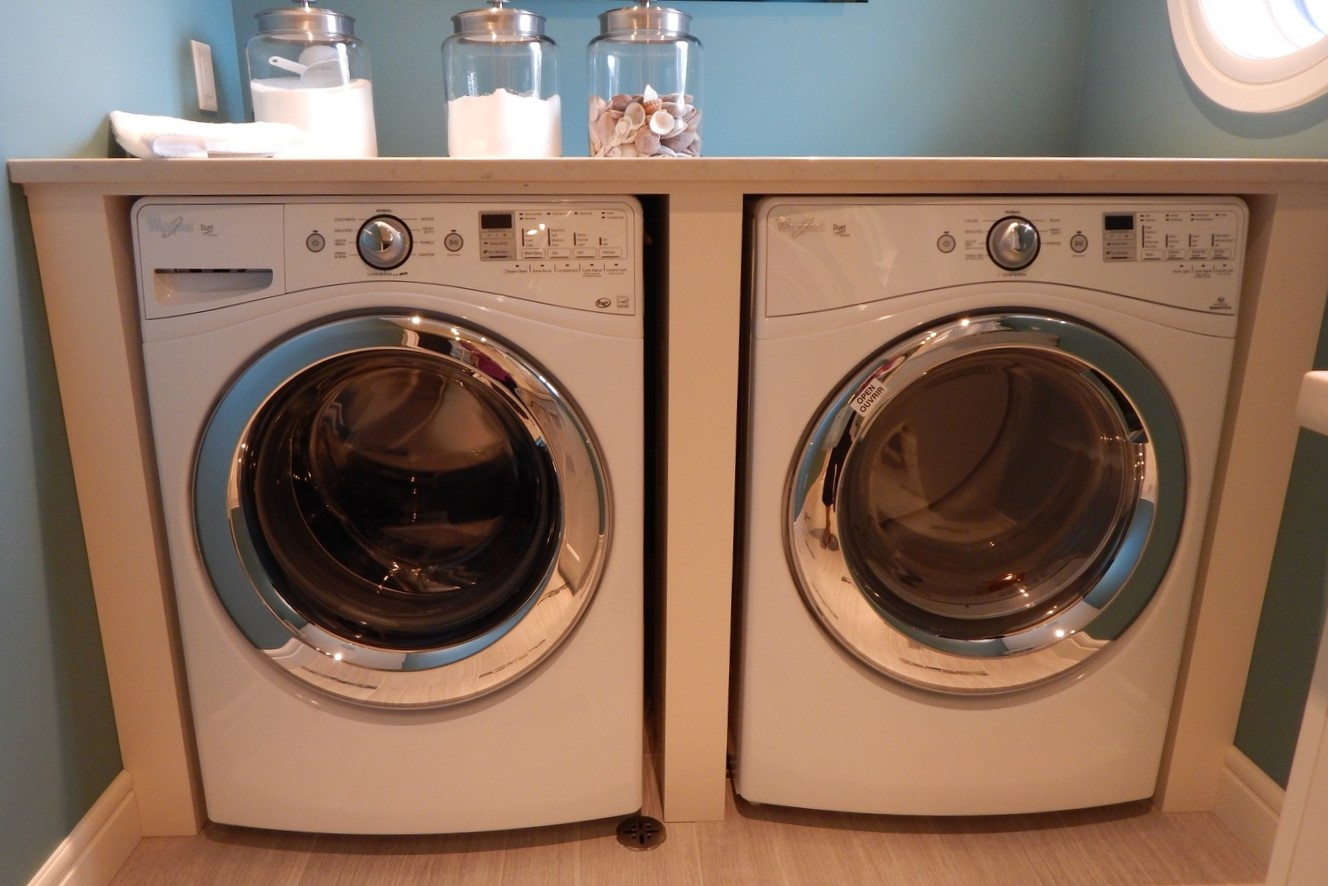
\includegraphics[width=0.5\textwidth]{fig/lec01/Home_appliance.jpg}
			\caption{Home appliances (source: \href{https://pxhere.com/de/photo/863012}{pxhere}, \href{https://creativecommons.org/publicdomain/zero/1.0/}{CC0~1.0})}
		\end{subfigure}
		\pause
		\hfill
		\begin{subfigure}[b]{0.49\textwidth}
			\centering
			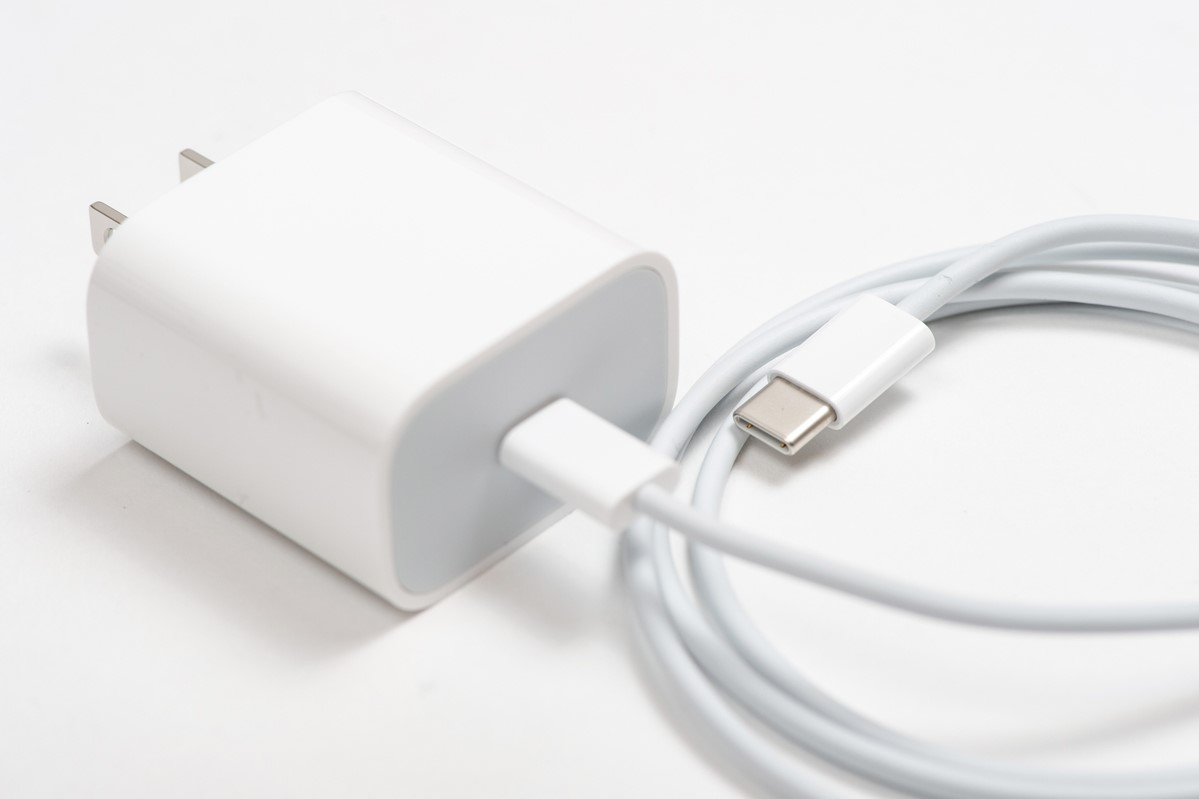
\includegraphics[width=0.5\textwidth]{fig/lec01/Smartphone_charger.jpg}
			\caption{Smartphone charger (source: \href{https://www.rawpixel.com/image/5923136/photo-image-phone-public-domain-white}{rawpixel}, \href{https://creativecommons.org/publicdomain/zero/1.0/}{CC0~1.0})}
		\end{subfigure}
		\pause
		\\
		\begin{subfigure}[b]{0.49\textwidth}
			\centering
			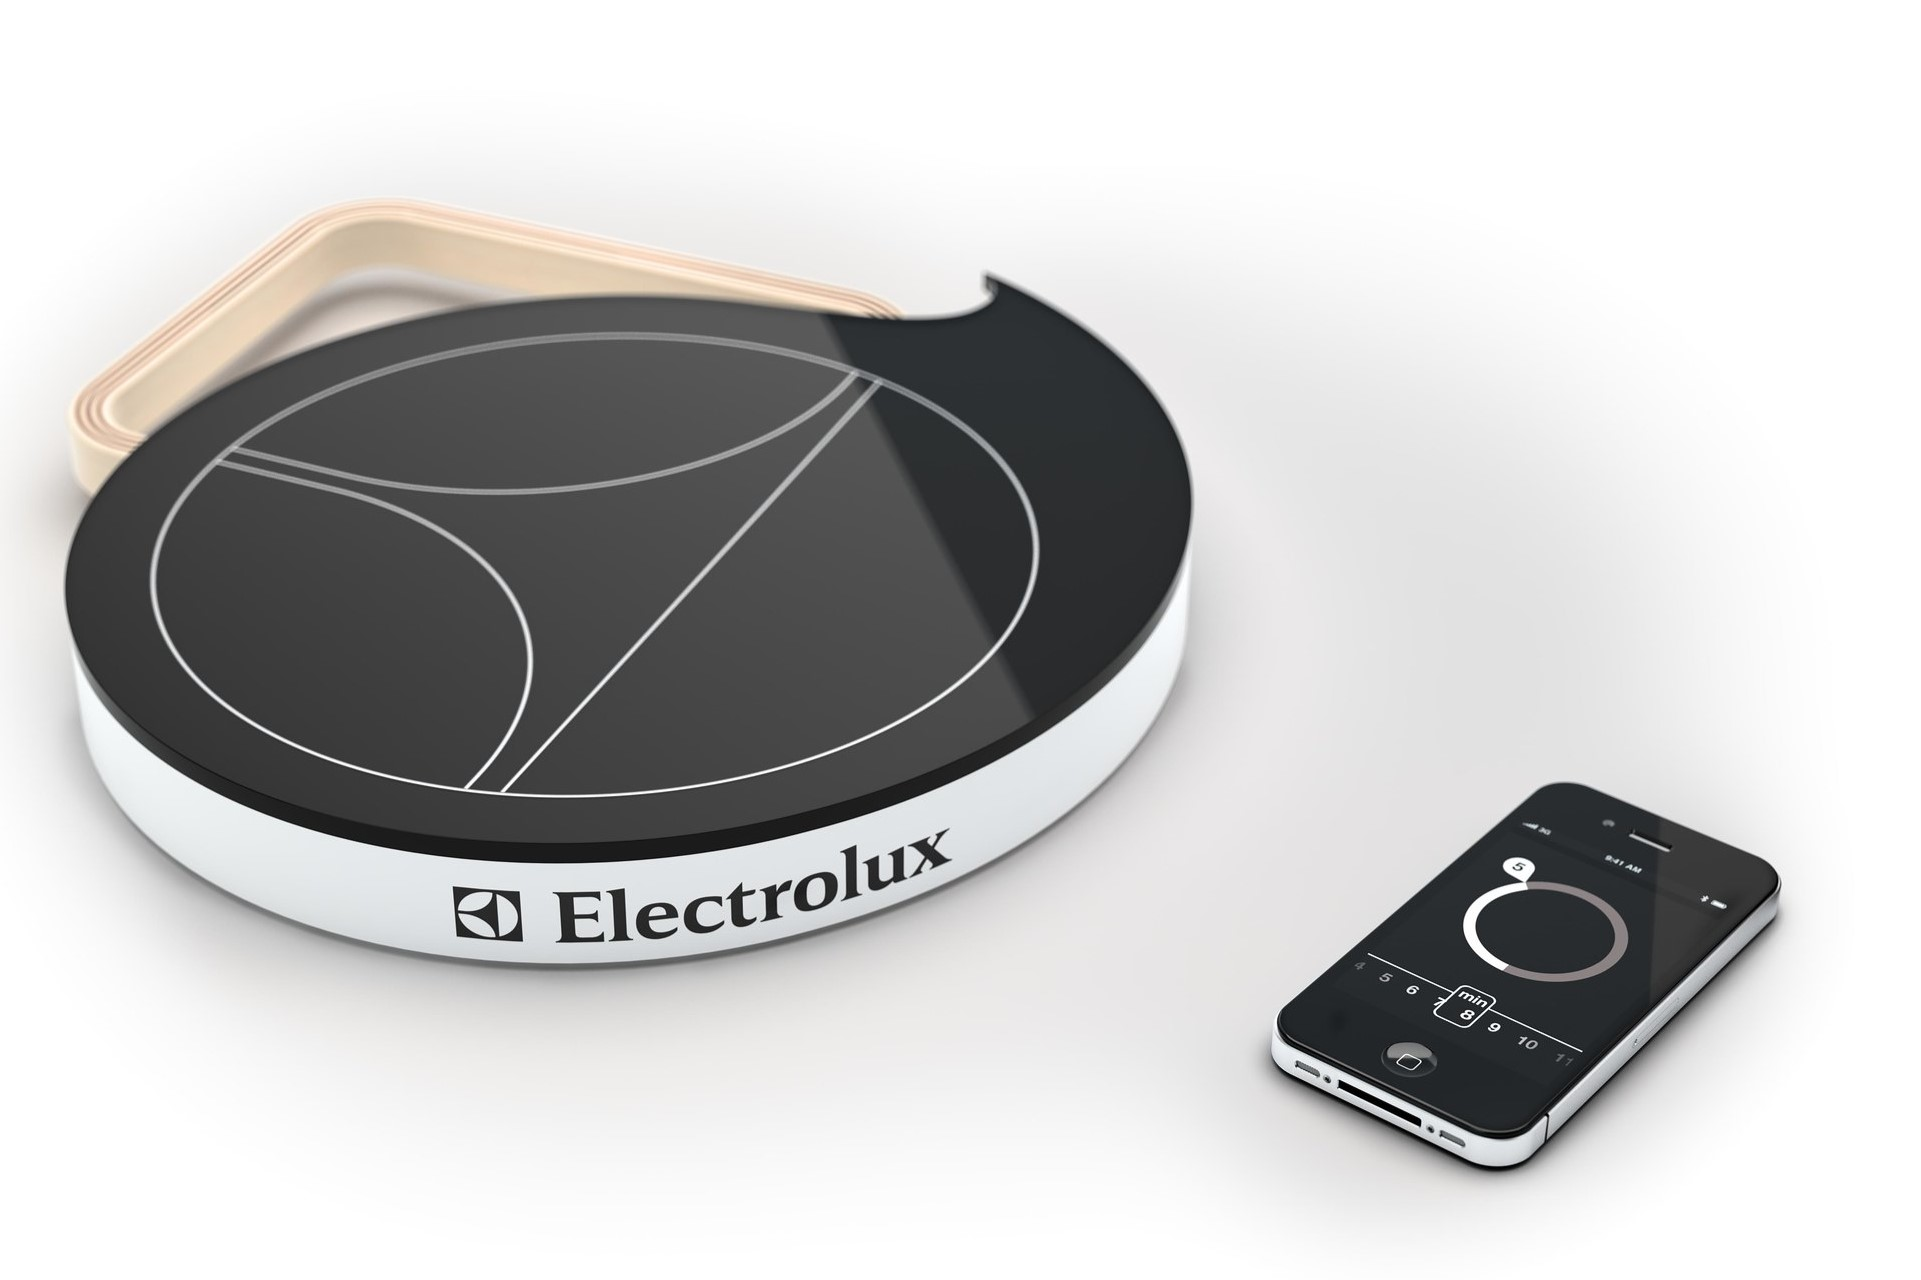
\includegraphics[width=0.5\textwidth]{fig/lec01/Induction_plate.jpg}
			\caption{Induction plate (source: \href{https://www.flickr.com/photos/electrolux-design-lab/6035618944}{flickr}, Electrolux, \href{https://creativecommons.org/licenses/by-nc/2.0/}{CC~BY-SA-NC~2.0})}
		\end{subfigure}
		\pause
		\hfill
		\begin{subfigure}[b]{0.49\textwidth}
			\centering
			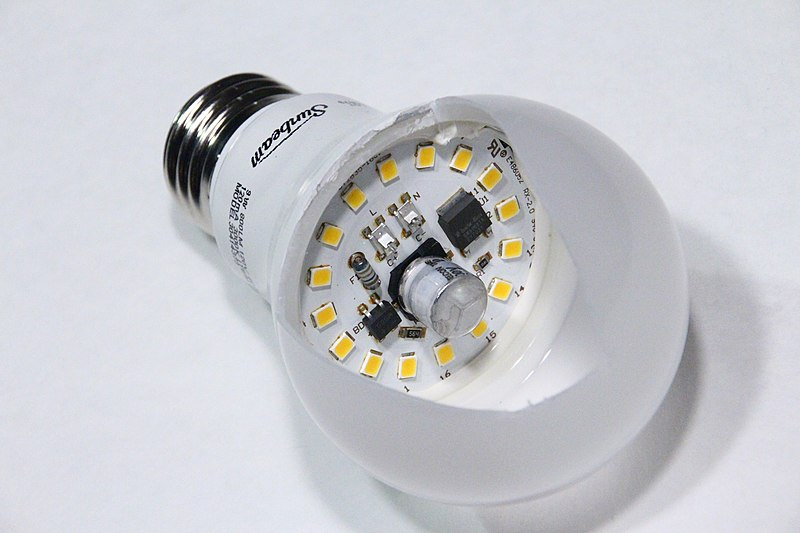
\includegraphics[width=0.5\textwidth]{fig/lec01/LED_light_bulb.jpg}
			\caption{LED rectifier (source: \href{https://commons.wikimedia.org/wiki/File:LED-E27-Light-Bulb-1134.jpg}{Wikimedia Commons}, D.~Tribble, \href{https://creativecommons.org/licenses/by-sa/4.0/deed.en}{CC~BY-SA~4.0})}
		\end{subfigure}
	\end{figure}
\end{frame}

%%%%%%%%%%%%%%%%%%%%%%%%%%%%%%%%%%%%%%%%%%%%%%%%%%%%%%%%%%%%%
%% Power electronic application examples: industrial %%
%%%%%%%%%%%%%%%%%%%%%%%%%%%%%%%%%%%%%%%%%%%%%%%%%%%%%%%%%%%%%
\begin{frame}[c]
	\frametitle{Power electronic application examples: industrial}
	\begin{figure}
		\centering
		\begin{subfigure}[b]{0.49\textwidth}
			\centering
			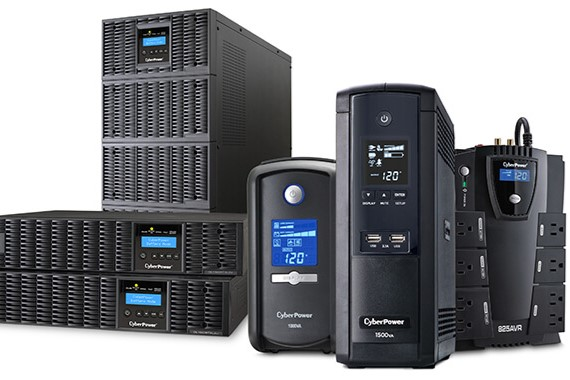
\includegraphics[width=0.5\textwidth]{fig/lec01/UPS.jpg}
			\caption{Uninterruptible power supply (source: \href{https://commons.wikimedia.org/wiki/File:CyberPower_UPS_Systems.jpg}{Wikimedia Commons}, Stevebwallace, \href{https://creativecommons.org/licenses/by-sa/4.0/deed.en}{CC~BY-SA~4.0})}
		\end{subfigure}
		\pause
		\hfill
		\begin{subfigure}[b]{0.49\textwidth}
			\centering
			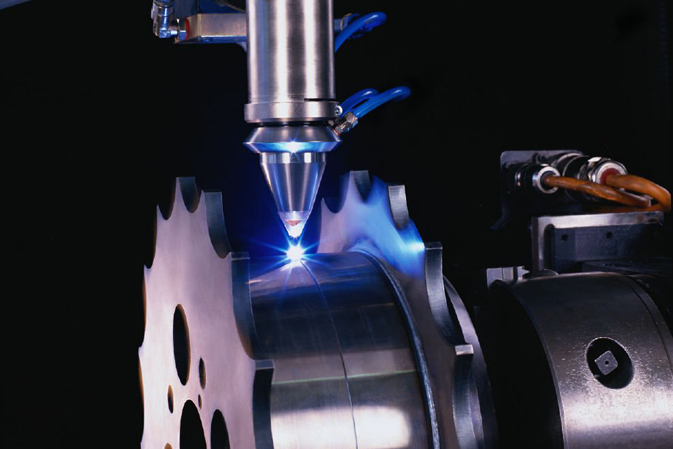
\includegraphics[width=0.5\textwidth]{fig/lec01/Welding.jpg}
			\caption{Welding power supply (source: \href{https://commons.wikimedia.org/wiki/File:Trumpf_laserschweissen.jpg}{Wikimedia Commons}, Trumpf GmbH, \href{https://creativecommons.org/licenses/by-sa/3.0/deed.en}{CC~BY-SA~3.0})}
		\end{subfigure}
		\pause
		\\
		\begin{subfigure}[b]{0.49\textwidth}
			\centering
			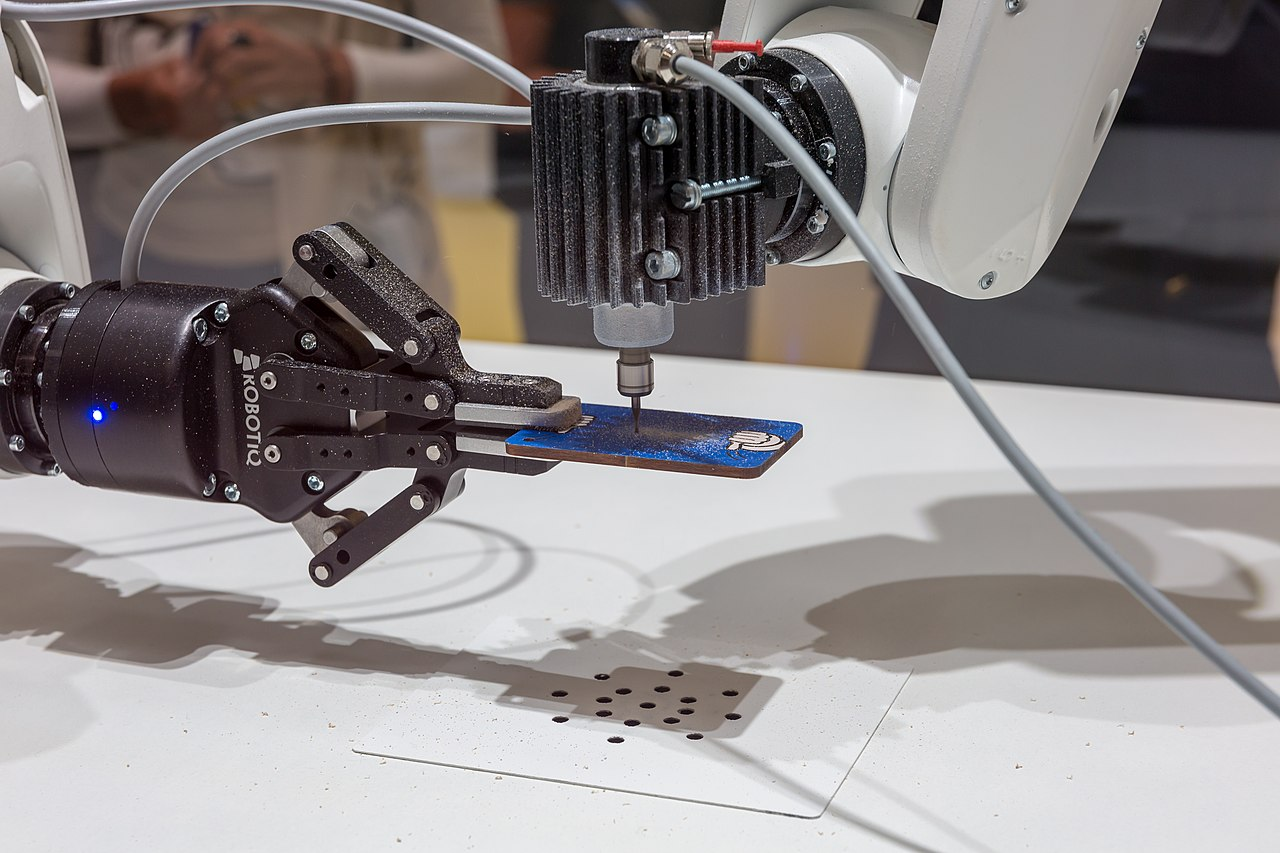
\includegraphics[width=0.5\textwidth]{fig/lec01/Robot.jpg}
			\caption{Industrial drives / automation (source: \href{https://de.m.wikipedia.org/wiki/Datei:Paris_Motor_Show_2018,_Paris_\%281Y7A1752\%29.jpg}{Wikimedia Commons}, M.~Blume, \href{https://creativecommons.org/licenses/by-sa/4.0/deed.de}{CC~BY-SA~4.0})}
		\end{subfigure}
		\pause
		\hfill
		\begin{subfigure}[b]{0.49\textwidth}
			\centering
			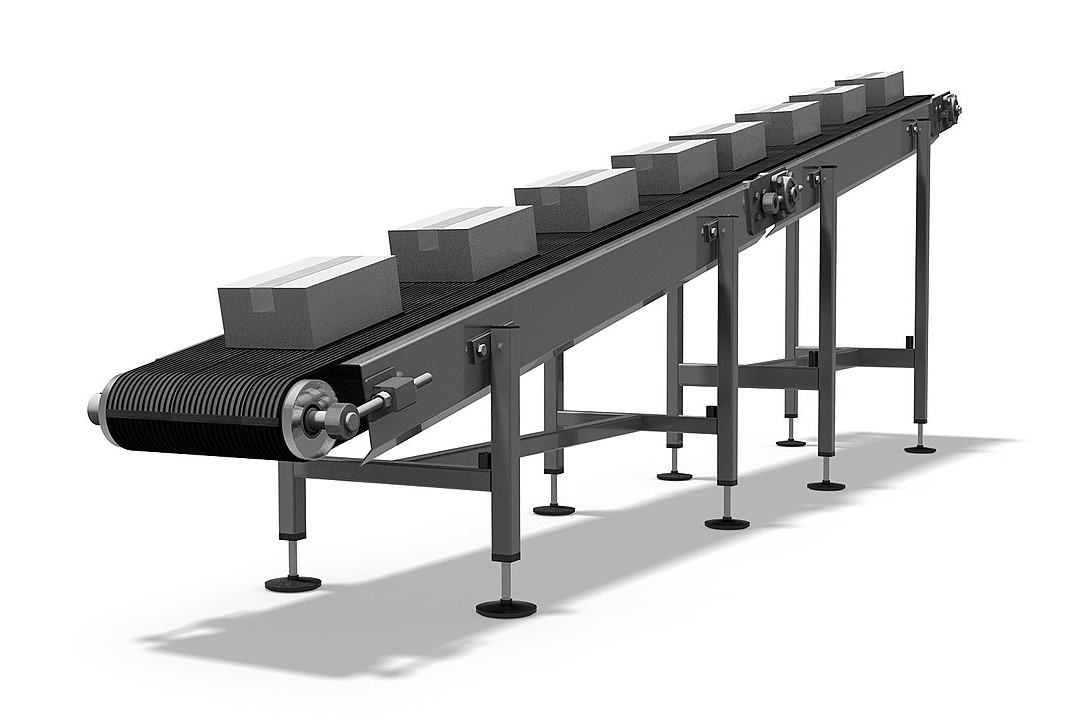
\includegraphics[width=0.5\textwidth]{fig/lec01/Conveyor.jpg}
			\caption{Conveyor belt drive (source: \href{https://commons.wikimedia.org/wiki/File:Inclined-belt_conveyor.jpgg}{Wikimedia Commons},  	K.~Hannessen, \href{https://creativecommons.org/licenses/by-sa/4.0/deed.en}{CC~BY-SA~4.0})}
		\end{subfigure}
	\end{figure}
\end{frame}

%%%%%%%%%%%%%%%%%%%%%%%%%%%%%%%%%%%%%%%%%%%%%%%%%%%%%%%%%%%%%
%% Power electronic application examples: energy system %%
%%%%%%%%%%%%%%%%%%%%%%%%%%%%%%%%%%%%%%%%%%%%%%%%%%%%%%%%%%%%%
\begin{frame}[c]
	\frametitle{Power electronic application examples: energy system}
	\begin{figure}
		\centering
		\begin{subfigure}[b]{0.49\textwidth}
			\centering
			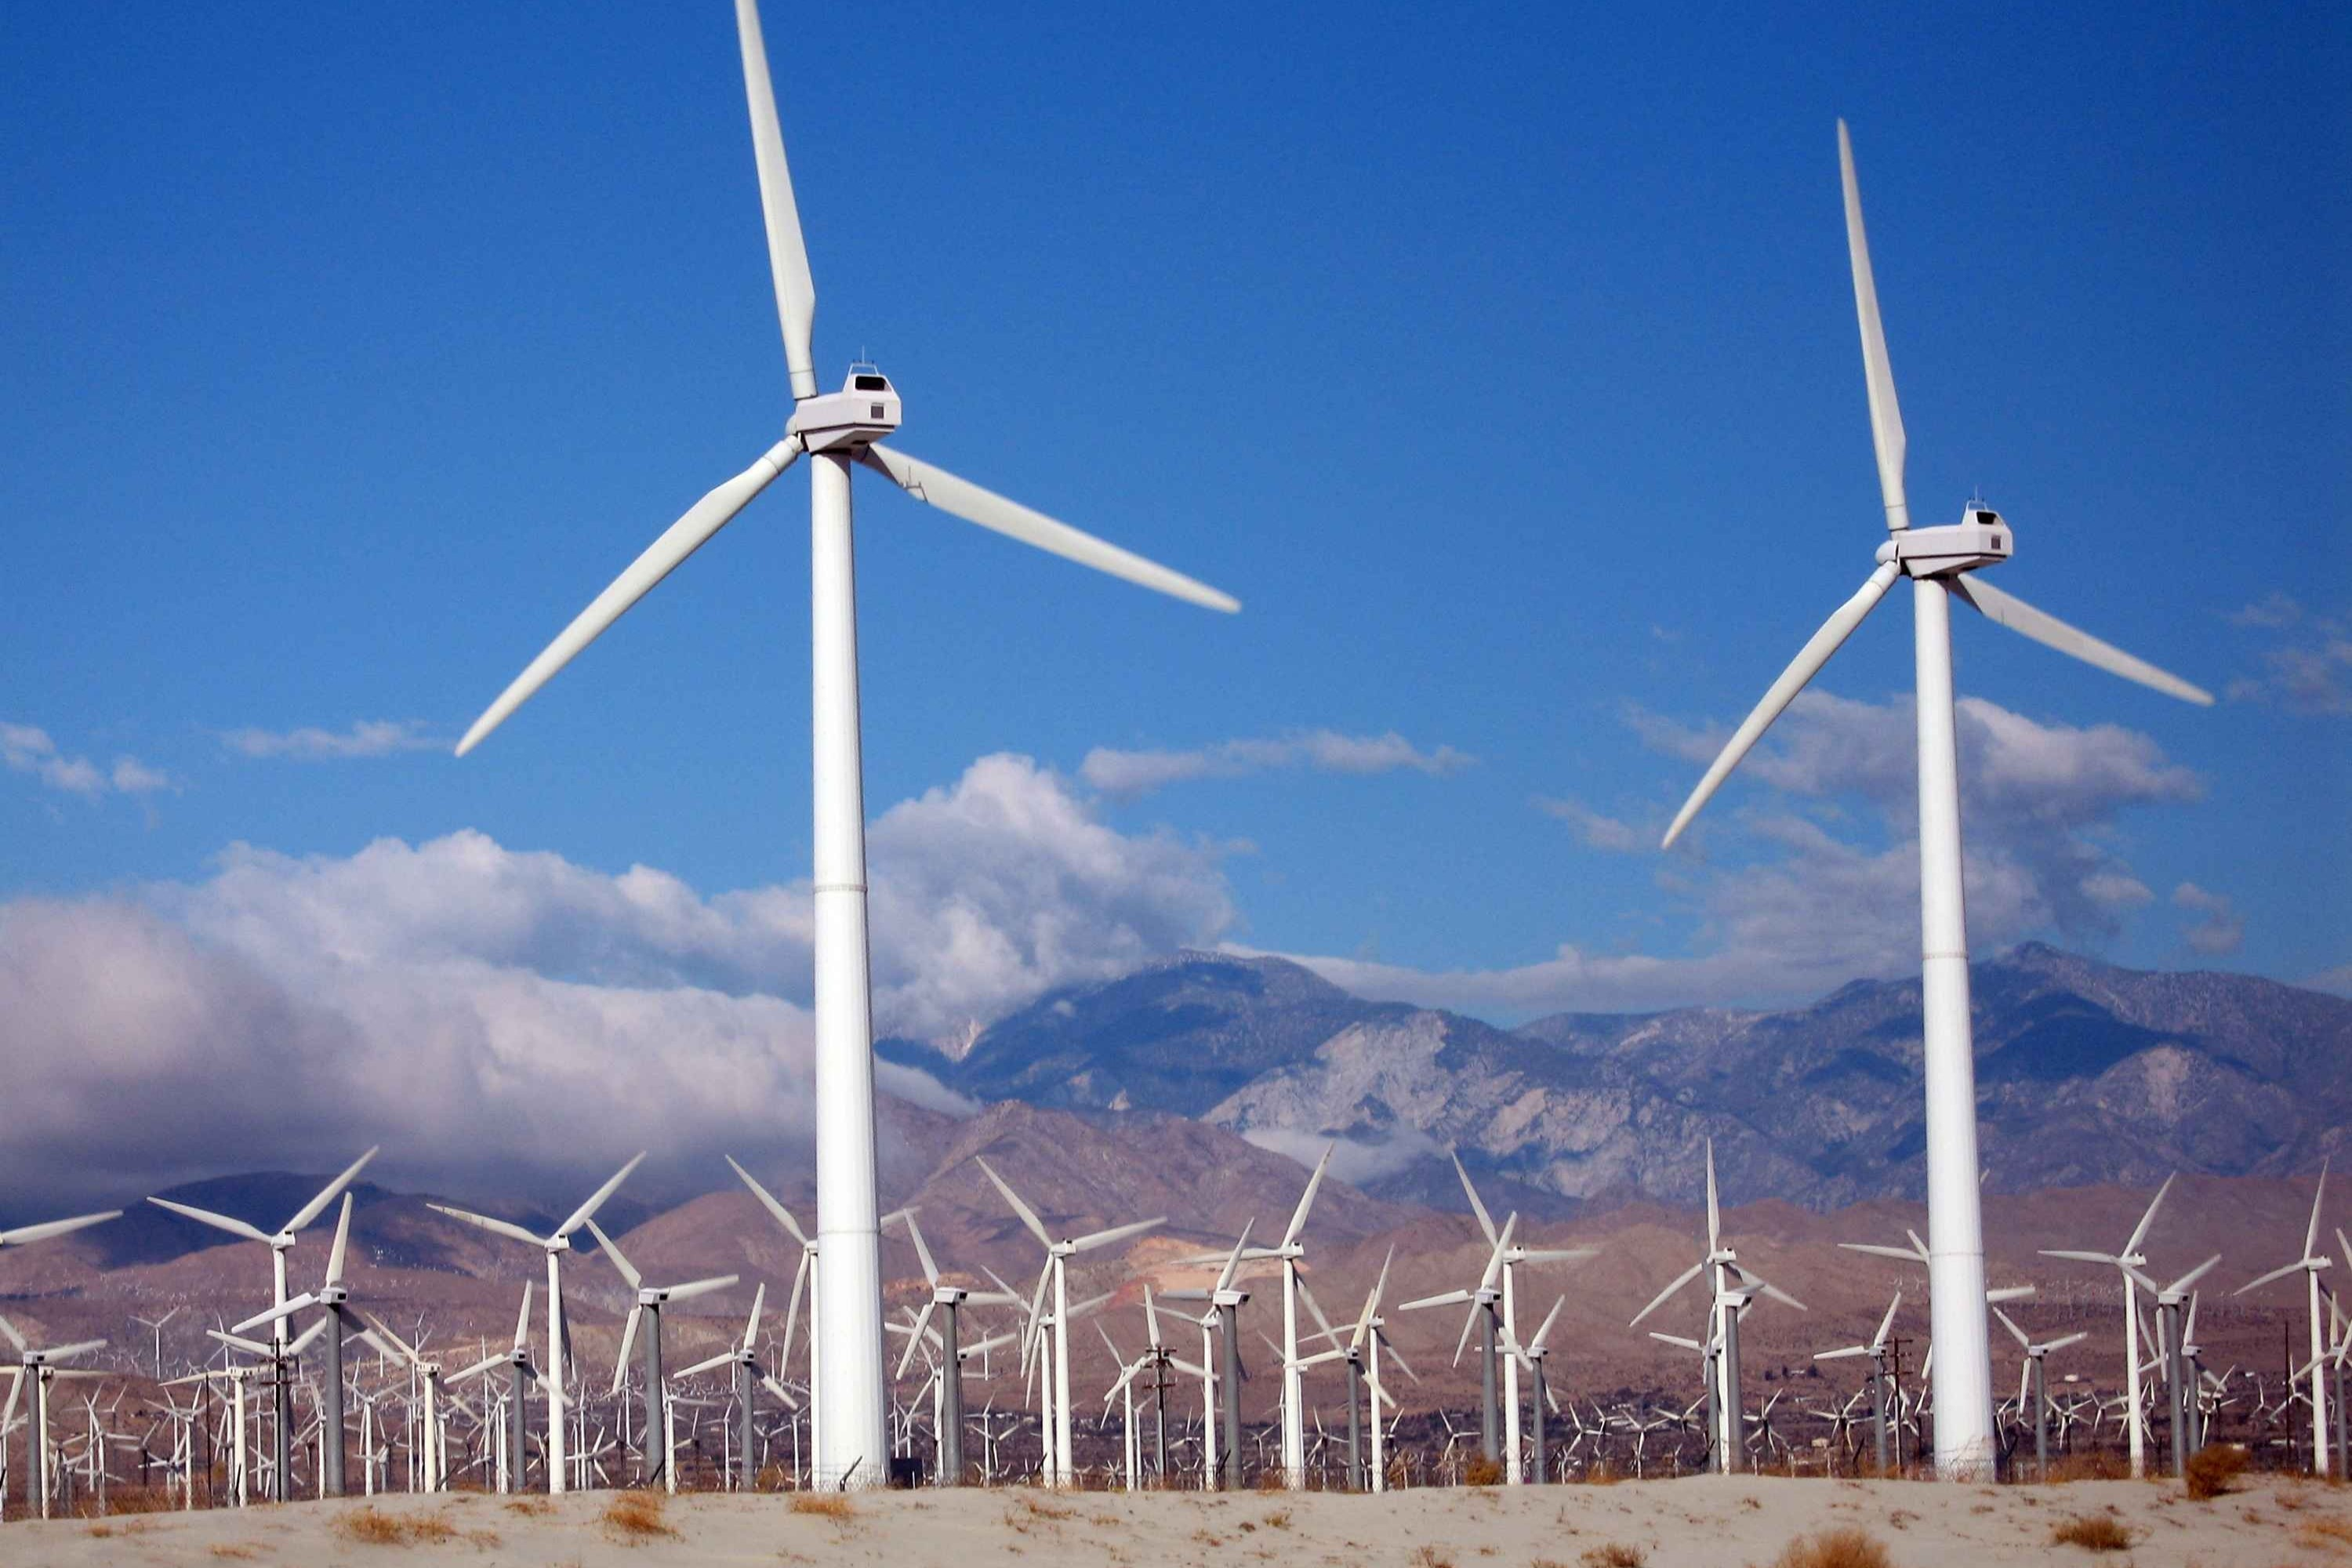
\includegraphics[width=0.5\textwidth]{fig/lec01/sky-farm-windmill.jpg}
			\caption{Wind power plants (source: \href{https://pxhere.com/en/photo/954757}{pxhere}, \href{https://creativecommons.org/publicdomain/zero/1.0/}{CC0~1.0})}
		\end{subfigure}
		\pause
		\hfill
		\begin{subfigure}[b]{0.49\textwidth}
			\centering
			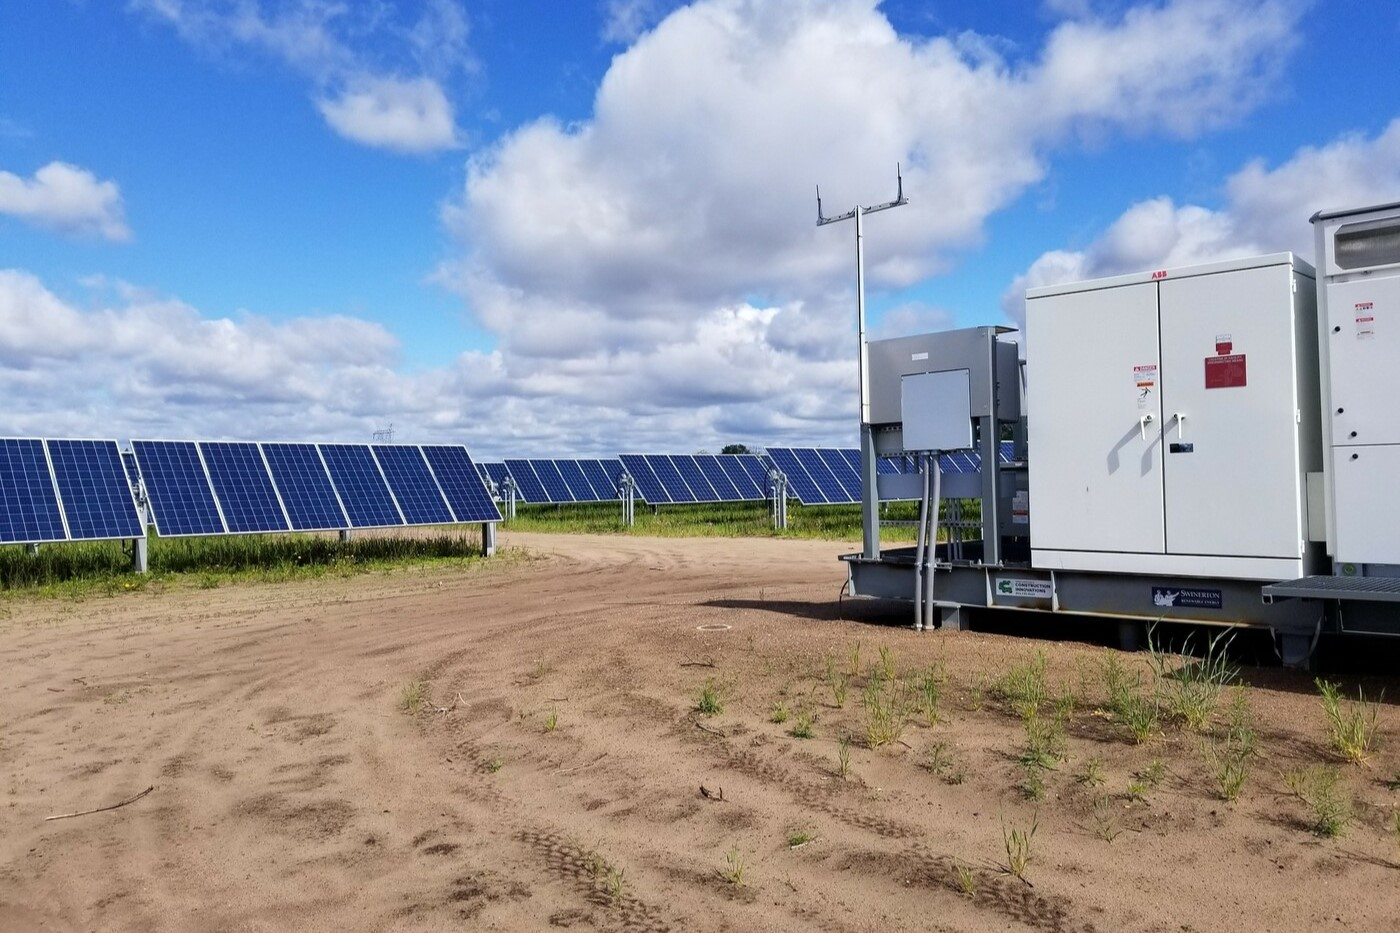
\includegraphics[width=0.5\textwidth]{fig/lec01/PV_field.jpg}
			\caption{PV power plants (source: \href{https://pxhere.com/en/photo/1685464}{pxhere}, \href{https://creativecommons.org/publicdomain/zero/1.0/}{CC0~1.0})}
		\end{subfigure}
		\pause
		\\
		\begin{subfigure}[b]{0.49\textwidth}
			\centering
			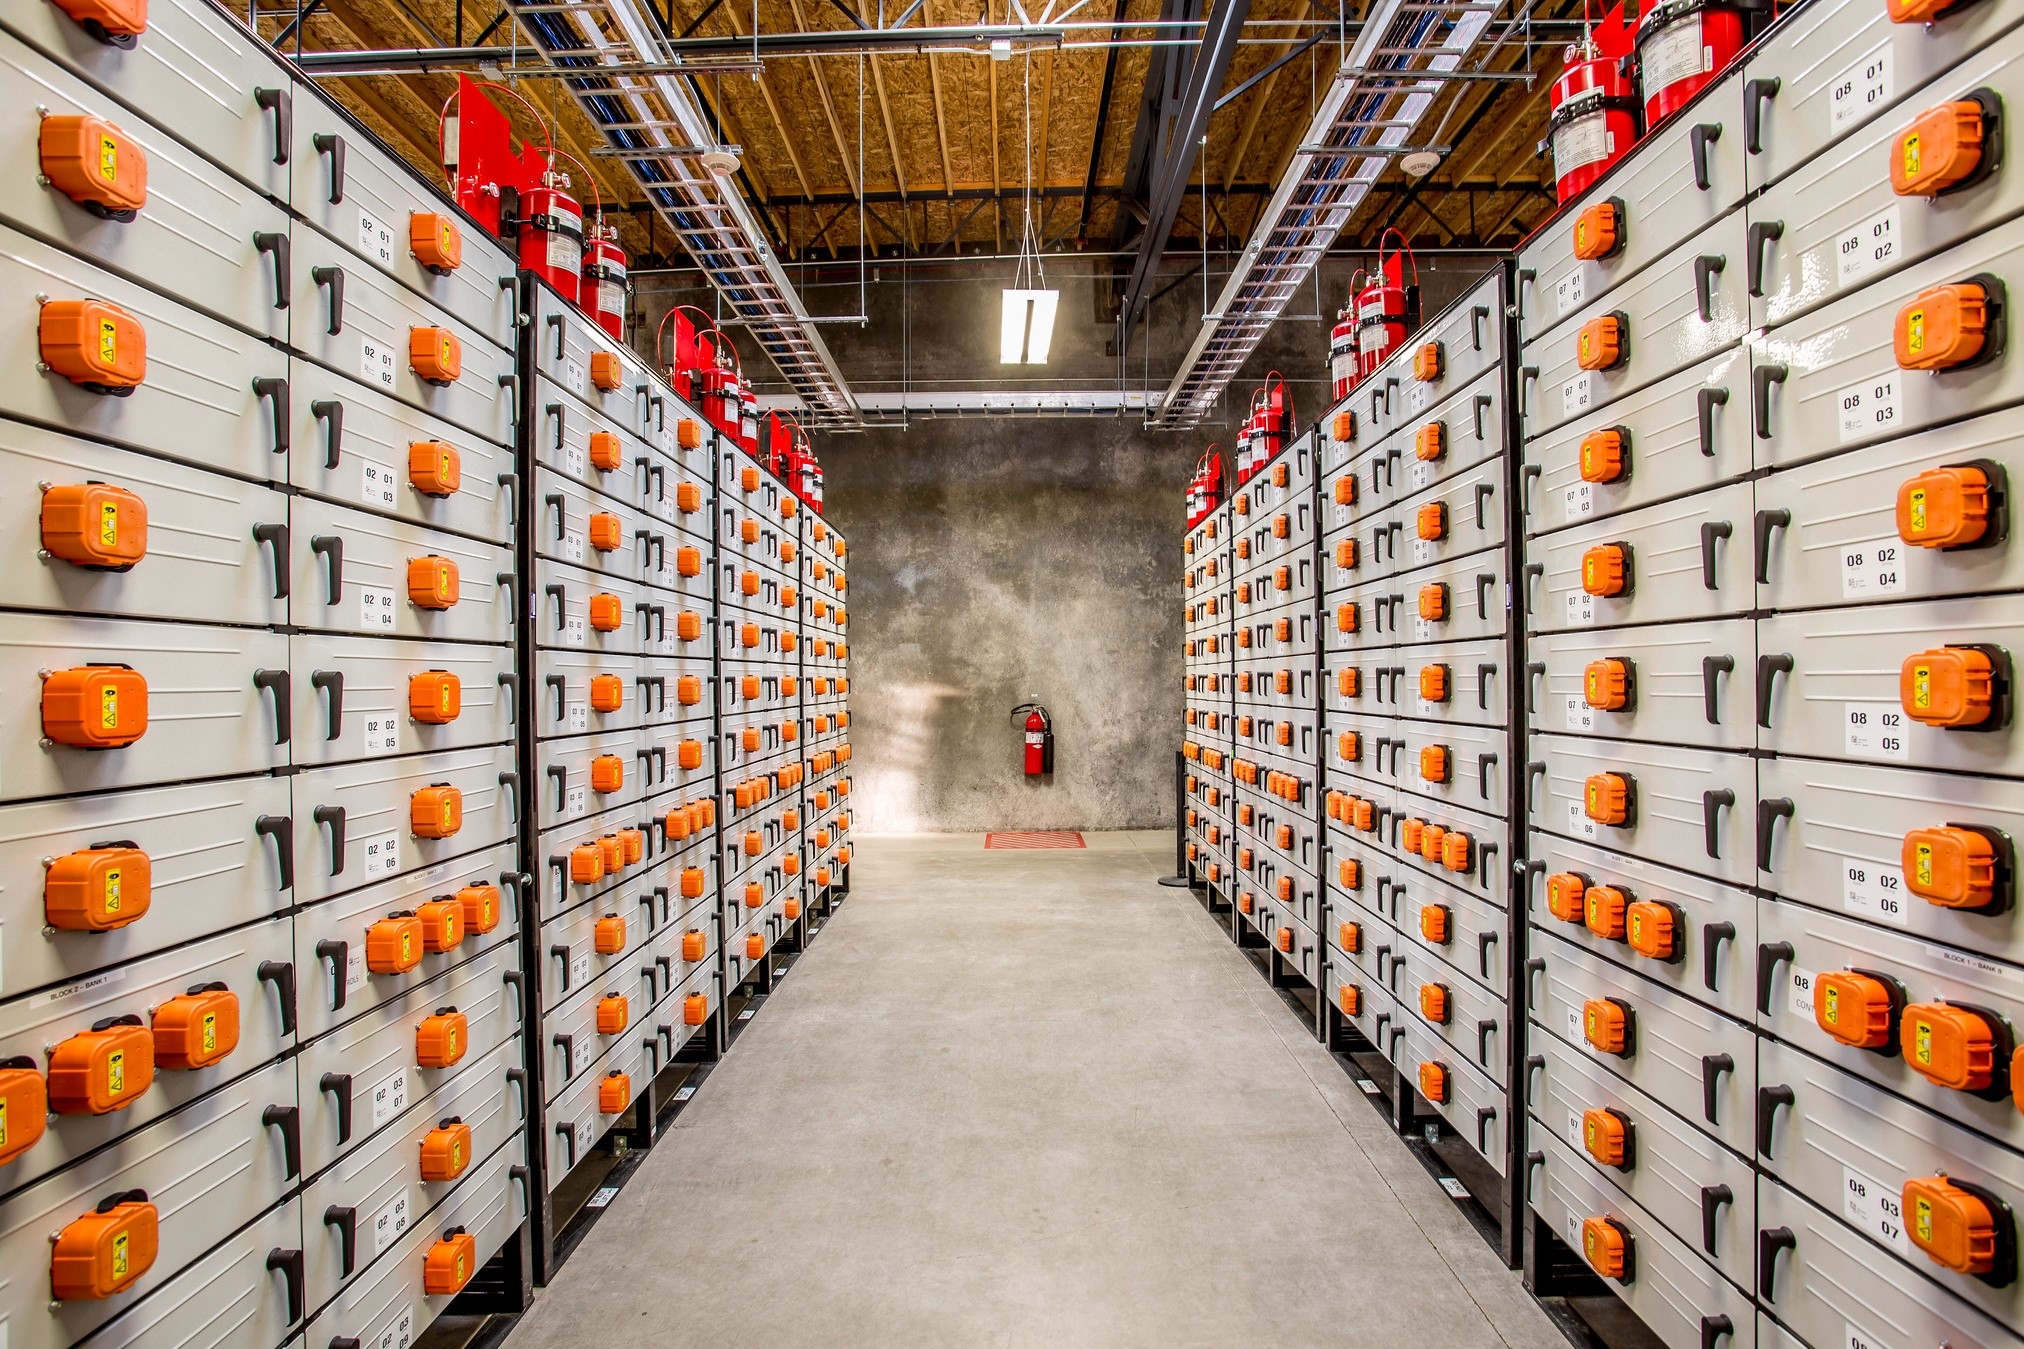
\includegraphics[width=0.5\textwidth]{fig/lec01/Battery_storage.jpg}
			\caption{Battery storage systems (source: \href{https://www.flickr.com/photos/portlandgeneralelectric/8905201835}{flickr}, 
			Portland General Electric, \href{https://creativecommons.org/licenses/by-nd/2.0/}{CC~BY-ND~2.0})}
		\end{subfigure}
		\pause
		\hfill
		\begin{subfigure}[b]{0.49\textwidth}
			\centering
			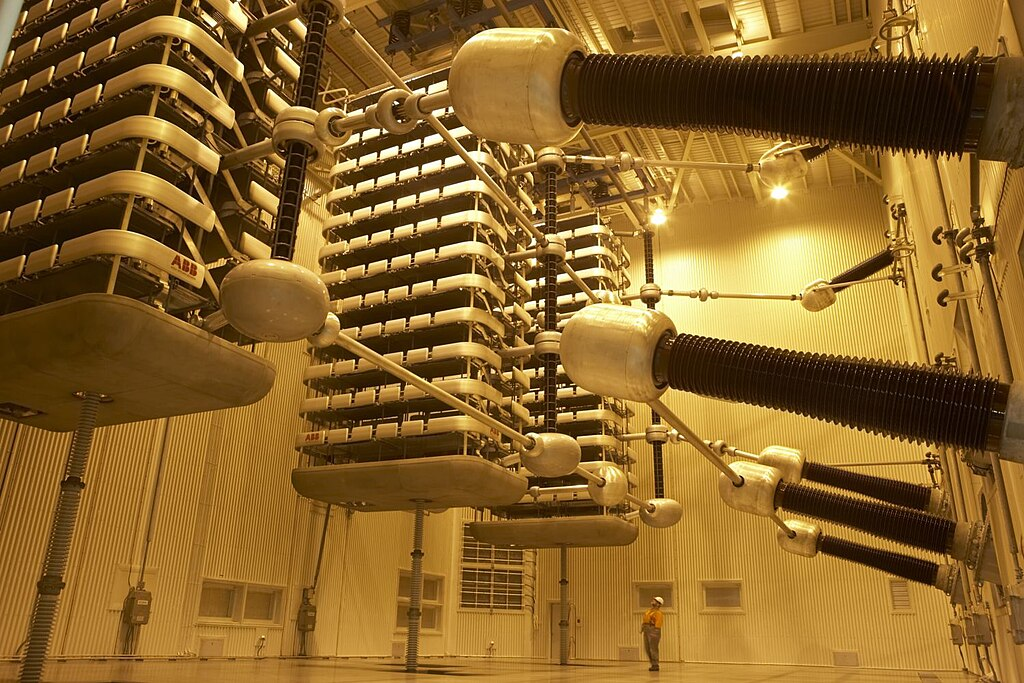
\includegraphics[width=0.5\textwidth]{fig/lec01/HVDC.jpg}
			\caption{High voltage DC transmission (source: \href{https://commons.wikimedia.org/wiki/File:Pole_2_Thyristor_Valve.jpg}{Wikimedia Commons},  	 	Marshelec, \href{https://creativecommons.org/licenses/by-sa/3.0/deed.en}{CC~BY-SA~3.0})}
		\end{subfigure}
	\end{figure}
\end{frame}

%%%%%%%%%%%%%%%%%%%%%%%%%%%%%%%%%%%%%%%%%%%%%%%%%%%%%%%%%%%%%
%% Power electronic application examples: transportation %%
%%%%%%%%%%%%%%%%%%%%%%%%%%%%%%%%%%%%%%%%%%%%%%%%%%%%%%%%%%%%%
\begin{frame}[c]
	\frametitle{Power electronic application examples: transportation}
	\begin{figure}
		\centering
		\begin{subfigure}[b]{0.49\textwidth}
			\centering
			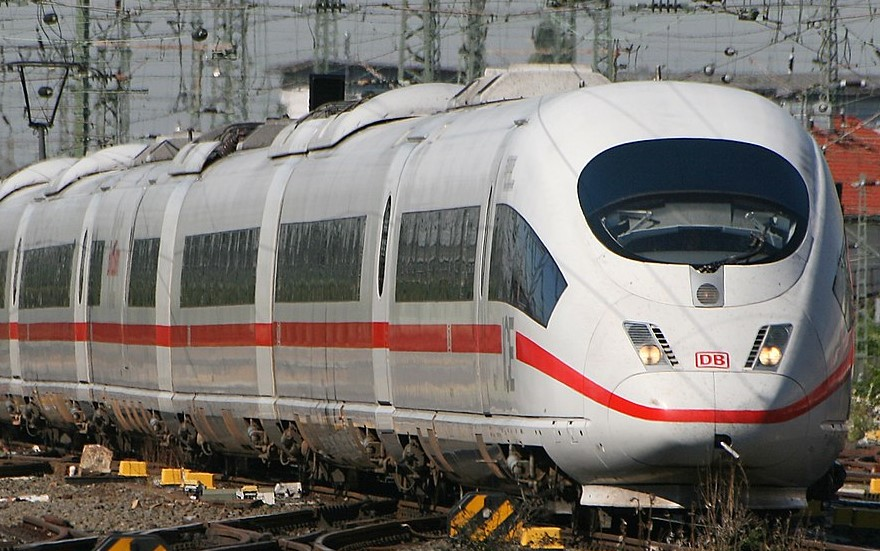
\includegraphics[width=0.5\textwidth]{fig/lec01/ICE.jpg}
			\caption{Train drive (source: \href{hhttps://commons.wikimedia.org/wiki/File:DB_AG_406_001-8.jpg}{Wikimedia Commons}, T.~Wolf, \href{https://creativecommons.org/publicdomain/zero/1.0/}{CC0~1.0})}
		\end{subfigure}
		\pause
		\hfill
		\begin{subfigure}[b]{0.49\textwidth}
			\centering
			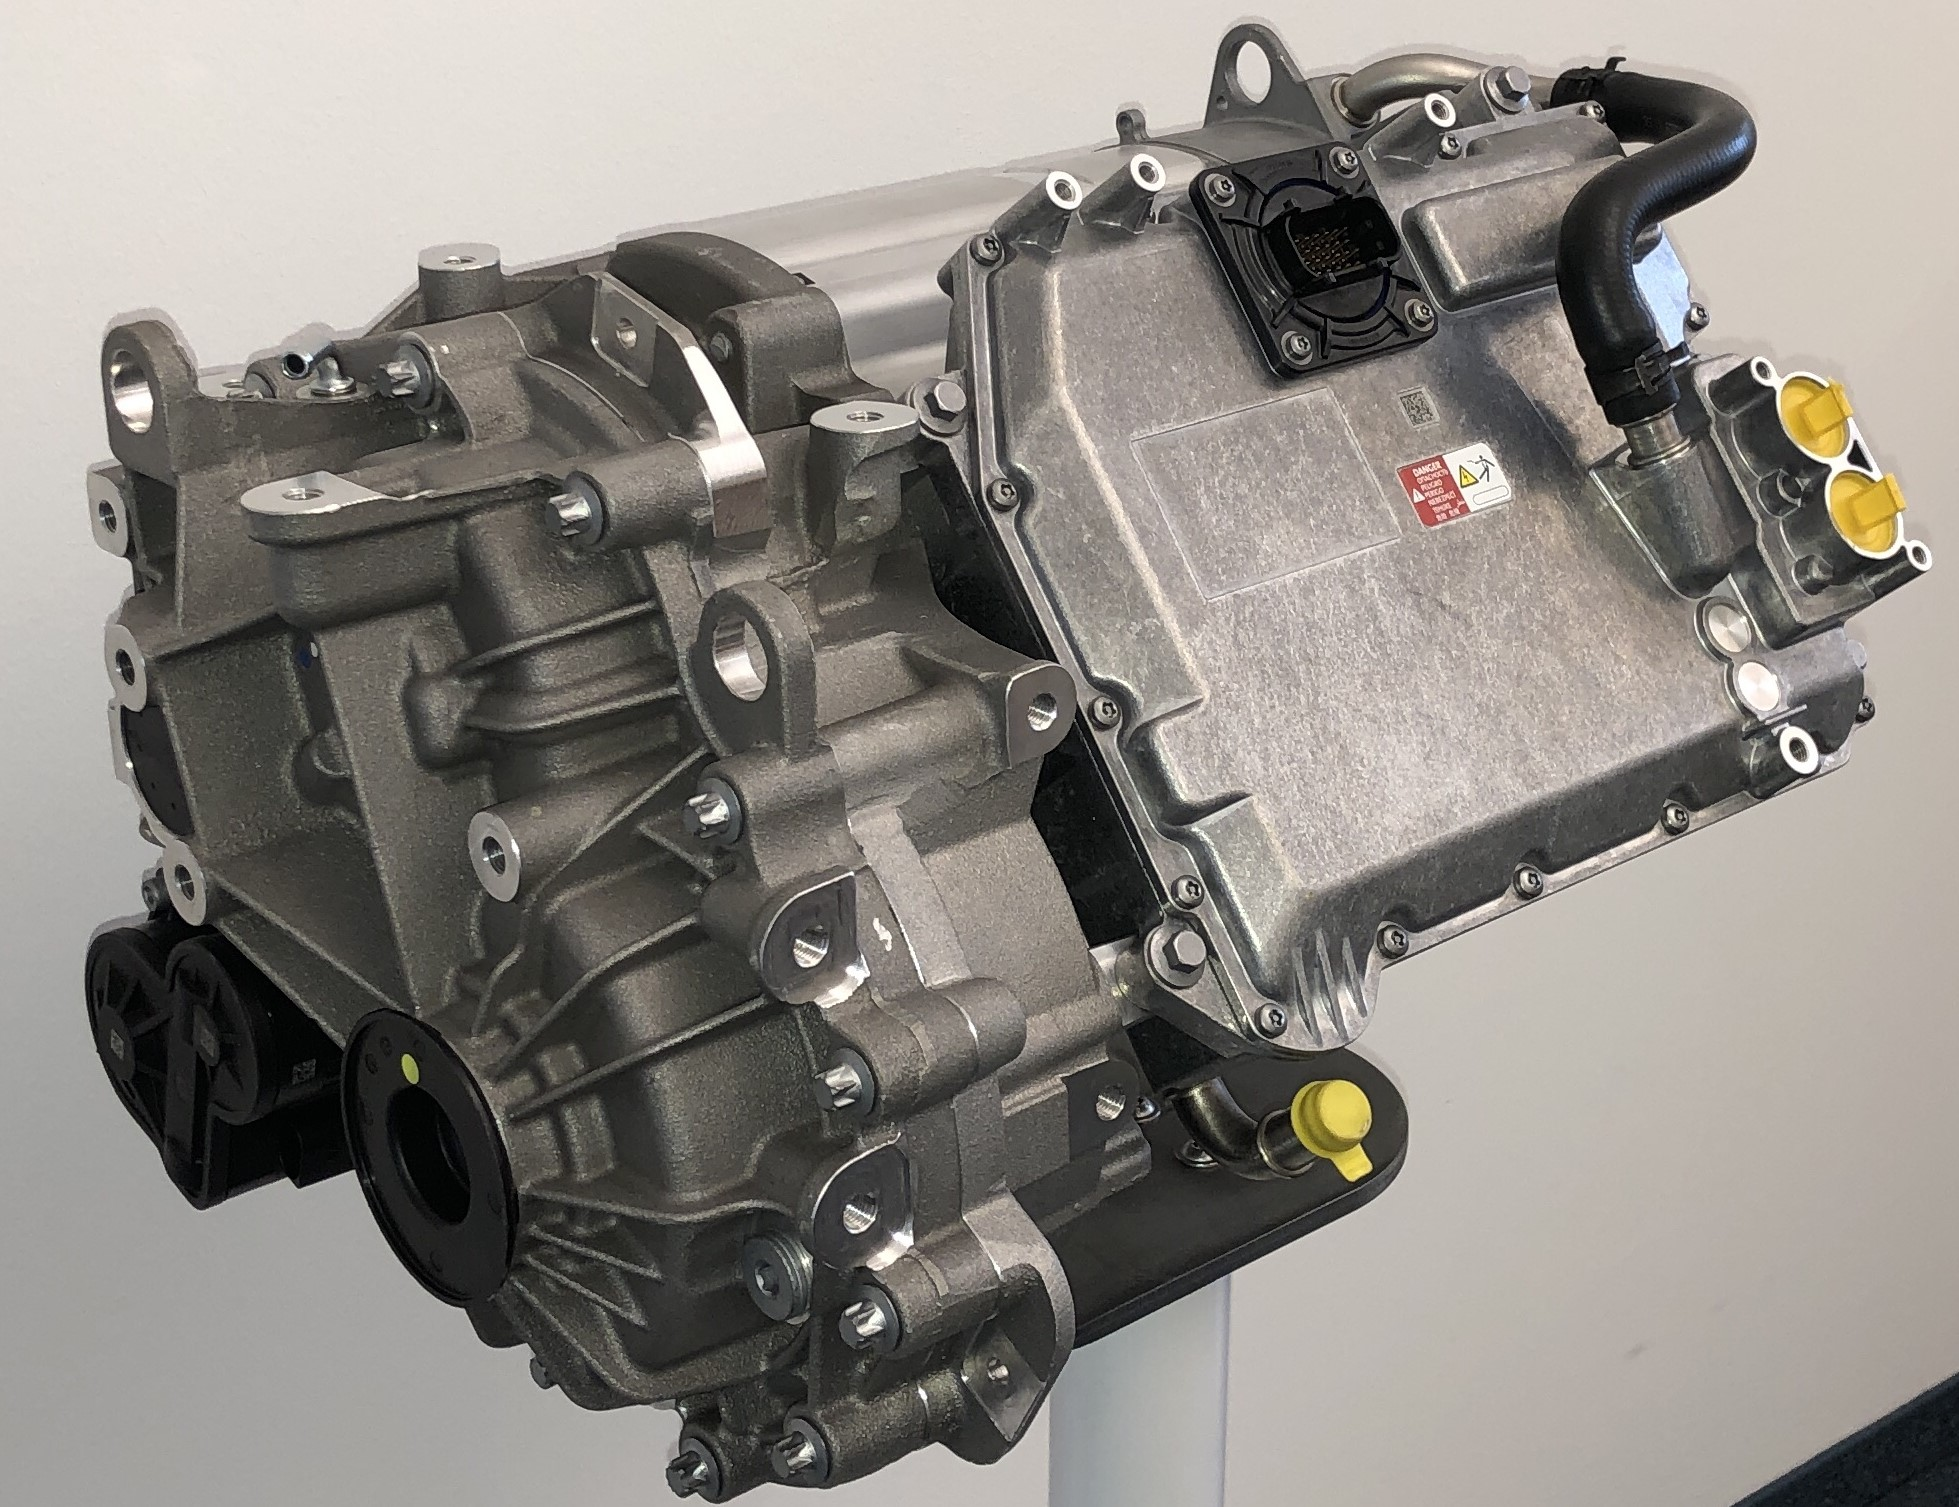
\includegraphics[width=0.5\textwidth]{fig/lec01/Drive.jpg}
			\caption{Electric vehicle drive (source: \href{https://commons.wikimedia.org/wiki/File:Vitesco_Technologies_EMR3.jpg}{Wikimedia Commons}, Caprolactam123, \href{https://creativecommons.org/licenses/by-sa/4.0/deed.en}{CC~BY-SA~4.0})}
		\end{subfigure}
		\pause
		\\
		\begin{subfigure}[b]{0.49\textwidth}
			\centering
			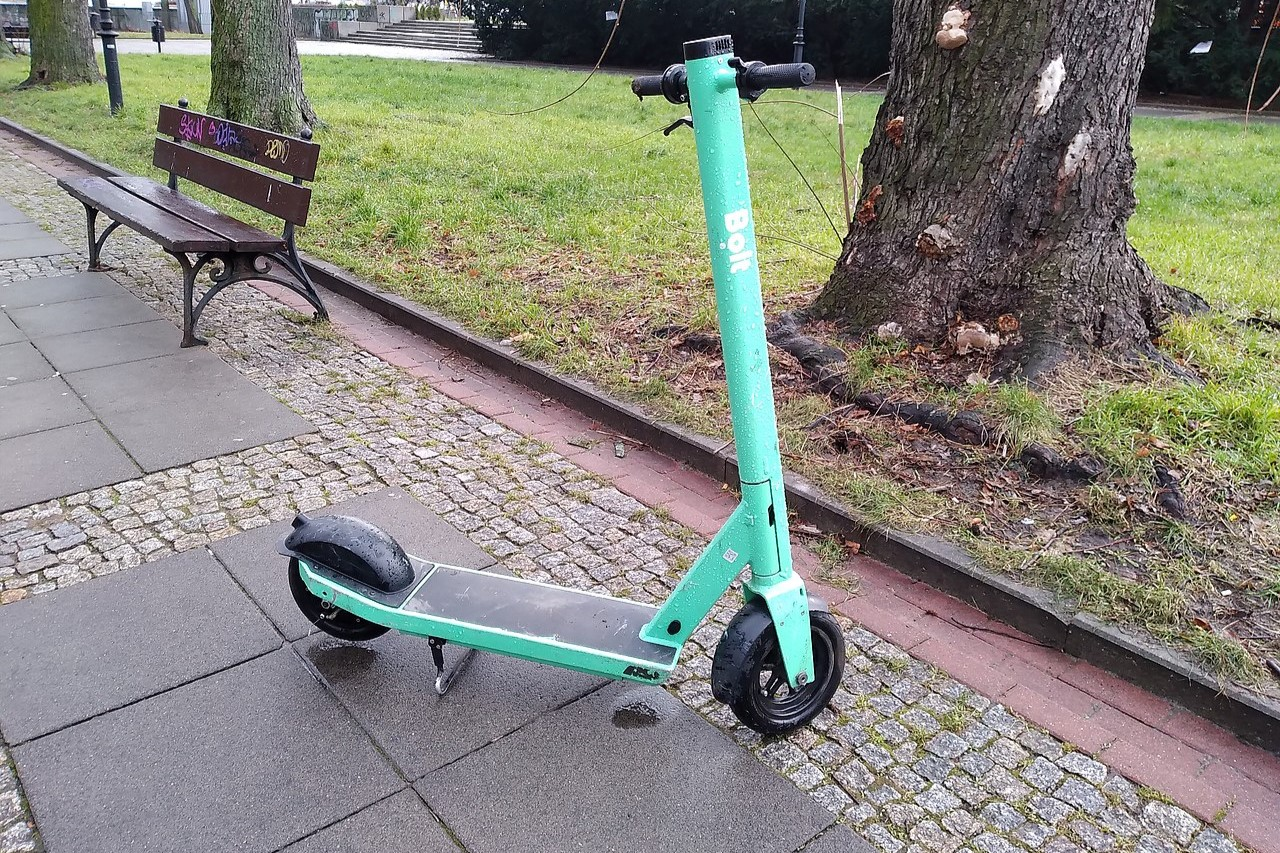
\includegraphics[width=0.5\textwidth]{fig/lec01/Scooter.jpg}
			\caption{Electric scooter (source: \href{https://commons.wikimedia.org/wiki/File:Bolt_Electric_Scooter_\%28Warsaw\%29_in_2020.03.jpg}{Wikimedia Commons}, Raju, \href{https://creativecommons.org/licenses/by-sa/4.0/deed.en}{CC~BY-SA~4.0})}
		\end{subfigure}
		\pause
		\hfill
		\begin{subfigure}[b]{0.49\textwidth}
			\centering
			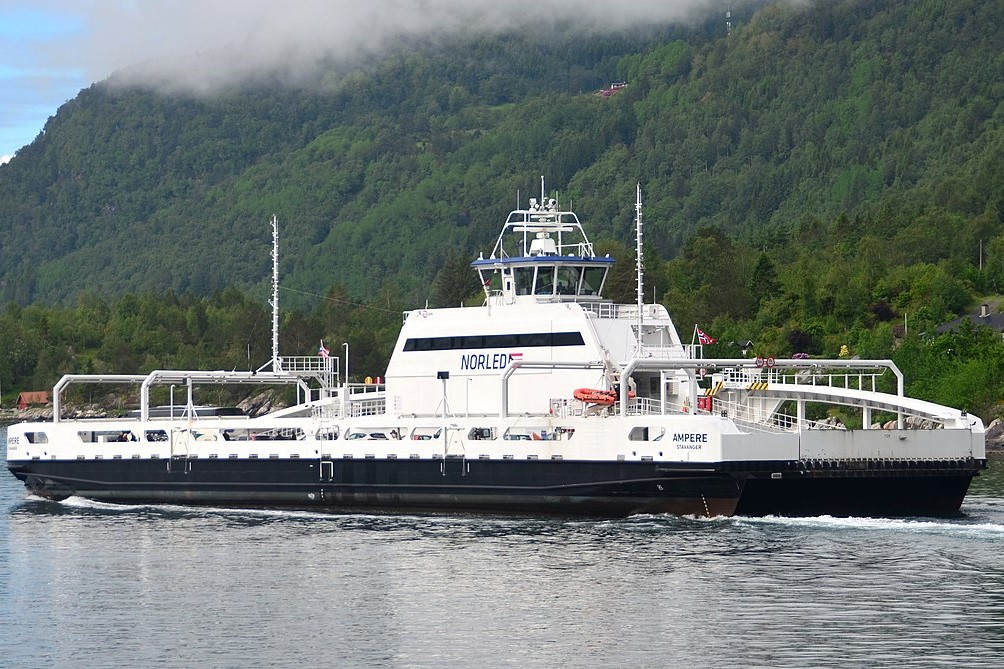
\includegraphics[width=0.5\textwidth]{fig/lec01/Electric_ship.jpg}
			\caption{Electic ship (source: \href{https://commons.wikimedia.org/wiki/File:Ferry_Ampere_Sognefjord.jpg}{Wikimedia Commons},  	 	Wikimalte, \href{https://creativecommons.org/licenses/by-sa/4.0/deed.en}{CC~BY-SA~4.0})}
		\end{subfigure}
	\end{figure}
\end{frame}

%%%%%%%%%%%%%%%%%%%%%%%%%%%%%%%%%%%%%%%%%%%%%%%%%%%%%%%%%%%%%
%% A broad range of nominal power ratings %%
%%%%%%%%%%%%%%%%%%%%%%%%%%%%%%%%%%%%%%%%%%%%%%%%%%%%%%%%%%%%%
\begin{frame}[c]
	\frametitle{A broad range of nominal power ratings}
	\vspace{0.3cm}
	\begin{figure}
		\centering
		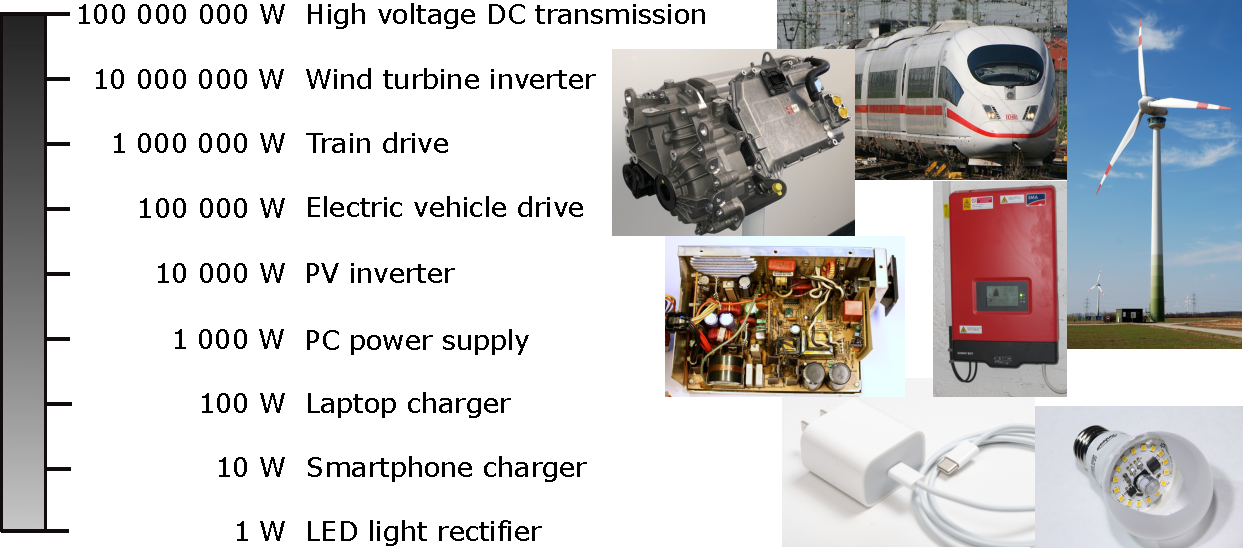
\includegraphics[height=0.7\textheight]{fig/lec01/Power_Classes_Examples.pdf}
		\caption{Power range overview (figure sources: \href{https://commons.wikimedia.org/wiki/File:DB_AG_406_001-8.jpg}{T. Wolf}, \href{https://commons.wikimedia.org/wiki/File:Wind_turbine_with_observation_deck_bruck_an_der_leitha.jpg}{KoeppiK}, \href{https://commons.wikimedia.org/wiki/File:Vitesco_Technologies_EMR3.jpg}{Caprolactam123}, \href{https://commons.wikimedia.org/wiki/File:Installation_of_solar_PV_panels_-_inverter_-_geograph.org.uk_-_2624304.jpg}{D. Hawgood}, \href{https://commons.wikimedia.org/wiki/File:IBM_PC_XT_5160_Power_Supply.jpg}{Mister rf}, \href{https://commons.wikimedia.org/wiki/File:LED-E27-Light-Bulb-1134.jpg}{D.~Tribble} and \href{https://www.rawpixel.com/image/5923136/photo-image-phone-public-domain-white}{rawpixel} under varying CC licenses) }
		\label{Power_Classes_Examples}
	\end{figure}
\end{frame}

%%%%%%%%%%%%%%%%%%%%%%%%%%%%%%%%%%%%%%%%%%%%%%%%%%%%%%%%%%%%%
%% Typical power electronic objectives %%
%%%%%%%%%%%%%%%%%%%%%%%%%%%%%%%%%%%%%%%%%%%%%%%%%%%%%%%%%%%%%
\begin{frame}[c]
	\frametitle{Typical power electronic objectives}
	\begin{figure}
		\begin{tikzpicture}
			\begin{axis}[
				height=.70\textheight,
				ylabel={Efficiency},
				xlabel={Power density},
				zlabel={Costs / ressources},
				xlabel style={sloped},
				ylabel style={sloped}, 
				xticklabel style = {yshift=0.2cm, rotate=25},
				view={70}{25},
				grid,
				ymax = 1,
				xmax = 1,
				zmax = 1,
				xtick distance = 0.25,
				ytick distance = 0.25,
				ztick distance = 0.25
			]
			\addplot3[
				mesh,
				samples=20,
				domain=0:1,
				draw = signalblue
			](
				{sqrt(1-x^2) * cos(deg(y))},
				{sqrt( 1-x^2 ) * sin(deg(y))},
				{x}
			);
			\end{axis}
		\end{tikzpicture}
		\caption{Illustration of typical, conflicting power electronic (normalized) objectives via a Pareto front}
		\label{fig:power_electronic_objectives}
	\end{figure}
\end{frame}

%%%%%%%%%%%%%%%%%%%%%%%%%%%%%%%%%%%%%%%%%%%%%%%%%%%%%%%%%%%%%
%% Subsection: Energy, work, and power %%
%%%%%%%%%%%%%%%%%%%%%%%%%%%%%%%%%%%%%%%%%%%%%%%%%%%%%%%%%%%%%
\subsection{Energy, work, and power}

%%%%%%%%%%%%%%%%%%%%%%%%%%%%%%%%%%%%%%%%%%%%%%%%%%%%%%%%%%%%%
%% Terminology: work vs. energy%%
%%%%%%%%%%%%%%%%%%%%%%%%%%%%%%%%%%%%%%%%%%%%%%%%%%%%%%%%%%%%%
\begin{frame}[c]
	\frametitle{Terminology: work vs. energy}
	\begin{columns}
		\begin{column}{0.5\textwidth}
			\onslide<2->{
				\begin{varblock}{Work}
					Work is the integral of the power over a time integral (or force over distance) and is a measure of the energy transfer.
				\end{varblock}
			}
		\end{column}
		\begin{column}{0.5\textwidth}
			\onslide<1->{
				\begin{varblock}{Energy}
					Energy is the capacity to do work, that is, a quantity depending on the state of a system at a given point of time.				
				\end{varblock}
			}
		\end{column}
	\end{columns}
	\vspace{0.5cm}
	\begin{figure}
		\begin{tikzpicture}
			\onslide<1->{\node[draw, bubble, minimum width = 8em, minimum height = 5em] (energy) at (0,0) {\large Energy};}
			\onslide<3->{
				\coordinate (loss) at (4.5,-1.25);
				\node[draw, bubble] (energy2) at (6,0) {\large Energy};
				}
			\begin{scope}[on background layer]
				\onslide<2->\draw[-{Latex[length=4mm, width=8mm]}, line width=4mm] (energy.mid) -- node[above, midway, name = work] {Work} (energy2);
				\onslide<3->{
					\draw[-{Latex[length=4mm, width=8mm]}, line width=2mm, color=signalred, transform canvas={yshift=-3mm}] (energy.mid) --  (3,0) to [out=0,in=120] (loss.south) ;
					\node[below, transform canvas={yshift=-3mm}] at (loss) {\color{signalred} \large Heat};
					\node[below=of work, yshift = 6mm, color=signalred] {Losses};
				}
			\end{scope}
		\end{tikzpicture}
		\vspace{0.75cm}
		\onslide<3->{\caption{Illustration addressing the work vs. energy terminology (simplified Sankey diagram)}}
		\label{fig:work_vs_energy}
	\end{figure}
\end{frame}

%%%%%%%%%%%%%%%%%%%%%%%%%%%%%%%%%%%%%%%%%%%%%%%%%%%%%%%%%%%%%
%% Power Power balance of an electrical energy conversion system %%
%%%%%%%%%%%%%%%%%%%%%%%%%%%%%%%%%%%%%%%%%%%%%%%%%%%%%%%%%%%%%
\begin{frame}
	\frametitle{Power balance of an electrical energy conversion system}
	\begin{figure}
		\begin{tikzpicture}[auto, node distance = 1.5cm and 2cm]
			\draw
				node [input, name = input] {}
				node [bubble, right = of input, minimum height = 4em] (pc) {\large Power converter}
				node [output, name = output, right = of pc] {}
				node [output, name = losses, below = of pc] {};
				\draw[-{Latex[length=4mm, width=8mm]}, line width=3mm] (input) -- node[below, midway, align=left, name = input2] {Electrical\\input power} (pc);
			\onslide<3->{\node[overlay, bubble, right = of input, minimum height = 4em, pin=80:Change of stored energy $ \frac{\mathrm{d}}{\mathrm{d}t}E_\mathrm{i}(t)$] {\large Power converter};}
			\begin{scope}[on background layer]
				\onslide<4->{\draw[-{Latex[length=4mm, width=8mm]}, line width=3mm] (pc.mid) -- node[below, near end, align=left, name=output2] {Electrical\\output power} (output);}
				\onslide<2->{\draw[-{Latex[length=4mm, width=8mm]}, line width=3mm, color=signalred] (pc.mid) -- node[right, yshift=-2.5mm, name = losses2] {Losses} (losses);}
			\end{scope}
			\onslide<2->{\node[left=of losses2, color=signalred, xshift = 1.8cm] {$P_\mathrm{l}(t)$};}
			\onslide<4->{\node[above=of output2.mid,, align=center, xshift = -0.3cm, yshift = -5mm] {$P_\mathrm{out}(t)$};}
			\node[above=of input2.mid,, align=center, xshift = -0.3cm, yshift = -5mm] {$P_\mathrm{in}(t)$};
		\end{tikzpicture}
		\onslide<4->{\caption{Power balance of an energy conversion system}}
		\label{fig:power_balance_energy_conversion}
	\end{figure}
	\vspace{-0.5cm}
	The \hl{power balance}
	\begin{equation}
		\onslide<1->{P_\mathrm{in}(t)} \onslide<2->{= P_\mathrm{l}(t)}  \onslide<3->{+ \frac{\mathrm{d}}{\mathrm{d}t}E_\mathrm{i}(t)} \onslide<4->{+ P_\mathrm{out}(t)}
	\end{equation}
	must hold for any point in time as energy is conserved, that is, not created or destroyed.
\end{frame}

%%%%%%%%%%%%%%%%%%%%%%%%%%%%%%%%%%%%%%%%%%%%%%%%%%%%%%%%%%%%%
%% Efficiency %%
%%%%%%%%%%%%%%%%%%%%%%%%%%%%%%%%%%%%%%%%%%%%%%%%%%%%%%%%%%%%%
\begin{frame}
	\frametitle{Efficiency}
	\begin{figure}
		\begin{tikzpicture}[auto, node distance = 1.5cm and 2cm]
			\draw
				node [input, name = input] {}
				node [bubble, right = of input, minimum height = 4em] (pc) {\large Power converter}
				node [output, name = output, right = of pc] {}
				node [output, name = losses, below = of pc] {};
			\draw[-{Latex[length=4mm, width=8mm]}, line width=3mm] (input) -- node[below, midway, align=left, name = input2] {Electrical\\input power} (pc);
			\begin{scope}[on background layer]
				\draw[-{Latex[length=4mm, width=8mm]}, line width=3mm] (pc.mid) -- node[below, near end, align=left, name=output2] {Electrical\\output power} (output);
				\draw[-{Latex[length=4mm, width=8mm]}, line width=3mm, color=signalred] (pc.mid) -- node[right, yshift=-2.5mm, name = losses2] {Losses} (losses);
			\end{scope}
			\node[left=of losses2, color=signalred, xshift = 1.8cm] {$P_\mathrm{l}$};
			\node[above=of output2.mid,, align=center, xshift = -0.3cm, yshift = -5mm] {$P_\mathrm{out}$};
			\node[above=of input2.mid,, align=center, xshift = -0.3cm, yshift = -5mm] {$P_\mathrm{in}$};
		\end{tikzpicture}
		\caption{Power balance of an energy conversion system in steady state}
		\label{fig:power_balance_energy_conversion_steady_state}
	\end{figure}
	\vspace{-0.5cm}
	The power balance in \hl{steady state} ($\nicefrac{\mathrm{d}x(t)}{\mathrm{d} t}=0$) is
	\begin{equation}
		P_\mathrm{in} = P_\mathrm{out} + P_\mathrm{l}
	\end{equation}
	\pause
	and leads to the definition of the \hl{efficiency}
	\begin{equation}
		\eta = \frac{P_\mathrm{out}}{P_\mathrm{in}} = \frac{P_\mathrm{out}}{P_\mathrm{out} + P_\mathrm{l}}.
	\end{equation}
\end{frame}

%%%%%%%%%%%%%%%%%%%%%%%%%%%%%%%%%%%%%%%%%%%%%%%%%%%%%%%%%%%%%
%% Four quadrants of operation %%
%%%%%%%%%%%%%%%%%%%%%%%%%%%%%%%%%%%%%%%%%%%%%%%%%%%%%%%%%%%%%
\begin{frame}
	\frametitle{Four quadrants of operation}
	\begin{columns}
		\begin{column}{0.5\textwidth}
			\justifying
			\onslide<1->{%
				Depending on the current and voltage signs, the power $P$ can be positive or negative. This leads to four \hl{quadrants} of operation:%
			}%
			\begin{itemize}
				\item<2-> Quadrants I \& III: $P \geq 0$,\newline (Power transfer from input to output)
				\item<3-> Quadrants II \& IV: $P \leq 0$. \newline (Power transfer from output to input)
			\end{itemize}
			\onslide<4->{
				How many quadrants a power converter can operate in depends on the topology and control strategy, i.e., is an important design criterion.
				}
		\end{column}
		\begin{column}{0.5\textwidth}
			\begin{figure}
				\centering
				\begin{tikzpicture}
					\onslide<1->{
						\draw[<->] (-2,0) -- (2,0) node[anchor=west] {$i$};
						\draw[<->] (0,-2) -- (0,2) node[anchor=south] {$u$};
					}
					\onslide<2->{\node[anchor=center, align = center] at (1.0,1.0) {$\mathrm{I}$\\$P \geq 0$};}
					\onslide<3->{\node[anchor=center, align = center] at (-1.0,1.0) {$\mathrm{II}$\\$P \leq 0$};}
					\onslide<2->{\node[anchor=center, align = center] at (-1.0,-1.0) {$\mathrm{III}$\\$P \geq 0$};}
					\onslide<3->{\node[anchor=center, align = center] at (1.0,-1.0) {$\mathrm{IV}$\\$P \leq 0$};}
					\node[anchor = center, xshift = 1mm] at (0, 3.5) {
						\begin{circuitikz}
							\node[twoportsplitshape, scale = 1.5](tp){};
							\draw (tp.left up) to [short, -o, i_<= $i_1$] ++(-0.75,0) coordinate(tpin1)
							(tp.left down) to [short, -o] ++(-0.75,0) coordinate(tpin2);
							\draw[->] ([xshift=-0.9cm]tp.left up) to node[anchor = east]{$u_1$} ([xshift=-0.9cm]tp.left down);
							\draw (tp.right up) to [short, -o, i= $i_2$] ++(0.75,0) coordinate(tpout1)
							(tp.right down) to [short, -o] ++(+0.75,0) coordinate(tpout2);
							\draw[->] ([xshift=1cm]tp.right up) to node[anchor = west]{$u_2$} ([xshift=1cm]tp.right down);
						\end{circuitikz}	
					} ;
				\end{tikzpicture}
				\caption{Four quadrants of energy conversion}
				\label{fig:four_quadrants}
			\end{figure}
		\end{column}
	\end{columns}
\end{frame}

%%%%%%%%%%%%%%%%%%%%%%%%%%%%%%%%%%%%%%%%%%%%%%%%%%%%%%%%%%%%%
%% Why efficiency matters: a computer supply example %%
%%%%%%%%%%%%%%%%%%%%%%%%%%%%%%%%%%%%%%%%%%%%%%%%%%%%%%%%%%%%%
\begin{frame}[c]
	\frametitle{Why efficiency matters: a computer supply example}
	\begin{table}
		\centering
		\begin{tabular}{lcc}
			\toprule
			& Power supply A & Power supply B \\
			& 80 PLUS Gold & 80 PLUS Titanium \\
			\midrule
			Input power & \multicolumn{2}{c}{\SI{250}{\watt}} \pause\\
			Efficiency & \SI{89}{\percent} & \SI{94}{\percent}  \pause\\
			Power loss & \SI{27.5}{\watt} & \SI{15}{\watt} \pause\\
			\midrule
			Operating hours per year & \multicolumn{2}{c}{$\SI{8}{\hour} \times 220 = \SI{1760}{\hour}$} \pause\\
			Cumulated power loss per year & \SI{48.4}{\kilo\watt\hour} & \SI{26.4}{\kilo\watt\hour} \pause\\
			Electricity cost for yearly power losses & \SI{14.52}{\EUR} & \SI{7.92}{\EUR} \pause\\
			\midrule
			Cumulated power loss in Germany & \SI{1.936}{\tera\watt\hour} & \SI{1.056}{\tera\watt\hour} \pause\\
			Electricity cost for power loss in Germany & \SI{580.8}{\mega\EUR} & \SI{316.8}{\mega\EUR} \\
			\bottomrule
		\end{tabular}
		\label{tab:efficiency_computer_supply_example}
		\caption{Comparison of two computer power supplies (further assumptions: effective nominal power calculation, electricity price \SI[fraction-function=\nicefrac]{0.3}{\EUR\per\kilo\watt\per\hour}, $40\cdot 10^6$ computers in Germany)}
	\end{table}
\end{frame}

%%%%%%%%%%%%%%%%%%%%%%%%%%%%%%%%%%%%%%%%%%%%%%%%%%%%%%%%%%%%%
%% Why efficiency matters: a wind power plant example %%
%%%%%%%%%%%%%%%%%%%%%%%%%%%%%%%%%%%%%%%%%%%%%%%%%%%%%%%%%%%%%
\begin{frame}[c]
	\frametitle{Why efficiency matters: a wind power plant example}
	\begin{table}
		\centering
		\begin{tabular}{lcc}
			\toprule
			& Wind power plant A & Wind power plant B \\
			\midrule
			Input power & \multicolumn{2}{c}{\SI{5}{\mega\watt}} \pause\\
			Efficiency & \SI{97}{\percent} & \SI{97.1}{\percent}  \pause\\
			Power loss & \SI{150}{\kilo\watt} & \SI{145}{\kilo\watt}\pause\\
			\midrule
			Nominal power operating hours per year & \multicolumn{2}{c}{$\SI{3000}{\hour}$} \pause\\
			Cumulated power loss per year & \SI{450}{\mega\watt\hour} & \SI{435}{\mega\watt\hour} \pause\\
			Cumulated power loss (lifetime) & \SI{9.0}{\giga\watt\hour} & \SI{8.7}{\giga\watt\hour} \pause\\
			\midrule
			Lost sales proceeds due to losses per year  & \SI{22.5}{\kilo\EUR} & \SI{21.75}{\kilo\EUR} \pause\\
			Lost sales proceeds due to losses (lifetime)  & \SI{450}{\kilo\EUR} & \SI{435}{\kilo\EUR} \pause\\
			\midrule
			Cumulated power loss (lifetime, Germany)  & \SI{9.0}{\tera\watt\hour} & \SI{8.7}{\tera\watt\hour} \pause\\
			Lost sales proceeds (lifetime, Germany)  & \SI{450}{\mega\EUR} & \SI{435}{\mega\EUR} \\
			\bottomrule
		\end{tabular}
		\label{tab:efficiency_wind_power_example}
		\caption{Comparison of two wind power plants (further assumptions:  electricity sales price \SI[fraction-function=\nicefrac]{0.05}{\EUR\per\kilo\watt\per\hour}, $20$ years of life time, $\num{1000}$ newly constructed wind power plants per year in Germany)}
	\end{table}
\end{frame}

%%%%%%%%%%%%%%%%%%%%%%%%%%%%%%%%%%%%%%%%%%%%%%%%%%%%%%%%%%%%%
%% Subsection: Linear vs. switched power conversion %%
%%%%%%%%%%%%%%%%%%%%%%%%%%%%%%%%%%%%%%%%%%%%%%%%%%%%%%%%%%%%%
\subsection{Linear vs. switched power conversion}

%%%%%%%%%%%%%%%%%%%%%%%%%%%%%%%%%%%%%%%%%%%%%%%%%%%%%%%%%%%%%
%% Linear power conversion %%
%%%%%%%%%%%%%%%%%%%%%%%%%%%%%%%%%%%%%%%%%%%%%%%%%%%%%%%%%%%%%
\begin{frame}[c]
	\frametitle{Linear power conversion}
	\begin{figure}
		\begin{circuitikz}[]
			\draw (0,2) to [open, o-o, v = $\hspace{2cm}u_2(t)$, voltage = straight] ++(0,-2)
			to ++(-6,0)
			to [open, o-o, v<= $u_1(t) \hspace{2cm}$, voltage = straight] ++(0,2)
			to [european resistor, R=$R_1$] ++(4,0) 
			to ++(2,0)
			(-2,0) to [variable european resistor, *-*, l=$R_2$] (-2,2);
		\end{circuitikz}
		\caption{Adjustable resistive voltage divider as step-down converter}
		\label{fig:linear_power_conversion}
	\end{figure}
	\pause
	With Kirchhoff's voltage law, the output voltage $u_2(t)$ is
	\begin{equation}
		u_2(t) = u_1(t) \frac{R_2}{R_1 + R_2}.
	\end{equation}
	\pause
	By adjusting the resistance $R_2$, the output voltage can be controlled. However, this method is \hl{inefficient} as the power loss is independent of the output power and given by
	\begin{equation}
		P_\mathrm{l}(t) = \frac{u_1^2(t)}{R_1 + R_2}.
	\end{equation}
\end{frame}

%%%%%%%%%%%%%%%%%%%%%%%%%%%%%%%%%%%%%%%%%%%%%%%%%%%%%%%%%%%%%
%% Linear power conversion (cont.) %%
%%%%%%%%%%%%%%%%%%%%%%%%%%%%%%%%%%%%%%%%%%%%%%%%%%%%%%%%%%%%%
\begin{frame}[c]
	\frametitle{Linear power conversion (cont.)}
	\begin{columns}
		\begin{column}{0.55\textwidth}
			\begin{figure}
				\onslide<1->{
				\begin{circuitikz}[]
					\draw (0,2) to [open, o-o, v = $\hspace{2cm}u_2(t)$, voltage = straight] ++(0,-2)
					to ++(-5.5,0)
					to [open, o-o, v<= $u_1(t) \hspace{2cm}$, voltage = straight] ++(0,2)
					(-5.5,2) to ++(1.25,0) node [nigbt, anchor=C, rotate=90](nigbt1){}
					(nigbt1.E) to [short, i=$i_2(t)$] (0,2);
					\draw node[rectangle, draw, anchor = north] (r) at (nigbt1.B) {Linear amplifier}
						(r.east)[<-] to ++(0.5,0) node [anchor = west](a){$u^*_2(t)$};
					\draw [->] ([yshift = 0.2cm, xshift = 0.1cm]nigbt1.C) -- node [yshift = 0.3cm] {$u_\mathrm{CE}(t)$} ([yshift = 0.2cm, xshift = -0.1cm]nigbt1.E) ;  
				\end{circuitikz}
				\caption{Transistor-based step-down converter}
				\label{fig:linear_power_conversion_transistor}
				}
			\end{figure}
			\onslide<3->{
			For a transistor-based step-down converter, the output voltage  is $u_2(t)= u_1(t) - u_\mathrm{CE}(t)$	leading to the power losses
			\begin{equation}
				P_\mathrm{l}(t) = u_\mathrm{CE}(t)  i_2(t) .
			\end{equation}
			}
		\end{column}
		\begin{column}{0.45\textwidth}
			\centering
			\begin{figure}
				\onslide<2->{
				\begin{tikzpicture}
					% plot IGBT output characteristics V_CE = f(I_C)
					\begin{axis}[
						xlabel={$U_{\mathrm{CE}}$},
						ylabel={$I_\mathrm{C}$},
						axis lines=left,
						ymin=0, ymax=6,
						xmin=0, xmax=5,
						xtick={0,1,2,3,4},
						ytick={0,1,2,3,4,5},
						%no x/y ticks displayed
						xticklabels={},
						yticklabels={},
						domain=0:5,
						samples=50,
						thick,
						smooth,
						no markers,
						width = 0.95\textwidth,
						grid
						]
						\addplot[signalblue, domain=0:0.3]{0.01};
						\addplot[signalblue, domain=0.3:5]{11.5 / (1+exp(-2*(x-0.3)))-6};
						\addplot[signalblue, domain=0.3:5]{7.7 / (1+exp(-2.5*(x-0.3)))-4};
						\addplot[signalblue, domain=0.3:5]{4 / (1+exp(-3*(x-0.3)))-2};
						\addplot[signalblue, domain=0.3:5]{2 / (1+exp(-3.25*(x-0.3)))-1};
						\addplot[signalblue, domain=0.3:5]{1 / (1+exp(-3.5*(x-0.325)))-0.5};
						\addplot[signalblue, domain=0.3:5]{0.25 / (1+exp(-3.5*(x-0.325)))-0.125};
						\draw[->, signalbrown, thick, dashed] (axis cs:1.5,0.25) -- (axis cs:1.5,5.2);
						\node[signalbrown, anchor = west] at (axis cs:1.5,2.75) {$U_\mathrm{GE}$};
						\draw[signalgreen, thick, dashed, rotate=-10] (axis cs:0.5,1) ellipse (0.35cm and 3.0cm);
						\node[signalgreen, anchor = south] at (axis cs:1.1,5.1) {\small Linear region};
						\draw[signalred, thick, dashed, rounded corners] (axis cs:2.5,0.2) rectangle (axis cs:4.75,5.9);
						\node[signalred, anchor = south, ,  align=center] at (axis cs:3.6,3.7) {\small Saturation\\region};
					\end{axis}
				\end{tikzpicture}
				\caption{Output characteristics of an insulated-gate bipolar transistor (IGBT)}
				\label{fig:output_characteristics_IGBT}
				}
			\end{figure}
			\end{column}
	\end{columns}
\end{frame}

%%%%%%%%%%%%%%%%%%%%%%%%%%%%%%%%%%%%%%%%%%%%%%%%%%%%%%%%%%%%%
%% Switching power conversion %%
%%%%%%%%%%%%%%%%%%%%%%%%%%%%%%%%%%%%%%%%%%%%%%%%%%%%%%%%%%%%%
\begin{frame}[b]
	\frametitle{Switching power conversion}
	\onslide<1->{Alternative idea: \hl{switch either fully on or off}.} \onslide<3->{The average output voltage $\overline{u}_2$ is controlled by the \hl{duty cycle} (assuming that $u_1(t)=\overline{u}_1$ is constant)
	\begin{equation}
		D = \frac{T_\mathrm{on}}{T_\mathrm{s}}, \qquad \overline{u}_2 = \frac{1}{T_\mathrm{s}} \int_0^{T_\mathrm{s}} u_2(t) \mathrm{d}t = D \overline{u}_1.
	\end{equation}}
	\onslide<4->{%
		As the switching losses are typically small, the overall efficiency is (much) higher compared to linear power conversion.} 
	\vspace{-0.5cm}  
	\begin{columns}[b]
		\begin{column}{0.5\textwidth}
			\begin{figure}
				\onslide<1->{
				\begin{circuitikz}[]
					\draw (0,2) to [open, o-o, v = $\hspace{2cm}u_2(t)$, voltage = straight] ++(0,-2)
					to ++(-5,0)
					to [open, o-o, v<= $u_1(t) \hspace{2cm}$, voltage = straight] ++(0,2)
					(-5,2) to ++(1.25,0) node [cuteopenswitchshape, anchor = out, rotate=180] (S) {}
					let \p1 = (S.mid) in (S.in) to (0,2)
					([yshift = -0.3cm]S.mid) to [short, o-*](\x1,0);
				\end{circuitikz}
				\vspace{0.6cm}
				\caption{Ideal switch-based step-down converter}
				\label{fig:Switched_power_conversion}
				}
			\end{figure}
			\vspace{0pt}
		\end{column}
		\begin{column}{0.5\textwidth}
			\centering
			\begin{figure}
				\onslide<2->{
				\begin{tikzpicture}
					\begin{axis}[
						xlabel={$t/T_\mathrm{s}$},
						ylabel={$u_2(t)/u_1(t)$},
						ymin=-0.05, ymax=1.05,
						xmin=-0.1, xmax=1.1,
						width = 0.95\textwidth,
						height = 0.4\textheight,
						grid,
						thick,
						clip = false,
						]
						% plt u_out = 1 for t = 0 to D*Ts and u_out = 0 for t = D*Ts to Ts in a single plot
						\addplot[signalblue] coordinates {(-0.1,0) (0,0) (0,1) (0.4,1) (0.4,0) (1,0) (1,1) (1.1,1)};
						\draw [thick,<->]  (0,0.5) -- node[above,fill=white]{$T_\mathrm{on}$}(0.4, 0.5); 
						\draw [thick,<->]  (0.4,0.5) -- node[above]{$T_\mathrm{off}$}(1.0, 0.5);
						\draw [thick,<->]  (0.0,1.2) -- node[above]{$T_\mathrm{s}$}(1.0, 1.2); 
					\end{axis}
				\end{tikzpicture}
				\caption{Switching output voltage from \figref{fig:Switched_power_conversion}}
				\label{fig:Switched_power_conversion_output}
				}
			\end{figure}
			\vspace{0pt}
			\end{column}
	\end{columns}
\end{frame}

%%%%%%%%%%%%%%%%%%%%%%%%%%%%%%%%%%%%%%%%%%%%%%%%%%%%%%%%%%%%%
%% Switching power conversion %%
%%%%%%%%%%%%%%%%%%%%%%%%%%%%%%%%%%%%%%%%%%%%%%%%%%%%%%%%%%%%%
\begin{frame}
	\frametitle{Switching power conversion: switching losses}
	\begin{columns}[b]
		\begin{column}{0.3\textwidth}
			Switching process is not free of power loss:
			$$\overline{P}_\mathrm{l} = \frac{1}{T_\mathrm{s}} \int_0^{T_\mathrm{s}} u_\mathrm{s}(t) i_\mathrm{s}(t) \mathrm{d}t .$$
			\vspace{-0.6cm}
			\begin{figure}
				\begin{circuitikz}[]
					\draw (0,1.5) to [vsource, v=$u_0$, name=vs] (0,0)
					to (1.5,0) [short]
					to ++(0,0.5) node [cspstshape, anchor = right, rotate = -90] (S) {};
					\draw (S.left) to ++(0,0.5)  [short, -*] coordinate (S1);
					\draw (S1) to [diode] ++(0,2) coordinate (S3)
					to ++(1,0) [short]	coordinate (S2)
					to  [isource, i=$i_0$] ++(0, -2.0)
					to  [short, -*] (S1);
					\draw (S3) to [short, *-] ++(-1.5,0)
					to (vs) [short];
					\draw (S.right) to [short, i=$i_\mathrm{s}$] ++(0,-0.5); 
					\draw [->] ([xshift = 0.45cm, yshift=0.1cm]S.left) -- node [xshift = 0.45cm] {$u_\mathrm{s}$} ([xshift = 0.45cm, yshift =-0.1cm]S.right);
				\end{circuitikz}
				\caption{Idealized switching loss model}
				\label{fig:idealized_switch_model}
			\end{figure}
			\pause
		\end{column}
		\begin{column}{0.7\textwidth}
			\centering
			\begin{figure}
				\begin{tikzpicture}
					\begin{groupplot}[group style={group size=1 by 3}, height=0.34\textheight, width=0.875\textwidth, xmin=-0.1, xmax=1.1, grid,clip = false, ymin = -0.1, ymax =1.1]

					% Top plot: switch control signal
					\nextgroupplot[ylabel = {$u_\mathrm{ctrl}(t)$}, ytick = {0, 0.5, 1}, yticklabels = {off, , on}]
						\addplot[signalblue, thick] coordinates {(-0.1,0) (0,0) (0,1) (0.5,1) (0.5,0) (1,0) (1,1) (1.1,1)};
						\draw [thick,<->]  (0,0.4) -- node[above, fill=white, inner sep = 1pt]{$T_\mathrm{on}$}(0.5, 0.4); 
						\draw [thick,<->]  (0.5,0.4) -- node[above, fill=white, inner sep = 1pt]{$T_\mathrm{off}$}(1.0, 0.4);
						
						% Middle plot: voltage and current through a switch (two y-axes)
						\nextgroupplot[ylabel = {$u_\mathrm{s}(t)/u_0$}]
							\addplot[signalblue, thick] coordinates {(-0.1,1) (0,1) (0.1,0) (0.5,0) (0.6,1) (1,1) (1.1,1)};
							\draw[{Latex[length=2mm]}-, thin, signalblue] (axis cs:0.6,0.9) -- node[right=1mm, fill=white, inner sep = 1pt]{$u_\mathrm{s}(t)$}(axis cs:0.75,0.5);
							\draw[{Latex[length=2mm]}-, thin, signalred] (axis cs:0.8,0.1) -- node[right=1mm, fill=white, inner sep = 1pt]{$i_\mathrm{s}(t)$}(axis cs:0.95,0.5);
						
						% Bottom plot: power loss in the switch
						\nextgroupplot[xlabel = {$t/T_\mathrm{s}$}, ylabel = {$P_\mathrm{l}(t)/P_\mathrm{max}$}]
							\addplot[signalblue, domain = -0.1:0, thick] {0};
							\addplot[signalblue, domain = 0.0:0.1, thick,fill=signalblue, 
							fill opacity=0.1] {-(x-0.05)^2/(0.05)^2+1};
							\addplot[signalblue, domain = 0.5:0.6, thick,fill=signalblue, 
							fill opacity=0.1] {-(x-0.55)^2/(0.05)^2+1};
							\addplot[signalblue, domain = 0.1:0.5, thick] {0};
							\addplot[signalblue, domain = 0.6:1.1, thick] {0};
							% add textbox with arrow pointing towards the first power loss curve
							\draw[{Latex[length=2mm]}-, thin, signalblue] (axis cs:0.05,0.4) -- node[right=1mm, fill=white, inner sep = 1pt]{$E_\mathrm{on}$}(axis cs:0.25,0.5);
							\draw[{Latex[length=2mm]}-, thin, signalblue] (axis cs:0.55,0.4) -- node[right=1mm, fill=white, inner sep = 1pt]{$E_\mathrm{off}$}(axis cs:0.75,0.5);
						
					\end{groupplot}
					% second y-axis for the middle plot
					\begin{groupplot}[group style={group size=1 by 3, y descriptions at = edge right}, height=0.34\textheight, width=0.875\textwidth, xmin=-0.1, xmax=1.1, grid,clip = false, xtick=\empty, axis line style=transparent, ymin = -0.1, ymax =1.1]
						\nextgroupplot[ytick = \empty]
							%
						\nextgroupplot[ylabel = {$i_\mathrm{s}(t)/i_0$}, ytick = {}, yticklabels = {}]
							\addplot[signalred, thick] coordinates {(-0.1,0) (0,0) (0.1,1) (0.5,1) (0.6,0) (1,0) (1.1,0)};
							\addplot[signalblue, thick] coordinates {(-0.1,1) (0,1) (0.1,0) (0.5,0) (0.6,1) (1,1) (1.1,1)}; %plot second time to prevent overlap from grid lines
						\nextgroupplot[ytick = \empty]
							%
					\end{groupplot}
				%	
				\end{tikzpicture}
			\end{figure}
			\end{column}
	\end{columns}
\end{frame}

%%%%%%%%%%%%%%%%%%%%%%%%%%%%%%%%%%%%%%%%%%%%%%%%%%%%%%%%%%%%%
%% Switching power conversion %%
%%%%%%%%%%%%%%%%%%%%%%%%%%%%%%%%%%%%%%%%%%%%%%%%%%%%%%%%%%%%%
\begin{frame}[b]
	\frametitle{Switching power conversion: soft switching}
	\begin{figure}
		\onslide<1->{
		\begin{subfigure}[b]{0.44\textwidth}
			\hspace{-0.7cm}
			\begin{tikzpicture}
				\begin{groupplot}[group style={group size=1 by 2}, height=0.34\textheight, width=\textwidth, xmin=0, xmax=1, grid, ymin = -0.1, ymax =1.1]
	
				% Top-left plot: switch control signal for ZVS
				
				\nextgroupplot[ylabel = {$u_\mathrm{ctrl}(t)$}, ytick = {0, 0.5, 1}, yticklabels = {off, , on}]
					\addplot[signalblue, thick] coordinates {(-0.1,0) (0.3,0) (0.3,1) (0.7,1) (0.7,0) (1.1,0)};
					\coordinate (a) at (0.3,0);
					\coordinate (b) at (0.7,0);
					
	
				% Bottom-left plot: voltage and current through a switch for ZVS
				\nextgroupplot[ylabel = {$u_\mathrm{s}(t)/u_0$}]
					\addplot[signalblue, thick] coordinates {(0,1) (0.2,1) (0.3,0) (0.7,0) (0.8,1) (1,1)};
					\node[signalred, fill=white, inner sep = 1pt, anchor = north] at (axis cs:0.5,1) {$i_\mathrm{s}(t)$};
					\node[signalblue, fill=white, inner sep = 1pt, anchor = south] at (axis cs:0.5,0) {$u_\mathrm{s}(t)$};
					\coordinate (c) at (0.3,0);
					\coordinate (d) at (0.7,0);
				\end{groupplot}

				% second y-axis for the bottom plot
				\begin{groupplot}[group style={group size=1 by 2, y descriptions at = edge right}, height=0.34\textheight, width=\textwidth, xmin=0, xmax=1, grid, xtick=\empty, axis line style=transparent, ymin = -0.1, ymax =1.1]
					\nextgroupplot[ytick = \empty]
					%
					\nextgroupplot[ylabel = {$i_\mathrm{s}(t)/i_0$}, ytick = {}, yticklabels = {}]
						\addplot[signalred, thick] coordinates {(0,0) (0.25,0) (0.35,1) (0.65,1) (0.75,0) (1,0)};
						\addplot[signalblue, thick] coordinates {(0,1) (0.2,1) (0.3,0) (0.7,0) (0.8,1) (1,1)};
				\end{groupplot}
				\draw [dashed] (a) -- (c);
                \draw [dashed] (b) -- (d);
			\end{tikzpicture}
			\caption{Zero-voltage switching (ZVS)}
		\end{subfigure}
		}
		%
		\hspace{0.5cm}
		%
		\onslide<2->{
		\begin{subfigure}[b]{0.44\textwidth}
		\begin{tikzpicture}
			\begin{groupplot}[group style={group size=1 by 2}, height=0.34\textheight, width=\textwidth, xmin=0, xmax=1, grid, ymin = -0.1, ymax =1.1]
	
				% Top-right plot: switch control signal for ZVS
				\nextgroupplot[ylabel = {$u_\mathrm{ctrl}(t)$}, ytick = {0, 0.5, 1}, yticklabels = {off, , on}]
					\addplot[signalblue, thick] coordinates {(-0.1,0) (0.3,0) (0.3,1) (0.7,1) (0.7,0) (1.1,0)};
					\coordinate (a) at (0.3,0);
					\coordinate (b) at (0.7,0);
				
				% Bottom-right plot: voltage and current through a switch for ZCS
				\nextgroupplot[ylabel = {$u_\mathrm{s}(t)/u_0$}]
					\addplot[signalblue, thick] coordinates {(0,1) (0.25,1) (0.35,0) (0.65,0) (0.75,1) (1,1)};
					\node[signalred, fill=white, inner sep = 1pt, anchor = north] at (axis cs:0.5,1) {$i_\mathrm{s}(t)$};
					\node[signalblue, fill=white, inner sep = 1pt, anchor = south] at (axis cs:0.5,0) {$u_\mathrm{s}(t)$};
					\coordinate (c) at (0.3,0);
					\coordinate (d) at (0.7,0);
				\end{groupplot}

				% second y-axis for the bottom plot
				\begin{groupplot}[group style={group size=1 by 2, y descriptions at = edge right}, height=0.34\textheight, width=\textwidth, xmin=0, xmax=1, grid, xtick=\empty, axis line style=transparent, ymin = -0.1, ymax =1.1]
					\nextgroupplot[ytick = \empty]
					%
					\nextgroupplot[ylabel = {$i_\mathrm{s}(t)/i_0$}, ytick = {}, yticklabels = {}]
						\addplot[signalred, thick] coordinates {(0,0) (0.3,0) (0.4,1) (0.6,1) (0.7,0) (1,0)};
						\addplot[signalblue, thick] coordinates {(0,1) (0.25,1) (0.35,0) (0.65,0) (0.75,1) (1,1)};
					%
				\end{groupplot}
				\draw [dashed] (a) -- (c);
                \draw [dashed] (b) -- (d);
		\end{tikzpicture}
		\caption{Zero-current switching (ZCS)}
	\end{subfigure}
		
		\caption{Soft switching: reducing switching losses by turning on or off the switch when it does not transfer any power (note: above's voltage and current shapes are heavily idealized and require an appropriate circuit design besides the actual switch to enable soft switching)}
		\label{fig:soft_switching}}
	\end{figure}
\end{frame}

%%%%%%%%%%%%%%%%%%%%%%%%%%%%%%%%%%%%%%%%%%%%%%%%%%%%%%%%%%%%%
%% Switching power conversion: passive components as filters / energy buffers %%
%%%%%%%%%%%%%%%%%%%%%%%%%%%%%%%%%%%%%%%%%%%%%%%%%%%%%%%%%%%%%
\begin{frame}[c]
	\frametitle{Switching power conversion: passive components as filters / energy buffers}
	
	\begin{figure}
	\centering
				\begin{tikzpicture}[ampersand replacement=\&]
					
					\node[] (A) at (0,0) {
						\begin{circuitikz}[]
							\draw (0,2) to [open, o-o, v = $\hspace{2cm}u_2(t)$, voltage = straight] ++(0,-2)
							to ++(-6,0)
							to [open, o-o, v<= $u_1(t) \hspace{2cm}$, voltage = straight] ++(0,2)
							(-6,2) to ++(1.25,0) node [cuteopenswitchshape, anchor = out, rotate=180] (S) {}
							let \p1 = (S.mid) in (S.in) to [inductor, l_=$L$] (0,2) 
							([yshift = -0.3cm]S.mid) to [short, o-*](\x1,0);
							\draw (-0.75,2) to [capacitor, *-*, l_=$C$] (-0.75,0);
							\draw (-3.5,2) to [open, v = $\hspace{1.75cm}u_\mathrm{s}(t)$, voltage = straight] ++(0,-2);
						\end{circuitikz}
					};
					\pause	
					\matrix [anchor = north, column sep = 1cm] at (0,-1.5){
						\begin{axis}[
							xlabel={$t/T_\mathrm{s}$},
							ylabel={$u_\mathrm{s}(t)/u_1(t)$},
							ymin=-0.05, ymax=1.05,
							xmin=-0.1, xmax=1.1,
							width = 0.45\textwidth,
							height = 0.4\textheight,
							grid,
							thick,
							clip = false,
							]
							% plt u_out = 1 for t = 0 to D*Ts and u_out = 0 for t = D*Ts to Ts in a single plot
							\addplot[signalblue] coordinates {(-0.1,0) (0,0) (0,1) (0.4,1) (0.4,0) (1,0) (1,1) (1.1,1)};
							\draw [thick,<->]  (0,0.5) -- node[above,fill=white]{$T_\mathrm{on}$}(0.4, 0.5); 
							\draw [thick,<->]  (0.4,0.5) -- node[above]{$T_\mathrm{off}$}(1.0, 0.5);
							\draw [thick,<->]  (0.0,1.2) -- node[above]{$T_\mathrm{s}$}(1.0, 1.2); 
						\end{axis}
						
						\&

						\begin{axis}[
							xlabel={$t/T_\mathrm{s}$},
							ylabel={$u_2(t)/u_1(t)$},
							ymin=-0.05, ymax=1.05,
							xmin=-0.1, xmax=1.1,
							width = 0.45\textwidth,
							height = 0.4\textheight,
							grid,
							thick,
							clip = false,
							]
							\addplot[signalblue, dashed] coordinates {(-0.1,0.4) (1.1,0.4)};
							\addplot[dashed] coordinates {(-0.1,0.5) (1.1,0.5)};
							\addplot[dashed] coordinates {(-0.1,0.25) (1.1,0.25)};
							\addplot[signalblue, domain=0:0.4]{0.25 + (x-0.2)^2*0.15/(0.2)^2};
							\addplot[signalblue, domain=0.4:1.0]{0.5 - (x-0.7)^2*0.1/(0.3)^2};
							\addplot[signalblue, domain=-0.1:0]{0.5 - (x+0.3)^2*0.1/(0.3)^2};
							\addplot[signalblue, domain=1.0:1.1]{0.25 + (x-1.2)^2*0.15/(0.2)^2};
							\draw [thick,<->, anchor = mid]  (0,0.8) -- node[midway,fill=white,inner sep = 1pt]{$T_\mathrm{on}$}(0.4, 0.8); 
							\draw [thick,<->, anchor = mid]  (0.4,0.8) -- node[midway,fill=white,inner sep = 1pt]{$T_\mathrm{off}$} (1.0, 0.8);
							\draw [thick,<->]  (0.0,1.2) -- node[above]{$T_\mathrm{s}$}(1.0, 1.2); 
							\draw[-{Latex[length=2mm]}] (0.4, 0.7) -- (0.4, 0.5);
							\draw[-{Latex[length=2mm]}] (0.4, 0.05) -- node[left=1mm, fill=white, inner sep = 1pt, yshift=-0.5mm]{$\Delta u$}(0.4, 0.25);
							\draw[-{Latex[length=2mm]}, thin, signalblue] (0.7, 0.05) -- node[right=1mm, fill=white, inner sep = 1pt, yshift=-2mm]{$\overline{u}_2$}(0.6, 0.4);
						\end{axis}
						\\
						};	
				\end{tikzpicture}
				\caption{Exemplary voltage signals for a switched power conversion system with output filter} 
				\label{fig:Switched_power_conversion_filters}
			\end{figure}
\end{frame}

%%%%%%%%%%%%%%%%%%%%%%%%%%%%%%%%%%%%%%%%%%%%%%%%%%%%%%%%%%%%%
%% Feasible and infeasible filter topologies %%
%%%%%%%%%%%%%%%%%%%%%%%%%%%%%%%%%%%%%%%%%%%%%%%%%%%%%%%%%%%%%
\begin{frame}[c]
	\frametitle{Feasible and infeasible filter topologies}
	\begin{figure}
		\centering	
		\begin{subfigure}{0.45\textwidth}
			\centering
			\begin{circuitikz}[]
				\draw (0,2) to [open, o-o, v = $ $, voltage = straight] ++(0,-2)
				to ++(-5,0)
				to [open, o-o, v<= $ $, voltage = straight] ++(0,2)
				(-5,2) to ++(2,0) node [cuteopenswitchshape, anchor = out, rotate=180] (S) {}
				let \p1 = (S.mid) in (S.in) to [inductor] (0,2) 
				([yshift = -0.3cm]S.mid) to [short, o-*](\x1,0);
				\draw (-4,2) to [capacitor, *-*] (-4,0);
			\end{circuitikz}
			\caption{Feasible filter topology}
		\end{subfigure}%
		\pause
		\begin{subfigure}{0.45\textwidth}
			\centering
			\begin{circuitikz}[]
						\draw (0,2) to [open, o-o, v = $ $, voltage = straight] ++(0,-2)
						to ++(-5,0)
						to [open, o-o, v<= $ $, voltage = straight] ++(0,2)
						(-5,2) to [inductor, name = L1] ++(2,0) node [cuteopenswitchshape, anchor = out, rotate=180] (S) {}
						let \p1 = (S.mid) in (S.in) to [short] (0,2) 
						([yshift = -0.3cm]S.mid) to [short, o-*](\x1,0);
						\draw (-1,2) to [capacitor, *-*, name = C1] (-1,0);
						\node[correct forbidden sign, line width = 0.6ex, draw = signalred, minimum size = 1.3cm] at (C1){};
						\node[correct forbidden sign, line width = 0.65ex, draw = signalred, minimum size = 1.3cm] at (L1){};
			\end{circuitikz}
			\caption{Infeasible filter topology}
		\end{subfigure}
	\caption{Basic filter topologies for switched power conversion} 
	\label{fig:Switched_power_conversion_filters_basic}
	\end{figure}
	\pause
	\vspace{-0.25cm}
	\begin{varblock}{Short and open circuit situations}
		\setbeamertemplate{itemize/enumerate body end}{\vspace{0em}}
		Prevent the following situations as they can lead to sparkover and damage:
		\begin{itemize}
			\item Short circuit of capacitor: current peak, 
			\item Open circuit of inductor: voltage peak.
		\end{itemize}
	\end{varblock}

\end{frame}

%%%%%%%%%%%%%%%%%%%%%%%%%%%%%%%%%%%%%%%%%%%%%%%%%%%%%%%%%%%%%
%% Important power electronic devices and idealized characteristics %%
%%%%%%%%%%%%%%%%%%%%%%%%%%%%%%%%%%%%%%%%%%%%%%%%%%%%%%%%%%%%%
\begin{frame}[c]
	\frametitle{Important power electronic devices and idealized characteristics}
	\begin{table}
		\centering
		\begin{tabular}{M{0.22\textwidth} M{0.22\textwidth} M{0.22\textwidth} M{0.22\textwidth}}
			\onslide<1->{Diode} & \onslide<2->{Thyristor} & \onslide<3->{TRIAC (triode for alternating current)} & \onslide<4->{GTO (gate turn-off thyristor)}\\

			\onslide<1->{
			\begin{circuitikz}
				\draw (0,0) to [diode, v=$u$, i=$i$, voltage = straight] (2,0);
			\end{circuitikz}
			}

			&
			\onslide<2->{
			\begin{circuitikz}
				\draw (0,0) to [thyristor, v=$u$, i=$i$, voltage = straight] (2,0);
			\end{circuitikz}
			}
			
			&
			\onslide<3->{
			\begin{circuitikz}
				\draw (0,0) to [triac, v=$u$, i=$i$, voltage = straight] (2,0);
			\end{circuitikz}
			}
			
			&

			\onslide<4->{
			\begin{circuitikz}
				\draw (0,0) to [gto, v=$u$, i=$i$, voltage = straight] (2,0);
			\end{circuitikz}
			}

			\\
			\onslide<1->{
			\begin{tikzpicture} % Diode
				\begin{axis}[
					xmin=-1, xmax=1,
					ymin=-1, ymax=1,
					width=0.25\textwidth,
					height=0.5\textheight,
					axis lines=middle,
					clip = false,
					thick,
					xlabel = {$u$},
					ylabel = {$i$},
					xticklabels=\empty,
					xlabel style={anchor = west},
					ylabel style={anchor = north east},
					yticklabels=\empty,
					anchor = center
					]
					\addplot[signalred, very thick] coordinates {(-1,0) (0,0) (0,1)};
				\end{axis}
			\end{tikzpicture}
			}

			&
			
			\onslide<2->{
			\begin{tikzpicture} % Thyristor
				\begin{axis}[
					xmin=-1, xmax=1,
					ymin=-1, ymax=1,
					width=0.25\textwidth,
					height=0.5\textheight,
					axis lines=middle,
					clip = false,
					thick,
					xlabel = {$u$},
					ylabel = {$i$},
					xticklabels=\empty,
					xlabel style={anchor = west},
					ylabel style={anchor = north east},
					yticklabels=\empty,
					anchor = center
					]
					\addplot[signalred, very thick] coordinates {(-1,0) (1,0)};
					\addplot[signalgreen, very thick] coordinates {(0,0) (0,1)};
					\draw [pin] (axis cs:-0.05,0.5) -- +(-10pt,-5pt) node[left, align=center, font=\footnotesize ] {active\\ gate};
					\draw [pin] (axis cs:0.05,0.5) -- +(10pt,-5pt) node[right, align=center, font=\footnotesize ] {no turn\\off};
					\draw [pin] (axis cs:0.25,-0.05) -- +(12pt,-10pt) node[below, align=center, font=\footnotesize ] {disabled\\ gate};
				\end{axis}
			\end{tikzpicture}
			}

			&

			\onslide<3->{
			\begin{tikzpicture} % Triac
				\begin{axis}[
					xmin=-1, xmax=1,
					ymin=-1, ymax=1,
					width=0.25\textwidth,
					height=0.5\textheight,
					axis lines=middle,
					clip = false,
					thick,
					xlabel = {$u$},
					ylabel = {$i$},
					xticklabels=\empty,
					xlabel style={anchor = west},
					ylabel style={anchor = north east},
					yticklabels=\empty,
					anchor = center
					]
					\addplot[signalred, very thick] coordinates {(-1,0) (1,0)};
					\addplot[signalgreen, very thick] coordinates {(0,-1) (0,1)};
					\draw [pin] (axis cs:-0.05,0.5) -- +(-10pt,-5pt) node[left, align=center, font=\footnotesize ] {active\\ gate};
					\draw [pin] (axis cs:0.25,-0.05) -- +(10pt,-10pt) node[below, align=center, font=\footnotesize ] {disabled\\ gate};
					\draw [pin] (axis cs:0.05,0.5) -- +(10pt,-5pt) node[right, align=center, font=\footnotesize ] {no turn\\off};
				\end{axis}
			\end{tikzpicture}
			}

			&

			\onslide<4->{
			\begin{tikzpicture} % gto
				\begin{axis}[
					xmin=-1, xmax=1,
					ymin=-1, ymax=1,
					width=0.25\textwidth,
					height=0.5\textheight,
					axis lines=middle,
					clip = false,
					thick,
					xlabel = {$u$},
					ylabel = {$i$},
					xticklabels=\empty,
					xlabel style={anchor = west},
					ylabel style={anchor = north east},
					yticklabels=\empty,
					anchor = center
					]
					\addplot[signalred, very thick] coordinates {(-1,0) (1,0)};
					\addplot[signalgreen, very thick] coordinates {(0,0) (0,1)};
					\draw [pin] (axis cs:-0.05,0.5) -- +(-10pt,-5pt) node[left, align=center, font=\footnotesize ] {active\\ gate};
					\draw [pin] (axis cs:0.05,0.5) -- +(10pt,-5pt) node[right, align=center, font=\footnotesize ] {costly\\turn off};
					\draw [pin] (axis cs:0.25,-0.05) -- +(12pt,-10pt) node[below, align=center, font=\footnotesize ] {disabled\\ gate};
				\end{axis}
			\end{tikzpicture}
			}

		\end{tabular}
	\end{table}
	\vspace{-1cm}
\end{frame}

%%%%%%%%%%%%%%%%%%%%%%%%%%%%%%%%%%%%%%%%%%%%%%%%%%%%%%%%%%%%%
%% Important power electronic devices and idealized characteristics (cont.) %%
%%%%%%%%%%%%%%%%%%%%%%%%%%%%%%%%%%%%%%%%%%%%%%%%%%%%%%%%%%%%%
\begin{frame}[c]
	\frametitle{Important power electronic devices and idealized characteristics (cont.)}
	\begin{table}
		\centering
		\begin{tabular}{M{0.22\textwidth} M{0.22\textwidth} M{0.22\textwidth} M{0.22\textwidth}}
			\onslide<1->{Bipolar junction transistor} & \onslide<2->{MOSFET \footnote{metal-oxide-semiconductor field-effect transistor} (with body diode)} & \onslide<3->{IGBT} & \onslide<4->{IGBT (with series diode)}\\
			
			\onslide<1->{
			\begin{circuitikz} % Bipolar
				\draw (0,0) to [short, i=$i$, xshift = 0.1cm] ++(0.25,0) 
				to ++(0.01,0)  node [npn, anchor=C, rotate=90](npn1){}
				(npn1.E) to [short] (2,0);
				\draw [->] ([yshift = 0.2cm, xshift = 0.1cm]npn1.C) -- node [yshift = 0.25cm] {$u$} ([yshift = 0.2cm, xshift = -0.1cm]npn1.E) ;
			\end{circuitikz}
			}

			&

			\onslide<2->{
			\begin{circuitikz} %MOSFET
				\draw (0,0) to [short, i=$i$, xshift = 0.1cm] ++(0.25,0) 
				to ++(0.01,0)  node [nigfete, anchor=D, rotate=90, bodydiode](fet1){}
				(fet1.S) to [short] (2,0);
				\draw [->] ([yshift = 0.6cm, xshift = 0.1cm]fet1.D) -- node [yshift = 0.3cm] {$u$} ([yshift = 0.6cm, xshift = -0.1cm]fet1.S) ;
			\end{circuitikz}
			}
			
			&

			\onslide<3->{
			\begin{circuitikz} % IGBT
				\draw (0,0) to [short, i=$i$, xshift = 0.1cm] ++(0.25,0) 
				to ++(0.01,0)  node [Lnigbt, anchor=C, rotate=90](igbt1){}
				(igbt1.E) to [short] (2,0);
				\draw [->] ([yshift = 0.2cm, xshift = 0.1cm]igbt1.C) -- node [yshift = 0.25cm] {$u$} ([yshift = 0.2cm, xshift = -0.1cm]igbt1.E) ;
			\end{circuitikz}
			}

			&

			\onslide<4->{
			\begin{circuitikz} % IGBT + diode
				\draw (0,0) to [short, i=$i$, xshift = 0.1cm] ++(0.25,0) 
				to ++(0.01,0)  node [Lnigbt, anchor=C, rotate=90](igbt1){}
				(igbt1.E) to [diode] (2.75,0);
				\draw [->] ([yshift = 0.5cm, xshift = 0.1cm]igbt1.C) -- node [yshift = 0.25cm] {$u$} ([yshift = 0.5cm, xshift = 1cm]igbt1.E) ;
			\end{circuitikz}
			}

			\\

		
			\onslide<1->{
			\begin{tikzpicture} % Bipolar
				\begin{axis}[
					xmin=-1, xmax=1,
					ymin=-1, ymax=1,
					width=0.25\textwidth,
					height=0.5\textheight,
					axis lines=middle,
					clip = false,
					thick,
					xlabel = {$u$},
					ylabel = {$i$},
					xticklabels=\empty,
					xlabel style={anchor = west},
					ylabel style={anchor = north east},
					yticklabels=\empty,
					anchor = center
					]
					\addplot[signalred, very thick] coordinates {(0,0) (1,0)};
					\addplot[signalgreen, very thick] coordinates {(0,0) (0,1)};
					\draw [pin] (axis cs:-0.05,0.5) -- +(-10pt,-5pt) node[left, align=center, font=\footnotesize ] {active\\ gate};
					\draw [pin] (axis cs:0.25,-0.05) -- +(12pt,-10pt) node[below, align=center, font=\footnotesize ] {disabled\\ gate};
				\end{axis}
			\end{tikzpicture}
			}

			&

			\onslide<2->{
			\begin{tikzpicture} %Mosfet
				\begin{axis}[
					xmin=-1, xmax=1,
					ymin=-1, ymax=1,
					width=0.25\textwidth,
					height=0.5\textheight,
					axis lines=middle,
					clip = false,
					thick,
					xlabel = {$u$},
					ylabel = {$i$},
					xticklabels=\empty,
					xlabel style={anchor = west},
					ylabel style={anchor = north east},
					yticklabels=\empty,
					anchor = center
					]
					\addplot[signalred, very thick] coordinates {(0.025,-1) (0.025,0) (1,0)};
					\addplot[signalgreen, very thick] coordinates {(0,-1) (0,1)};
					\draw [pin] (axis cs:-0.05,0.5) -- +(-10pt,-5pt) node[left, align=center, font=\footnotesize ] {active\\ gate};
					\draw [pin] (axis cs:0.25,-0.05) -- +(10pt,-10pt) node[below, align=center, font=\footnotesize ] {disabled\\ gate};
					\draw [pin] (axis cs:-0.05,-0.5) -- +(-12pt,5pt) node[left, align=center, font=\footnotesize ] {body\\ diode};
				\end{axis}
			\end{tikzpicture}
			}

			&

			\onslide<3->{
			\begin{tikzpicture} % IGBT
				\begin{axis}[
					xmin=-1, xmax=1,
					ymin=-1, ymax=1,
					width=0.25\textwidth,
					height=0.5\textheight,
					axis lines=middle,
					clip = false,
					thick,
					xlabel = {$u$},
					ylabel = {$i$},
					xticklabels=\empty,
					xlabel style={anchor = west},
					ylabel style={anchor = north east},
					yticklabels=\empty,
					anchor = center
					]
					\addplot[signalred, very thick] coordinates {(0,0) (1,0)};
					\addplot[signalgreen, very thick] coordinates {(0,0) (0,1)};
					\draw [pin] (axis cs:-0.05,0.5) -- +(-10pt,-5pt) node[left, align=center, font=\footnotesize ] {active\\ gate};
					\draw [pin] (axis cs:0.05,0.5) -- +(10pt,-5pt) node[right, align=center, font=\footnotesize ] {no turn\\off};
					\draw [pin] (axis cs:0.25,-0.05) -- +(12pt,-10pt) node[below, align=center, font=\footnotesize ] {disabled\\ gate};
				\end{axis}
			\end{tikzpicture}
			}

			&

			\onslide<4->{
			\begin{tikzpicture} % IGBT + diode
				\begin{axis}[
					xmin=-1, xmax=1,
					ymin=-1, ymax=1,
					width=0.25\textwidth,
					height=0.5\textheight,
					axis lines=middle,
					clip = false,
					thick,
					xlabel = {$u$},
					ylabel = {$i$},
					xticklabels=\empty,
					xlabel style={anchor = west},
					ylabel style={anchor = north east},
					yticklabels=\empty,
					anchor = center
					]
					\addplot[signalred, very thick] coordinates {(-1,0) (1,0)};
					\addplot[signalgreen, very thick] coordinates {(0,0) (0,1)};
					\draw [pin] (axis cs:-0.05,0.5) -- +(-10pt,-5pt) node[left, align=center, font=\footnotesize ] {active\\ gate};
					\draw [pin] (axis cs:0.05,0.5) -- +(10pt,-5pt) node[right, align=center, font=\footnotesize ] {no turn\\off};
					\draw [pin] (axis cs:0.25,-0.05) -- +(12pt,-10pt) node[below, align=center, font=\footnotesize ] {disabled\\ gate};
				\end{axis}
			\end{tikzpicture}
			}
		\end{tabular}
	\end{table}
	\vspace{-1cm}
\end{frame}


%%%%%%%%%%%%%%%%%%%%%%%%%%%%%%%%%%%%%%%%%%%%%%%%%%%%%%%%%%%%%
%% Important power electronic devices and idealized characteristics (cont.) %%
%%%%%%%%%%%%%%%%%%%%%%%%%%%%%%%%%%%%%%%%%%%%%%%%%%%%%%%%%%%%%
\begin{frame}[c]
	\frametitle{Important power electronic devices and idealized characteristics (cont.)}
	\begin{table}
		\centering
		\begin{tabular}{M{0.26\textwidth} M{0.2\textwidth} M{0.2\textwidth} M{0.26\textwidth}}
			\onslide<1->{4Q switch} & \onslide<2->{Capacitor} & \onslide<3->{Inductor} & \onslide<4->{Transformer}\\
			
			\onslide<1->{
			\begin{circuitikz} % 4Q switch
				\draw (0,0) to [short, xshift = 0.1cm] ++(0.25,0) coordinate (A)
				to ++(0.01,0)  node [Lnigbt, anchor=C, rotate=90](igbt1){}
				(igbt1.E) to [diode] (3,0) coordinate (B);
				\draw (B) to [short] ++(0,-0.75)  coordinate (C)
				to [short] ++(0,-0.75)				
				to ++(-0.01,0)  node [Lnigbt, anchor=C, rotate=-90](igbt2){}
				(igbt2.E) to [diode] (0,-1.5)
				to [short] (0,0);
				\draw (-0.5,-0.75) to [short, i=$i$, -*](0,-0.75);
				\draw (C) to [short, *-] ++(0.5,0);
				\draw [->] ([yshift = -2cm, xshift = -0.4cm]igbt1.C) -- node [yshift = -0.25cm] {$u$} ([yshift = -2cm, xshift = 1.5cm]igbt1.E) ;
			\end{circuitikz}
			}
			
			&
			\onslide<2->{
			\begin{circuitikz}
				\draw (0,0) to [capacitor, v=$u$, i=$i$, voltage = straight] (2,0);
			\end{circuitikz}
			}

			&

			\onslide<3->{
			\begin{circuitikz}
				\draw (0,0) to [inductor, v=$u$, i=$i$, voltage = straight] (2,0);
			\end{circuitikz}
			}

			&
			\onslide<4->{
			\begin{circuitikz} % Transformer
				\draw node[transformer core, name=T] {};
				\draw [->] ([yshift = -0.2cm, xshift = 0cm]T.A1) -- node [xshift = 0.25cm] {$u_1$} ([yshift = 0.2cm, xshift = 0.0cm]T.A2) ;
				\draw (T.A1) to [short, i=$i_1$, xshift = 0.1cm] ++(0.25,0); 
				\draw (T.B1) to [short, i_=$i_2$, xshift = -0.1cm] ++(-0.25,0);
				\draw [->] ([yshift = -0.2cm, xshift = 0cm]T.B1) -- node [xshift = -0.25cm] {$u_2$} ([yshift = 0.2cm, xshift = 0.0cm]T.B2) ;
			\end{circuitikz}
			}

			\\

		
			\onslide<1->{
			\begin{tikzpicture} % 4Q switch
				\begin{axis}[
					xmin=-1, xmax=1,
					ymin=-1, ymax=1,
					width=0.25\textwidth,
					height=0.5\textheight,
					axis lines=middle,
					clip = false,
					thick,
					xlabel = {$u$},
					ylabel = {$i$},
					xticklabels=\empty,
					xlabel style={anchor = west},
					ylabel style={anchor = north east},
					yticklabels=\empty,
					anchor = center
					]
					\addplot[signalred, very thick] coordinates {(-1,0) (1,0)};
					\addplot[signalgreen, very thick] coordinates {(0,-1) (0,1)};
					\draw [pin] (axis cs:-0.05,0.5) -- +(-10pt,-5pt) node[left, align=center, font=\footnotesize ] {active\\ gate};
					\draw [pin] (axis cs:0.25,-0.05) -- +(12pt,-10pt) node[below, align=center, font=\footnotesize ] {disabled\\ gate};
				\end{axis}
			\end{tikzpicture}
			}

			&
			\onslide<2->{
			{\large
			$ i(t) =C \frac{\mathrm{d}}{\mathrm{d} t}u(t)$
			}
			}
			\vspace{0.5cm}
			&
			\onslide<3->{
			{\large
			$u(t) =L \frac{\mathrm{d}}{\mathrm{d} t}i(t)$
			}
			}
			\vspace{0.5cm}
			&
			\onslide<4->{
			{\large
			$\bm{u}(t) =\bm{L} \frac{\mathrm{d}}{\mathrm{d} t}\bm{i}(t)$
			}
			}
			\vspace{0.5cm}
		\end{tabular}
	\end{table}
	\vspace{-0.5cm}
\end{frame}
%%%%%%%%%%%%%%%%%%%%%%%%%%%%%%%%%%%%%%%%%%%%%%%%%%%%%%%%%%%%%
%% Important power electronic devices and idealized characteristics (cont.) %%
%%%%%%%%%%%%%%%%%%%%%%%%%%%%%%%%%%%%%%%%%%%%%%%%%%%%%%%%%%%%%
\begin{frame}[c]
	\frametitle{Important power electronic devices and idealized characteristics (cont.)}
		\begin{figure}
			\begin{tikzpicture}
				\begin{axis}[
					view={-350}{30},
					grid=major,
					xlabel={Current},
					zlabel={Voltage},
					ylabel={Frequency},
					axis line style={-Stealth},
					width = 0.8\textwidth,
					height = 0.85\textheight,
					y dir=reverse,
					ytick = {0,1,2,3,4,5},
					yticklabels = {0,\SI{100}{\hertz},\SI{1}{\kilo\hertz},\SI{10}{\kilo\hertz},\SI{100}{\kilo\hertz},$\SI{\geq 1}{\mega\hertz}$},
					yticklabel style={rotate=-5, anchor = west},
					ylabel style={rotate=60, anchor = north west},
					ztick = {0, 1, 2, 3, 4, 5, 6, 7},
					zmin = 0,
					zmax = 7,
					zticklabels = {0, \SI{1}{\kilo\volt}, \SI{2}{\kilo\volt}, \SI{3}{\kilo\volt}, \SI{4}{\kilo\volt}, \SI{5}{\kilo\volt}, \SI{6}{\kilo\volt}, \SI{7}{\kilo\volt}},
					xtick = {0, 1, 2, 3, 4, 5, 6 ,7, 8, 9, 10, 11},
					xticklabels = {0, \SI{200}{\ampere}, , \SI{600}{\ampere}, , \SI{1}{\kilo\ampere}, , \SI{1.4}{\kilo\ampere}, , \SI{1.8}{\kilo\ampere},, \SI{2.2}{\kilo\ampere}},
					xlabel style={rotate=-3, anchor = center},
					xticklabel style={yshift = -0.2 cm},
				]
				
				% Defining the maximal edges using \pgfmathsetmacro
				\pgfmathsetmacro{\thyristorCurrent}{11} % 2.2 kA
				\pgfmathsetmacro{\thyristorVoltage}{7}   % 7 kV
				\pgfmathsetmacro{\thyristorFrequency}{1} % 100 Hz 
				
				\pgfmathsetmacro{\gtoCurrent}{10}  % 2.0 kA
				\pgfmathsetmacro{\gtoVoltage}{6}    % 6 kV
				\pgfmathsetmacro{\gtoFrequency}{2}  % 1 kHz 
				
				\pgfmathsetmacro{\igbtCurrent}{5} % 1 kA
				\pgfmathsetmacro{\igbtVoltage}{3}   % 3 kV
				\pgfmathsetmacro{\igbtFrequency}{4} % 100 kHz 
				
				\pgfmathsetmacro{\mosfetCurrent}{0.5} % 0.1 kA 
				\pgfmathsetmacro{\mosfetVoltage}{1}   % 1 kV
				\pgfmathsetmacro{\mosfetFrequency}{5} % 1 MHz 
				
				% Thyristor faces
				\addplot3[fill=signalblue, opacity=0.6] coordinates { (0, 0, 0) (\thyristorCurrent, 0, 0) (\thyristorCurrent, \thyristorFrequency, 0) (0, \thyristorFrequency, 0)};

				\addplot3[fill=signalblue, opacity=0.6] coordinates { (0, 0, \thyristorVoltage) (\thyristorCurrent, 0, \thyristorVoltage) (\thyristorCurrent, \thyristorFrequency, \thyristorVoltage) (0, \thyristorFrequency, \thyristorVoltage)};

				\addplot3[fill=signalblue, opacity=0.6] coordinates { (0, 0, 0) (\thyristorCurrent, 0, 0) (\thyristorCurrent,  0, \thyristorVoltage) (0, 0, \thyristorVoltage)};

				\addplot3[fill=signalblue, opacity=0.6] coordinates { (0, \thyristorFrequency, 0) (\thyristorCurrent, \thyristorFrequency, 0) (\thyristorCurrent, \thyristorFrequency, \thyristorVoltage) (0, \thyristorFrequency, \thyristorVoltage)};

				\addplot3[fill=signalblue, opacity=0.6] coordinates { (0, 0, 0) (0, \thyristorFrequency, 0) (0, \thyristorFrequency, \thyristorVoltage) (0, 0, \thyristorVoltage)};

				\addplot3[fill=signalblue, opacity=0.6] coordinates { (\thyristorCurrent, 0, 0) (\thyristorCurrent, \thyristorFrequency, 0) (\thyristorCurrent, \thyristorFrequency, \thyristorVoltage) (\thyristorCurrent, 0, \thyristorVoltage)};


				% GTO faces
				\addplot3[fill=signalred, opacity=0.6] coordinates { (0, \thyristorFrequency, 0) (\gtoCurrent, \thyristorFrequency, 0) (\gtoCurrent, \gtoFrequency, 0) (0, \gtoFrequency, 0)};

				\addplot3[fill=signalred, opacity=0.6] coordinates { (0, \thyristorFrequency, \gtoVoltage) (\gtoCurrent, \thyristorFrequency, \gtoVoltage) (\gtoCurrent, \gtoFrequency, \gtoVoltage) (0, \gtoFrequency, \gtoVoltage)};

				\addplot3[fill=signalred, opacity=0.6] coordinates { (0, \thyristorFrequency, 0) (\gtoCurrent, \thyristorFrequency, 0) (\gtoCurrent, \thyristorFrequency, \gtoVoltage) (0, \thyristorFrequency, \gtoVoltage)};

				\addplot3[fill=signalred, opacity=0.6] coordinates { (0, \gtoFrequency, 0) (\gtoCurrent, \gtoFrequency, 0) (\gtoCurrent, \gtoFrequency, \gtoVoltage) (0, \gtoFrequency, \gtoVoltage)};

				\addplot3[fill=signalred, opacity=0.6] coordinates { (0, \thyristorFrequency, 0) (0, \gtoFrequency, 0) (0, \gtoFrequency, \gtoVoltage) (0, \thyristorFrequency, \gtoVoltage)};

				\addplot3[fill=signalred, opacity=0.6] coordinates { (\gtoCurrent, \thyristorFrequency, 0) (\gtoCurrent, \gtoFrequency, 0) (\gtoCurrent, \gtoFrequency, \gtoVoltage) (\gtoCurrent, \thyristorFrequency, \gtoVoltage)};

				% IGBT faces
				\addplot3[fill=signalgreen, opacity=0.6] coordinates { (0, \gtoFrequency, 0) (\igbtCurrent, \gtoFrequency, 0) (\igbtCurrent, \igbtFrequency, 0) (0, \igbtFrequency, 0)};

				\addplot3[fill=signalgreen, opacity=0.6] coordinates { (0, \gtoFrequency, \igbtVoltage) (\igbtCurrent, \gtoFrequency, \igbtVoltage) (\igbtCurrent, \igbtFrequency, \igbtVoltage) (0, \igbtFrequency, \igbtVoltage)};

				\addplot3[fill=signalgreen, opacity=0.6] coordinates { (0, \gtoFrequency, 0) (\igbtCurrent, \gtoFrequency, 0) (\igbtCurrent, \gtoFrequency, \igbtVoltage) (0, \gtoFrequency, \igbtVoltage)};

				\addplot3[fill=signalgreen, opacity=0.6] coordinates { (0, \igbtFrequency, 0) (\igbtCurrent, \igbtFrequency, 0) (\igbtCurrent, \igbtFrequency, \igbtVoltage) (0, \igbtFrequency, \igbtVoltage)};

				\addplot3[fill=signalgreen, opacity=0.6] coordinates { (0, \gtoFrequency, 0) (0, \igbtFrequency, 0) (0, \igbtFrequency, \igbtVoltage) (0, \gtoFrequency, \igbtVoltage)};

				\addplot3[fill=signalgreen, opacity=0.6] coordinates { (\igbtCurrent, \gtoFrequency, 0) (\igbtCurrent, \igbtFrequency, 0) (\igbtCurrent, \igbtFrequency, \igbtVoltage) (\igbtCurrent, \gtoFrequency, \igbtVoltage)};


				% MOSFET faces
				\addplot3[fill=signalyellow, opacity=0.6] coordinates { (0, \igbtFrequency, 0) (\mosfetCurrent, \igbtFrequency, 0) (\mosfetCurrent, \mosfetFrequency, 0) (0, \mosfetFrequency, 0)};

				\addplot3[fill=signalyellow, opacity=0.6] coordinates { (0, \igbtFrequency, \mosfetVoltage) (\mosfetCurrent, \igbtFrequency, \mosfetVoltage) (\mosfetCurrent, \mosfetFrequency, \mosfetVoltage) (0, \mosfetFrequency, \mosfetVoltage)};

				\addplot3[fill=signalyellow, opacity=0.6] coordinates { (0, \igbtFrequency, 0) (\mosfetCurrent, \igbtFrequency, 0) (\mosfetCurrent, \igbtFrequency, \mosfetVoltage) (0, \igbtFrequency, \mosfetVoltage)};

				\addplot3[fill=signalyellow, opacity=0.6] coordinates { (0, \mosfetFrequency, 0) (\mosfetCurrent, \mosfetFrequency, 0) (\mosfetCurrent, \mosfetFrequency, \mosfetVoltage) (0, \mosfetFrequency, \mosfetVoltage)};

				\addplot3[fill=signalyellow, opacity=0.6] coordinates { (0, \igbtFrequency, 0) (0, \mosfetFrequency, 0) (0, \mosfetFrequency, \mosfetVoltage) (0, \igbtFrequency, \mosfetVoltage)};

				\addplot3[fill=signalyellow, opacity=0.6] coordinates { (\mosfetCurrent, \igbtFrequency, 0) (\mosfetCurrent, \mosfetFrequency, 0) (\mosfetCurrent, \mosfetFrequency, \mosfetVoltage) (\mosfetCurrent, \igbtFrequency, \mosfetVoltage)};

				% Labels
				\node[anchor=center] at (axis cs:5.5, 0.5, 6.1) {Thyristor};
				\node[anchor=center] at (axis cs:5.5, 1.5, 4.1) {GTO};
				\node[anchor=center] at (axis cs:2.5, 3.5, 1.8) {IGBT};
				\draw[->, thick] (axis cs:2.0, 5, 0.5) -- (axis cs:0.6, 5, 0.5);
				\node[anchor=west, fill=white, inner sep=1pt, rotate = -2] at (axis cs:2.0, 5, 0.4) {MOSFET};
	

				\end{axis}
				\end{tikzpicture}
			  \label{fig:power_electronic_devices}
			  \caption{Power electronic devices and their typical operating ranges}
		\end{figure}
	\vspace{-0.5cm}
\end{frame}

%%%%%%%%%%%%%%%%%%%%%%%%%%%%%%%%%%%%%%%%%%%%%%%%%%%%%%%%%%%%%
%% Internal device resistance %%
%%%%%%%%%%%%%%%%%%%%%%%%%%%%%%%%%%%%%%%%%%%%%%%%%%%%%%%%%%%%%
\begin{frame}
	\frametitle{Internal device resistance}
	Besides the switching losses, power electronic devices have an internal resistance $R_{\mathrm{i}}$ that causes \hl{conduction losses}. Designing such components for a low resistance is crucial, however, there is typically a conflict with weight and volume constraints. 
	\begin{columns}
		\begin{column}{0.5\textwidth}
			\begin{table}
				\centering
				\begin{tabular}{M{0.22\textwidth} M{0.22\textwidth} M{0.22\textwidth}}
		
					
					\begin{circuitikz}
						\draw (0,0) to [R, i>^=$i$, l_= $R_\mathrm{i}$] (0,-1.75) to [inductor] (0,-3.5);
						\draw[->] (0.6,0) -- node [xshift = 0.2cm] {$u$} (0.6,-3.5);
					\end{circuitikz}
							
					&

					\begin{circuitikz}
						\draw (0,0) to [R, i>^=$i$, l_= $R_\mathrm{i}$] (0,-2) to [capacitor] (0,-3);
						\draw[->] (0.6,0) -- node [xshift = 0.2cm] {$u$} (0.6,-3);
					\end{circuitikz}					
					
					
					&

					\begin{circuitikz}
						\draw (0,0) to [R, i>^=$i$, l_= $R_\mathrm{i}$] (0,-2) to [diode] (0,-3);
						\draw[->] (0.6,0) -- node [xshift = 0.2cm] {$u$} (0.6,-3);
					\end{circuitikz}
						
				\end{tabular}
			\end{table}
		\end{column}
		%
		\begin{column}{0.4\textwidth}
			\begin{figure}
				\begin{tikzpicture}
					\begin{axis}[
						xlabel={$u_{\mathrm{d}}$},
						ylabel={$i_\mathrm{d}$},
						axis lines=left,
						ymin=0, ymax=1,
						xmin=0, xmax=1,
						xtick={0, 0.2, 0.4, 0.6, 0.8, 1.0},
						ytick={0, 0.2, 0.4, 0.6, 0.8, 1.0},
						xticklabels={},
						yticklabels={},
						thick,
						smooth,
						no markers,
						width = 0.99\textwidth,
						grid
						]
						\addplot[signalblue, domain=0:0.4] {0};
						\addplot[dashed] coordinates {(0.4,0) (0.6,1)};
						\addplot[signalblue, domain=0.4:1.0] {exp(2*x)-exp(0.8)};
						\draw[-] (axis cs:0.5,0.5) -- (axis cs:0.55,0.5);
						\draw[-] (axis cs:0.55,0.5) -- (axis cs:0.55,0.75);
						\node[anchor=west, fill=white, inner sep = 1pt] at (axis cs:0.55,0.6) {$\frac{1}{R_\mathrm{i}}$};
					\end{axis}
				\end{tikzpicture}
				\caption{Qualitative diode characteristic in the forward direction}
				\label{fig:diode_characteristic}
			\end{figure}
		\end{column}
	\end{columns}
\end{frame}

%%%%%%%%%%%%%%%%%%%%%%%%%%%%%%%%%%%%%%%%%%%%%%%%%%%%%%%%%%%%%
%% Why is knowledge about power electronics important? %%
%%%%%%%%%%%%%%%%%%%%%%%%%%%%%%%%%%%%%%%%%%%%%%%%%%%%%%%%%%%%%
\begin{frame}
	\frametitle{Why is knowledge about power electronics important?}
	\begin{varblock}{Power electronics are an essential pillar of the modern society}
		Power electronics are the key technology for the efficient conversion of electrical energy. They are used in a wide range of applications, such as renewable energy systems, electric vehicles, industrial automation, computing and communication systems as well as a wide range of consumer electronics. Hence, power electronics are an essential pillar of the modern society.  
	\end{varblock}
	\begin{varblock}{Energy efficiency and sustainability is key}<2->
		Electricity as a share of primary energy is current at \SI{20}{\percent} and is expected to further increase (source: \href{https://ourworldindata.org/grapher/electricity-as-a-share-of-primary-energy}{Ember and Energy Institute}). Power electronics convert a major share of the worldwide electrical energy as they are used on the generation, transmission, storage and load side. Increasing the conversion and resource efficiency of power electronics direct reduces the primary energy consumption and the environmental impact of the energy system. 
	\end{varblock}
\end{frame}


%%%%%%%%%%%%%%%%%%%%%%%%%%%%%%%%%%%%%%%%%%%%%%%%%%%%%%%%%%%%%
%% Subsection: Course outline %%
%%%%%%%%%%%%%%%%%%%%%%%%%%%%%%%%%%%%%%%%%%%%%%%%%%%%%%%%%%%%%
\subsection{Course outline}

%%%%%%%%%%%%%%%%%%%%%%%%%%%%%%%%%%%%%%%%%%%%%%%%%%%%%%%%%%%%%
%% Learning objectives %%
%%%%%%%%%%%%%%%%%%%%%%%%%%%%%%%%%%%%%%%%%%%%%%%%%%%%%%%%%%%%%
\begin{frame}
	\frametitle{Learning objectives}
	\begin{itemize}
		\item Understand the electrical energy conversion principles of power electronics.
		\item<2-> Differentiate the main converter application types:
		\begin{itemize}
			\item DC-DC converters.
			\item DC-AC inverters.
			\item AC-DC rectifiers.
			\item AC-AC converters.
			\item And their plentiful realization variants \ldots
		\end{itemize}
		\item<3-> Analyze the operation of power electronics:
		\begin{itemize}
			\item in steady state and
			\item in transient conditions.
		\end{itemize} 
		\item<4-> Understand modulation techniques for switching actuators.
		\item<5-> Have fun learning about power electronics.
	\end{itemize}
\end{frame}

%%%%%%%%%%%%%%%%%%%%%%%%%%%%%%%%%%%%%%%%%%%%%%%%%%%%%%%%%%%%%
%% Necessary prior knowledge %%
%%%%%%%%%%%%%%%%%%%%%%%%%%%%%%%%%%%%%%%%%%%%%%%%%%%%%%%%%%%%%
\begin{frame}
	\frametitle{Necessary prior knowledge for this course}
	You should have a basic understanding of the following topics:
	\begin{itemize}
		\item Linear differential equations (modeling, solution techniques),
		\item Linear algebra basics (e.g., vector and matrix operations),
		\item Basic signal theory knowledge (e.g., signal properties like root mean square),
		\item Basic knowledge of electrical circuit theory,
		\item Basic knowledge of semiconductor physics.
	\end{itemize}
	\vspace{0.5cm}
	\onslide<2->What we will \underline{not} cover, that is, you do not need to know (covered in separate courses):
	\begin{itemize}
		\item Control engineering (design converter controllers),
		\item Specific load characteristics (e.g., electric drives or batteries).
	\end{itemize}
\end{frame}

%%%%%%%%%%%%%%%%%%%%%%%%%%%%%%%%%%%%%%%%%%%%%%%%%%%%%%%%%%%%%
%% Recommended reading %%
%%%%%%%%%%%%%%%%%%%%%%%%%%%%%%%%%%%%%%%%%%%%%%%%%%%%%%%%%%%%%
\begin{frame}
	\frametitle{Recommended reading}
	\begin{itemize}
		\item R. Erickson and D. Maksimovic, Fundamentals of Power Electronics, Vol. 3, Springer, 2020, \url{https://doi.org/10.1007/978-3-030-43881-4}
		\item J. Kassakian et al, Principles of Power Electronics, Vol. 2,  Cambridge University Press, 2023, \url{https://doi.org/10.1017/9781009023894}
		\item J. Specovius, Grundkurs Leistungselektronik (in German), Vol. 10, Springer, 2020, \url{https://doi.org/10.1007/978-3-658-21169-1}
		\item F. Zach, Leistungselektronik (in German), Vol. 6, Springer, 2022, \url{https://doi.org/10.1007/978-3-658-31436-1}
		\item D. Schröder and R. Marquardt, Leistungselektronische	Schaltungen (in German), Vol. 4, Springer, 2019, \url{https://doi.org/10.1007/978-3-662-55325-1}
	\end{itemize}
\end{frame} % Initial overview
%%%%%%%%%%%%%%%%%%%%%%%%%%%%%%%%%%%%%%%%%%%%%%%%%%%%%%%%%%%%%
%% DC-DC converters %%
%%%%%%%%%%%%%%%%%%%%%%%%%%%%%%%%%%%%%%%%%%%%%%%%%%%%%%%%%%%%%
\section{DC-DC converters}

%%%%%%%%%%%%%%%%%%%%%%%%%%%%%%%%%%%%%%%%%%%%%%%%%%%%%%%%%%%%%
%% Step-down converter %%
%%%%%%%%%%%%%%%%%%%%%%%%%%%%%%%%%%%%%%%%%%%%%%%%%%%%%%%%%%%%%
\subsection{Step-down converter}


%%%%%%%%%%%%%%%%%%%%%%%%%%%%%%%%%%%%%%%%%%%%%%%%%%%%%%%%%%%%%
%% Overview and assumption %%
%%%%%%%%%%%%%%%%%%%%%%%%%%%%%%%%%%%%%%%%%%%%%%%%%%%%%%%%%%%%%

\begin{frame}[b]
\frametitle{Step-down converter: overview and assumptions}
    \onslide<2->{We consider the following assumptions:}
    \begin{itemize}
        \item<2-> The switch is ideal, that is, infinitely fast.
        \item<3-> The input voltage is constant: $u_1(t) = U_1$.
        \item<3-> The output voltage is constant: $u_2(t) = U_2$.
        \item<4-> The input voltage is greater than the output voltage: $U_1 > U_2$.
    \end{itemize}
    \begin{figure}
        \begin{circuitikz}[]
            \draw (0,2) to [open, o-o, v = $\hspace{2cm}u_2(t)$, voltage = straight] ++(0,-2)
            to ++(-6,0)
            to [open, o-o, v<= $u_1(t) \hspace{2cm}$, voltage = straight] ++(0,2)
            (-6,2) to  [short, i=$i_1(t)$] ++(1.35,0);   
            \draw (-5.375,2) ++(0.625,0) node [cuteopenswitchshape, anchor = out, rotate=180] (S) {}
            let \p1 = (S.mid) in (S.in) to  [short, i=$i_\mathrm{L}(t)$] ++(1,0)
            to [inductor, l=$L$, v = $u_\mathrm{L}(t)$, voltage = straight] ++(2,0)
            to [short, -o, i=$i_2(t)$] (0,2) 
            ([yshift = -0.3cm]S.mid) to [short, o-*](\x1,0);
            \draw (-3.5,2) to [open, v = $\hspace{1.75cm}u_\mathrm{s}(t)$, voltage = straight] ++(0,-2);
        \end{circuitikz}
        \caption{Step-down converter (aka \hl{buck converter}, ideal switch representation)}
        \label{fig:step-down-converter-simple}
    \end{figure}
\end{frame}

%%%%%%%%%%%%%%%%%%%%%%%%%%%%%%%%%%%%%%%%%%%%%%%%%%%%%%%%%%%%%
%% Switch states %%
%%%%%%%%%%%%%%%%%%%%%%%%%%%%%%%%%%%%%%%%%%%%%%%%%%%%%%%%%%%%%

\begin{frame}[b]
    \frametitle{Step-down converter: switch states}
     \onslide<1->{%
        The voltage at the switch is given by
     \begin{equation}
            u_\mathrm{s}(t) = \begin{cases}
                U_1, & t\in [k T_\mathrm{s}, k T_\mathrm{s} + T_\mathrm{on}],\\}
                \onslide<2->{0, & t\in [k T_\mathrm{s}+ T_\mathrm{on}, (k+1) T_\mathrm{s}]
            \end{cases}}
     \end{equation}%
     \onslide<1->{with $k\in\mathbb{N}$ being the $k$-th switching period, $T_\mathrm{s}$ the switching period time interval, and $T_\mathrm{on}$ the switch-on time.} 
        \begin{figure}
            \centering	
            \onslide<1->{
            \begin{subfigure}{0.45\textwidth}
                \centering
                \hspace{-0.75cm}
                \begin{circuitikz}[]
                    \draw (0,2) to [open, o-o, v = $\hspace{2cm}U_2$, voltage = straight] ++(0,-2)
                    to ++(-5,0)
                    to [open, o-o, v<= $U_1 \hspace{2cm}$, voltage = straight] ++(0,2)
                    (-5,2) to  [short, i=${i_1(t)=i_\mathrm{L}(t)}$] ++(2,0)
                    to [inductor, l=$L$] ++(2,0)
                    to [short, i=$i_2(t)$] (0,2);
                    \draw (-4,2) to [open, v = ${\hspace{2.4cm}U_\mathrm{s}=U_1}$, voltage = straight] ++(0,-2);
                \end{circuitikz}
                \caption{Switch-on time}
            \end{subfigure}%
            }%
            \hspace{0.5cm}%
            \onslide<2->{
            \begin{subfigure}{0.45\textwidth}
                \centering
                \begin{circuitikz}[]
                    \draw (0,2) to [open, o-o, v = $\hspace{2cm}U_2$, voltage = straight] ++(0,-2)
                    to ++(-5,0)
                    to [open, o-o, v<= $U_1 \hspace{2cm}$, voltage = straight] ++(0,2)
                    (-5,2) to  [short, i=${i_1=0}$] ++(0.75,0)
                    (-3.75,0) to [short, *-] ++(0,2)
                    to [short, i=$i_\mathrm{L}(t)$] ++(0.75,0)
                    to [inductor, l=$L$] ++(2,0)
                    to [short, i=$i_2(t)$] (0,2);
                    \draw (-3.4,2) to [open, v = ${\hspace{2.4cm}U_\mathrm{s}=0}$, voltage = straight] ++(0,-2);
                \end{circuitikz}
                \caption{Switch-off time}
            \end{subfigure}
            }
        \caption{Switch states of the step-down converter} 
        \label{fig:step-down-converter-switch-states}
        \end{figure}
    \end{frame}

%%%%%%%%%%%%%%%%%%%%%%%%%%%%%%%%%%%%%%%%%%%%%%%%%%%%%%%%%%%%%
%% Basic terms and definitions %%
%%%%%%%%%%%%%%%%%%%%%%%%%%%%%%%%%%%%%%%%%%%%%%%%%%%%%%%%%%%%%
\begin{frame}[c]
    \frametitle{Basic terms and definitions}
    \onslide<1->
    \centering
     \begin{tabular}{c l c l}
        \onslide<2->{$T_\mathrm{on}$} & \onslide<2->{Switch-on time}  & \onslide<3->{$T_\mathrm{off}$} & \onslide<3->{Switch-off time}\\[1em]
        \onslide<4->{$T_\mathrm{s}= T_\mathrm{on} + T_\mathrm{off}$} & \onslide<4->{Switching period} & \onslide<5->{$f_\mathrm{s} = 1/T_\mathrm{s}$} & \onslide<5->{Switching frequency}\\[1em]
        \onslide<6->{$D = T_\mathrm{on}/T_\mathrm{s}$} & \onslide<6->{Duty cycle} &  & 
     \end{tabular}
     \begin{figure}
        \begin{tikzpicture}
            \begin{axis}[
                xlabel={$t/T_\mathrm{s}$},
                ylabel={$u_\mathrm{s}(t)/U_1$},
                ymin=-0.05, ymax=1.05,
                xmin=-0.1, xmax=1.1,
                width = 0.5\textwidth,
                height = 0.4\textheight,
                grid,
                thick,
                clip = false,
                ]
                % plt u_out = 1 for t = 0 to D*Ts and u_out = 0 for t = D*Ts to Ts in a single plot
                \addplot[signalblue] coordinates {(-0.1,0) (0,0) (0,1) (0.4,1) (0.4,0) (1,0) (1,1) (1.1,1)};
                \draw [thick,<->, visible on=<2->]  (0,0.5) -- node[above,fill=white]{$T_\mathrm{on}$}(0.4, 0.5);
                \draw [thick,<->, , visible on=<3->]  (0.4,0.5) -- node[above]{$T_\mathrm{off}$}(1.0, 0.5);
                \draw [thick,<->, visible on=<4->]  (0.0,1.2) -- node[above]{$T_\mathrm{s}$}(1.0, 1.2);
            \end{axis}
        \end{tikzpicture}
    \end{figure}
    \end{frame}

%%%%%%%%%%%%%%%%%%%%%%%%%%%%%%%%%%%%%%%%%%%%%%%%%%%%%%%%%%%%%
%% Steady-state analysis %%
%%%%%%%%%%%%%%%%%%%%%%%%%%%%%%%%%%%%%%%%%%%%%%%%%%%%%%%%%%%%%
\begin{frame}
    \frametitle{Steady-state analysis}
    The inductor current from \figref{fig:step-down-converter-simple} is represented by the \hl{differential equation}
    \begin{equation}
        L \frac{\mathrm{d}i_\mathrm{L}(t)}{\mathrm{d}t} =  u_\mathrm{L}(t) =  u_\mathrm{s}(t) - U_2.
    \end{equation}
    \pause
    During the \hl{switch-on period} we have
    \begin{equation}
        \begin{split}
            \onslide<2->{i_\mathrm{L}(t) &= i_\mathrm{L}(k T_\mathrm{s}) +\frac{1}{L} \int_{k T_\mathrm{s}}^{t}u_\mathrm{L}(\tau)\mathrm{d}\tau} \\ 
            \onslide<3->{                &= i_\mathrm{L}(k T_\mathrm{s}) + \frac{U_1-U_2}{L} (t - k T_\mathrm{s})
            , \quad t\in [k T_\mathrm{s}, k T_\mathrm{s} + T_\mathrm{on}]}
        \end{split}
        \label{eq:inductor-current-switch-on-simple-step-down}
    \end{equation}
    \onslide<4->{and during the \hl{switch-off period} we receive}
    \begin{equation}
        \begin{split}
            \onslide<4->{i_\mathrm{L}(t) &= i_\mathrm{L}(k T_\mathrm{s} + T_\mathrm{on}) + \frac{1}{L}\int_{k T_\mathrm{s}+T_\mathrm{on}}^{t}u_\mathrm{L}(\tau)\mathrm{d}\tau}\onslide<5->{= i_\mathrm{L}(k T_\mathrm{s} + T_\mathrm{on}) - \frac{U_2}{L} (t - k T_\mathrm{s} - T_\mathrm{on})}\\
            \onslide<6->{&= i_\mathrm{L}(k T_\mathrm{s}) + \frac{U_1-U_2}{L} T_\mathrm{on} - \frac{U_2}{L} (t - k T_\mathrm{s} - T_\mathrm{on}), \quad 
            t\in [k T_\mathrm{s} + T_\mathrm{on}, (k+1) T_\mathrm{s}].} 
        \end{split} 
        \label{eq:inductor-current-switch-off}
    \end{equation}
\end{frame}

%%%%%%%%%%%%%%%%%%%%%%%%%%%%%%%%%%%%%%%%%%%%%%%%%%%%%%%%%%%%%
%% Steady-state analysis (cont.) %%
%%%%%%%%%%%%%%%%%%%%%%%%%%%%%%%%%%%%%%%%%%%%%%%%%%%%%%%%%%%%%
\begin{frame}
    \frametitle{Steady-state analysis (cont.)}
    In steady state the inductor current is periodic with period $T_\mathrm{s}$, that is, $$i_\mathrm{L}(t) = i_\mathrm{L}(t + T_\mathrm{s}).$$\pause
    \onslide<2->{From \eqref{eq:inductor-current-switch-off} we obtain for $t= k T_\mathrm{s}$}
    \begin{equation}
        \begin{split}
            \onslide<2->{\overbrace{i_\mathrm{L}(k T_\mathrm{s})}^{\mbox{Start of period}} &= \hspace{0.5cm}  \overbrace{i_\mathrm{L}(k T_\mathrm{s}) + \frac{U_1-U_2}{L} T_\mathrm{on} - \frac{U_2}{L} (T_\mathrm{s} - T_\mathrm{on})}^{\mbox{End of period}}}\\
            \onslide<3->{\Leftrightarrow \qquad 0 \hspace{1.1cm}&= \hspace{0.5cm}\frac{U_1-U_2}{L} T_\mathrm{on} - \frac{U_2}{L} (T_\mathrm{s} - T_\mathrm{on})}\\
            \onslide<4->{\Leftrightarrow \qquad 0 \hspace{1.1cm}&= \hspace{0.5cm}U_1 T_\mathrm{on} - U_2 T_\mathrm{s}.}
    \end{split}
    \end{equation}
    \onslide<5->{Rewriting delivers the \hl{output voltage} as
    \begin{equation}
        U_2 = \frac{T_\mathrm{on}}{T_\mathrm{s}} U_1 = D U_1.
    \end{equation}}
\end{frame}

%%%%%%%%%%%%%%%%%%%%%%%%%%%%%%%%%%%%%%%%%%%%%%%%%%%%%%%%%%%%%
%% Step-down converter: steady-state time-domain behavior %%
%%%%%%%%%%%%%%%%%%%%%%%%%%%%%%%%%%%%%%%%%%%%%%%%%%%%%%%%%%%%%
\begin{frame}[fragile]
    \frametitle{Step-down converter: steady-state time-domain behavior}
    \begin{figure}
        \begin{tikzpicture}
            \pgfmathsetmacro{\D}{0.6} % duty cycle
            \begin{groupplot}[group style={group size=1 by 3, xticklabels at = edge bottom}, height=0.34\textheight, width=0.875\textwidth, xmin=0, xmax=4, grid,clip = false, ymin = 0, ymax =1.1]

                % Top plot: voltage at the switch
                \nextgroupplot[ylabel = {$u_\mathrm{s}(t)$}, ytick = {0, 0.5, 1}, yticklabels = {0, , $U_1$}]
                    \pgfplotsinvokeforeach{0,...,3}{
                        \edef\AddPlot{\noexpand\addplot[signalblue, thick] coordinates {({0 + #1},0) ({0 + #1},1) ({\D + #1},1) ({\D + #1},0) ({1 + #1},0) ({1 + #1},1)};}
                        \AddPlot
                    }
                    \draw[signalblue, thick, dashed, visible on=<2->] (axis cs:0, \D) -- (axis cs:4, \D); % dashed line at U_2 (average)
                    \node[above, inner sep = 2pt, anchor = south, visible on=<2->] at (axis cs:1.5+\D/2, \D) {$U_2$}; % label U_2
                    \draw [thick,<->]  (0,0.5) -- node[below]{$T_\mathrm{on}$}(\D, 0.5); % T_on 
                    \draw [thick,<->]  (\D,0.5) -- node[below]{$T_\mathrm{off}$}(1.0, 0.5); % T_off
                    \draw [thick,<->]  (0.0,-0.2) -- node[below]{$T_\mathrm{s}$}(1.0, -0.2); % T_s 


                % Middle plot: inductor current
                \nextgroupplot[ylabel = {$i_\mathrm{L}(t)$}, ytick = {0, 0.5, 1}, yticklabels = {0, $\overline{i}_\mathrm{L}$, }, visible on=<3->]
                    \pgfplotsinvokeforeach{0,...,3}{
                        \edef\AddPlot{\noexpand\addplot[signalred, thick] coordinates {({0 + #1},0.25) ({\D + #1},0.75) ({1 + #1},0.25)};}
                        \AddPlot
                    }
                    \draw[signalred, thick, dashed] (axis cs:0,0.5) -- (axis cs:4,0.5); % dashed line at average current
                    \draw[{Latex[length=2mm]}-, thin, visible on=<4->] (axis cs:\D+0.02,0.75) -- node[right=1mm, fill=white, inner sep = 1pt]{$\max\{i_\mathrm{L}\}$}(axis cs:\D+0.3,0.9); % indicate max current
                    \draw[-{Latex[length=2mm]}, thin, visible on=<4->] (axis cs:0.75,0.2) node[right=1mm, fill=white, inner sep = 1pt, anchor = east]{$\min\{i_\mathrm{L}\}$} -- (axis cs:1-0.02,0.25); % indicate min current
                    \draw[thin, visible on=<5->] (axis cs:2+\D/4,0.25+0.125) -- (axis cs:2+\D/4,0.75-0.125) -- (axis cs:2+\D*3/4,0.75-0.125); % indicate positive current slopde
                    \node[above, inner sep = 2pt, anchor = south, xshift = -4mm, visible on=<5->] at (axis cs:2+\D/2, 0.75-0.125) {$\nicefrac{(U_1-U_2)}{L}$}; % label positive current slope
                    \draw[thin, visible on=<6->] (axis cs:2.25+3*\D/4,0.75-0.125) -- (axis cs:2.75+\D/4,0.75-0.125) -- (axis cs:2.75+\D/4,0.25+0.125); % indicate negative current slope
                    \node[above, inner sep = 2pt, anchor = south, xshift = 2mm, visible on=<6->] at (axis cs:2.5+\D/2, 0.75-0.125) {$\nicefrac{-U_2}{L}$}; % label negative current slope
                
                % Bottom plot: input current
                \nextgroupplot[ylabel = {$i_1(t)$}, xlabel={$t/T_\mathrm{s}$}, ytick = {0, 0.5, 1}, yticklabels = {0, ,}, visible on=<7->]
                    \pgfplotsinvokeforeach{0,...,3}{
                        \edef\AddPlot{\noexpand\addplot[signalred, thick] coordinates {({0 + #1},0.25) ({\D + #1},0.75) ({\D + #1},0) ({1 + #1},0) ({1 + #1},0.25)};}
                        \AddPlot
                    }
                    \draw[signalred, thick, dashed, visible on=<8->] (axis cs:0,0.5 * \D) -- (axis cs:4, 0.5 * \D); % dashed line at average current
                    \node[above, inner sep = 2pt, anchor = south, fill = white, visible on=<8->] at (axis cs:1.5+\D/2, 0.5 * \D) {$\overline{i}_1$}; % label average current
            \end{groupplot}
        \end{tikzpicture}
    \end{figure}
\end{frame}

%%%%%%%%%%%%%%%%%%%%%%%%%%%%%%%%%%%%%%%%%%%%%%%%%%%%%%%%%%%%%
%% Alternative steady-state analysis: average values %%
%%%%%%%%%%%%%%%%%%%%%%%%%%%%%%%%%%%%%%%%%%%%%%%%%%%%%%%%%%%%%
\begin{frame}
    \frametitle{Alternative steady-state analysis: average values}
    From the previous slide we know that the average inductor voltage is zero in steady state
    \begin{equation}
        \overline{u}_\mathrm{L} = \frac{1}{T_\mathrm{s}} \int_{0}^{T_\mathrm{s}} u_\mathrm{L}(t) \mathrm{d}t = \overline{u}_\mathrm{L} = 0,
    \end{equation}%
    \pause%
    since otherwise the average inductor current would change between periods, compare
    $$
    L \frac{\mathrm{d}i_\mathrm{L}(t)}{\mathrm{d}t} =  u_\mathrm{L}(t).
    $$%
    \pause%
    \onslide<3->{From \figref{fig:step-down-converter-simple} we can apply Kirchhoff's voltage law to obtain}
    \begin{equation}
        \onslide<3->{u_\mathrm{s}(t) = u_\mathrm{L}(t) + u_2(t)} \onslide<4->{\quad \Rightarrow \quad \overline{u}_\mathrm{s} = \overline{u}_\mathrm{L} + U_2} \onslide<5->{\quad \Leftrightarrow \quad  \overline{u}_\mathrm{s} = U_2.}
        \label{eq:Kirchhoff-switch-voltage}
    \end{equation}
    \onslide<6->{%
    The average switch voltage is given by  }
    \begin{equation}
        \onslide<6->{\overline{u}_\mathrm{s} = \frac{1}{T_\mathrm{s}} \int_{0}^{T_\mathrm{s}} u_\mathrm{s}(t) \mathrm{d}t} \onslide<7->{= \frac{1}{T_\mathrm{s}} \int_{0}^{T_\mathrm{on}} U_1 \mathrm{d}t}\onslide<8->{ = U_1 \frac{T_\mathrm{on}}{T_\mathrm{s}} = U_1 D.}
        \label{eq:average-switch-voltage}
    \end{equation}
  
\end{frame}

%%%%%%%%%%%%%%%%%%%%%%%%%%%%%%%%%%%%%%%%%%%%%%%%%%%%%%%%%%%%%
%% Alternative steady-state analysis: average values (cont.) %%
%%%%%%%%%%%%%%%%%%%%%%%%%%%%%%%%%%%%%%%%%%%%%%%%%%%%%%%%%%%%%
\begin{frame}
    \frametitle{Alternative steady-state analysis: average values (cont.)}
    Combining \eqref{eq:Kirchhoff-switch-voltage} and \eqref{eq:average-switch-voltage} we obtain the \hl{voltage transfer ratio}
    \begin{equation}
        \frac{U_2}{U_1} =  D.
    \end{equation}
    \pause
    \onslide<2->{In addition, we can calculate the average input current as}
    \begin{equation}
        \onslide<2->{\overline{i}_1 = \frac{1}{T_\mathrm{s}} \int_{0}^{T_\mathrm{s}} i_1(t) \mathrm{d}t}\onslide<3->{ = \frac{1}{T_\mathrm{s}} \int_{0}^{T_\mathrm{on}} i_\mathrm{L}(t) \mathrm{d}t} \onslide<4->{= \frac{T_\mathrm{on}}{T_\mathrm{s}} \overline{i}_\mathrm{L} = D \overline{i}_\mathrm{L}.}
    \end{equation}%
    \onslide<5->{%
    Since $i_2(t) = i_\mathrm{L}(t)$ applies, we can conclude
    \begin{equation}
        \frac{U_2}{U_1} = \frac{\overline{i}_1}{\overline{i}_2} = D.
    \end{equation}}%
    \onslide<6->{%
    Hence, the duty cycle $D$ has a similar interpretation for the DC-DC step-down converter as the turn ratio for an ideal transformer in the AC domain.
    }
\end{frame}

%%%%%%%%%%%%%%%%%%%%%%%%%%%%%%%%%%%%%%%%%%%%%%%%%%%%%%%%%%%%%
%% Stationary averaged model of the step-down converter %%
%%%%%%%%%%%%%%%%%%%%%%%%%%%%%%%%%%%%%%%%%%%%%%%%%%%%%%%%%%%%%
\begin{frame}
    \frametitle{Stationary averaged model of the step-down converter}
    \begin{figure}
        \begin{circuitikz}[]
            \draw (-3,0) to [short, o-, i=$\overline{i}_1$] ++(1.5,0)
            to [current source, i=$D \overline{i}_2$] ++(0,-2)
            to [short, -o] ++(-1.5,0);
            \draw (-3,0) to [open, v = $\hspace{-0.25cm}U_1$, voltage = straight] ++(0,-2);
            \draw (3,0) to [short, o-, i_<=$\overline{i}_2$] ++(-1.5,0)
            to [voltage source, v_= $D U_1$] ++(0,-2)
            to [short, -o] ++(1.5,0);
            \draw (3,0) to [open, v = $\hspace{1.5cm}U_2$, voltage = straight] ++(0,-2);
        \end{circuitikz}
        \caption{Stationary averaged model of the step-down converter}
        \label{fig:step-down-converter-averaged}
    \end{figure}%
    \pause%
    \begin{varblock}{Switching vs. linear power conversion}
        In contrast to the linear power conversion approaches from \figref{fig:linear_power_conversion} and \figref{fig:linear_power_conversion_transistor}, the switching step-down converter transforms the current and voltage levels with the same factor $D$ which results from the (idealized) loss-less transformation of energy. 
    \end{varblock}
\end{frame}

%%%%%%%%%%%%%%%%%%%%%%%%%%%%%%%%%%%%%%%%%%%%%%%%%%%%%%%%%%%%%
%% Current ripple %%
%%%%%%%%%%%%%%%%%%%%%%%%%%%%%%%%%%%%%%%%%%%%%%%%%%%%%%%%%%%%%
\begin{frame}
    \frametitle{Current ripple}
    \onslide<1->{Due to the switching operation of the step-down converter, the inductor current exhibits an inherent ripple. The peak-to-peak \hl{current ripple} is given by}
    \begin{equation}
        \begin{split}
            \onslide<1->{ \Delta i_\mathrm{L} &= \max\{i_\mathrm{L}(t)\} - \min\{i_\mathrm{L}(t)\}}  \onslide<2->{= i_\mathrm{L}(t=T_\mathrm{on}) - i_\mathrm{L}(t=T_\mathrm{s})}\\
                                &\onslide<3->{=\frac{U_1 - U_2}{L} T_\mathrm{on}} \onslide<4->{= \frac{U_2}{L} T_\mathrm{off}}\\
                                & \onslide<5->{= \frac{D(1-D)T_\mathrm{s}}{L}U_1.}
        \end{split}
        \label{eq:current-ripple-simple-step-down}
    \end{equation}
    \onslide<6->{The current ripple has two main implications:}
    \begin{itemize}
        \item<6-> The output power is not constant but varies with the current ripple.
        \item<7-> The root mean square (RMS) current is higher than the average current.
    \end{itemize}%
    \onslide<8->{The latter point should be investigated in more detail as it influences the design and loss characteristics of the converter.}
\end{frame}

%%%%%%%%%%%%%%%%%%%%%%%%%%%%%%%%%%%%%%%%%%%%%%%%%%%%%%%%%%%%%
%% Current ripple (cont.) %%
%%%%%%%%%%%%%%%%%%%%%%%%%%%%%%%%%%%%%%%%%%%%%%%%%%%%%%%%%%%%%
\begin{frame}
    \frametitle{Current ripple (cont.)}
    \onslide<2->{We define 
    \begin{equation}
        \Delta I_\mathrm{L} = \sqrt{\frac{1}{T_\mathrm{s}} \int_{0}^{T_\mathrm{s}} \left(i_\mathrm{L}(t) - \overline{i}_\mathrm{L}\right)^2 \mathrm{d}t}
    \end{equation}
    as the \hl{RMS deviation} of the inductor current from its average value.}  \onslide<3->{As the average-corrected inductor current has a triangular shape (cf. \figref{fig:inductor-current-ripple}) we can calculate the RMS current as}%
    \begin{equation}
        \onslide<3->{\Delta I_\mathrm{L} = \frac{1}{\sqrt{3}} \frac{\Delta i_\mathrm{L}}{2}} \onslide<4->{= \frac{D(1-D)T_\mathrm{s}U_1}{2\sqrt{3}L}.}
        \label{eq:RMS-current-ripple}
    \end{equation}%
    \vspace{-0.25cm}
    \begin{figure}
        \begin{tikzpicture}
            \pgfmathsetmacro{\D}{0.6} % duty cycle
            \begin{axis}[
                xlabel={$t/T_\mathrm{s}$},
                ylabel={$i_\mathrm{L}(t)-\overline{i}_\mathrm{L}$},
                ymin=-0.3, ymax=0.3,
                xmin=-0.1, xmax=1.1,
                width = 0.7\textwidth,
                height = 0.4\textheight,
                grid,
                thick,
                clip = true,
                ytick = {-0.2, 0, 0.2}, 
                yticklabels = {$\nicefrac{-\Delta i_\mathrm{L}}{2}$, 0, $\nicefrac{\Delta i_\mathrm{L}}{2}$}
                ]
                \addplot[signalred] coordinates {(\D-1,0.22) (0,-0.2) (\D,0.2) (1, -0.2) (1+\D,0.2)};
                \draw[signalred, thick, dashed, visible on=<3->] (axis cs:\D-1,0.2/1.73) -- (axis cs:1+\D, 0.2/1.73); % dashed line at RMS current
                \node[above, inner sep = 2pt, anchor = north, fill = white, visible on=<3->] at (axis cs:0.1, 0.2/1.73) {$\Delta I_\mathrm{L}$};
                \draw [thin, <->]  (0.6,-0.2) -- node[left,fill=white]{$\Delta i_\mathrm{L}$}(0.6, 0.2); 
            \end{axis}
        \end{tikzpicture}
        \caption{Inductor current ripple}
        \label{fig:inductor-current-ripple}
    \end{figure}
\end{frame}

%%%%%%%%%%%%%%%%%%%%%%%%%%%%%%%%%%%%%%%%%%%%%%%%%%%%%%%%%%%%%
%% Current ripple (cont.) %%
%%%%%%%%%%%%%%%%%%%%%%%%%%%%%%%%%%%%%%%%%%%%%%%%%%%%%%%%%%%%%
\begin{frame}
    \frametitle{Current ripple (cont.)}
    The (total) RMS value of the inductor current (triangular signal with offset) is given by
    \begin{equation}
        I_\mathrm{L} = \sqrt{\overline{i}^2_\mathrm{L} + \Delta I^2_\mathrm{L}}.
    \end{equation}
    \pause
    Considering the internal resistance $R_\mathrm{i}$ of the inductor, the \hl{ohmic power loss} in the inductor is
    \begin{equation}
        P_\mathrm{L} = R_\mathrm{i} I^2_\mathrm{L} = R_\mathrm{i} \left(\overline{i}^2_\mathrm{L} + \Delta I^2_\mathrm{L}\right).
    \end{equation}
    \pause
    The power loss in the inductor is thus composed of a constant part $\overline{P}_\mathrm{L} = R_\mathrm{i} \overline{i}^2_\mathrm{L}$, which is related to the power transfer from input to output, and a ripple part $\Delta P_\mathrm{L} = R_\mathrm{i} \Delta I^2_\mathrm{L}$.   
    \pause%
    \begin{varblock}{Current ripple and power losses}
        The current ripple produces additional losses in the inductor. From \eqref{eq:RMS-current-ripple} it seems tempting to increase the switching frequency $f_\mathrm{s}$ to reduce the ripple, but this will increase switching losses (compare \figref{fig:idealized_switch_model}). Hence, there is a trade-off decision between switching and conduction losses.
    \end{varblock}
\end{frame}

%%%%%%%%%%%%%%%%%%%%%%%%%%%%%%%%%%%%%%%%%%%%%%%%%%%%%%%%%%%%%
%% Current ripple and duty cycle %%
%%%%%%%%%%%%%%%%%%%%%%%%%%%%%%%%%%%%%%%%%%%%%%%%%%%%%%%%%%%%%
\begin{frame}
    \frametitle{Current ripple and duty cycle}
    \onslide<1->{Rewriting the current ripple expression}
    \begin{equation*}
        \onslide<1->{\Delta i_\mathrm{L} = \frac{D(1-D)T_\mathrm{s}}{L}U_1} \onslide<2->{= (D-D^2)\frac{T_\mathrm{s}U_1}{L}}
    \end{equation*}
    \onslide<3->{and calculating the derivative with respect to the duty cycle $D$ delivers}
    \begin{equation}
        \onslide<3->{\frac{\mathrm{d}\Delta i_\mathrm{L}}{\mathrm{d}D} = \frac{T_\mathrm{s}U_1}{L} - 2D\frac{T_\mathrm{s}U_1}{L}.}
    \end{equation}
    \onslide<4->{Setting the derivative to zero, we find the duty cycle $D_\mathrm{max}$ as}
    \begin{equation}
        \onslide<4->{\frac{\mathrm{d}\Delta i_\mathrm{L}}{\mathrm{d}D} = 0} \onslide<5->{\quad \Leftrightarrow \quad D_\mathrm{max} = \frac{1}{2}}
        \label{eq:duty-cycle-max}
    \end{equation}
    \onslide<6->{which is associated with the maximum current ripple since the second derivative 
    \begin{equation}
        \frac{\mathrm{d}^2\Delta i_\mathrm{L}}{\mathrm{d}D^2} = -\frac{2T_\mathrm{s}U_\mathrm{on}}{L}
    \end{equation}
    is negative.} 
\end{frame}

%%%%%%%%%%%%%%%%%%%%%%%%%%%%%%%%%%%%%%%%%%%%%%%%%%%%%%%%%%%%%
%% Current ripple and duty cycle (cont.) %%
%%%%%%%%%%%%%%%%%%%%%%%%%%%%%%%%%%%%%%%%%%%%%%%%%%%%%%%%%%%%%
\begin{frame}
    \frametitle{Current ripple and duty cycle (cont.)}
    \onslide<1->{From \eqref{eq:duty-cycle-max} we can conclude that the maximum current ripple is given by}
    \begin{equation}
        \onslide<1->{\Delta i_\mathrm{L, \max} = \frac{1}{4}\frac{T_\mathrm{s}U_1}{L}} \onslide<2->{\quad \Rightarrow \quad \Delta i_\mathrm{L} = 4D(1-D) \Delta i_\mathrm{L, \max}.}
        \label{eq:current-ripple-max-simple-step-down}
    \end{equation}
    \onslide<3->{
    \begin{figure}
        \begin{tikzpicture}
            \begin{axis}[
                xlabel={$D$},
                ylabel={$\Delta i_\mathrm{L}$},
                ymin=0, ymax=1.1,
                xmin=0, xmax=1,
                width = 0.6\textwidth,
                height = 0.5\textheight,
                grid,
                thick,
                clip = true,
                xtick = {0, 0.25, 0.5, 0.75, 1.0}, 
                ytick = {0, 0.5, 1.0}, 
                yticklabels = {0, $\nicefrac{\Delta i_\mathrm{L, max}}{2}$, $\Delta i_\mathrm{L, max}$}
                ]
                \addplot[signalblue, domain=0:1, samples=100] {x*(1-x)*4};
                \draw[dashed] (axis cs:0.5,0) -- (axis cs:0.5,1); % dashed line at max current ripple
                \node[above, inner sep = 2pt, anchor = east, fill = white] at (axis cs:0.5, 0.5) {$D_\mathrm{max}$};
            \end{axis}
        \end{tikzpicture}
        \caption{Inductor current ripple as a function of the duty cycle}
        \label{fig:inductor-current-ripple-duty}
    \end{figure}
    }
\end{frame}

%%%%%%%%%%%%%%%%%%%%%%%%%%%%%%%%%%%%%%%%%%%%%%%%%%%%%%%%%%%%%
%% Step-down converter with output capacitor %%
%%%%%%%%%%%%%%%%%%%%%%%%%%%%%%%%%%%%%%%%%%%%%%%%%%%%%%%%%%%%%
\subsection{Step-down converter: output capacitor}


%%%%%%%%%%%%%%%%%%%%%%%%%%%%%%%%%%%%%%%%%%%%%%%%%%%%%%%%%%%%%
%% Step-down converter with output capacitor: overview and assumption %%
%%%%%%%%%%%%%%%%%%%%%%%%%%%%%%%%%%%%%%%%%%%%%%%%%%%%%%%%%%%%%

\begin{frame}[b]
    \frametitle{Step-down converter with output capacitor: overview and assumption}
        We consider the following assumptions:
        \begin{itemize}
            \item The switch is ideal, that is, infinitely fast.
            \item<2-> The input voltage is constant: $u_1(t) = U_1$.
            \item<3-> The output current is constant: $i_2(t) = I_2$.
            \item<4-> The input voltage is greater than the output voltage: $U_1 > u_2(t)$.
        \end{itemize}
        \begin{figure}
            \begin{circuitikz}[]
                \draw (0,2) to [open, o-o, v = $\hspace{2cm}u_2(t)$, voltage = straight] ++(0,-2)
                to ++(-7,0)
                to [open, o-o, v<= $u_1(t) \hspace{2cm}$, voltage = straight] ++(0,2)
                (-7,2) to  [short, i=$i_1(t)$] ++(1.35,0);   
                \draw (-6.375,2) ++(0.625,0) node [cuteopenswitchshape, anchor = out, rotate=180] (S) {}
                let \p1 = (S.mid) in (S.in) to  [short, i=$i_\mathrm{L}(t)$] ++(1,0)
                to [inductor, l=$L$, v = $u_\mathrm{L}(t)$, voltage = straight] ++(2,0)
                to [short] ++(1,0)
                to [short, -o, i=$i_2(t)$] (0,2) 
                ([yshift = -0.3cm]S.mid) to [short, o-*](\x1,0);
                \draw (-4.5,2) to [open, v = $\hspace{1.75cm}u_\mathrm{s}(t)$, voltage = straight] ++(0,-2);
                \draw (-1.5,2) to [capacitor, *-*, l=$C$, i>^=$i_\mathrm{C}(t)$] ++(0,-2);
            \end{circuitikz}
            \caption{Step-down converter (ideal switch representation) with output capacitor}
            \label{fig:step-down-converter-simple-output-cap}
        \end{figure}
    \end{frame}

%%%%%%%%%%%%%%%%%%%%%%%%%%%%%%%%%%%%%%%%%%%%%%%%%%%%%%%%%%%%%
%% Steady-state analysis %%
%%%%%%%%%%%%%%%%%%%%%%%%%%%%%%%%%%%%%%%%%%%%%%%%%%%%%%%%%%%%%
\begin{frame}
    \frametitle{Steady-state analysis}
    From \eqref{eq:inductor-current-switch-on-simple-step-down} we know that the inductor current during the switch-on period is given by
    \begin{equation*}
        i_\mathrm{L}(t) = i_\mathrm{L}(k T_\mathrm{s}) + \frac{U_1-u_\mathrm{C}(t)}{L} (t - k T_\mathrm{s}), \quad t\in [k T_\mathrm{s}, k T_\mathrm{s} + T_\mathrm{on}]. 
    \end{equation*}
    \pause
   Note that the inductor current is now dependent on $u_\mathrm{C}(t)$:
    \begin{itemize}
        \item Formally, we need to consider the impact of the varying output capacitor voltage. \pause
        \item This would lead to a second-order differential equation which is more complex to solve. \pause
        \item We will \hl{simplify the analysis} by assuming that the impact of the output capacitor voltage variation on the inductor current is negligible: $u_\mathrm{C}(t) \approx U_2=\overline{u}_\mathrm{c}$. \pause
    \end{itemize} 
    \vspace{-0.5cm}
    \begin{varblock}{Simplification comment}
        The above assumption is valid for sufficiently large output capacitors with only small voltage ripples. Otherwise, the output voltage ripple and the inductor current ripple will be significantly coupled and require a more thoughtful analysis.
    \end{varblock}
\end{frame}

%%%%%%%%%%%%%%%%%%%%%%%%%%%%%%%%%%%%%%%%%%%%%%%%%%%%%%%%%%%%%
%% Steady-state analysis (cont.) %%
%%%%%%%%%%%%%%%%%%%%%%%%%%%%%%%%%%%%%%%%%%%%%%%%%%%%%%%%%%%%%
\begin{frame}
    \frametitle{Steady-state analysis (cont.)}
    \onslide<1->
     The \hl{capacitor's voltage differential equation} is given by
    \begin{equation}
        C \frac{\mathrm{d}u_\mathrm{C}(t)}{\mathrm{d}t} = i_\mathrm{C}(t) \onslide<2-> = i_\mathrm{L}(t) - I_2.
        \label{eq:capacitor-voltage-differential-equation-step-down-converter}
    \end{equation}
    \onslide<3->
    While $I_2$ is considered a known constant, we first need to determine the inductor current $i_\mathrm{L}(t)$. Combining \eqref{eq:inductor-current-switch-on-simple-step-down} and \eqref{eq:current-ripple-simple-step-down} we obtain
    \begin{equation}
         i_\mathrm{L}(k T_\mathrm{s})  = I_2 - \frac{\Delta i_\mathrm{L}}{2} \onslide<4-> = I_2 - \frac{U_1 - U_2}{L} \frac{T_\mathrm{on}}{2} \onslide<5->
    \end{equation}
    and
    \begin{equation}
        i_\mathrm{L}(k T_\mathrm{s} + T_\mathrm{on})  = I_2 + \frac{\Delta i_\mathrm{L}}{2} \onslide<6-> = I_2 + \frac{U_1 - U_2}{L} \frac{T_\mathrm{on}}{2}
   \end{equation}
    as the \hl{initial conditions for the inductor current} in steady state. 
\end{frame}

%%%%%%%%%%%%%%%%%%%%%%%%%%%%%%%%%%%%%%%%%%%%%%%%%%%%%%%%%%%%%
%% Steady-state analysis (cont.) %%
%%%%%%%%%%%%%%%%%%%%%%%%%%%%%%%%%%%%%%%%%%%%%%%%%%%%%%%%%%%%%
\begin{frame}
    \frametitle{Steady-state analysis (cont.)}
    \onslide<1->{%
     The \hl{capacitor's current} during the \hl{switch-on period} is given by}
    \begin{equation}
        \begin{split}
            \onslide<1->{i_\mathrm{C}(t) &= i_\mathrm{L}(t) - I_2} \onslide<2->{= \frac{U_1-U_2}{L} (t - \frac{T_\mathrm{on}}{2}-k T_\mathrm{s}) } \\
            \onslide<3->{&= -\frac{\Delta i_\mathrm{L}}{2} + \frac{U_1-U_2}{L} (t -k T_\mathrm{s}), \quad t\in [k T_\mathrm{s}, k T_\mathrm{s} + T_\mathrm{on}]} 
        \end{split}
        \label{eq:capacitor-current-switch-on-step-down-converter}
    \end{equation}
    \onslide<4->{%
    and during the \hl{switch-off period} we receive}
    \begin{equation}
        \begin{split}
            \onslide<4->{i_\mathrm{C}(t) &= i_\mathrm{L}(t) - I_2} \onslide<5->{ = \frac{U_1 - U_2}{L} \frac{T_\mathrm{on}}{2} -\frac{U_2}{L} (t - k T_\mathrm{s} - T_\mathrm{on})}  \\
            \onslide<6->{&= \frac{\Delta i_\mathrm{L}}{2} - \frac{U_2}{L} (t - k T_\mathrm{s} - T_\mathrm{on}), \quad t\in [k T_\mathrm{s} + T_\mathrm{on}, (k+1) T_\mathrm{s}].}
        \end{split}
        \label{eq:capacitor-current-switch-off-step-down-converter}
    \end{equation}
\end{frame}


%%%%%%%%%%%%%%%%%%%%%%%%%%%%%%%%%%%%%%%%%%%%%%%%%%%%%%%%%%%%%
%% Steady-state analysis (cont.) %%
%%%%%%%%%%%%%%%%%%%%%%%%%%%%%%%%%%%%%%%%%%%%%%%%%%%%%%%%%%%%%
\begin{frame}
    \frametitle{Steady-state analysis (cont.)}
    \begin{figure}
        \begin{tikzpicture}
            \pgfmathsetmacro{\D}{0.6} % duty cycle
            \begin{axis}[
                xlabel={$t/T_\mathrm{s}$},
                ylabel={$i_\mathrm{C}(t)$},
                ymin=-0.3, ymax=0.3,
                xmin=-0.1, xmax=1.1,
                width = 0.7\textwidth,
                height = 0.4\textheight,
                grid,
                thick,
                clip = true,
                ytick = {-0.2, 0, 0.2}, 
                yticklabels = {$\nicefrac{-\Delta i_\mathrm{L}}{2}$, 0, $\nicefrac{\Delta i_\mathrm{L}}{2}$}
                ]
                \addplot[signalred] coordinates {(\D-1,0.22) (0,-0.2) (\D,0.2) (1, -0.2) (1+\D,0.2)};
                \draw [thin, <->]  (0.6,-0.2) -- node[left,fill=white]{$\Delta i_\mathrm{L}$}(0.6, 0.2); 
            \end{axis}
        \end{tikzpicture}
    \end{figure}
    \pause
    \begin{varblock}{Current ripples through the capacitor and inductor}
        Based on the made assumptions, the capacitor's current is raising and falling linearly during the switch-on and switch-off periods, that is, it corresponds to the previously considered inductor current ripple. 
    \end{varblock}
\end{frame}

%%%%%%%%%%%%%%%%%%%%%%%%%%%%%%%%%%%%%%%%%%%%%%%%%%%%%%%%%%%%%
%% Steady-state analysis (cont.) %%
%%%%%%%%%%%%%%%%%%%%%%%%%%%%%%%%%%%%%%%%%%%%%%%%%%%%%%%%%%%%%
\begin{frame}
    \frametitle{Steady-state analysis (cont.)}
    \onslide<1->{
    Inserting \eqref{eq:capacitor-current-switch-on-step-down-converter} in \eqref{eq:capacitor-voltage-differential-equation-step-down-converter} and integrating the differential equation delivers the \hl{capacitor voltage during the switch-on period} as}
    \begin{equation}
        \begin{split}
            \onslide<1->{u_\mathrm{C}(t) &= u_\mathrm{C}(k T_\mathrm{s}) + \frac{1}{C}\int_{k T_\mathrm{s}}^t i_\mathrm{C}(\tau) \mathrm{d}\tau , \quad t\in [k T_\mathrm{s}, k T_\mathrm{s} + T_\mathrm{on}]} \\
            \onslide<2->{&= u_\mathrm{C}(k T_\mathrm{s}) + \frac{1}{C}\int_{k T_\mathrm{s}}^t -\frac{\Delta i_\mathrm{L}}{2} + \frac{U_1-U_2}{L} (\tau -k T_\mathrm{s}) \mathrm{d}\tau} \\
            \onslide<3->{&=u_\mathrm{C}(k T_\mathrm{s}) + \frac{1}{C} \left[-\frac{\Delta i_\mathrm{L}}{2}\tau + \frac{U_1-U_2}{L} (\frac{1}{2}\tau^2 -k T_\mathrm{s}\tau)\right]_{k T_\mathrm{s}}^t} \\
            \onslide<4->{&=u_\mathrm{C}(k T_\mathrm{s}) - \frac{\Delta i_\mathrm{L}}{2 C}(t- kT_\mathrm{s}) + \frac{U_1-U_2}{LC} \left[t(\frac{t}{2}-kT_\mathrm{s}) + \frac{(kT_\mathrm{s})^2}{2}\right].}
        \end{split}
        \label{eq:capacitor-voltage-switch-on-step-down-converter}
    \end{equation}
    \onslide<5->{%
    Here, $u_\mathrm{C}(k T_\mathrm{s})$ is the initial capacitor voltage at the beginning of the switch-on period.}
\end{frame}

%%%%%%%%%%%%%%%%%%%%%%%%%%%%%%%%%%%%%%%%%%%%%%%%%%%%%%%%%%%%%
%% Steady-state analysis (cont.) %%
%%%%%%%%%%%%%%%%%%%%%%%%%%%%%%%%%%%%%%%%%%%%%%%%%%%%%%%%%%%%%
\begin{frame}
    \frametitle{Steady-state analysis (cont.)}
    \onslide<1->{At the \hl{end of the switch-on period}, the capacitor voltage is given by}
    \begin{equation}
        \begin{split}
            \onslide<1->{u_\mathrm{C}(k T_\mathrm{s} + T_\mathrm{on}) &= u_\mathrm{C}(k T_\mathrm{s}) -\frac{\Delta i_\mathrm{L}}{2 C}(k T_\mathrm{s} + T_\mathrm{on}- kT_\mathrm{s})} \\\onslide<1->{&+ \frac{U_1-U_2}{LC} \left[(k T_\mathrm{s} + T_\mathrm{on})(\frac{k T_\mathrm{s} + T_\mathrm{on}}{2}-kT_\mathrm{s}) + \frac{(kT_\mathrm{s})^2}{2}\right]}\\
            \onslide<2->{&= u_\mathrm{C}(k T_\mathrm{s}) - \frac{\Delta i_\mathrm{L}}{2 C}T_\mathrm{on} +\frac{\Delta i_\mathrm{L}}{2 C}T_\mathrm{on}}\\
            \onslide<3->{&= u_\mathrm{C}(k T_\mathrm{s}),}
        \end{split}
        \label{eq:capacitor-voltage-switch-on-step-down-converter-end}
    \end{equation}
    \onslide<4->{i.e., the capacitor voltage at the end of the switch-on period is equal to the voltage at the beginning of the switch-on period. Since the capacitor voltage needs to be continuous over time, this also marks the \hl{initial condition for the switch-off period.}}
\end{frame}

%%%%%%%%%%%%%%%%%%%%%%%%%%%%%%%%%%%%%%%%%%%%%%%%%%%%%%%%%%%%%
%% Steady-state analysis (cont.) %%
%%%%%%%%%%%%%%%%%%%%%%%%%%%%%%%%%%%%%%%%%%%%%%%%%%%%%%%%%%%%%
\begin{frame}
    \frametitle{Steady-state analysis (cont.)}
    \onslide<1->{
    Inserting \eqref{eq:capacitor-current-switch-off-step-down-converter} in \eqref{eq:capacitor-voltage-differential-equation-step-down-converter} and integrating the differential equation delivers the \hl{capacitor voltage during the switch-off period} as}
    \begin{equation}
        \begin{split}
            \onslide<1->{u_\mathrm{C}(t) &= u_\mathrm{C}(k T_\mathrm{s}+T_\mathrm{on}) + \frac{1}{C}\int_{k T_\mathrm{s}+T_\mathrm{on}}^t i_\mathrm{C}(\tau) \mathrm{d}\tau, \quad t\in [k T_\mathrm{s} + T_\mathrm{on}, (k+1) T_\mathrm{s}]} \\
            \onslide<2->{&= u_\mathrm{C}(k T_\mathrm{s}) + \frac{1}{C}\int_{k T_\mathrm{s}+T_\mathrm{on}}^t \frac{\Delta i_\mathrm{L}}{2} - \frac{U_2}{L} (\tau - k T_\mathrm{s} - T_\mathrm{on}) \mathrm{d}\tau}\\
            \onslide<3->{& = u_\mathrm{C}(k T_\mathrm{s}) + \left[\frac{\Delta i_\mathrm{L}}{2}\tau - \frac{U_2}{L} (\frac{1}{2}\tau^2 - k T_\mathrm{s}\tau - T_\mathrm{on}\tau) \right]_{k T_\mathrm{s}+T_\mathrm{on}}^t}\\
            \onslide<4->{&= u_\mathrm{C}(k T_\mathrm{s}) + \frac{\Delta i_\mathrm{L}}{2 C}(t - k T_\mathrm{s} - T_\mathrm{on}) - \frac{U_2}{LC} \left[t(\frac{t}{2} - k T_\mathrm{s} - T_\mathrm{on}) + \frac{(k T_\mathrm{s} + T_\mathrm{on})^2}{2}\right].}
        \end{split}
        \label{eq:capacitor-voltage-switch-off-step-down-converter}
    \end{equation}
    \onslide<5->{Here, $u_\mathrm{C}(k T_\mathrm{s}+T_\mathrm{on})=u_\mathrm{C}(k T_\mathrm{s})$ is the initial capacitor voltage at the beginning of both the switch-on and switch-off period.}
\end{frame}

%%%%%%%%%%%%%%%%%%%%%%%%%%%%%%%%%%%%%%%%%%%%%%%%%%%%%%%%%%%%%
%% Steady-state time-domain behavior %%
%%%%%%%%%%%%%%%%%%%%%%%%%%%%%%%%%%%%%%%%%%%%%%%%%%%%%%%%%%%%%
\begin{frame}[fragile]
    \frametitle{Steady-state time-domain behavior}
    \begin{figure}
        \begin{tikzpicture}
            \pgfmathsetmacro{\D}{0.6} % duty cycle

            \begin{groupplot}[group style={group size=1 by 3, xticklabels at = edge bottom}, height=0.34\textheight, width=0.875\textwidth, xmin=0, xmax=4, grid,clip = false, ymin = 0, ymax =1.1]

                % Top plot: voltage at the switch
                \nextgroupplot[ylabel = {$u(t)$}, ytick = {0, 0.5, 1}, yticklabels = {0, , $U_1$}]
                    \pgfplotsinvokeforeach{0,...,3}{
                        \edef\AddPlot{\noexpand\addplot[signalblue, thick] coordinates {({0 + #1},0) ({0 + #1},1) ({\D + #1},1) ({\D + #1},0) ({1 + #1},0) ({1 + #1},1)};}
                        \AddPlot
                    }
                    \draw[signalblue, thick, dashed] (axis cs:0, \D) -- (axis cs:4, \D); % dashed line at U_2 (average)
                    \node[above, inner sep = 2pt, anchor = south, visible on=<2->] at (axis cs:1-\D/4-0.04, \D+0.05) {$u(t)$}; % label U_2
                    \draw [thick,<->]  (0,0.42) -- node[below]{$T_\mathrm{on}$}(\D, 0.42); % T_on 
                    \draw [thick,<->]  (\D,0.42) -- node[below]{$T_\mathrm{off}$}(1.0, 0.42); % T_off
                    \draw [thick,<->]  (0.0,-0.2) -- node[below]{$T_\mathrm{s}$}(1.0, -0.2); % T_s
                    \tikzmath{
                        real \D, \u0, \Ts, \Ton, \Toff, \ripple;
                        \D = 0.6;
                        \Ts = 1;
                        \Ton = \D;
                        \Toff = 1-\D;
                        \ripple = 0.75;
                        \u0 = \D - \ripple / 6 * \Ts*(1-2*\D);
                    } 
                    \pgfplotsinvokeforeach{0,...,3}{
                            \edef\AddPlot{\noexpand\addplot[signalblue, thick, domain=#1:#1+\Ton, samples=50, visible on=<2->] {\u0 - \ripple*(x - #1 * \Ts) + 2 * \ripple / \Ton * (x^2/2 - #1 * \Ts *x + (#1 * \Ts)^2/2)};}
                            \AddPlot
                            \edef\AddPlot{\noexpand\addplot[signalblue, thick, domain=#1+\Ton:#1+\Ts, samples=50, visible on=<2->] {\u0 + \ripple*(x - #1 * \Ts - \Ton) - 2 * \ripple / \Toff * (x^2/2 - #1 * \Ts *x - x*\Ton + (#1 * \Ts + \Ton)^2/2)};}
                            \AddPlot
                        }
                    \draw[dashed, thin, visible on=<2->] (axis cs:0, \u0+\ripple*\Toff/4) -- (axis cs:4, \u0+\ripple*\Toff/4);
                    \draw[dashed, thin, visible on=<2->] (axis cs:0, \u0-\ripple*\Ton/4) -- (axis cs:4, \u0-\ripple*\Ton/4);
                    \draw[thin, -{Latex[length=2mm]}, visible on=<2->] (axis cs:1+\D/2, \u0+\ripple*\Toff/4+0.25) -- (axis cs:1+\D/2, \u0+\ripple*\Toff/4);
                    \draw[thin, -{Latex[length=2mm]}, visible on=<2->] (axis cs:1+\D/2, \u0-\ripple*\Ton/4-0.25) -- (axis cs:1+\D/2, \u0-\ripple*\Ton/4);
                    \node[above, inner sep = 2pt, anchor = west, visible on=<2->] at (axis cs:1+\D/2, \u0-\ripple*\Ton/4-0.2) {$\Delta u_\mathrm{C}$}; 
                    \draw[{Latex[length=2mm]}-, thin] (axis cs:1.5+\D/2,\D) -- node[right=1mm, fill=white, inner sep = 1pt, anchor = north]{$\overline{u}_\mathrm{c}$}(axis cs:1.5+\D/2,0.1);
                    \draw[{Latex[length=2mm]}-, thin] (axis cs:2,\D/3) -- node[right=1mm, fill=white, inner sep = 1pt, anchor = west]{$u_\mathrm{s}(t)$}(axis cs:2+\D/2,\D/3);


                % Middle plot: inductor current
                \nextgroupplot[ylabel = {$i_\mathrm{L}(t)$}, ytick = {0, 0.5, 1}, yticklabels = {0, $\overline{i}_\mathrm{L}$, }]
                    \pgfplotsinvokeforeach{0,...,3}{
                        \edef\AddPlot{\noexpand\addplot[signalred, thick] coordinates {({0 + #1},0.25) ({\D + #1},0.75) ({1 + #1},0.25)};}
                        \AddPlot
                    }
                    \draw[signalred, thick, dashed] (axis cs:0,0.5) -- (axis cs:4,0.5); % dashed line at average current
                    \draw[{Latex[length=2mm]}-, thin] (axis cs:\D+0.02,0.75) -- node[right=1mm, fill=white, inner sep = 1pt]{$\max\{i_\mathrm{L}\}$}(axis cs:\D+0.3,0.9); % indicate max current
                    \draw[-{Latex[length=2mm]}, thin] (axis cs:0.75,0.2) node[right=1mm, fill=white, inner sep = 1pt, anchor = east]{$\min\{i_\mathrm{L}\}$} -- (axis cs:1-0.02,0.25); % indicate min current
                    \draw[thin] (axis cs:2+\D/4,0.25+0.125) -- (axis cs:2+\D/4,0.75-0.125) -- (axis cs:2+\D*3/4,0.75-0.125); % indicate positive current slopde
                    \node[above, inner sep = 2pt, anchor = south, xshift = -4mm] at (axis cs:2+\D/2, 0.75-0.125) {$\nicefrac{(U_1-U_2)}{L}$}; % label positive current slope
                    \draw[thin] (axis cs:2.25+3*\D/4,0.75-0.125) -- (axis cs:2.75+\D/4,0.75-0.125) -- (axis cs:2.75+\D/4,0.25+0.125); % indicate negative current slope
                    \node[above, inner sep = 2pt, anchor = south, xshift = 2mm] at (axis cs:2.5+\D/2, 0.75-0.125) {$\nicefrac{-U_2}{L}$}; % label negative current slope
                
                % Bottom plot: input current
                \nextgroupplot[ylabel = {$i_1(t)$}, xlabel={$t/T_\mathrm{s}$}, ytick = {0, 0.5, 1}, yticklabels = {0, ,}]
                    \pgfplotsinvokeforeach{0,...,3}{
                        \edef\AddPlot{\noexpand\addplot[signalred, thick] coordinates {({0 + #1},0.25) ({\D + #1},0.75) ({\D + #1},0) ({1 + #1},0) ({1 + #1},0.25)};}
                        \AddPlot
                    }
                    \draw[signalred, thick, dashed] (axis cs:0,0.5 * \D) -- (axis cs:4, 0.5 * \D); % dashed line at average current
                    \node[above, inner sep = 2pt, anchor = south, fill = white] at (axis cs:1.5+\D/2, 0.5 * \D) {$\overline{i}_1$}; % label average current
            \end{groupplot}
        \end{tikzpicture}
    \end{figure}
\end{frame}


%%%%%%%%%%%%%%%%%%%%%%%%%%%%%%%%%%%%%%%%%%%%%%%%%%%%%%%%%%%%%
%% Output voltage ripple %%
%%%%%%%%%%%%%%%%%%%%%%%%%%%%%%%%%%%%%%%%%%%%%%%%%%%%%%%%%%%%%
\begin{frame}
    \frametitle{Output voltage ripple}
    \onslide<1->{
    Utilizing \eqref{eq:capacitor-voltage-switch-on-step-down-converter} and calculating the derivative with respect to $t$ we obtain}
    \begin{equation}
        \begin{split}
            \onslide<1->{\frac{\mathrm{d}u_\mathrm{C}(t)}{\mathrm{d}t} &= -\frac{\Delta i_\mathrm{L}}{2 C} + \frac{U_1-U_2}{LC} t}\\
                                                          & \onslide<2->{= -\frac{U_1-U_2}{LC}\frac{T_\mathrm{on}}{2} +\frac{U_1-U_2}{LC} (t-kT_\mathrm{s}), \quad t\in [k T_\mathrm{s}, k T_\mathrm{s} + T_\mathrm{on}].}
        \end{split}
    \end{equation}
    \onslide<2->{Setting the derivative to zero, we find the time $t_\mathrm{min}$ at which the minimum voltage occurs as
    \begin{equation}
        \frac{\mathrm{d}u_\mathrm{C}(t)}{\mathrm{d}t} = 0 \quad \Rightarrow \quad t_\mathrm{min} = \frac{T_\mathrm{on}}{2} + kT_\mathrm{s}
        \label{eq:time-min-voltage-ripple-step-down-converter}
    \end{equation}
    since the second derivative is positive.} \onslide<3->{Inserting \eqref{eq:time-min-voltage-ripple-step-down-converter} in \eqref{eq:capacitor-voltage-switch-on-step-down-converter} reveals the minimum voltage as
    \begin{equation}
        u_\mathrm{C}(t_\mathrm{min}) = u_\mathrm{C}(kT_\mathrm{s}) - \frac{U_1-U_2}{LC} \frac{T_\mathrm{on}^2}{8} = u_\mathrm{C}(kT_\mathrm{s}) - \Delta i_\mathrm{L}\frac{T_\mathrm{on}}{8C}.
    \end{equation}}
\end{frame}

%%%%%%%%%%%%%%%%%%%%%%%%%%%%%%%%%%%%%%%%%%%%%%%%%%%%%%%%%%%%%
%% Output voltage ripple (cont.) %%
%%%%%%%%%%%%%%%%%%%%%%%%%%%%%%%%%%%%%%%%%%%%%%%%%%%%%%%%%%%%%
\begin{frame}
    \frametitle{Output voltage ripple (cont.)}
    \onslide<1->{Likewise, calculating the derivative of \eqref{eq:capacitor-voltage-switch-off-step-down-converter} leads to}
    \begin{equation}
        \begin{split}
            \onslide<2->{\frac{\mathrm{d}u_\mathrm{C}(t)}{\mathrm{d}t} &= \frac{\Delta i_\mathrm{L}}{2 C} - \frac{U_2}{LC} (t-kT_\mathrm{s} - T_\mathrm{on})}\\
            \onslide<3->{&= \frac{U_1-U_2}{LC}\frac{T_\mathrm{on}}{2} -\frac{U_2}{LC} (t-kT_\mathrm{s} - T_\mathrm{on}), \quad t\in [k T_\mathrm{s} + T_\mathrm{on}, (k+1) T_\mathrm{s}].}
        \end{split}
    \end{equation}
    \onslide<3->{Setting the derivative to zero, we find the time $t_\mathrm{max}$ at which the maximum voltage occurs as
    \begin{equation}
        \frac{\mathrm{d}u_\mathrm{C}(t)}{\mathrm{d}t} = 0 \quad \Rightarrow \quad t_\mathrm{max} = \frac{T_\mathrm{off}}{2} + T_\mathrm{on} + k T_\mathrm{s}
    \end{equation}
    since the second derivative is negative.} \onslide<4->{The maximum voltage is then given by
    \begin{equation}
        u_\mathrm{C}(t_\mathrm{max}) = u_\mathrm{C}(kT_\mathrm{s}) + \Delta i_\mathrm{L}\frac{T_\mathrm{off}}{8C}.
    \end{equation}}
\end{frame}

%%%%%%%%%%%%%%%%%%%%%%%%%%%%%%%%%%%%%%%%%%%%%%%%%%%%%%%%%%%%%
%% Output voltage ripple (cont.) %%
%%%%%%%%%%%%%%%%%%%%%%%%%%%%%%%%%%%%%%%%%%%%%%%%%%%%%%%%%%%%%
\begin{frame}
    \frametitle{Output voltage ripple (cont.)}
    \onslide<1->{The \hl{voltage ripple} is then given by}
    \begin{equation}
        \begin{split}
            \onslide<1->{\Delta u_\mathrm{C} &= u_\mathrm{C}(t_\mathrm{max}) - u_\mathrm{C}(t_\mathrm{min})} \onslide<2->{= \Delta i_\mathrm{L}\frac{T_\mathrm{off}}{8C} + \Delta i_\mathrm{L}\frac{T_\mathrm{on}}{8C}}\\
            \onslide<3->{&= \Delta i_\mathrm{L}\frac{T_\mathrm{s}}{8C} = \frac{D(1-D)T_\mathrm{s}^2U_1}{8LC}.}
        \end{split}
    \end{equation}
    \onslide<4->{The voltage ripple is proportionally depending on the inductor current ripple. Hence, the maximum voltage ripple occurs at the same characteristic duty cycle $D_\mathrm{max}$ and is given by
    \begin{equation}
        D_\mathrm{max}=\frac{1}{2} \quad \Rightarrow \quad \Delta u_\mathrm{C, max} =  \frac{T_\mathrm{s}^2U_1}{32 LC}.
    \end{equation}}
    \onslide<5->{Hence, we can rewrite the voltage ripple as
    \begin{equation}
        \Delta u_\mathrm{C} =   4D(1-D)\Delta u_\mathrm{C, max}.
    \end{equation}
    The voltage ripple is associated with \hl{additional losses} in the output capacitor and the load, that is, an \hl{important stress parameter.}}
\end{frame}

%%%%%%%%%%%%%%%%%%%%%%%%%%%%%%%%%%%%%%%%%%%%%%%%%%%%%%%%%%%%%
%% Output voltage ripple: alternative via charge balance %%
%%%%%%%%%%%%%%%%%%%%%%%%%%%%%%%%%%%%%%%%%%%%%%%%%%%%%%%%%%%%%
\begin{frame}
    \frametitle{Output voltage ripple: alternative via charge balance}
    \begin{columns}
        \begin{column}{0.5\textwidth}
            If one is not interested in the specific signal shape $u_\mathrm{C}(t)$, the output voltage ripple can be derived from the charge balance over half a period (cf. \figref{fig:step-down-converter-voltage-ripple-charge-balance}):
            \begin{equation}
                \Delta Q = \frac{1}{2}\frac{\Delta i_\mathrm{L}}{2}\frac{T_\mathrm{s}}{2}.
            \end{equation}
        \onslide<2->{From $$\frac{1}{C}\int i_\mathrm{C}(t)\mathrm{d}t = u_\mathrm{C}(t) + u_\mathrm{C}(0)$$}
        \onslide<3->{we receive
        \begin{equation}
                \Delta u_\mathrm{C} = \frac{\Delta Q}{C} = \frac{\Delta i_\mathrm{L}T_\mathrm{s}}{8C}.
        \end{equation}}
        \end{column}
        \begin{column}{0.5\textwidth}
            \begin{figure}
                \begin{tikzpicture}

                    \tikzmath{
                        real \D, \u0, \Ts, \Ton, \Toff, \ripple;
                        \D = 0.6;
                        \Ts = 1;
                        \Ton = \D;
                        \Toff = 1-\D;
                        \ripple = 1.2;
                        \u0 = \D - \ripple / 6 * \Ts*(1-2*\D);
                        } 

                    \begin{groupplot}[group style={group size=1 by 2, xticklabels at = edge bottom}, height=0.4\textheight, width=0.9\textwidth, xmin=-0.1, xmax=1.1, grid,clip = false, ymin = 0, ymax =1.1]

                        % Capacitor voltage
                        \nextgroupplot[ylabel = {$u_\mathrm{C}(t)$}, ytick = {0, 0.5, 1}, yticklabels = {0, , $U_1$}]
                            % Half cycle for t<0
                            \addplot[signalblue, thick, domain=-0.1:-1+\Ts, samples=15] {\u0 + \ripple*(x - -1 * \Ts - \Ton) - 2 * \ripple / \Toff * (x^2/2 - -1 * \Ts *x - x*\Ton + (-1 * \Ts + \Ton)^2/2)};
                            % Half cycle for 0<t<Ton
                            \addplot[signalblue, thick, domain=0:\Ton, samples=50] {\u0 - \ripple*(x) + 2 * \ripple / \Ton * (x^2/2)};
                            % Half cycle for Ton<t<Ts
                            \addplot[signalblue, thick, domain=\Ton:\Ts, samples=50] {\u0 + \ripple*(x - \Ton) - 2 * \ripple / \Toff * (x^2/2 - x*\Ton + (\Ton)^2/2)};
                            % Half cycle for t>Ts
                            \addplot[signalblue, thick, domain=1:1.1, samples=15] {\u0 - \ripple*(x - 1 * \Ts) + 2 * \ripple / \Ton * (x^2/2 - 1 * \Ts *x + (1 * \Ts)^2/2)};

                            % Dashed lines for voltage ripple (upper limit)
                            \draw[dashed, thin] (axis cs:-0.1, \u0+\ripple*\Toff/4) -- (axis cs:1.1, \u0+\ripple*\Toff/4);
                            % Dashed lines for voltage ripple (lower limit)
                            \draw[dashed, thin] (axis cs:-0.1, \u0-\ripple*\Ton/4) -- (axis cs:1.1, \u0-\ripple*\Ton/4);
                            % Voltage ripple arrow indication (top)
                            \draw[thin, -{Latex[length=2mm]}] (axis cs:0, \u0+\ripple*\Toff/4+0.25) -- (axis cs:0, \u0+\ripple*\Toff/4);
                            % Voltage ripple arrow indication (buttom)
                            \draw[thin, -{Latex[length=2mm]}] (axis cs:0, \u0-\ripple*\Ton/4-0.25) -- (axis cs:0, \u0-\ripple*\Ton/4);
                            % Voltage ripple label
                            \node[above, inner sep = 2pt, anchor = west] at (axis cs:0, \u0-\ripple*\Ton/4-0.2) {$\Delta u_\mathrm{C}$}; 
                            \coordinate (a) at (\Ton/2,\u0-\ripple*\Ton/4); %coordinate for left vertical grouplot line
                            \coordinate (b) at (\Ton+\Toff/2,\u0+\ripple*\Ton/4); %coordinate for right vertical grouplot line


                        % Capacitor current
                        \nextgroupplot[ylabel = {$i_\mathrm{C}(t)$}, xlabel={$t/T_\mathrm{s}$}, ymin=-0.3, ymax=0.3, ytick = {-0.2, 0, 0.2}, yticklabels = {$\nicefrac{-\Delta i_\mathrm{L}}{2}$, 0,$\nicefrac{\Delta i_\mathrm{L}}{2}$}]
                            % Current signal
                            \addplot[signalred, thick] coordinates {(-0.1,-0.2+0.4/6) (0,-0.2) (\D,0.2) (1, -0.2) (1.1,-0.2+0.4/6)};
                            % Current ripple arrow indication
                            \draw [thin, <->]  (0,-0.2) -- (0, 0.2);
                            % Current ripple label
                            \node[inner sep = 1pt, anchor = west, fill = white] at (axis cs:0.025, 0.1) {$\Delta i_\mathrm{L}$};
                            % Positive \Delta Q charge area indication
                            \addplot[signalred, fill=shadecolor, fill opacity=0.3] coordinates {(\D/2,0) (\D,0.2) (0.5+\D/2,0)};
                            % \Delta Q charge area indication arrow
                            \draw[thin, -{Latex[length=2mm]}] (axis cs:\D-0.1,-0.1) -- (axis cs:\D,0.125);
                            % \Delta Q charge area indication label
                            \node[inner sep = 1pt, anchor = east, fill = white] at (axis cs:\D-0.1, -0.2) {$\Delta Q$};
                            % \Delta Q time indication
                            \draw [<->]  (\Ton -\Ton/2,\pgfkeysvalueof{/pgfplots/ymax}+0.1) -- node[above]{$\nicefrac{T_\mathrm{s}}{2}$}(\Ton +\Toff/2, \pgfkeysvalueof{/pgfplots/ymax}+0.1);
                            \coordinate (c) at (\Ton/2,0); %coordinate for left vertical grouplot line
                            \coordinate (d) at (\Ton+\Toff/2,0);  %coordinate for right vertical grouplot line
                    \end{groupplot}
                    \draw [dashed] (a) -- (c);
                    \draw [dashed] (b) -- (d);
                \end{tikzpicture}
                \caption{Voltage ripple derivation via charge balance}
                \label{fig:step-down-converter-voltage-ripple-charge-balance}
            \end{figure}
        \end{column}
    \end{columns}
\end{frame}

%%%%%%%%%%%%%%%%%%%%%%%%%%%%%%%%%%%%%%%%%%%%%%%%%%%%%%%%%%%%%
%% Average and initial capacitor voltage %%
%%%%%%%%%%%%%%%%%%%%%%%%%%%%%%%%%%%%%%%%%%%%%%%%%%%%%%%%%%%%%
\begin{frame}
    \frametitle{Average and initial capacitor voltage}
    \onslide<1->{The initial voltage $u_\mathrm{C}(k T_\mathrm{s})$ at the beginning of a period is still unknown.} \onslide<2->{We can derive it from the capacitor's average voltage over one period. For simplicity, we consider $k=0$:}
    \begin{equation}
        \onslide<2->{\overline{u}_\mathrm{c} = \frac{1}{T_\mathrm{s}}\int_0^{T_\mathrm{s}} u_\mathrm{C}(t) \mathrm{d}t} \onslide<3->{= \frac{1}{T_\mathrm{s}}\left(\int_0^{T_\mathrm{on}} u_\mathrm{C}(t) \mathrm{d}t + \int_{T_\mathrm{on}}^{T_\mathrm{s}} u_\mathrm{C}(t) \mathrm{d}t\right)  \stackrel{!}{=} D U_1.}
            \label{eq:capacitor-voltage-average-step-down-converter}
    \end{equation}
    \onslide<4->{Inserting \eqref{eq:capacitor-voltage-switch-on-step-down-converter} we receive for the first part
    \begin{equation}
        \begin{split}
            \int_0^{T_\mathrm{on}} u_\mathrm{C}(t) \mathrm{d}t &= \left[u_\mathrm{C}(0)t + \frac{\Delta i_\mathrm{L}}{2C}\frac{t^2}{2} + \frac{U_1-U_2}{LC}\frac{t^3}{6} \right]_{0}^{T_\mathrm{on}}=\ldots\\ &= u_\mathrm{C}(0) T_\mathrm{on} - \frac{\Delta i_\mathrm{L}}{C}\frac{T_\mathrm{on}^2}{12}. 
        \end{split}
    \end{equation}}
\end{frame}

%%%%%%%%%%%%%%%%%%%%%%%%%%%%%%%%%%%%%%%%%%%%%%%%%%%%%%%%%%%%%
%% Average and initial capacitor voltage (cont.) %%
%%%%%%%%%%%%%%%%%%%%%%%%%%%%%%%%%%%%%%%%%%%%%%%%%%%%%%%%%%%%%
\begin{frame}
    \frametitle{Average and initial capacitor voltage (cont.)}
    \onslide<1->{Inserting \eqref{eq:capacitor-voltage-switch-off-step-down-converter} into the second part of \eqref{eq:capacitor-voltage-average-step-down-converter} delivers
    \begin{equation}
        \begin{split}
            \int_{T_\mathrm{on}}^{T_\mathrm{s}} u_\mathrm{C}(t) \mathrm{d}t &= \left[u_\mathrm{C}(0)t +  \frac{\Delta i_\mathrm{L}}{2C}(\frac{t^2}{2} - T_\mathrm{on}t) - \frac{U_2}{LC}(\frac{t^3}{6} - T_\mathrm{on}\frac{t^2}{2} + \frac{T_\mathrm{on}^2}{2}t)  \right]_{T_\mathrm{on}}^{T_\mathrm{s}} =\ldots \\ &= u_\mathrm{C}(0) T_\mathrm{off} + \frac{\Delta i_\mathrm{L}}{C}\frac{T_\mathrm{off}^2}{12}.
        \end{split}
    \end{equation}}
    \onslide<2->{Combining both parts results in}
    \begin{equation}
    \begin{split}
        \onslide<2->{\overline{u}_\mathrm{c} &= \frac{1}{T_\mathrm{s}}\left(u_\mathrm{C}(0)T_\mathrm{s} + \frac{\Delta i_\mathrm{L}}{C}\frac{T_\mathrm{off}^2-T_\mathrm{on}^2}{12} \right)}\\
        \onslide<3->{& = u_\mathrm{C}(0) + \frac{\Delta i_\mathrm{L}}{12C}T_\mathrm{s}(1-2D) \stackrel{!}{=} D U_1.}
        \end{split}
    \end{equation}
    \onslide<4->{Solving for $u_\mathrm{C}(0)$ we receive the \hl{initial capacitor voltage} as
    \begin{equation}
        u_\mathrm{C}(0) = D U_1 - \frac{\Delta i_\mathrm{L}}{12C}T_\mathrm{s}(1-2D).
    \end{equation}}
\end{frame}

%%%%%%%%%%%%%%%%%%%%%%%%%%%%%%%%%%%%%%%%%%%%%%%%%%%%%%%%%%%%%
%% Step-down converter: circuit realization and operation modes %%
%%%%%%%%%%%%%%%%%%%%%%%%%%%%%%%%%%%%%%%%%%%%%%%%%%%%%%%%%%%%%
\subsection{Step-down converter: circuit realization and operation modes}


%%%%%%%%%%%%%%%%%%%%%%%%%%%%%%%%%%%%%%%%%%%%%%%%%%%%%%%%%%%%%
%% Circuit realization %%
%%%%%%%%%%%%%%%%%%%%%%%%%%%%%%%%%%%%%%%%%%%%%%%%%%%%%%%%%%%%%

\begin{frame}[b]
    \frametitle{Circuit realization}
    \begin{itemize}
        \item<1-> The ideal (mechanical) switch cannot be operated with high frequency in practice.  
        \item<2-> It must be replaced with \hl{semiconductor devices} to allow for a practical realization.
        \item<3-> In \figref{fig:step-down-converter-realization-1Q} the simplest realization is shown utilizing one transistor and one diode. 
        \item<4-> However, this configuration can only provide positive voltages and currents.
        \item<5-> Hence, the converter can operate in the \hl{first quadrant} only.
    \end{itemize}
    \begin{figure}
        \onslide<3->
        \begin{circuitikz}[]                
            \draw (0,2) to [open, o-o, v = $\hspace{2cm}u_2(t)$, voltage = straight] ++(0,-2)
            to ++(-6,0)
            to [open, o-o, v<= $u_1(t) \hspace{2cm}$, voltage = straight] ++(0,2)
            (-6,2) to  [short, i=$i_1(t)$] ++(1.0,0);   
            \draw (-5.375,2) node [npn, anchor=C, rotate=90](npn1) {}
            (npn1.E) to  [short] ++(0.5,0) coordinate (S)
            to [short] ++(0.5,0)
            to [inductor, l=$L$, v = $u_\mathrm{L}(t)$, voltage = straight] ++(1.8,0)
            to [short, -o, i=$i_2(t)$] (0,2);
            \draw (S)--++(0,-2) to [diode, *-*, l=$D$, v_<=$u_\mathrm{s}(t)$, voltage = straight] ++(0,2);
            %\draw  [node]{$T$} at (npn1.B)++(0,-0.5);
            \draw let \p1 = (npn1.B) in node[anchor=north] at (\x1,\y1) {$T$};
        \end{circuitikz}
        \caption{Step-down converter with real components (single quadrant type)}
        \label{fig:step-down-converter-realization-1Q}
    \end{figure}
\end{frame}

%%%%%%%%%%%%%%%%%%%%%%%%%%%%%%%%%%%%%%%%%%%%%%%%%%%%%%%%%%%%%
%% Discontinous conduction mode (DCM) %%
%%%%%%%%%%%%%%%%%%%%%%%%%%%%%%%%%%%%%%%%%%%%%%%%%%%%%%%%%%%%%
\begin{frame}[fragile]
    \frametitle{Discontinous conduction mode (DCM)}
    \begin{figure}
        \begin{tikzpicture}
            \tikzmath{
                real \D,\Ts, \Ton, \Toff1, \Toff2, \ripple, \relrip, \currentavg;
                \Ts = 1;
                \Ton = 0.5;
                \D = \Ton/\Ts;
                \ripple = 0.65;
                \relrip = 1/3;
                \Uout = 1/(1+(\relrip/(2*\D^2)));
                \Toff1 = (1-\Uout)/\Uout*\Ton;
                \Toff2 = \Ts - \Ton - \Toff1;
                \currentavg = \ripple/2*(\Ton+\Toff1)/\Ts;
            }
            \begin{groupplot}[group style={group size=1 by 3, xticklabels at = edge bottom}, height=0.34\textheight, width=0.875\textwidth, xmin=0, xmax=4, grid,clip = false, ymin = 0, ymax =1.1]

                % Top plot: voltage at the switch
                \nextgroupplot[ylabel = {$u_\mathrm{s}(t)$}, ytick = {0, 0.5, 1}, yticklabels = {0, , $U_1$}]
                    \pgfplotsinvokeforeach{0,...,3}{
                        \edef\AddPlot{\noexpand\addplot[signalblue, thick] coordinates {({0 + #1},1) ({\Ton + #1},1) ({\Ton + #1},0) ({\Ton+\Toff1 + #1},0) ({\Ton+\Toff1 + #1},\Uout) ({\Ts + #1},\Uout) ({\Ts + #1},1)};}
                        \AddPlot
                    }
                    \draw[signalblue, thick, dashed] (axis cs:0, \Uout) -- (axis cs:4, \Uout); % dashed line at U_2 (average)
                    \node[above, inner sep = 1pt, anchor = north, fill = white, yshift= -1pt] at (axis cs:1+\Ton/2, \Uout) {$U_2$}; % label U_2
                    \draw [thick,{Latex[length=2mm]}-{Latex[length=2mm]}]  (0,-0.2) -- node[below]{$T_\mathrm{on}$}(\Ton, -0.2); % T_on 
                    \draw [thick,{Latex[length=2mm]}-{Latex[length=2mm]}]  (\Ton,-0.2) -- node[below]{$T'_\mathrm{off}$}(\Ton+\Toff1, -0.2); % T'_off
                    \draw [thick,{Latex[length=2mm]}-{Latex[length=2mm]}]  (\Ton+\Toff1,-0.2) -- node[below]{$T''_\mathrm{off}$}(\Ts, -0.2); % T''_off
                    \draw [thick,{Latex[length=2mm]}-{Latex[length=2mm]}]  (\Ts,-0.2) -- node[below]{$T_\mathrm{s}$}(2*\Ts, -0.2); % T_s 


                % Middle plot: inductor current
                \nextgroupplot[ylabel = {$i_\mathrm{L}(t)$}, ytick = {0, 0.5, 1}, yticklabels = {0, , }]
                    \pgfplotsinvokeforeach{0,...,3}{
                        \edef\AddPlot{\noexpand\addplot[signalred, thick] coordinates {({0 + #1},0) ({\Ton + #1}, \ripple) ({\Ton+\Toff1 + #1},0) ({\Ts + #1},0)};}
                        \AddPlot
                    }
                    \draw[signalred, thick, dashed] (axis cs:0,\currentavg) -- (axis cs:4,\currentavg); % dashed line at average current
                    \node[above, inner sep = 1pt, anchor = south, fill = white, yshift= 1pt] at (axis cs:2-\Toff2/2, \currentavg) {$\overline{i}_\mathrm{L}$}; % label \overline{i}_\mathrm{L}
                    \draw[thin] (axis cs:1+\Ton/2,\ripple/2) -- (axis cs:1+\Ton/2,\ripple*5/6) -- (axis cs:1+5*\Ton/6,\ripple*5/6); % indicate positive current slopde
                    \node[above, inner sep = 2pt, anchor = south east] at (axis cs:1+\Ton*4/6, \ripple-1/6) {$\nicefrac{(U_1-U_2)}{L}$}; % label positive current slope
                    \draw[thin] (axis cs:2+\Ton+\Toff1/6,\ripple*5/6) -- (axis cs:2+\Ton+\Toff1/2,\ripple*5/6) -- (axis cs:2+\Ton+\Toff1/2,\ripple/2); % indicate negative current slope
                    \node[above, inner sep = 2pt, anchor = south west, xshift = -2mm] at (axis cs:2+\Ton+\Toff1/2, \ripple-1/6) {$\nicefrac{-U_2}{L}$}; % label negative current slope
                
                % Bottom plot: input current
                \nextgroupplot[ylabel = {$i_1(t)$}, xlabel={$t/T_\mathrm{s}$}, ytick = {0, 0.5, 1}, yticklabels = {0, ,}]
                \pgfplotsinvokeforeach{0,...,3}{
                    \edef\AddPlot{\noexpand\addplot[signalred, thick] coordinates {({0 + #1},0) ({\Ton + #1},\ripple) ({\Ton + #1},0) ({\Ts + #1},0)};}
                    \AddPlot
                }
                \draw[signalred, thick, dashed] (axis cs:0,\ripple/2*\Ton/\Ts) -- (axis cs:4, \ripple/2*\Ton/\Ts); % dashed line at average current
                \node[above, inner sep = 2pt, anchor = south, fill = white] at (axis cs:1.5+\Ton/2, \ripple/2*\Ton/\Ts) {$\overline{i}_1$}; % label average current
            \end{groupplot}
        \end{tikzpicture}
    \end{figure}
\end{frame}

%%%%%%%%%%%%%%%%%%%%%%%%%%%%%%%%%%%%%%%%%%%%%%%%%%%%%%%%%%%%%
%% Switch states %%
%%%%%%%%%%%%%%%%%%%%%%%%%%%%%%%%%%%%%%%%%%%%%%%%%%%%%%%%%%%%%

\begin{frame}[b]
    \frametitle{Switch states DCM}
    \onslide<1->{In contrast to the previous \hl{continuous conduction mode (CCM)}, the converter traverses three states in the \hl{discontinuous conduction mode (DCM)}:}
    \begin{itemize}
            \item<2-> Transistor on-time:  $T_\mathrm{on}=DT_\mathrm{s}$,
            \item<3-> Transistor off-time (conducting diode): $T'_\mathrm{off}=D'T_\mathrm{s}$,
            \item<4-> Transistor off-time (no conduction):  $T''_\mathrm{off}=T_\mathrm{s}-T_\mathrm{on}-T'_\mathrm{off}$.
    \end{itemize}
        \begin{figure}
            \centering
            \onslide<2->{%	
            \begin{subfigure}{0.33\textwidth}
                \centering
                \hspace{-1.4cm}
                \begin{circuitikz}[scale=0.75, font=\small]
                    \draw (0,2) to [open, o-o, v = $\hspace{-0.4cm}U_2$, voltage = straight] ++(0,-2)
                    to ++(-5,0)
                    to [open, o-o, v<= $U_1 \hspace{-0.1cm}$, voltage = straight] ++(0,2)
                    (-5,2) to  [short, i=${i_1(t)=i_\mathrm{L}(t)}$] ++(2,0)
                    to [inductor, l=$L$] ++(2,0)
                    to [short, i=$i_2(t)$] (0,2);
                    \draw (-4,2) to [open, v = ${\hspace{2.2cm}U_\mathrm{s}=U_1}$, voltage = straight] ++(0,-2);
                \end{circuitikz}
                \caption{Switch-on time $T_\mathrm{on}$}
            \end{subfigure}%
            }%
            \onslide<3->{%	
            \begin{subfigure}{0.33\textwidth}
                \centering
                \hspace{-0.6cm}
                \begin{circuitikz}[scale=0.75, font=\small]
                    \draw (0,2) to [open, o-o, v = $\hspace{-0.4cm}U_2$, voltage = straight] ++(0,-2)
                    to ++(-5,0)
                    to [open, o-o, v<= $U_1 \hspace{-0.1cm}$, voltage = straight] ++(0,2)
                    (-5,2) to  [short, i=${i_1=0}$] ++(0.75,0)
                    (-3.75,0) to [short, *-] ++(0,2)
                    to [short, i=$i_\mathrm{L}(t)$] ++(0.75,0)
                    to [inductor, l=$L$] ++(2,0)
                    to [short, i=$i_2(t)$] (0,2);
                    \draw (-3.4,2) to [open, v = ${\hspace{1.8cm}U_\mathrm{s}=0}$, voltage = straight] ++(0,-2);
                \end{circuitikz}
                \caption{Switch-off time $T'_\mathrm{off}$}
            \end{subfigure}
            }%
            \onslide<4->{%	
            \begin{subfigure}{0.33\textwidth}
                \centering
                \hspace{-1.3cm}
                \begin{circuitikz}[scale=0.75, font=\small]
                    \draw (0,2) to [open, o-o, v = $\hspace{-0.4cm}U_2$, voltage = straight] ++(0,-2)
                    to ++(-5,0)
                    to [open, o-o, v<= $U_1 \hspace{-0.1cm}$, voltage = straight] ++(0,2)
                    (-5,2) to  [short, i=${i_1=0}$] ++(0.75,0)
                    (-3.75,0) to [open] ++(0,2)
                    to [short] ++(0.5,0)
                    to [inductor, l=$L$] ++(2,0)
                    to [short, i=${i_2=0}$] (0,2);
                    \draw (-3.75,2) to [open, v = ${\hspace{2.3cm}U_\mathrm{s}=U_2}$, voltage = straight] ++(0,-2);
                \end{circuitikz}
                \caption{Switch-off time $T''_\mathrm{off}$}
            \end{subfigure}
            }%
        \onslide<2->{\caption{Switch states of the step-down converter including DCM}} 
        \label{fig:step-down-converter-switch-states-DCM}
        \end{figure}
    \end{frame}

%%%%%%%%%%%%%%%%%%%%%%%%%%%%%%%%%%%%%%%%%%%%%%%%%%%%%%%%%%%%%
%% DCM operation characteristics %%
%%%%%%%%%%%%%%%%%%%%%%%%%%%%%%%%%%%%%%%%%%%%%%%%%%%%%%%%%%%%%
\begin{frame}
    \frametitle{DCM operation characteristics}
    The operation in CCM and DCM can be distinguished by the inductor current ripple
    \begin{equation}
        \overline{i}_\mathrm{L}=\overline{i}_2\begin{cases}
            \geq \frac{\Delta i_\mathrm{L}}{2}= 2D(1-D)\Delta i_\mathrm{L,max}: & \text{CCM},\\
            < \frac{\Delta i_\mathrm{L}}{2}= 2D(1-D)\Delta i_\mathrm{L,max}: & \text{DCM}
        \end{cases}
    \end{equation}
    with $$\Delta i_\mathrm{L,max} = \frac{U_1T_\mathrm{s}}{4L}.$$ \pause  Hence, the operation mode directly depends on the duty cycle $D$ and average load current $\overline{i}_2$, that is, it can change during runtime. While we have already discussed the operation in CCM, we will now focus on the operation in DCM. Here, it must be noted that
    $$ U_2 \neq U_1 D \quad \mbox{(DCM operation)}$$
    applies due to the non-conducting diode during  $T''_\mathrm{off}$.
\end{frame}

%%%%%%%%%%%%%%%%%%%%%%%%%%%%%%%%%%%%%%%%%%%%%%%%%%%%%%%%%%%%%
%% DCM operation characteristics (cont.) %%
%%%%%%%%%%%%%%%%%%%%%%%%%%%%%%%%%%%%%%%%%%%%%%%%%%%%%%%%%%%%%
\begin{frame}
    \frametitle{DCM operation characteristics (cont.)}
    \onslide<1->{To find the input-to-output voltage ratio in DCM, we can utilize the current ripple balance:}
    \begin{equation}
        \begin{alignedat}{2}
            \onslide<2->{\Delta i_\mathrm{L} &= \frac{U_1-U_2}{L}T_\mathrm{on} = i_\mathrm{L} = \frac{U_1-U_2}{L}DT_\mathrm{s} \quad &&\mbox{(rising edge)},}\\
            \onslide<3->{\Delta i_\mathrm{L} &= \frac{U_2}{L}T'_\mathrm{off} = \frac{U_2}{L}D'T_\mathrm{s} \quad &&\mbox{(falling edge)}.}
        \end{alignedat}
    \end{equation}
    \onslide<4->{Solving for $D'$ results in
    \begin{equation}
        D' = \frac{L\Delta i_\mathrm{L}}{U_2T_\mathrm{s}} = \frac{U_1-U_2}{U_2}D = \left(\frac{U_1}{U_2}-1\right)D.
        \label{eq:Dprime-DCM}
    \end{equation}}
    \onslide<5->{The average load current is
    \begin{equation}
        \overline{i}_2 = \overline{i}_\mathrm{L} = \frac{1}{2}\Delta i_\mathrm{L}\frac{T_\mathrm{on}+T'_\mathrm{off}}{T_\mathrm{s}} = \frac{1}{2}\Delta i_\mathrm{L}(D+D')
        \label{eq:average-load-current-DCM}
    \end{equation}
    which is derived from the area under the triangular-shaped current during $T_\mathrm{on}$ and $T'_\mathrm{off}$.} 
\end{frame}

%%%%%%%%%%%%%%%%%%%%%%%%%%%%%%%%%%%%%%%%%%%%%%%%%%%%%%%%%%%%%
%% DCM operation characteristics (cont.) %%
%%%%%%%%%%%%%%%%%%%%%%%%%%%%%%%%%%%%%%%%%%%%%%%%%%%%%%%%%%%%%
\begin{frame}
    \frametitle{DCM operation characteristics (cont.)}
    \onslide<1->{Inserting \eqref{eq:Dprime-DCM} into \eqref{eq:average-load-current-DCM} yields}
    \begin{equation}
        \begin{split}
            \onslide<1->{ \overline{i}_2 &= \frac{1}{2}\Delta i_\mathrm{L}D\frac{U_1}{U_2} = \frac{U_1-U_2}{2L}DT_\mathrm{s}D\frac{U_1}{U_2}}\\ \onslide<2->{&= 2D^2\left(\frac{U_1}{U_2}-1\right)\Delta i_\mathrm{L,max}.}
        \end{split}
        \label{eq:average-load-current-DCM-2}
    \end{equation}
    \onslide<3->{Solving for the \hl{DCM input-to-output voltage ratio} results in
    \begin{equation}
        \frac{U_2}{U_1} = \frac{1}{1+\frac{\overline{i}_2}{2\Delta i_\mathrm{L,max}D^2}}.
        \label{eq:voltage-ratio-DCM}
    \end{equation}
    Since $\Delta i_\mathrm{L,max}$ also depends on $U_1$, cf.  \eqref{eq:current-ripple-max-simple-step-down}, the relation \eqref{eq:voltage-ratio-DCM} only holds for a given $U_1$.} \onslide<4->{Alternatively, we can utilize \eqref{eq:average-load-current-DCM-2} and solve for $U_2$ to receive
    \begin{equation}
        U_2 = \frac{D^2T_\mathrm{s}U_1^2}{D^2T_\mathrm{s}U_1+2L\overline{i}_2}.
    \end{equation}}
\end{frame}

%%%%%%%%%%%%%%%%%%%%%%%%%%%%%%%%%%%%%%%%%%%%%%%%%%%%%%%%%%%%%
%% Step-down converter load curves %%
%%%%%%%%%%%%%%%%%%%%%%%%%%%%%%%%%%%%%%%%%%%%%%%%%%%%%%%%%%%%%
\begin{frame}
    \frametitle{Step-down converter load curves}
    \begin{figure}
        \begin{tikzpicture}
            \begin{axis}[
                xlabel={$\overline{i}_2/\Delta i_\mathrm{L,max}$},
                ylabel={$U_2/U_1$},
                axis lines=left,
                thick,
                smooth,
                no markers,
                axis equal image,
                height = 0.8\textheight,
                grid,
                ymin=0, ymax=1,
                xmin=0, xmax=1,
                clip = false
                ]
                \foreach \D in {0.1, 0.2, 0.3, 0.4, 0.5, 0.6, 0.7, 0.8, 0.9, 1.0}{
                    \addplot[signalblue, domain=2*\D*(1-\D):1, samples=10] {\D}; %CCM
                    \addplot[signalblue, domain=0.001:2*\D*(1-\D), samples=30] {1/(1+x/(2*\D^2))}; %DCM
                }
                \foreach \D in {0.1, 0.2, 0.3, 0.4, 0.5, 0.6, 0.7, 0.8, 0.9, 1.0}{
                    \edef\temp{\noexpand\node[inner sep = 1pt, align = center, fill = white] at (axis cs:0.8, \D) {$D=\D$};} % Duty-cycle labels
                    \temp
                }
                \addplot[signalred, domain = 0.001:0.5, samples=30, thick, name path = upper] {1/2 + (1/4 - x/2)^(0.5)}; % Upper boundary area
                \addplot[signalred, domain = 0.001:0.5, samples=30, thick, name path = lower] {1/2 - (1/4 - x/2)^(0.5)}; % Lower boundary area
                \addplot[shadecolor, opacity=0.3] fill between[of=upper and lower];
                \node[inner sep = 1pt, anchor = west, fill = white, font=\footnotesize] at (axis cs:0.295, 0.15) {CCM}; % CCM label
                \node[inner sep = 1pt, anchor = center, font=\footnotesize] at (axis cs:0.185, 0.175) {DCM}; % DCM label
            \end{axis}
        \end{tikzpicture}
        \caption{Step-down converter load curves for CCM and DCM}
        \label{fig:step-down-converter-load-curves}
    \end{figure}
\end{frame}

%%%%%%%%%%%%%%%%%%%%%%%%%%%%%%%%%%%%%%%%%%%%%%%%%%%%%%%%%%%%%
%% Boundary conduction mode (BCM) %%
%%%%%%%%%%%%%%%%%%%%%%%%%%%%%%%%%%%%%%%%%%%%%%%%%%%%%%%%%%%%%
\begin{frame}[fragile]
    \frametitle{Boundary conduction mode (BCM)}
    \begin{figure}
        \begin{tikzpicture}
            \tikzmath{
                real \D,\Ts, \Ton, \Toff1, \Toff2, \ripple, \relrip, \currentavg;
                \Ts = 1;
                \Ton = 0.7;
                \D = \Ton/\Ts;
                \ripple = 0.65;
                \relrip = 1/2; % average load current devided by ripple current
                \Uout = \D;
                \Toff1 = \Ts - \Ton;
                \Toff2 = \Ts - \Ton - \Toff1;
                \currentavg = \ripple/2*(\Ton+\Toff1)/\Ts;
            }
            \begin{groupplot}[group style={group size=1 by 3, xticklabels at = edge bottom}, height=0.34\textheight, width=0.875\textwidth, xmin=0, xmax=4, grid,clip = false, ymin = 0, ymax =1.1]

                % Top plot: voltage at the switch
                \nextgroupplot[ylabel = {$u_\mathrm{s}(t)$}, ytick = {0, 0.5, 1}, yticklabels = {0, , $U_1$}]
                    \pgfplotsinvokeforeach{0,...,3}{
                        \edef\AddPlot{\noexpand\addplot[signalblue, thick] coordinates {({0 + #1},1) ({\Ton + #1},1) ({\Ton + #1},0) ({\Ton+\Toff1 + #1},0) ({\Ton+\Toff1 + #1},\Uout) ({\Ts + #1},\Uout) ({\Ts + #1},1)};}
                        \AddPlot
                    }
                    \draw[signalblue, thick, dashed] (axis cs:0, \Uout) -- (axis cs:4, \Uout); % dashed line at U_2 (average)
                    \node[above, inner sep = 1pt, anchor = north, fill = white, yshift= -1pt] at (axis cs:1+\Ton/2, \Uout) {$U_2$}; % label U_2
                    \draw [thick,{Latex[length=2mm]}-{Latex[length=2mm]}]  (0,-0.2) -- node[below]{$T_\mathrm{on}$}(\Ton, -0.2); % T_on 
                    \draw [thick,{Latex[length=2mm]}-{Latex[length=2mm]}]  (\Ton,-0.2) -- node[below]{$T_\mathrm{off}$}(\Ton+\Toff1, -0.2); % T'_off
                    \draw [thick,{Latex[length=2mm]}-{Latex[length=2mm]}]  (\Ts,-0.2) -- node[below]{$T_\mathrm{s}$}(2*\Ts, -0.2); % T_s 


                % Middle plot: inductor current
                \nextgroupplot[ylabel = {$i_\mathrm{L}(t)$}, ytick = {0, 0.5, 1}, yticklabels = {0, , }]
                    \pgfplotsinvokeforeach{0,...,3}{
                        \edef\AddPlot{\noexpand\addplot[signalred, thick] coordinates {({0 + #1},0) ({\Ton + #1}, \ripple) ({\Ton+\Toff1 + #1},0) ({\Ts + #1},0)};}
                        \AddPlot
                    }
                    \draw[signalred, thick, dashed] (axis cs:0,\currentavg) -- (axis cs:4,\currentavg); % dashed line at average current
                    \node[above, inner sep = 1pt, anchor = south, fill = white, yshift= 1pt] at (axis cs:2-\Toff2/2, \currentavg) {$\overline{i}_\mathrm{L}$}; % label \overline{i}_\mathrm{L}
                    \draw[thin] (axis cs:1+\Ton/2,\ripple/2) -- (axis cs:1+\Ton/2,\ripple*5/6) -- (axis cs:1+5*\Ton/6,\ripple*5/6); % indicate positive current slopde
                    \node[above, inner sep = 2pt, anchor = south east] at (axis cs:1+\Ton*4/6, \ripple-1/6) {$\nicefrac{(U_1-U_2)}{L}$}; % label positive current slope
                    \draw[thin] (axis cs:2+\Ton+\Toff1/6,\ripple*5/6) -- (axis cs:2+\Ton+\Toff1/2,\ripple*5/6) -- (axis cs:2+\Ton+\Toff1/2,\ripple/2); % indicate negative current slope
                    \node[above, inner sep = 2pt, anchor = south west, xshift = -2mm] at (axis cs:2+\Ton+\Toff1/2, \ripple-1/6) {$\nicefrac{-U_2}{L}$}; % label negative current slope
                
                % Bottom plot: input current
                \nextgroupplot[ylabel = {$i_1(t)$}, xlabel={$t/T_\mathrm{s}$}, ytick = {0, 0.5, 1}, yticklabels = {0, ,}]
                \pgfplotsinvokeforeach{0,...,3}{
                    \edef\AddPlot{\noexpand\addplot[signalred, thick] coordinates {({0 + #1},0) ({\Ton + #1},\ripple) ({\Ton + #1},0) ({\Ts + #1},0)};}
                    \AddPlot
                }
                \draw[signalred, thick, dashed] (axis cs:0,\ripple/2*\Ton/\Ts) -- (axis cs:4, \ripple/2*\Ton/\Ts); % dashed line at average current
                \node[above, inner sep = 2pt, anchor = south, fill = white] at (axis cs:1.5+\Ton/2, \ripple/2*\Ton/\Ts) {$\overline{i}_1$}; % label average current
            \end{groupplot}
        \end{tikzpicture}
    \end{figure}
\end{frame}

%%%%%%%%%%%%%%%%%%%%%%%%%%%%%%%%%%%%%%%%%%%%%%%%%%%%%%%%%%%%%
%% BCM operation characteristics %%
%%%%%%%%%%%%%%%%%%%%%%%%%%%%%%%%%%%%%%%%%%%%%%%%%%%%%%%%%%%%%
\begin{frame}
    \frametitle{BCM operation characteristics}
    In the \hl{boundary conduction mode (BCM)}, the average inductor current load is exactly half of the current ripple, that is, 
    \begin{equation}
        \overline{i}_\mathrm{L}=\overline{i}_2=\frac{\Delta i_\mathrm{L}}{2}= 2D(1-D)\Delta i_\mathrm{L,max}.
        \label{eq:average-load-current-BCM-step-down}
    \end{equation}
    \pause
    \vspace{-0.5cm}
    \begin{itemize}
        \item<2-> Diode current becomes zero and then the transistor turns on again.
        \begin{itemize}
            \item The diode is not hard turned-off but its current naturally decays to zero.
            \item Also known as \hl{zero current switching (ZCS)} or generally \hl{soft switching}.
        \end{itemize}
        \item<3-> Requires adaptive switching frequency control if load changes. From \eqref{eq:current-ripple-simple-step-down} and \eqref{eq:average-load-current-BCM-step-down} the BCM switching frequency results in 
    \end{itemize}
    \onslide<3->{
    \begin{equation}
        f_\mathrm{s} = \frac{1}{T_\mathrm{s}} = \frac{D(1-2)U_1}{L\Delta i_\mathrm{L} } = \frac{D(1-2)U_1}{2L \overline{i}_2 }.
    \end{equation}}
\end{frame}

%%%%%%%%%%%%%%%%%%%%%%%%%%%%%%%%%%%%%%%%%%%%%%%%%%%%%%%%%%%%%
%% Motivation for BCM: diode reverse recovery %%
%%%%%%%%%%%%%%%%%%%%%%%%%%%%%%%%%%%%%%%%%%%%%%%%%%%%%%%%%%%%%
\begin{frame}
    \frametitle{Motivation for BCM: diode reverse recovery}
     % tikz plot which shows a diode and its charge distributions in forward and and backward direction
    \begin{figure}
        \begin{tikzpicture}

            % --- First Subplot: Forward Bias Mode ---
            \begin{scope}[shift={(-3,0)}, scale=0.55]  % Shift to create space for second subplot
            
            % N region (right side)
            \draw[fill=signalblue!20] (0,0) rectangle (3,4);
            \node at (1.5,4.3) {n};
            
            % P region (left side)
            \draw[fill=signalred!20] (-3,0) rectangle (0,4);
            \node at (-1.5,4.3) {p};
            
            % Diode symbol
            \draw[thick] (-4,2) -- (-3,2);  % Anode lead
            \draw[thick] (3,2) -- (4,2);    % Cathode lead
            
            % Forward bias current
            \draw[->, thick] (-5,2) -- (-3.5,2) node[above, midway] {$i_\mathrm{D}$};  
            
            \fill[signalred] (-1, 0.35) circle (0.3cm);
            \draw (-1, 0.35) node[white, scale=0.75] {\textbf{+}};
            \fill[signalred] (-2.15, 1) circle (0.3cm);
            \draw (-2.15, 1) node[white, scale=0.75] {\textbf{+}};
            \fill[signalred] (-0.6, 1.65) circle (0.3cm);
            \draw (-0.6, 1.65) node[white, scale=0.75] {\textbf{+}};
            \fill[signalred] (-1.8, 2.3) circle (0.3cm);
            \draw (-1.8, 2.3) node[white, scale=0.75] {\textbf{+}};
            \fill[signalred] (-2.4, 2.95) circle (0.3cm);
            \draw (-2.4, 2.95) node[white, scale=0.75] {\textbf{+}};
            \fill[signalred] (-1.25, 3.6) circle (0.3cm);
            \draw (-1.25, 3.6) node[white, scale=0.75] {\textbf{+}};
           
            \fill[signalblue] (1.8, 0.35) circle (0.3cm);
            \draw (1.8, 0.35) node[white] {\textbf{-}};
            \fill[signalblue] (2.35, 1) circle (0.3cm);
            \draw (2.35, 1) node[white] {\textbf{-}};
            \fill[signalblue] (0.9, 1.65) circle (0.3cm);
            \draw (0.9, 1.65) node[white] {\textbf{-}};
            \fill[signalblue] (2.6, 2.3) circle (0.3cm);
            \draw (2.6, 2.3) node[white] {\textbf{-}};
            \fill[signalblue] (1.4, 2.95) circle (0.3cm);
            \draw (1.4, 2.95) node[white] {\textbf{-}};
            \fill[signalblue] (0.65, 3.6) circle (0.3cm);
            \draw (0.65, 3.6) node[white] {\textbf{-}};
            \node at (0,-0.5) {Forward mode};
            \end{scope}
            
            % --- Second Subplot: Reverse Bias Mode (Reverse Recovery) ---
            \begin{scope}[shift={(3,0)}, scale=0.55]  % Shift second subplot to the right
            
            % N region (right side)
            \draw[fill=signalblue!20] (0,0) rectangle (3,4);
            \node at (1.5,4.3) {n};
            
            % P region (left side)
            \draw[fill=signalred!20] (-3,0) rectangle (0,4);
            \node at (-1.5,4.3) {p};
            
            % Diode symbol
            \draw[thick] (-4,2) -- (-3,2);  % Anode lead
            \draw[thick] (3,2) -- (4,2);    % Cathode lead
            
            % Forward bias current
            \draw[->, thick] (-5,2) -- (-3.5,2) node[above, midway] {${i_\mathrm{D}=0}$};  
            
            \fill[signalred] (-2.5, 0.35) circle (0.3cm);
            \draw (-2.5, 0.35) node[white, scale=0.75] {\textbf{+}};
            \fill[signalred] (-2.5, 1) circle (0.3cm);
            \draw (-2.5, 1) node[white, scale=0.75] {\textbf{+}};
            \fill[signalred] (-2.5, 1.65) circle (0.3cm);
            \draw (-2.5, 1.65) node[white, scale=0.75] {\textbf{+}};
            \fill[signalred] (-2.5, 2.3) circle (0.3cm);
            \draw (-2.5, 2.3) node[white, scale=0.75] {\textbf{+}};
            \fill[signalred] (-2.5, 2.95) circle (0.3cm);
            \draw (-2.5, 2.95) node[white, scale=0.75] {\textbf{+}};
            \fill[signalred] (-2.5, 3.6) circle (0.3cm);
            \draw (-2.5, 3.6) node[white, scale=0.75] {\textbf{+}};
           
            \fill[signalblue] (2.5, 0.35) circle (0.3cm);
            \draw (2.5, 0.35) node[white] {\textbf{-}};
            \fill[signalblue] (2.5, 1) circle (0.3cm);
            \draw (2.5, 1) node[white] {\textbf{-}};
            \fill[signalblue] (2.5, 1.65) circle (0.3cm);
            \draw (2.5, 1.65) node[white] {\textbf{-}};
            \fill[signalblue] (2.5, 2.3) circle (0.3cm);
            \draw (2.5, 2.3) node[white] {\textbf{-}};
            \fill[signalblue] (2.5, 2.95) circle (0.3cm);
            \draw (2.5, 2.95) node[white] {\textbf{-}};
            \fill[signalblue] (2.5, 3.6) circle (0.3cm);
            \draw (2.5, 3.6) node[white] {\textbf{-}};
            \node at (0,-0.5) {Blocking mode};
            \end{scope}

            % --- Third Subplot: Time-Domain Plot of Current ---
            \begin{scope}[shift={(-5.25,-4.25)}]  % Shift the third subplot to the right
                \centering
                \begin{axis}[
                    width=6cm,
                    height=5cm,
                    axis lines=middle,
                    xlabel={$t$},
                    ylabel={$i_\mathrm{D}(t)$},
                    xtick=\empty,
                    ytick=\empty,
                    xmin=1, xmax=6,
                    ymin=-3, ymax=5,
                    samples=200,
                    domain=0:8,
                    thick
                ]
                    % Plot of current showing reverse recovery
                    \addplot [shadecolor, opacity=0.3, fill=shadecolor, 
                            domain=3.01:4.99, samples=20
                        ] {(-3*exp(-(2*(\x-3))))} \closedcycle;
                    \addplot[red, thick] plot (\x, 
                        {(\x<=3)*(4 - 0.7*\x) + 
                        (\x>3 && \x<=5)*(-3*exp(-(2*(\x-3)))) + 
                        (\x>5)*0});
                    % label pointing towards shaded area with reverse recovery charge
                    \draw[<-, thin] (axis cs:3.15, -0.6) -- (axis cs:4.0, -1.5) node[anchor = west] {$Q_\mathrm{rr}$};

                    %annotation at switch off point "high current turn-off"
                    \draw[<-, thin] (axis cs:3, 2) -- (axis cs:3.5, 2.5) node[anchor = west, align=left, node font=\small] {High current\\turn-off};
    
                \end{axis}
                \end{scope}
                \begin{scope}[shift={(0.75,-4.25)}]  % Shift the third subplot to the right
                    \centering
                    \begin{axis}[
                        width=6cm,
                        height=5cm,
                        axis lines=middle,
                        xlabel={$t$},
                        ylabel={$i_\mathrm{D}(t)$},
                        xtick=\empty,
                        ytick=\empty,
                        xmin=1, xmax=6,
                        ymin=-3, ymax=5,
                        samples=200,
                        domain=0:8,
                        thick
                    ]
    
                        % Plot of current showing reverse recovery
                        \addplot [shadecolor, opacity=0.3, fill=shadecolor, 
                            domain=3.01:4.99, samples=20
                        ] {(-2*exp(-(2*(\x-3))))} \closedcycle;
                        \addplot[red, thick] plot (\x, 
                            {(\x<=3)*(3 - 0.7*\x) + 
                            (\x>3 && \x<=5)*(-2*exp(-(2*(\x-3)))) + 
                            (\x>5)*0});

                        % label pointing towards shaded area with reverse recovery charge
                        \draw[<-, thin] (axis cs:3.15, -0.5) -- (axis cs:4.0, -1.5) node[anchor = west] {$Q_\mathrm{rr}$};

                        %annotation at switch off point "high current turn-off"
                        \draw[<-, thin] (axis cs:3, 1) -- (axis cs:3.5, 1.5) node[anchor = west, align=left, node font=\small] {Low current\\turn-off};
        
                    \end{axis}
                    \end{scope}
            
            \end{tikzpicture}
        \caption{Qualitative and simplified representation of the reverse recovery effect}
        \label{fig:diode-reverse-recovery}
    \end{figure}
\end{frame}

%%%%%%%%%%%%%%%%%%%%%%%%%%%%%%%%%%%%%%%%%%%%%%%%%%%%%%%%%%%%%
%% BCM operation characteristics %%
%%%%%%%%%%%%%%%%%%%%%%%%%%%%%%%%%%%%%%%%%%%%%%%%%%%%%%%%%%%%%
\begin{frame}
    \frametitle{BCM operation characteristics: comments}
   \onslide<1->{Advantages of BCM:}
   \begin{itemize}
        \item<1-> Reduces the reverse recovery effect, that is, ZCS of the diode during turn on.
        \item<2-> Also allows ZCS transistor turn on.  
   \end{itemize}
   \vspace{1em}
   \onslide<3->{Limitations of BCM:}
    \begin{itemize}
          \item<3-> Transistor turn off and diode turn on cannot be soft switched due to topology constraints.
          \item<4-> Ripple current increases with load current: $ \Delta i_\mathrm{L} = 2=\overline{i}_2$.
          \begin{itemize}
            \item May negatively affects load.
            \item Increases conduction losses due to higher RMS current.
            \item High switching frequency required at low loads (switching losses).
          \end{itemize}
    \end{itemize}
\end{frame}

%%%%%%%%%%%%%%%%%%%%%%%%%%%%%%%%%%%%%%%%%%%%%%%%%%%%%%%%%%%%%
%% Step-up converter %%
%%%%%%%%%%%%%%%%%%%%%%%%%%%%%%%%%%%%%%%%%%%%%%%%%%%%%%%%%%%%%
\subsection{Step-up converter}

%%%%%%%%%%%%%%%%%%%%%%%%%%%%%%%%%%%%%%%%%%%%%%%%%%%%%%%%%%%%%
%% Step-up converter: overview and assumptions %%
%%%%%%%%%%%%%%%%%%%%%%%%%%%%%%%%%%%%%%%%%%%%%%%%%%%%%%%%%%%%%

\begin{frame}[b]
    \frametitle{Step-up converter: overview and assumptions}
        We consider the following assumptions:
        \begin{itemize}
            \item The switch is ideal, that is, infinitely fast.
            \item The input voltage is constant: $u_1(t) = U_1$.
            \item The output voltage is constant: $u_2(t) = U_2$.
            \item The input voltage is lower than the output voltage: $U_1 < U_2$.
        \end{itemize}
        \begin{figure}
            \begin{circuitikz}[]
                \draw (0,2) to [open, o-o, v = $\hspace{2cm}u_2(t)$, voltage = straight] ++(0,-2)
                to ++(-6,0)
                to [open, o-o, v<= $u_1(t) \hspace{2cm}$, voltage = straight] ++(0,2)
                (-6,2) to  [short, i=$i_1(t)$] ++(1.25,0)
                to [inductor, l=$L$, v = $u_\mathrm{L}(t)$, voltage = straight] ++(1.75,0)
                to  [short, i=$i_\mathrm{L}(t)$] ++(0.75,0)
                to ++(0.1,0) node [cuteopenswitchshape, anchor = in, yscale=-1] (S) {}
                let \p1 = (S.mid) in (S.out) to  [short, i=$i_2(t)$] (0,2)
                ([yshift = -0.3cm]S.mid) to [short, o-*](\x1,0);
                \draw (-2.2,2) to [open, v_>=$u_\mathrm{s}(t)\hspace{0.5cm}$, voltage = straight] ++(0,-2);
            \end{circuitikz}
            \caption{Step-up converter (aka \hl{boost converter}, ideal switch representation)}
            \label{fig:step-up-converter-simple}
        \end{figure}
\end{frame}


%%%%%%%%%%%%%%%%%%%%%%%%%%%%%%%%%%%%%%%%%%%%%%%%%%%%%%%%%%%%%
%% Step-up converter: Switch states %%
%%%%%%%%%%%%%%%%%%%%%%%%%%%%%%%%%%%%%%%%%%%%%%%%%%%%%%%%%%%%%

\begin{frame}[b]
    \frametitle{Step-up converter: switch states}
     The voltage at the switch is given by
     \begin{equation}
            u_\mathrm{s}(t) = \begin{cases}
                0, & t\in [k T_\mathrm{s}, k T_\mathrm{s} + T_\mathrm{on}],\\
                U_2, & t\in [k T_\mathrm{s}+ T_\mathrm{on}, (k+1) T_\mathrm{s}].
            \end{cases}
     \end{equation}
    Note: switch on/off definition is reversed compared to the step-down converter. 
    \begin{figure}
        \centering	
        \begin{subfigure}{0.45\textwidth}
            \centering
            \hspace{-0.75cm}
            \begin{circuitikz}[]
                \draw (0,2) to [open, o-o, v = $\hspace{2cm}U_2$, voltage = straight] ++(0,-2)
                to ++(-5,0)
                to [open, o-o, v<= $U_1 \hspace{2cm}$, voltage = straight] ++(0,2)
                (-5,2) to  [short, i=$i_1(t)$] ++(1.0,0)
                to [inductor, l=$L$] ++(1.75,0)
                to [short, i=$i_\mathrm{L}(t)$] ++(0.75,0)
                to [short, -*] ++(0,-2);
                \draw (0,2) to [short, i_<=${i_2=0}$, -o] ++(-1.0,0);
                \draw (-1.8,2) to [open, v_>=${U_\mathrm{s}=0\hspace{0.75cm}}$, voltage = straight] ++(0,-2);
            \end{circuitikz}
            \caption{Switch-on time}
        \end{subfigure}%
        \hspace{0.5cm}
        \begin{subfigure}{0.45\textwidth}
            \centering
            \begin{circuitikz}[]
                \draw (0,2) to [open, o-o, v = $\hspace{2cm}U_2$, voltage = straight] ++(0,-2)
                to ++(-5,0)
                to [open, o-o, v<= $U_1 \hspace{2cm}$, voltage = straight] ++(0,2)
                (-5,2) to  [short, i=$i_1(t)$] ++(1.0,0)
                to [inductor, l=$L$] ++(1.75,0)
                to [short, i=${i_\mathrm{L}(t)=i_2(t)}$] (0,2);
                \draw (-1.5,2) to [open, v_>=${U_\mathrm{s}=U_2\hspace{1.2cm}}$, voltage = straight] ++(0,-2);
            \end{circuitikz}
            \caption{Switch-off time}
        \end{subfigure}
    \caption{Switch states of the step-up converter} 
    \label{fig:step-up-converter-switch-states}
    \end{figure}
\end{frame}

%%%%%%%%%%%%%%%%%%%%%%%%%%%%%%%%%%%%%%%%%%%%%%%%%%%%%%%%%%%%%
%% Step-up converter: steady-state time-domain behavior %%
%%%%%%%%%%%%%%%%%%%%%%%%%%%%%%%%%%%%%%%%%%%%%%%%%%%%%%%%%%%%%
\begin{frame}[fragile]
    \frametitle{Step-up converter: steady-state time-domain behavior}
    \begin{figure}
        \begin{tikzpicture}
            \pgfmathsetmacro{\D}{0.7} % duty cycle
            \begin{groupplot}[group style={group size=1 by 3, xticklabels at = edge bottom}, height=0.34\textheight, width=0.875\textwidth, xmin=0, xmax=4, grid,clip = false, ymin = 0, ymax =1.1]

                % Top plot: voltage at the switch
                \nextgroupplot[ylabel = {$u_\mathrm{s}(t)$}, ytick = {0, 0.5, 1}, yticklabels = {0, , $U_2$}]
                    \pgfplotsinvokeforeach{0,...,3}{
                        \edef\AddPlot{\noexpand\addplot[signalblue, thick] coordinates {({0 + #1},0) ({0 + #1},1) ({\D + #1},1) ({\D + #1},0) ({1 + #1},0) ({1 + #1},1)};}
                        \AddPlot
                    }
                    \draw[signalblue, thick, dashed] (axis cs:0, \D) -- (axis cs:4, \D); % dashed line at U_1
                    \node[above, inner sep = 1pt, anchor = north, fill = white] at (axis cs:1.5+\D/2, \D-0.01) {$U_1$}; % label U_1
                    \draw [thick,<->]  (0,0.5) -- node[below]{$T_\mathrm{off}$}(\D, 0.5); % T_on 
                    \draw [thick,<->]  (\D,0.5) -- node[below]{$T_\mathrm{on}$}(1.0, 0.5); % T_off
                    \draw [thick,<->]  (0.0,-0.2) -- node[below]{$T_\mathrm{s}$}(1.0, -0.2); % T_s 


                % Middle plot: inductor current
                \nextgroupplot[ylabel = {$i_\mathrm{L}(t)$}, ytick = {0, 0.5, 1}, yticklabels = {0, $\overline{i}_\mathrm{L}$, }]
                    \pgfplotsinvokeforeach{0,...,3}{
                        \edef\AddPlot{\noexpand\addplot[signalred, thick] coordinates {({0 + #1},0.75) ({\D + #1},0.25) ({1 + #1},0.75)};}
                        \AddPlot
                    }
                    \draw[signalred, thick, dashed] (axis cs:0,0.5) -- (axis cs:4,0.5); % dashed line at average current
                    \draw[{Latex[length=2mm]}-, thin] (axis cs:1-0.02,0.75) -- node[fill=white, inner sep = 1pt, anchor = east]{$\max\{i_\mathrm{L}\}$}(axis cs:1-0.4,0.9); % indicate max current
                    \draw[-{Latex[length=2mm]}, thin] (axis cs:\D+0.25,0.2) node[fill=white, inner sep = 1pt, anchor = west]{$\min\{i_\mathrm{L}\}$} -- (axis cs:\D+0.02,0.25); % indicate min current
                    \draw[thin] (axis cs:1.25+3/4*\D,0.25+0.125) -- (axis cs:1.25+3/4*\D,0.75-0.125) -- (axis cs:1.75+1/4*\D,0.75-0.125); % indicate positive current slopde
                    \node[above, inner sep = 2pt, anchor = south, xshift = -4mm] at (axis cs:1.5+\D/2, 0.75-0.125) {$\nicefrac{U_1}{L}$}; % label positive current slope
                    \draw[thin] (axis cs:2.0+\D/4,0.75-0.125) -- (axis cs:2+3*\D/4,0.75-0.125) -- (axis cs:2.0+3*\D/4,0.25+0.125); % indicate negative current slope
                    \node[above, inner sep = 2pt, anchor = south, xshift = 2mm] at (axis cs:2.0+\D/2, 0.75-0.125) {$\nicefrac{U_1-U_2}{L}$}; % label negative current slope
                    \draw [thin, <->]  (3+\D,0.25) -- (3+\D, 0.75); % Current ripple arrow
                    \node[inner sep = 1pt, anchor = east, fill = white] at (axis cs:3+\D-0.025, 0.75) {$\Delta i_\mathrm{L}$}; % Current ripple label
                
                % Bottom plot: input current
                \nextgroupplot[ylabel = {$i_2(t)$}, xlabel={$t/T_\mathrm{s}$}, ytick = {0, 0.5, 1}, yticklabels = {0, ,}]
                    \pgfplotsinvokeforeach{0,...,3}{
                        \edef\AddPlot{\noexpand\addplot[signalred, thick] coordinates {({0 + #1},0.75) ({\D + #1},0.25) ({\D + #1},0) ({1 + #1},0) ({1 + #1},0.75)};}
                        \AddPlot
                    }
                    \draw[signalred, thick, dashed] (axis cs:0,0.5 * \D) -- (axis cs:4, 0.5 * \D); % dashed line at average current
                    \node[above, inner sep = 2pt, anchor = south, fill = white] at (axis cs:1.5+\D/2, 0.5 * \D) {$\overline{i}_2$}; % label average current
            \end{groupplot}
        \end{tikzpicture}
    \end{figure}
\end{frame}

%%%%%%%%%%%%%%%%%%%%%%%%%%%%%%%%%%%%%%%%%%%%%%%%%%%%%%%%%%%%%
%% Step-up converter: voltage and current transfer ratios during steady state %%
%%%%%%%%%%%%%%%%%%%%%%%%%%%%%%%%%%%%%%%%%%%%%%%%%%%%%%%%%%%%%
\begin{frame}
    \frametitle{Step-up converter: voltage and current transfer ratios during steady state}
    In steady state, the absolute voltage-time integral over the inductor must be identical for the switch-on and switch-off interval, that is,
    \begin{equation}
        \int_{0}^{T_\mathrm{off}} \left|u_\mathrm{L}(t)\right| \mathrm{d}t \stackrel{!}{=} \int_{T_\mathrm{off}}^{T_\mathrm{off}+T_\mathrm{on}} \left|u_\mathrm{L}(t)\right| \mathrm{d}t
    \end{equation}
    resulting in
    \begin{equation}
            (U_2-U_1)T_\mathrm{off} = U_1T_\mathrm{on} \quad  \Leftrightarrow \quad  (U_2-U_1)(1-D)T_\mathrm{s} = U_1DT_\mathrm{s}
    \end{equation}
    and finally delivering the \hl{voltage transfer ratio}
    \begin{equation}
        \frac{U_2}{U_1} = \frac{1}{1-D}.
    \end{equation}
    Assuming a lossless converter ($P_\mathrm{in}=P_\mathrm{out}$), the \hl{current transfer ratio} is 
    \begin{equation}
        \frac{\overline{i}_1}{\overline{i}_2} = \frac{1}{1-D}.
    \end{equation}
\end{frame}

%%%%%%%%%%%%%%%%%%%%%%%%%%%%%%%%%%%%%%%%%%%%%%%%%%%%%%%%%%%%%
%% Step-up converter: current ripple %%
%%%%%%%%%%%%%%%%%%%%%%%%%%%%%%%%%%%%%%%%%%%%%%%%%%%%%%%%%%%%%
\begin{frame}
    \frametitle{Step-up converter: current ripple}
    The \hl{inductor current ripple} can be found considering the positive slope during $T_\mathrm{on}$ with
    \begin{equation}
        \Delta i_\mathrm{L} = \frac{U_1}{L}T_\mathrm{on} = \frac{U_1}{L}DT_\mathrm{s}
        \label{eq:current-ripple-simple-step-up-pos}
    \end{equation}
    or alternatively evaluating the negative slope during $T_\mathrm{off}$ with
    \begin{equation}
        \Delta i_\mathrm{L} = \frac{U_2-U_1}{L}T_\mathrm{off} = \frac{U_2-U_1}{L}(1-D)T_\mathrm{s}=\frac{D(1-D)T_\mathrm{s}}{L}U_2.
        \label{eq:current-ripple-simple-step-up-neg}
    \end{equation}
    In addition, one can find that the output current and power is changing step-like within the step-up converter, while this is the case for the input side in the step-down converter: 
    \begin{equation*}
        \mbox{step-down:} \quad i_1(t) = \begin{cases}
            i_\mathrm{L}(t), & \mbox{switch on},\\
            0, & \mbox{switch off},
        \end{cases}
        \qquad
        \mbox{step-up:} \quad i_1(t) = \begin{cases}
            i_\mathrm{L}(t), & \mbox{switch on},\\
            i_\mathrm{L}(t), & \mbox{switch off},
        \end{cases}
    \end{equation*}
    \begin{equation*}
        \mbox{step-down:} \quad i_2(t) = \begin{cases}
            i_\mathrm{L}(t), & \mbox{switch on},\\
            i_\mathrm{L}(t), & \mbox{switch off},
        \end{cases}
        \qquad
        \mbox{step-up:} \quad i_2(t) = \begin{cases}
            0, & \mbox{switch on},\\
            i_\mathrm{L}(t), & \mbox{switch off}.
        \end{cases}
    \end{equation*}
\end{frame}

%%%%%%%%%%%%%%%%%%%%%%%%%%%%%%%%%%%%%%%%%%%%%%%%%%%%%%%%%%%%%
%% Step-up converter: current ripple (cont.) %%
%%%%%%%%%%%%%%%%%%%%%%%%%%%%%%%%%%%%%%%%%%%%%%%%%%%%%%%%%%%%%
\begin{frame}
    \frametitle{Step-up converter: current ripple (cont.)}
    In contrast to the step-down converter, cf. \eqref{eq:duty-cycle-max}, the worst-case current ripple of the step-up converter occurs for 
    \begin{equation}
        \Delta i_\mathrm{L} =  \frac{U_1}{L}DT_\mathrm{s} \quad \Rightarrow \quad D_\mathrm{max} \rightarrow 1.
        \label{eq:ripple-current-duty-cycle-max-step-up_converter}
    \end{equation}
    This corresponds to the case of an infinitely large output voltage $U_2$:
    \begin{equation}
        \lim_{D\rightarrow1}U_2 = \lim_{D\rightarrow1} \frac{1}{1-D}U_1=\infty.
    \end{equation}
    The \hl{maximum current ripple} is then
    \begin{equation}
        \Delta i_\mathrm{L,\max} = \frac{1}{L}U_1T_\mathrm{s}.
        \label{eq:current-ripple-max-step-up}
    \end{equation}
    Consequently, we can express the current ripple as:
    \begin{equation}
        \Delta i_\mathrm{L} = D \Delta i_\mathrm{L,\max}.
    \end{equation}
\end{frame}

%%%%%%%%%%%%%%%%%%%%%%%%%%%%%%%%%%%%%%%%%%%%%%%%%%%%%%%%%%%%%
%% Step-up converter with output capacitor: overview and assumptions %%
%%%%%%%%%%%%%%%%%%%%%%%%%%%%%%%%%%%%%%%%%%%%%%%%%%%%%%%%%%%%%

\begin{frame}[b]
    \frametitle{Step-up converter with output capacitor: overview and assumptions}
        We consider the following assumptions:
        \begin{itemize}
            \item The switch is ideal, that is, infinitely fast.
            \item The input voltage is constant: $u_1(t) = U_1$.
            \item The output current is constant: $i_2(t) = I_2$.
            \item The inductor current $i_\mathrm{L}(t)$ is unaffected by the output voltage ripple (remains triangular).
            \item The output voltage is greater than the output voltage: $u_2(t) > U_1$.
        \end{itemize}
        \begin{figure}
            \begin{circuitikz}[]
                \draw (0,2) to [open, o-o, v = $\hspace{2cm}u_2(t)$, voltage = straight] ++(0,-2)
                to ++(-7,0)
                to [open, o-o, v<= $u_1(t) \hspace{2cm}$, voltage = straight] ++(0,2)
                (-7,2) to  [short, i=$i_1(t)$] ++(1.25,0)
                to [inductor, l=$L$, v = $u_\mathrm{L}(t)$, voltage = straight] ++(1.75,0)
                to  [short, i=$i_\mathrm{L}(t)$] ++(0.75,0)
                to ++(0.1,0) node [cuteopenswitchshape, anchor = in, yscale=-1] (S) {}
                let \p1 = (S.mid) in (S.out) to  [short] (-1.5,2)
                to [short, i=$i_2(t)$, -o] (0,2)
                ([yshift = -0.3cm]S.mid) to [short, o-*](\x1,0);
                \draw (-3.2,2) to [open, v_>=$u_\mathrm{s}(t)\hspace{0.5cm}$, voltage = straight] ++(0,-2);
                \draw (-1.5,2) to [capacitor, *-*, l=$C$, i>^=$i_\mathrm{C}(t)$] ++(0,-2);
            \end{circuitikz}
            \caption{Step-up converter (ideal switch representation) with output capacitor}
            \label{fig:step-up-converter-simple-output-cap}
        \end{figure}
\end{frame}

%%%%%%%%%%%%%%%%%%%%%%%%%%%%%%%%%%%%%%%%%%%%%%%%%%%%%%%%%%%%%
%% Capacitor voltage analysis %%
%%%%%%%%%%%%%%%%%%%%%%%%%%%%%%%%%%%%%%%%%%%%%%%%%%%%%%%%%%%%%
\begin{frame}
    \frametitle{Step-up converter: capacitor voltage analysis}
     In contrast to the step-down converter, the \hl{capacitor current} is changing step-like during the switching event:
     \begin{equation}
        i_\mathrm{C}(t) = \begin{cases}
            i_\mathrm{L}(t) - I_2, & t\in [k T_\mathrm{s}, k T_\mathrm{s} + T_\mathrm{off}],\\
            -I_2, & t\in [k T_\mathrm{s}+ T_\mathrm{off}, (k+1) T_\mathrm{s}].
        \end{cases}
        \label{eq:capacitor-current-step-up-converter}
    \end{equation}
  The steady-state inductor current during the switch-off interval is
  \begin{equation}
    \begin{split}
        i_\mathrm{L}(t) &= \overline{i}_\mathrm{L} + \frac{\Delta i_\mathrm{L}}{2} - \frac{\Delta i_\mathrm{L}}{T_\mathrm{off}}(t-kT_\mathrm{s})\\
        &= \frac{1}{1-D}I_2 + \Delta i_\mathrm{L} \frac{T_\mathrm{off}-2(t-kT_\mathrm{s})}{2T_\mathrm{off}}, \quad t\in [k T_\mathrm{s}, k T_\mathrm{s} + T_\mathrm{off}].
    \end{split}
  \end{equation}
  which follows from the triangular signal shape. Inserting into \eqref{eq:capacitor-current-step-up-converter} yields
  \begin{equation}
    i_\mathrm{C}(t) = \begin{cases}
        \frac{D}{1-D}I_2 + \Delta i_\mathrm{L} \frac{T_\mathrm{off}-2(t-kT_\mathrm{s})}{2T_\mathrm{off}}, & t\in [k T_\mathrm{s}, k T_\mathrm{s} + T_\mathrm{off}],\\
        -I_2, & t\in [k T_\mathrm{s}+ T_\mathrm{off}, (k+1) T_\mathrm{s}].
    \end{cases}
\end{equation}
\end{frame}

%%%%%%%%%%%%%%%%%%%%%%%%%%%%%%%%%%%%%%%%%%%%%%%%%%%%%%%%%%%%%
%% Step-up converter: capacitor voltage analysis (cont.) %%
%%%%%%%%%%%%%%%%%%%%%%%%%%%%%%%%%%%%%%%%%%%%%%%%%%%%%%%%%%%%%
\begin{frame}
    \frametitle{Step-up converter: capacitor voltage analysis (cont.)}
     The \hl{capacitor voltage during the switch-off period} is then
  \begin{equation}
      \begin{split}
          u_\mathrm{C}(t) &= u_\mathrm{C}(kT_\mathrm{s}) + \frac{1}{C}\int_{kT_\mathrm{s}}^t i_\mathrm{C}(\tau) \mathrm{d}\tau , \quad t\in [k T_\mathrm{s}, k T_\mathrm{s} + T_\mathrm{off}]\\
          &= u_\mathrm{C}(kT_\mathrm{s}) + \frac{1}{C}\left(\int_{kT_\mathrm{s}}^{t} \frac{D}{1-D}I_2 + \Delta i_\mathrm{L} \frac{T_\mathrm{off}-2(\tau-kT_\mathrm{s})}{2T_\mathrm{off}}\mathrm{d}\tau\right)\\
            &= u_\mathrm{C}(kT_\mathrm{s}) + \left[\frac{D\tau}{(1-D)C}I_2 + \frac{\Delta i_\mathrm{L}}{2T_\mathrm{off}C}\left(T_\mathrm{off}\tau - \tau^2 + 2\tau k T_\mathrm{s}\right)\right]_{kT_\mathrm{s}}^t\\
            &= u_\mathrm{C}(kT_\mathrm{s}) + \frac{D(t-kT_\mathrm{s})}{(1-D)C}I_2 + \frac{\Delta i_\mathrm{L}}{2T_\mathrm{off}C}\left(T_\mathrm{off}(t-kT_\mathrm{s}) - t(t-2kT_\mathrm{s})-(kT_\mathrm{s})^2\right).
      \end{split}
      \label{eq:capacitor-voltage-switch-off-step-up-converter}
  \end{equation}
  The capacitor voltage at the end of the switch-off period is
    \begin{equation}
        u_\mathrm{C}(kT_\mathrm{s}+T_\mathrm{off}) = u_\mathrm{C}(kT_\mathrm{s}) + \frac{DI_2}{(1-D)C}T_\mathrm{off}.
    \end{equation}
\end{frame}

%%%%%%%%%%%%%%%%%%%%%%%%%%%%%%%%%%%%%%%%%%%%%%%%%%%%%%%%%%%%%
%% Step-up converter: capacitor voltage analysis (cont.) %%
%%%%%%%%%%%%%%%%%%%%%%%%%%%%%%%%%%%%%%%%%%%%%%%%%%%%%%%%%%%%%
\begin{frame}
    \frametitle{Step-up converter: capacitor voltage analysis (cont.)}
     The \hl{capacitor voltage during the switch-on period} is then
    \begin{equation}
        \begin{split}
            u_\mathrm{C}(t) &= u_\mathrm{C}(kT_\mathrm{s}+T_\mathrm{off}) + \frac{1}{C}\int_{kT_\mathrm{s}+T_\mathrm{off}}^t i_\mathrm{C}(\tau) \mathrm{d}\tau , \quad t\in [k T_\mathrm{s}+T_\mathrm{off}, (k+1) T_\mathrm{s}]\\
            &= u_\mathrm{C}(kT_\mathrm{s}+T_\mathrm{off}) + \frac{1}{C}\int_{kT_\mathrm{s}+T_\mathrm{off}}^t -I_2 \mathrm{d}\tau\\
                &= u_\mathrm{C}(kT_\mathrm{s}+T_\mathrm{off}) - \frac{I_2}{C}(t-kT_\mathrm{s}-T_\mathrm{off})\\
                &= \underbrace{u_\mathrm{C}(kT_\mathrm{s}) + \frac{DI_2}{(1-D)C}T_\mathrm{off}}_{=u_\mathrm{C}(kT_\mathrm{s}+T_\mathrm{off})} - \frac{I_2}{C}(t-kT_\mathrm{s}-T_\mathrm{off}).\\
        \end{split}
        \label{eq:capacitor-voltage-switch-on-step-up-converter}
    \end{equation}
    Here, $u_\mathrm{C}(kT_\mathrm{s})$ is the (yet unknown)  initial capacitor voltage at the beginning of a period, which will be derived in a follow-up slide starting at \eqref{eq:capacitor-voltage-switch-on-step-up-converter}. 
\end{frame}


%%%%%%%%%%%%%%%%%%%%%%%%%%%%%%%%%%%%%%%%%%%%%%%%%%%%%%%%%%%%%
%% Step-up converter: capacitor voltage analysis (cont.) %%
%%%%%%%%%%%%%%%%%%%%%%%%%%%%%%%%%%%%%%%%%%%%%%%%%%%%%%%%%%%%%
\begin{frame}
    \frametitle{Step-up converter: capacitor voltage analysis (cont.)}
    \begin{columns}
        \begin{column}{0.5\textwidth}
            In steady state, the capacitor voltage at the end of the switch-on period is identical to the voltage at the beginning of the switch-off period, that is,
            \begin{equation*}
                    u_\mathrm{C}(kT_\mathrm{s}) = u_\mathrm{C}((k+1)T_\mathrm{s}).
            \end{equation*}
            Hence, we can identify the \hl{voltage ripple} from \eqref{eq:capacitor-voltage-switch-on-step-up-converter} as
            \begin{equation}
                \begin{split}
                    \Delta u_\mathrm{C}&=\frac{I_2}{C}T_\mathrm{on} = \frac{DI_2}{(1-D)C}T_\mathrm{off}\\
                                       &=\frac{I_2}{C}DT_\mathrm{s}=\frac{\Delta Q}{C} 
                \end{split}
            \end{equation}
            with the charge ripple $\Delta Q = DI_2T_\mathrm{s}$.
        \end{column}
        \begin{column}{0.5\textwidth}
            \begin{figure}
                \begin{tikzpicture}

                    \tikzmath{
                        real \D, \u0, \Ts, \Ton, \Toff, \rippleI, \rippleU, \Iout, \c, \Iavg;
                        \D = 0.25;
                        \Ts = 1;
                        \Ton = \D;
                        \Toff = 1-\D;
                        \Iout = 1;
                        \rippleI = 0.5; % current ripple (normalized)
                        \c = 0.5; % capacitance (normalized)
                        \rippleU = \Iout/\c*\D*\Ts;
                        \u0 = 1-\rippleU/2 - \rippleI/12/\c*\Ts*(1-\D)^2;      
                        \Iavg = \D/(1-\D)*\Iout; % avg capacitor current             
                        } 

                    \begin{groupplot}[group style={group size=1 by 2, xticklabels at = edge bottom}, height=0.4\textheight, width=0.9\textwidth, xmin=-0.1, xmax=1.1, grid,clip = false]

                        % Capacitor voltage
                        \nextgroupplot[ylabel = {$u_\mathrm{C}(t)/\overline{u}_\mathrm{C}$}]
                            % Half cycle for t<0
                            \addplot[signalblue, thick, domain=-0.1:0, samples=15] {\u0 +\rippleU-\rippleU/\Ton*((x+\Ts)-\Toff)};
                            % Half cycle for 0<t<Toff
                            \addplot[signalblue, thick, domain=0:\Toff, samples=50] {\u0 + \rippleU*(x)/\Toff+\rippleI/\Toff/\c/2*(\Toff * x - x^2)};
                            % Half cycle for Toff<t<Ts
                            \addplot[signalblue, thick, domain=\Toff:\Ts, samples=50] {\u0 +\rippleU-\rippleU/\Ton*(x-\Toff)};
                            % Half cycle for t>Ts
                            \addplot[signalblue, thick, domain=\Ts:1.1, samples=50] {\u0 + \rippleU*(x-\Ts)/\Toff+\rippleI/\Toff/\c/2*(\Toff * (x-\Ts) - (x-\Ts)^2)};

                            % Dashed lines for voltage ripple (upper limit)
                            \draw[dashed, thin] (axis cs:-0.1, \u0+\rippleU) -- (axis cs:1.1, \u0+\rippleU);
                            % Dashed lines for voltage ripple (lower limit)
                            \draw[dashed, thin] (axis cs:-0.1, \u0) -- (axis cs:1.1, \u0);
                            % Voltage ripple arrow indication 
                            \draw[thin, {Latex[length=2mm]}-{Latex[length=2mm]}] (axis cs:0, \u0) -- (axis cs:0, \u0+\rippleU);
                            % Voltage ripple label
                            \node[above, inner sep = 2pt, anchor = west] at (axis cs:0, 1) {$\Delta u_\mathrm{C}$}; 


                        % Capacitor current
                        \nextgroupplot[ylabel = {$i_\mathrm{C}(t)/I_2$}, xlabel={$t/T_\mathrm{s}$}]
                            % Current signal
                            \addplot[signalred, thick] coordinates {(-0.1, -\Iout) (0, -\Iout) (0, \Iavg + \rippleI/2)}; % Capacitor current for t < 0
                            \addplot[signalred, thick, domain=0:\Toff, samples=50] {\D/(1-\D)*\Iout + \rippleI*(\Toff-2*x)/(2*\Toff)}; % Capacitor current for 0 < t < Toff
                            \addplot[signalred, thick] coordinates {(\Toff, \Iavg - \rippleI/2) (\Toff, -\Iout) (\Ts, -\Iout) (\Ts, \Iavg + \rippleI/2)}; % Capacitor current for Toff < t < Ts
                            \addplot[signalred, thick, domain=\Ts:1.1, samples=15] {\D/(1-\D)*\Iout + \rippleI*(\Toff-2*(x-\Ts))/(2*\Toff)}; % Capacitor current for Ts < t
                            \addplot[dashed,thin] coordinates {(-0.1, \Iavg - \rippleI/2) (1.1, \Iavg - \rippleI/2)}; % lower limit of current riplle
                            \addplot[dashed,thin] coordinates {(-0.1, \Iavg + \rippleI/2) (1.1, \Iavg + \rippleI/2)}; % upper limit of current ripple
                            \draw [thin, <->]  (1-\Ton/4,\Iavg - \rippleI/2) -- (1-\Ton/4, \Iavg + \rippleI/2); % current ripple arrow
                            \node[inner sep = 1pt, anchor = east, fill = white] at (axis cs:1-\Ton/3, \Iavg) {$\Delta i_\mathrm{L}$}; % current ripple label
                            % \Delta Q charge area indication
                            \addplot[signalred, fill=shadecolor, fill opacity=0.3] coordinates {(\Toff,0) (\Toff,-\Iout) (\Ts,-\Iout) (\Ts,0)}; %Delta-Q indicator for  Toff < t < Ts
                            \addplot[signalred, fill=shadecolor, fill opacity=0.3] coordinates {(0,0) (0,\Iavg+\rippleI/2) (\Toff,\Iavg-\rippleI/2) (\Toff,0)}; %Delta-Q indicator for t < Toff
                            % \Delta Q charge area indication arrow
                            \draw[thin, -{Latex[length=2mm]}] (axis cs:0.2,-0.4) -- (axis cs:0.1,\Iavg);
                            % \Delta Q charge area indication label
                            \node[inner sep = 1pt, anchor = west, fill = white] at (axis cs:0.2,-0.4) {$\Delta Q$};
                            \node[inner sep = 1pt, anchor = center] at (axis cs:\Ts-\Ton/2,-0.5) {$\Delta Q$};
                            \draw [<->]  (0,\pgfkeysvalueof{/pgfplots/ymax}+0.25) -- node[above]{$T_\mathrm{off}$}(\Toff, \pgfkeysvalueof{/pgfplots/ymax}+0.25);
                            \draw [<->]  (\Toff,\pgfkeysvalueof{/pgfplots/ymax}+0.25) -- node[above]{$T_\mathrm{on}$}(\Ts, \pgfkeysvalueof{/pgfplots/ymax}+0.25);
                            %\coordinate (c) at (\Ton/2,0); %coordinate for left vertical grouplot line
                            %\coordinate (d) at (\Ton+\Toff/2,0);  %coordinate for right vertical grouplot line
                    \end{groupplot}
                    %\draw [dashed] (a) -- (c);
                    %\draw [dashed] (b) -- (d);
                \end{tikzpicture}
                \caption{Step-up converter voltage ripple}
                \label{fig:step-up-converter-voltage-ripple}
            \end{figure}
        \end{column}
    \end{columns}
\end{frame}

%%%%%%%%%%%%%%%%%%%%%%%%%%%%%%%%%%%%%%%%%%%%%%%%%%%%%%%%%%%%%
%% Step-up converter: capacitor voltage analysis (cont.) %%
%%%%%%%%%%%%%%%%%%%%%%%%%%%%%%%%%%%%%%%%%%%%%%%%%%%%%%%%%%%%%
\begin{frame}
    \frametitle{Step-up converter: capacitor voltage analysis (cont.)}
    To calculate the \hl{initial capacitor voltage} $u_\mathrm{C}(kT_\mathrm{s})$, we can utilize
    \begin{equation}
        \overline{u}_\mathrm{c} = \frac{1}{T_\mathrm{s}}\int_0^{T_\mathrm{s}} u_\mathrm{C}(t) \mathrm{d}t   \stackrel{!}{=} \overline{u}_2 = \frac{U_1}{1-D}
        \label{eq:capacitor-voltage-average-step-up-converter}
    \end{equation}
    since the average capacitor voltage must be equal to the average output voltage. This yields
    \begin{equation}
        \begin{split}
            \overline{u}_\mathrm{c} &=  \frac{1}{T_\mathrm{s}}\left(\int_0^{T_\mathrm{off}} u_\mathrm{C}(t) \mathrm{d}t + \int_{T_\mathrm{off}}^{T_\mathrm{s}} u_\mathrm{C}(t) \mathrm{d}t\right)  \\
                                    &=\ldots\\
                                    &=u_\mathrm{C}(kT_\mathrm{s}) + \frac{\Delta u_\mathrm{C}}{2} +\frac{\Delta i_\mathrm{L}T_\mathrm{s}}{12C}(1-D)^2 
        \end{split}
    \end{equation}
    and finally delivers
    \begin{equation}
        \begin{split}
            u_\mathrm{C}(kT_\mathrm{s}) &= \frac{U_1}{1-D} - \frac{\Delta u_\mathrm{C}}{2} -\frac{\Delta i_\mathrm{L}T_\mathrm{s}}{12C}(1-D)^2\\
                                        &= \frac{U_1}{1-D} - \frac{I_2}{2C}DT_\mathrm{s} -\frac{U_1T^2_\mathrm{s}}{12LC}D(1-D)^2.
        \end{split}
    \end{equation}
\end{frame}

%%%%%%%%%%%%%%%%%%%%%%%%%%%%%%%%%%%%%%%%%%%%%%%%%%%%%%%%%%%%%
%% Circuit realization %%
%%%%%%%%%%%%%%%%%%%%%%%%%%%%%%%%%%%%%%%%%%%%%%%%%%%%%%%%%%%%%

\begin{frame}[b]
    \frametitle{Circuit realization}
    \begin{itemize}
        \item In \figref{fig:step-up-converter-realization-1Q} the simplest realization is shown utilizing one transistor and one diode. 
        \item This configuration can only provide positive voltages and currents (\hl{first quadrant}).
        \item The previously made step-up converter's switch-on definition (cf.  \figref{fig:step-up-converter-switch-states}) results from the transistor position in the circuit -- difference to the step-down converter.
    \end{itemize}
    \begin{figure}
        \begin{circuitikz}[]                
            \draw (0,2) to [open, o-o, v = $\hspace{2cm}u_2(t)$, voltage = straight] ++(0,-2)
            to ++(-6,0)
            to [open, o-o, v<= $u_1(t) \hspace{2cm}$, voltage = straight] ++(0,2)
            (-6,2) to  [short, i=$i_1(t)$] ++(0.75,0)
            to [inductor, l=$L$, v = $u_\mathrm{L}(t)$, voltage = straight] ++(1.5,0)
            to  [short, i=$i_\mathrm{L}(t)$] ++(0.75,0)
            to [diode, l=$D$] ++(2.0,0)
            to  [short, -o, i=$i_2(t)$] (0,2);            ;   
            \draw (-3,1) node[npn](npn1) {}
            (npn1.C) to [short, -*] (-3,2)
            (npn1.E) to [short, -*] (-3,0);
            \draw let \p1 = (npn1.B) in node[anchor=east] at (\x1,\y1) {$T$};
            \draw (-2.8,2) to [open, v^>=$\hspace{0.5cm}u_\mathrm{s}(t)$, voltage = straight] ++(0,-2);
        \end{circuitikz}
        \caption{Step-up converter with real components (single quadrant type)}
        \label{fig:step-up-converter-realization-1Q}
    \end{figure}
\end{frame}

%%%%%%%%%%%%%%%%%%%%%%%%%%%%%%%%%%%%%%%%%%%%%%%%%%%%%%%%%%%%%
%% Step-up converter: DCM %%
%%%%%%%%%%%%%%%%%%%%%%%%%%%%%%%%%%%%%%%%%%%%%%%%%%%%%%%%%%%%%
\begin{frame}[fragile]
    \frametitle{Step-up converter: DCM}
    \begin{figure}
        \begin{tikzpicture}
            \pgfmathsetmacro{\D}{0.7} % duty cycle
            \tikzmath{
                real \Ts, \Ton, \Toff1, \Toff2, \Uin, \Uout, \ripple;
                \Ts = 1;
                \Uout = 1;
                \Toff1 = 0.5;
                \Toff2 = 0.25;
                \Ton = \Ts - \Toff1 - \Toff2;
                \Uin = \Uout*\Toff1/(\Toff1+\Ton);      
                \ripple = 0.65;
                \Iavg = \ripple /2 * (\Toff1+\Ton)/\Ts;
            } 
            \begin{groupplot}[group style={group size=1 by 3, xticklabels at = edge bottom}, height=0.34\textheight, width=0.875\textwidth, xmin=0, xmax=4, grid,clip = false, ymin = 0, ymax =1.1]

                % Top plot: voltage at the switch
                \nextgroupplot[ylabel = {$u_\mathrm{s}(t)$}, ytick = {0, 0.5, 1}, yticklabels = {0, , $U_2$}]
                    \pgfplotsinvokeforeach{0,...,3}{
                        \edef\AddPlot{\noexpand\addplot[signalblue, thick] coordinates {({0 + #1},0) ({0 + #1},\Uout) ({\Toff1 + #1},\Uout) ({\Toff1 + #1},\Uin) ({\Toff1+\Toff2 + #1},\Uin) ({\Toff1 + \Toff2 + #1},0) ({\Ts + #1},0) ({\Ts + #1},\Uout)};}
                        \AddPlot
                    }
                    \draw[signalblue, thick, dashed] (axis cs:0, \Uin) -- (axis cs:4, \Uin); % dashed line at U_1
                    \node[above, inner sep = 1pt, anchor = north, fill = white, yshift= -1pt] at (axis cs:1+\Toff1/2, \Uin) {$U_1$}; % label U_1
                    \draw [thick,{Latex[length=2mm]}-{Latex[length=2mm]}]  (0,-0.2) -- node[below]{$T'_\mathrm{off}$}(\Toff1, -0.2); % T'_off 
                    \draw [thick,{Latex[length=2mm]}-{Latex[length=2mm]}]  (\Toff1,-0.2) -- node[below]{$T''_\mathrm{off}$}(\Toff1+\Toff2, -0.2); % T''_off
                    \draw [thick,{Latex[length=2mm]}-{Latex[length=2mm]}]  (\Toff1+\Toff2,-0.2) -- node[below]{$T_\mathrm{on}$}(\Ts, -0.2); % T_on
                    \draw [thick,{Latex[length=2mm]}-{Latex[length=2mm]}]  (\Ts,-0.2) -- node[below]{$T_\mathrm{s}$}(2*\Ts, -0.2); % T_s 


                % Middle plot: inductor current
                \nextgroupplot[ylabel = {$i_\mathrm{L}(t)$}, ytick = {0, 0.5, 1}, yticklabels = {0, , }]
                    \pgfplotsinvokeforeach{0,...,3}{
                        \edef\AddPlot{\noexpand\addplot[signalred, thick] coordinates {({0 + #1},\ripple) ({\Toff1 + #1},0) ({\Toff1+\Toff2 + #1},0) ({\Ts + #1},\ripple)};}
                        \AddPlot
                    }
                    \draw[signalred, thick, dashed] (axis cs:0,\Iavg) -- (axis cs:4,\Iavg); % dashed line at average current
                    \draw[thin] (axis cs:2*\Ts-3/4*\Ton,\ripple/4) -- (axis cs:2*\Ts-3/4*\Ton,3*\ripple/4) -- (axis cs:2*\Ts-1/4*\Ton,3*\ripple/4); % indicate positive current slopde
                    \node[above, inner sep = 2pt, anchor = south east] at (axis cs:2*\Ts-\Ton/2, \ripple*3/4) {$\nicefrac{U_1}{L}$}; % label positive current slope
                    \draw[thin] (axis cs:2*\Ts+\Toff1/4,\ripple*3/4) -- (axis cs:2*\Ts+\Toff1*3/4,\ripple*3/4) -- (axis cs:2*\Ts+3*\Toff1/4,\ripple*1/4); % indicate negative current slope
                    \node[above, inner sep = 2pt, anchor = south west, xshift=-3mm] at (axis cs:2*\Ts+\Toff1/2, \ripple*3/4) {$\nicefrac{U_1-U_2}{L}$}; % label negative current slope

                
                % Bottom plot: input current
                \nextgroupplot[ylabel = {$i_2(t)$}, xlabel={$t/T_\mathrm{s}$}, ytick = {0, 0.5, 1}, yticklabels = {0, ,}]
                    \pgfplotsinvokeforeach{0,...,3}{
                        \edef\AddPlot{\noexpand\addplot[signalred, thick] coordinates {({0 + #1},\ripple) ({\Toff1 + #1},0) ({\Ts + #1},0) ({\Ts + #1},\ripple)};}
                        \AddPlot
                    }
                    \draw[signalred, thick, dashed] (axis cs:0,\ripple/2*\Toff1/\Ts) -- (axis cs:4, \ripple/2*\Toff1/\Ts); % dashed line at average current
                    \node[above, inner sep = 2pt, anchor = south, fill = white] at (axis cs:1.5+\D/2, \ripple/2*\Toff1/\Ts) {$\overline{i}_2$}; % label average current
            \end{groupplot}
        \end{tikzpicture}
    \end{figure}
\end{frame}

%%%%%%%%%%%%%%%%%%%%%%%%%%%%%%%%%%%%%%%%%%%%%%%%%%%%%%%%%%%%%
%% Step-up converter: switch states %%
%%%%%%%%%%%%%%%%%%%%%%%%%%%%%%%%%%%%%%%%%%%%%%%%%%%%%%%%%%%%%

\begin{frame}[b]
    \frametitle{Step-up converter: switch states in DCM}
    The step-up converter in DCM has three different switch states:
    \begin{itemize}
            \item Transistor on-time:  $T_\mathrm{on}=DT_\mathrm{s}$,
            \item Transistor off-time (conducting diode): $T'_\mathrm{off}=D'T_\mathrm{s}$,
            \item Transistor off-time (no conduction):  $T''_\mathrm{off}=T_\mathrm{s}-T_\mathrm{on}-T'_\mathrm{off}$.
    \end{itemize}
        \begin{figure}
            \centering	
            \begin{subfigure}{0.33\textwidth}
                \centering
                %\hspace{-1.4cm}
                \begin{circuitikz}[scale=0.75, font=\small]
                    \draw (0,2) to [open, o-o, v = $\hspace{-0.4cm}U_2$, voltage = straight] ++(0,-2)
                    to ++(-5,0)
                    to [open, o-o, v<= $U_1 \hspace{-0.1cm}$, voltage = straight] ++(0,2)
                    (-5,2) to  [short, i=${i_1}(t)$] ++(1,0)
                    to [inductor, l=$L$] ++(1.5,0)
                    to [short, i=$i_\mathrm{L}(t)$] ++(1,0)
                    to [short, -*] ++(0,-2);
                    \draw (-1,2) to [short, -o, i=${i_2=0}$] (0,2);
                    \draw (-1.9,2) to [open, v_= ${U_\mathrm{s}=0}\hspace{0.6cm}$, voltage = straight] ++(0,-2);
                \end{circuitikz}
                \caption{Switch-on time $T_\mathrm{on}$}
            \end{subfigure}%
            \begin{subfigure}{0.33\textwidth}
                \centering
                %\hspace{-0.6cm}
                \begin{circuitikz}[scale=0.75, font=\small]
                    \draw (0,2) to [open, o-o, v = $\hspace{-0.4cm}U_2$, voltage = straight] ++(0,-2)
                    to ++(-5,0)
                    to [open, o-o, v<= $U_1 \hspace{-0.1cm}$, voltage = straight] ++(0,2)
                    (-5,2) to  [short, i=${i_1}(t)$] ++(1,0)
                    to [inductor, l=$L$] ++(1.5,0)
                    to [short, -o, i=$\hspace{2mm}{i_\mathrm{L}(t)=i_2(t)}$] (0,2);
                    \draw (-1.5,2) to [open, v_= ${U_\mathrm{s}=U_2}\hspace{1cm}$, voltage = straight] ++(0,-2);
                \end{circuitikz}
                \caption{Switch-off time $T'_\mathrm{off}$}
            \end{subfigure}
            \begin{subfigure}{0.33\textwidth}
                \centering
                %\hspace{-1.3cm}
                \begin{circuitikz}[scale=0.75, font=\small]
                    \draw (0,2) to [open, o-o, v = $\hspace{-0.4cm}U_2$, voltage = straight] ++(0,-2)
                    to ++(-5,0)
                    to [open, o-o, v<= $U_1 \hspace{-0.1cm}$, voltage = straight] ++(0,2)
                    (-5,2) to  [short, i=${i_1=0}\hspace{0.15cm}$] ++(1.25,0)
                    to [inductor, l=$L$] ++(1.5,0)
                    to [short] ++(0.75,0);
                    \draw (-1,2) to [short, -o, i=${i_2=0}$] (0,2);
                    \draw (-1.5,2) to [open, v_= ${U_\mathrm{s}=U_1}\hspace{1cm}$, voltage = straight] ++(0,-2);
                \end{circuitikz}
                \caption{Switch-off time $T''_\mathrm{off}$}
            \end{subfigure}
        \caption{Switch states of the step-up converter including DCM} 
        \label{fig:step-up-converter-switch-states-DCM}
        \end{figure}
    \end{frame}

%%%%%%%%%%%%%%%%%%%%%%%%%%%%%%%%%%%%%%%%%%%%%%%%%%%%%%%%%%%%%
%% Step-up converter: DCM operation characteristics %%
%%%%%%%%%%%%%%%%%%%%%%%%%%%%%%%%%%%%%%%%%%%%%%%%%%%%%%%%%%%%%
\begin{frame}
    \frametitle{Step-up converter: DCM operation characteristics}
    In DCM operation 
    $$  \overline{i}_\mathrm{L}=\overline{i}_1 < \frac{\Delta i_\mathrm{L}}{2} \quad \Rightarrow \quad U_2 \neq U_1 \frac{1}{1-D}$$
    applies due to the non-conducting diode during  $T''_\mathrm{off}$. To find the input-to-output voltage ratio in DCM, we again utilize the current ripple balance:
    \begin{equation}
        \begin{alignedat}{2}
            \Delta i_\mathrm{L} &= \frac{U_1}{L}T_\mathrm{on}  = \frac{U_1}{L}DT_\mathrm{s} \quad &&\mbox{(rising edge)},\\
            \Delta i_\mathrm{L} &= \frac{U_2-U_1}{L}T'_\mathrm{off} = \frac{U_2-U_1}{L}D'T_\mathrm{s} \quad &&\mbox{(falling edge)}.
        \end{alignedat}
    \end{equation}
    Solving for $D'$ yields
    \begin{equation}
        D' = \frac{U_1}{U_2-U_1}D.
    \end{equation}
    The average load current is 
    \begin{equation}
            \overline{i}_2 = \frac{\Delta i_\mathrm{L}}{2}\frac{T'_\mathrm{off}}{T_\mathrm{s}} = \frac{\Delta i_\mathrm{L,max}D}{2}D'= \frac{\Delta i_\mathrm{L,max}}{2}\frac{U_1}{U_2-U_1}D^2.
            \label{eq:step-up-converter-average-output-current-DCM}
    \end{equation}
\end{frame}

%%%%%%%%%%%%%%%%%%%%%%%%%%%%%%%%%%%%%%%%%%%%%%%%%%%%%%%%%%%%%
%% Step-up converter: DCM operation characteristics (cont.)%%
%%%%%%%%%%%%%%%%%%%%%%%%%%%%%%%%%%%%%%%%%%%%%%%%%%%%%%%%%%%%%
\begin{frame}
    \frametitle{Step-up converter: DCM operation characteristics (cont.)}
    Solving \eqref{eq:step-up-converter-average-output-current-DCM} delivers the step-up \hl{converter voltage gain in DCM} as
    \begin{equation}
        \frac{U_2}{U_1} = 1+ \frac{D^2}{2} \frac{\Delta i_\mathrm{L,max}}{\overline{i}_2}.
        \label{eq:voltage-ratio-DCM-step-up}
    \end{equation}
    Since $\Delta i_\mathrm{L,max}$ also depends on $U_1$, cf.  \eqref{eq:current-ripple-max-step-up}, the relation \eqref{eq:voltage-ratio-DCM-step-up} only holds for a given $U_1$. Hence, we can insert \eqref{eq:current-ripple-max-step-up} in \eqref{eq:voltage-ratio-DCM-step-up} and solve for $U_2$ to receive
    \begin{equation}
        U_2= U_1 + \frac{D^2}{2} \frac{T_\mathrm{s}}{L \overline{i}_2}.
    \end{equation}
    One can note the inverse proportionality of $U_2$ to $\overline{i}_2$, that is, the lower the load current, the higher the output voltage.

    Finally, the step-up converter \hl{operates in BCM} if
    \begin{equation}
        \overline{i}_\mathrm{L}=\overline{i}_1 = \frac{\Delta i_\mathrm{L}}{2} \quad \Leftrightarrow \quad  \overline{i}_2 = (1-D)\frac{\Delta i_\mathrm{L}}{2}. 
    \end{equation}
\end{frame}

%%%%%%%%%%%%%%%%%%%%%%%%%%%%%%%%%%%%%%%%%%%%%%%%%%%%%%%%%%%%%
%% Step-up converter load curves %%
%%%%%%%%%%%%%%%%%%%%%%%%%%%%%%%%%%%%%%%%%%%%%%%%%%%%%%%%%%%%%
\begin{frame}
    \frametitle{Step-up converter load curves}
    \begin{figure}
        \begin{tikzpicture}
            \begin{semilogyaxis}[
                xlabel={$\overline{i}_2/\Delta i_\mathrm{L,max}$},
                ylabel={$U_2/U_1$},
                axis lines=left,
                thick,
                smooth,
                no markers,
                height = 0.8\textheight,
                grid,
                log ticks with fixed point,
                ymin=0.9, ymax=11,
                xmin=0, xmax=0.4,
                clip = true
                ]
                \foreach \D in {0.01, 0.1, 0.2, 0.3, 0.4, 0.5, 0.6, 0.7, 0.8, 0.9}{
                    \addplot[signalblue, domain=\D*(1-\D)/2:1, samples=15] {1/(1-\D)}; %CCM
                    \addplot[signalblue, domain=0.01:\D*(1-\D)/2, samples=30] {1+\D^2/2/x}; %DCM
                }
                 \foreach \D [count=\xi] in {0.01, 0.1, 0.2, 0.3, 0.4, 0.5, 0.6, 0.7, 0.8, 0.9}{
                    \pgfmathsetmacro{\gain}{1/(1-\D)}
                    \pgfmathsetmacro{\shift}{(-1)^(Mod(\xi,2))}
                     \edef\temp{\noexpand\node[inner sep = 1pt, align = center, fill = white] at (axis cs:0.3+\shift/20, \gain) {$\scriptstyle D=\D$};} % Duty-cycle labels
                     \temp
                 }
                \addplot[signalred, domain = 0.005:1/8, samples=30, thick, name path = upper] {1/(4*x) + (1/(4*x)^2 - 1/(2*x))^(0.5)}; % Upper boundary area
                 \addplot[signalred, domain = 0.005:1/8, samples=30, thick, name path = lower] {1/(4*x) - (1/(4*x)^2 - 1/(2*x))^(0.5)}; % Lower boundary area
                \addplot[shadecolor, opacity=0.3] fill between[of=upper and lower];
                \node[inner sep = 1pt, anchor = west, fill = white, font=\footnotesize] at (axis cs:0.125, 7) {CCM}; % CCM label
                \draw[thin, -{Latex[length=2mm]}] (axis cs:0.125, 4) -- (axis cs:0.09, 2.7);
                \node[inner sep = 1pt, anchor = west, font=\footnotesize] at (axis cs:0.125, 4) {DCM}; % DCM label
            \end{semilogyaxis}
        \end{tikzpicture}
        \caption{Step-up converter load curves for CCM and DCM}
        \label{fig:step-up-converter-load-curves}
    \end{figure}
\end{frame}

%%%%%%%%%%%%%%%%%%%%%%%%%%%%%%%%%%%%%%%%%%%%%%%%%%%%%%%%%%%%%
%% Buck-boost converter%%
%%%%%%%%%%%%%%%%%%%%%%%%%%%%%%%%%%%%%%%%%%%%%%%%%%%%%%%%%%%%%
\subsection{Buck-boost converter}

%%%%%%%%%%%%%%%%%%%%%%%%%%%%%%%%%%%%%%%%%%%%%%%%%%%%%%%%%%%%%
%% Buck-boost converter: overview and assumptions %%
%%%%%%%%%%%%%%%%%%%%%%%%%%%%%%%%%%%%%%%%%%%%%%%%%%%%%%%%%%%%%

\begin{frame}[b]
    \frametitle{Buck-boost converter: combining step-up and step-down stages}
        \begin{figure}
            \begin{circuitikz}[]
                \draw (0,2) to [open, o-o, v = $\hspace{2cm}u_0(t)$, voltage = straight] ++(0,-2);
                %Boost part
                \draw (5,2) to [open, o-o, v = $\hspace{2cm}u_2(t)$, voltage = straight] ++(0,-2)
                to [short, -o]++(-5,0)
                to [open, voltage = straight, o-o] ++(0,2)
                to [short, o-]++(0.5,0)
                to [inductor, l=$L_2$] ++(1.5,0)
                to [short, i=$i_{\mathrm{L}_2}(t)$] ++(1.0,0)
                to ++(0.1,0) node [cuteopenswitchshape, anchor = in, yscale=-1] (S2) {}
                let \p2 = (S2.mid) in (S2.out) to  [short, i=$i_2(t)$] (5,2)
                ([yshift = -0.3cm]S2.mid) to [short, o-*](\x2,0);
                \draw (2.5,2) to [open, v_>=$u_{\mathrm{s}_2}(t)\hspace{0.5cm}$, voltage = straight] ++(0,-2)
                (S2.out) node[below, anchor = north west] {$S_\mathrm{2,off}$}
                ([yshift = -0.3cm]S2.mid) node[below, anchor = north west] {$S_\mathrm{2,on}$};

                % gray background behind boost part
               \begin{scope}[on background layer]
                \node[rectangle, draw = shadecolor,	fill = shadecolor,	opacity=0.3, minimum width = 4.75cm, minimum height = 3.4cm] (B1) at (2.625,1.1) {};
                \node[inner sep = 1pt, anchor = south, font=\small] at (B1.south) {Boost};
                \end{scope}
                % Buck part
                \draw (0,0) to [short, o-]++(-5,0)
                to [open, o-o, v<= $u_1(t) \hspace{2cm}$, voltage = straight] ++(0,2)
                to  [short, i=$i_1(t)$] ++(1.0,0)
                to ++(0.1,0) node [cuteopenswitchshape, anchor = out, rotate=180] (S1) {}
                let \p1 = (S1.mid) in (S1.in) to  [short, i=$i_\mathrm{L_1}(t)$] ++(1.15,0)
                to [inductor, l=$L_1$] ++(1.3,0)
                to [short, -o] (0,2) 
                ([yshift = -0.3cm]S1.mid) to [short, o-*](\x1,0);
                \draw (-2.5,2) to [open, v = $\hspace{1.75cm}u_\mathrm{s_1}(t)$, voltage = straight] ++(0,-2)
                (S1.out) node[below, anchor = north east] {$S_\mathrm{1,on}$}
                ([yshift = -0.3cm]S1.mid) node[below, anchor = north east] {$S_\mathrm{1,off}$};
                 % gray background behind buck part
                 \begin{scope}[on background layer]
                    \node[rectangle, draw = shadecolor,	fill = shadecolor,	opacity=0.3, minimum width = 4.75cm, minimum height = 3.4cm] (B2) at (-2.625,1.1) {};
                    \node[inner sep = 1pt, anchor = south, font=\small] at (B2.south) {Buck};
                \end{scope}
                 %Curly bracket that points from the upper circuit to the lower circuit
                \draw [decorate,decoration={brace,amplitude=10pt,mirror,raise=0.5cm},yshift=0pt] (-2.5,-0.25) -- (2.5,-0.25) node [black,midway,yshift=-0.6cm] {};
            \end{circuitikz}
            \begin{circuitikz}[]
                %Boost part
                \draw (3.5,2) to [open, o-o, v = $\hspace{2cm}u_2(t)$, voltage = straight] ++(0,-2)
                to [short]++(-3.5,0)
                (1.25,2) to ++(0.1,0) node [cuteopenswitchshape, anchor = in, yscale=-1] (S2) {}
                let \p2 = (S2.mid) in (S2.out) to  [short, i=$i_2(t)$] (3.5,2)
                ([yshift = -0.3cm]S2.mid) to [short, o-*](\x2,0);
                \draw (1.4,2) to [open, v_>=$u_{\mathrm{s}_2}(t)\hspace{0.5cm}$, voltage = straight] ++(0,-2);
                % Buck part
                \draw (0,0) to [short]++(-3.5,0)
                to [open, o-o, v<= $u_1(t) \hspace{2cm}$, voltage = straight] ++(0,2)
                to  [short, i=$i_1(t)$] ++(1.25,0)
                to ++(0.1,0) node [cuteopenswitchshape, anchor = out, rotate=180] (S1) {}
                let \p1 = (S1.mid) in (S1.in) to  [short] (-1.0,2)
                ([yshift = -0.3cm]S1.mid) to [short, o-*](\x1,0);
                \draw (-1.4,2) to [open, v = $\hspace{1.75cm}u_\mathrm{s_1}(t)$, voltage = straight] ++(0,-2);
                %Combining inductor
                \draw (S1.in) to [inductor, l=$L$, i=$i_\mathrm{L}(t)$, v = $u_\mathrm{L}(t)$, voltage = straight] (S2.in)
                (S1.out) node[below, anchor = north east] {$S_\mathrm{1,on}$}
                ([yshift = -0.3cm]S1.mid) node[below, anchor = north east] {$S_\mathrm{1,off}$}
                (S2.out) node[below, anchor = north west] {$S_\mathrm{2,off}$}
                ([yshift = -0.3cm]S2.mid) node[below, anchor = north west] {$S_\mathrm{2,on}$};;
            \end{circuitikz}
            \caption{Buck-boost converter (ideal switch representation)}
            \label{fig:buck-boost-simple}
        \end{figure}
\end{frame}

%%%%%%%%%%%%%%%%%%%%%%%%%%%%%%%%%%%%%%%%%%%%%%%%%%%%%%%%%%%%%
%% Buck-boost converter: switching states %%
%%%%%%%%%%%%%%%%%%%%%%%%%%%%%%%%%%%%%%%%%%%%%%%%%%%%%%%%%%%%%

\begin{frame}[b]
    \frametitle{Buck-boost converter: switching states}
    The buck-boost converter switches are \hl{operated synchronously}, that is, $S_1$ and $S_2$ are either on or off at the same time. Thus, the converter has only two switch states:
    \begin{equation}
        \begin{alignedat}{3}
                \{S_\mathrm{1,on}, S_\mathrm{2,on}\} \quad &\rightarrow \quad u_{\mathrm{s}_1}(t) &&= U_1, \,&&u_{\mathrm{s}_2}(t) = 0, \quad \\
                \{S_\mathrm{1,off}, S_\mathrm{2,off}\} \quad &\rightarrow \quad u_{\mathrm{s}_1}(t) &&= 0, &&u_{\mathrm{s}_2}(t) = U_2.
        \end{alignedat}
    \end{equation}
    \begin{figure}
        \centering	
        \begin{subfigure}{0.45\textwidth}
            \centering
            \hspace{-0.75cm}
            \begin{circuitikz}[]
                \draw (0,2) to [open, o-o, v = $\hspace{2cm}U_2$, voltage = straight] ++(0,-2)
                to ++(-5,0)
                to [open, o-o, v<= $U_1 \hspace{2cm}$, voltage = straight] ++(0,2)
                (-5,2) to  [short, i=$i_1(t)$] ++(1.0,0)
                to [inductor, l=$L$] ++(1.75,0)
                to [short, i=$i_\mathrm{L}(t)$] ++(0.75,0)
                to [short, -*] ++(0,-2);
                \draw (0,2) to [short, i_<=${i_2=0}$, -o] ++(-1.0,0);
                \draw (-1.8,2) to [open, v_>=${U_{\mathrm{s}_2}\hspace{0.2cm}}$, voltage = straight] ++(0,-2);
                \draw (-4.4,2) to [open, v = ${\hspace{1.5cm}U_{\mathrm{s}_1}}$, voltage = straight] ++(0,-2);
            \end{circuitikz}
            \caption{Switch-on time}
        \end{subfigure}%
        \hspace{0.5cm}
        \begin{subfigure}{0.45\textwidth}
            \centering
            \begin{circuitikz}[]
                \draw (0,2) to [open, o-o, v = $\hspace{2cm}U_2$, voltage = straight] ++(0,-2)
                to ++(-5,0)
                to [open, o-o, v<= $U_1 \hspace{2cm}$, voltage = straight] ++(0,2)
                (-5,2) to  [short, i=${i_1=0}$] ++(0.75,0)
                (-3.75,0) to [short, *-] ++(0,2)
                to [short, i=$i_\mathrm{L}(t)$] ++(0.75,0)
                to [inductor, l=$L$] ++(2,0)
                to [short, i=$i_2(t)$] (0,2);
                \draw (-3.4,2) to [open, v = ${\hspace{1.5cm}U_{\mathrm{s}_1}}$, voltage = straight] ++(0,-2);
                \draw (-0.5,2) to [open, v_>=${U_{\mathrm{s}_2}\hspace{0.2cm}}$, voltage = straight] ++(0,-2);
            \end{circuitikz}
            \caption{Switch-off time}
        \end{subfigure}
    \caption{Switch states of the buck-boost converter} 
    \label{fig:buck-boost-converter-switch-states}
    \end{figure}
\end{frame}

%%%%%%%%%%%%%%%%%%%%%%%%%%%%%%%%%%%%%%%%%%%%%%%%%%%%%%%%%%%%%
%% Buck-boost converter: CCM voltage transfer ratio %%
%%%%%%%%%%%%%%%%%%%%%%%%%%%%%%%%%%%%%%%%%%%%%%%%%%%%%%%%%%%%%

\begin{frame}
    \frametitle{Buck-boost converter: CCM voltage transfer ratio}
    In CCM, we can derive the \hl{voltage transfer ratio} directly by the serial connection of the buck and boost stages from \figref{fig:buck-boost-simple}
    \begin{equation}
        \frac{U_0}{U_1} = D, \qquad   \frac{U_2}{U_0} = \frac{1}{1-D},
    \end{equation}
    leading to 
    \begin{equation}
        \frac{U_2}{U_1} = \frac{D}{1-D}.
    \end{equation}
    Alternatively, we can derive this result from the \hl{voltage balance} of the inductor $L$:
    \begin{equation}
        u_\mathrm{L}(t) = \begin{cases} 
            U_1, & t\in [k T_\mathrm{s}, k T_\mathrm{s} + T_\mathrm{on}],\\ 
            -U_2 & t\in [k T_\mathrm{s} + T_\mathrm{on}, (k+1) T_\mathrm{s}].
        \end{cases}
    \end{equation}
    In steady state, the average inductor voltage per period must be zero, yielding
    \begin{equation}
        U_1 T_\mathrm{on} = U_2 T_\mathrm{off} \quad \Leftrightarrow \quad  U_1 D T_\mathrm{s} = U_2 (1-D) T_\mathrm{s} \quad \Leftrightarrow \quad \frac{U_2}{U_1} = \frac{D}{1-D}.
    \end{equation}
\end{frame}

%%%%%%%%%%%%%%%%%%%%%%%%%%%%%%%%%%%%%%%%%%%%%%%%%%%%%%%%%%%%%
%% Buck-boost converter: steady-state time-domain behavior %%
%%%%%%%%%%%%%%%%%%%%%%%%%%%%%%%%%%%%%%%%%%%%%%%%%%%%%%%%%%%%%
\begin{frame}[fragile]
    \frametitle{Buck-boost converter: steady-state time-domain behavior}
    \begin{figure}
        \begin{tikzpicture}
            \pgfmathsetmacro{\D}{0.4} % duty cycle
            \pgfmathsetmacro{\gain}{\D/(1-\D)} % current ripple
            \begin{groupplot}[group style={group size=1 by 3, xticklabels at = edge bottom}, height=0.34\textheight, width=0.875\textwidth, xmin=0, xmax=4, grid,clip = false, ymin = 0, ymax =1.1]

                % Top plot: voltage at the switch
                \nextgroupplot[ylabel = {$u_\mathrm{L}(t)$}, ytick = {-1, -0.5, 0, 0.5, 1}, yticklabels = {$-U_1$, , 0, , $U_1$}, ymin = -1.1]
                    \pgfplotsinvokeforeach{0,...,3}{
                        \edef\AddPlot{\noexpand\addplot[signalblue, thick] coordinates {({0 + #1},-\gain) ({0 + #1},1) ({\D + #1},1) ({\D + #1},-\gain) ({1 + #1},-\gain) ({1 + #1},1)};}
                        \AddPlot
                    }
                    \draw[signalblue, thick, dashed, visible on=<2->] (axis cs:0, \gain) -- (axis cs:4, \gain); % dashed line at U_2 (average)
                    \node[above, inner sep = 2pt, anchor = north, visible on=<2->] at (axis cs:1.5+\D/2, \gain) {$U_2$}; % label U_2
                    \draw [thick,<->]  (0,0.2) -- node[below]{$T_\mathrm{on}$}(\D, 0.2); % T_on 
                    \draw [thick,<->]  (\D,0.2) -- node[below]{$T_\mathrm{off}$}(1.0, 0.2); % T_off
                    \draw [thick,<->]  (0.0,-1.4) -- node[below]{$T_\mathrm{s}$}(1.0, -1.4); % T_s 


                % Middle plot: inductor current
                \nextgroupplot[ylabel = {$i_\mathrm{L}(t)$}, ytick = {0, 0.5, 1}, yticklabels = {0, $\overline{i}_\mathrm{L}$, }, visible on=<3->]
                    \pgfplotsinvokeforeach{0,...,3}{
                        \edef\AddPlot{\noexpand\addplot[signalred, thick] coordinates {({0 + #1},0.25) ({\D + #1},0.75) ({1 + #1},0.25)};}
                        \AddPlot
                    }
                    \draw[signalred, thick, dashed] (axis cs:0,0.5) -- (axis cs:4,0.5); % dashed line at average current
                    \draw[{Latex[length=2mm]}-, thin, visible on=<4->] (axis cs:\D+0.02,0.75) -- node[right=1mm, fill=white, inner sep = 1pt]{$\max\{i_\mathrm{L}\}$}(axis cs:\D+0.3,0.9); % indicate max current
                    \draw[-{Latex[length=2mm]}, thin, visible on=<4->] (axis cs:0.75,0.2) node[right=1mm, fill=white, inner sep = 1pt, anchor = east]{$\min\{i_\mathrm{L}\}$} -- (axis cs:1-0.02,0.25); % indicate min current
                    \draw[thin, visible on=<5->] (axis cs:2+\D/4,0.25+0.125) -- (axis cs:2+\D/4,0.75-0.125) -- (axis cs:2+\D*3/4,0.75-0.125); % indicate positive current slopde
                    \node[above, inner sep = 2pt, anchor = south, xshift = -4mm, visible on=<5->] at (axis cs:2+\D/2, 0.75-0.125) {$\nicefrac{U_1}{L}$}; % label positive current slope
                    \draw[thin, visible on=<6->] (axis cs:2.25+3*\D/4,0.75-0.125) -- (axis cs:2.75+\D/4,0.75-0.125) -- (axis cs:2.75+\D/4,0.25+0.125); % indicate negative current slope
                    \node[above, inner sep = 2pt, anchor = south, xshift = 2mm, visible on=<6->] at (axis cs:2.5+\D/2, 0.75-0.125) {$\nicefrac{-U_2}{L}$}; % label negative current slope
                
                % Bottom plot: input current
                \nextgroupplot[ylabel = {$i_1(t)$}, xlabel={$t/T_\mathrm{s}$}, ytick = {0, 0.5, 1}, yticklabels = {0, ,}, visible on=<7->]
                    \pgfplotsinvokeforeach{0,...,3}{
                        \edef\AddPlot{\noexpand\addplot[signalred, thick] coordinates {({0 + #1},0.25) ({\D + #1},0.75) ({\D + #1},0) ({1 + #1},0) ({1 + #1},0.25)};}
                        \AddPlot
                    }
                    \draw[signalred, thick, dashed, visible on=<8->] (axis cs:0,0.75 * \D) -- (axis cs:4, 0.75 * \D); % dashed line at average current
                    \node[signalred, above, inner sep = 1pt, anchor = east, fill = white, xshift=-1mm, yshift=-1mm, visible on=<8->] at (axis cs:\D, 0.75 * \D) {$\overline{i}_1$}; % label average current
                    \node[signalred, above, inner sep = 2pt, anchor = center, fill = white, visible on=<8->] at (axis cs:\D/2-0.05, 0.85) {$i_1(t)$}; % label input current
            \end{groupplot}

            % second y-axis for the bottom plot
					\begin{groupplot}[group style={group size=1 by 3, y descriptions at = edge right}, height=0.34\textheight, width=0.875\textwidth, xmin=0, xmax=4, grid,clip = false, xtick=\empty, axis line style=transparent, ymin = 0, ymax =1.1]
						\nextgroupplot[ytick = \empty]
							%
                        \nextgroupplot[ytick = \empty, ymin =-1.1]
                        %
						\nextgroupplot[ylabel = {$i_2(t)$}, ytick = {}, yticklabels = {}]
                            \pgfplotsinvokeforeach{0,...,3}{
                                \edef\AddPlot{\noexpand\addplot[signalblue, thick] coordinates {({0 + #1},0) ({\D + #1},0) ({\D + #1},0.75) ({1 + #1},0.25) ({1 + #1},0)};}
                                \AddPlot
                            }
                            \node[signalblue, above, inner sep = 2pt, anchor = center, fill = white, visible on=<8->] at (axis cs:0.5+\D/2, 0.85) {$i_2(t)$}; % label output current
                            \draw[signalblue, thick, dashed, visible on=<8->] (axis cs:0,0.5-0.25*\D) -- (axis cs:4, 0.5-0.25*\D); % dashed line at average current
                            \node[signalblue, above, inner sep = 1pt, anchor = west, fill = white, visible on=<8->, xshift=1mm] at (axis cs:\D, 0.5-0.25*\D) {$\overline{i}_2$}; % label average current
					\end{groupplot}
        \end{tikzpicture}
    \end{figure}
\end{frame}

%%%%%%%%%%%%%%%%%%%%%%%%%%%%%%%%%%%%%%%%%%%%%%%%%%%%%%%%%%%%%
%% Current ripple %%
%%%%%%%%%%%%%%%%%%%%%%%%%%%%%%%%%%%%%%%%%%%%%%%%%%%%%%%%%%%%%
\begin{frame}
    \frametitle{Current ripple}
    \onslide<1->{The peak-to-peak \hl{current ripple} of the buck-boost converter is given by}
    \begin{equation}
        \begin{split}
            \onslide<1->{ \Delta i_\mathrm{L} &= \max\{i_\mathrm{L}(t)\} - \min\{i_\mathrm{L}(t)\}}  \onslide<2->{= i_\mathrm{L}(t=T_\mathrm{on}) - i_\mathrm{L}(t=T_\mathrm{s})}\\
                                &\onslide<3->{=\frac{U_1}{L} T_\mathrm{on}} \onslide<4->{= \frac{U_2}{L} T_\mathrm{off}}\\
                                & \onslide<5->{= \frac{DT_\mathrm{s}}{L}U_1=D \Delta i_\mathrm{L,max}.}
        \end{split}
        \label{eq:current-ripple-simple-buck-boost}
    \end{equation}
    \onslide<6->{The buck-boost converter current ripple characteristic matches the previous boost converter behavior (cf. \eqref{eq:ripple-current-duty-cycle-max-step-up_converter}):}
    \begin{itemize}
        \item<6-> Its minimal for $D \rightarrow 0$ since the output voltage becomes zero and the inductor is connected to the output voltage over the entire switching period. 
        \item<7-> Its maximal for $D \rightarrow 1$ since the inductor is connected to the (none-zero) input voltage over the entire switching period.
    \end{itemize}%
\end{frame}

%%%%%%%%%%%%%%%%%%%%%%%%%%%%%%%%%%%%%%%%%%%%%%%%%%%%%%%%%%%%%
%% Buck-boost converter: output capacitor and voltage ripple %%
%%%%%%%%%%%%%%%%%%%%%%%%%%%%%%%%%%%%%%%%%%%%%%%%%%%%%%%%%%%%%

\begin{frame}[b]
    \frametitle{Buck-boost converter: output capacitor and voltage ripple}
    With the usual simplifying assumptions (cf. \figref{fig:step-up-converter-simple-output-cap}), in particular, a constant output current $i_2(t)=I_2,$ the capacitor's current during the switch-on time is given by
    \begin{equation*}
        i_\mathrm{C}(t) = -i_2(t) = -I_2, \quad t \in [k T_\mathrm{s}, k T_\mathrm{s} + T_\mathrm{off}].
    \end{equation*}
    This is identical to the step-up converter, leading to the same voltage ripple
    \begin{equation*}
        \Delta u_\mathrm{C} = \frac{I_2}{C}T_\mathrm{on}= \frac{I_2}{C}DT_\mathrm{s}.
    \end{equation*}
    \begin{figure}
        \begin{circuitikz}[]
            %Boost part
            \draw (4.5,2) to [open, o-o, v = $\hspace{2cm}u_2(t)$, voltage = straight] ++(0,-2)
            to [short]++(-4.5,0)
            (1.25,2) to ++(0.1,0) node [cuteopenswitchshape, anchor = in, yscale=-1] (S2) {}
            let \p2 = (S2.mid) in (S2.out) to  [short] (3.5,2)
            to [short, i=$i_2(t)$] (4.5,2)
            ([yshift = -0.3cm]S2.mid) to [short, o-*](\x2,0);
            \draw (1.4,2) to [open, v_>=$u_{\mathrm{s}_2}(t)\hspace{0.5cm}$, voltage = straight] ++(0,-2);
            % Buck part
            \draw (0,0) to [short]++(-3.5,0)
            to [open, o-o, v<= $u_1(t) \hspace{2cm}$, voltage = straight] ++(0,2)
            to  [short, i=$i_1(t)$] ++(1.25,0)
            to ++(0.1,0) node [cuteopenswitchshape, anchor = out, rotate=180] (S1) {}
            let \p1 = (S1.mid) in (S1.in) to  [short] (-1.0,2)
            ([yshift = -0.3cm]S1.mid) to [short, o-*](\x1,0);
            \draw (-1.4,2) to [open, v = $\hspace{1.75cm}u_\mathrm{s_1}(t)$, voltage = straight] ++(0,-2);
            %Combining inductor
            \draw (S1.in) to [inductor, l=$L$, i=$i_\mathrm{L}(t)$, v = $u_\mathrm{L}(t)$, voltage = straight] (S2.in)
            (S1.out) node[below, anchor = north east] {$S_\mathrm{1,on}$}
            ([yshift = -0.3cm]S1.mid) node[below, anchor = north east] {$S_\mathrm{1,off}$}
            (S2.out) node[below, anchor = north west] {$S_\mathrm{2,off}$}
            ([yshift = -0.3cm]S2.mid) node[below, anchor = north west] {$S_\mathrm{2,on}$};
            %output capacitor
            \draw (3.5,2) to [capacitor, l=$C$, i>^=$i_\mathrm{C}(t)$, *-*] ++(0,-2);
        \end{circuitikz}
        \caption{Buck-boost converter with output capacitor}
        \label{fig:buck-boost-output-capacitor}
    \end{figure}
\end{frame}

%%%%%%%%%%%%%%%%%%%%%%%%%%%%%%%%%%%%%%%%%%%%%%%%%%%%%%%%%%%%%
%% Circuit realization %%
%%%%%%%%%%%%%%%%%%%%%%%%%%%%%%%%%%%%%%%%%%%%%%%%%%%%%%%%%%%%%
\begin{frame}
    \frametitle{Circuit realization}
    \begin{itemize}
        \item In \figref{fig:buck-boost-converter-realization-1Q} the buck-boost converter realization is a direct series circuit combination of \figref{fig:step-down-converter-realization-1Q} and \figref{fig:step-up-converter-realization-1Q}. 
        \item This configuration can only provide positive voltages and currents (\hl{first quadrant}).
        \item It should be noted that this circuit requires two diodes and two transistors.
    \end{itemize}
    \begin{figure}
        \begin{circuitikz}[]
            %Boost part
            \draw (4,2) to [open, o-o, v = $\hspace{2cm}u_2(t)$, voltage = straight] ++(0,-2)
            to [short]++(-4,0)
            (2.0,2) to [diode, l_=$D_2$, -o, i=$i_2(t)$] (4,2)
            (2,1) node[npn](npn2) {}
            (npn2.C) to [short, -*] (2,2)
            (npn2.E) to [short, -*] (2,0);
            \draw let \p2 = (npn2.B) in node[anchor=east] at (\x2,\y2) {$T_2$};
            % Buck part
            \draw (0,0) to [short]++(-4,0)
            to [open, o-o, v<= $u_1(t) \hspace{2cm}$, voltage = straight] ++(0,2)
            (-2,2) to [Tnpn, o-*, n=npn1] ++(-2,0)
            (-4,2) to [short, i=$i_1(t)$] (-3.3,2)
            (-2,0) to [diode, l_=$D_1$, *-*] (-2,2);
            \draw let \p1 = (npn1.B) in node[anchor=north] at (\x1,\y1) {$T_1$};
            %Combining inductor
            \draw (-2,2) to [short] (-1,2)
             to [inductor, l=$L$, v = $u_\mathrm{L}(t)$, voltage = straight] (1,2)
             to [short, i=$i_\mathrm{L}(t)$](2,2);
        \end{circuitikz}
        \caption{Buck-boost converter with real components (single quadrant type)}
        \label{fig:buck-boost-converter-realization-1Q}
    \end{figure}
\end{frame}

%%%%%%%%%%%%%%%%%%%%%%%%%%%%%%%%%%%%%%%%%%%%%%%%%%%%%%%%%%%%%
%% Buck-boost converter: switch states %%
%%%%%%%%%%%%%%%%%%%%%%%%%%%%%%%%%%%%%%%%%%%%%%%%%%%%%%%%%%%%%

\begin{frame}[b]
    \frametitle{Buck-boost converter: switch states in DCM}
    The buck-boost converter in DCM has three different switch states:
    \begin{itemize}
            \item Transistor on-time:  $T_\mathrm{on}=DT_\mathrm{s}$,
            \item Transistor off-time (conducting diode): $T'_\mathrm{off}=D'T_\mathrm{s}$,
            \item Transistor off-time (no conduction):  $T''_\mathrm{off}=T_\mathrm{s}-T_\mathrm{on}-T'_\mathrm{off}$.
    \end{itemize}
        \begin{figure}
            \centering	
            \begin{subfigure}{0.33\textwidth}
                \centering
                \begin{circuitikz}[scale=0.75, font=\small]
                    \draw (0,2) to [open, o-o, v = $\hspace{-0.4cm}U_2$, voltage = straight] ++(0,-2)
                    to ++(-5,0)
                    to [open, o-o, v<= $U_1 \hspace{-0.1cm}$, voltage = straight] ++(0,2)
                    (-5,2) to  [short, i=${i_1}(t)$] ++(1,0)
                    to [inductor, l=$L$] ++(1.5,0)
                    to [short, i=$i_\mathrm{L}(t)$] ++(1,0)
                    to [short, -*] ++(0,-2);
                    \draw (-1,2) to [short, -o, i=${i_2=0}$] (0,2);
                \end{circuitikz}
                \caption{Switch-on time $T_\mathrm{on}$}
            \end{subfigure}%
            \begin{subfigure}{0.33\textwidth}
                \centering
                \hspace{-0.6cm}
                \begin{circuitikz}[scale=0.75, font=\small]
                    \draw (0,2) to [open, o-o, v = $\hspace{-0.4cm}U_2$, voltage = straight] ++(0,-2)
                    to ++(-5,0)
                    to [open, o-o, v<= $U_1 \hspace{-0.1cm}$, voltage = straight] ++(0,2)
                    (-5,2) to  [short, i=${i_1=0}$] ++(0.75,0)
                    (-3.75,0) to [short, *-] ++(0,2)
                    to [short, i=$i_\mathrm{L}(t)$] ++(0.75,0)
                    to [inductor, l=$L$] ++(2,0)
                    to [short, i=$i_2(t)$] (0,2);
                \end{circuitikz}
                \caption{Switch-off time $T'_\mathrm{off}$}
            \end{subfigure}
            \begin{subfigure}{0.33\textwidth}
                \centering
                \begin{circuitikz}[scale=0.75, font=\small]
                    \draw (0,2) to [open, o-o, v = $\hspace{-0.4cm}U_2$, voltage = straight] ++(0,-2)
                    to ++(-5,0)
                    to [open, o-o, v<= $U_1 \hspace{-0.1cm}$, voltage = straight] ++(0,2)
                    (-5,2) to  [short, i=${i_1=0}\hspace{0.15cm}$] ++(1.0,0)
                    to [open] ++(0.5, 0)
                    to [short] ++(0.25,0)
                    to [inductor, l=$L$] ++(1.5,0)
                    to [short] ++(0.25,0);
                    \draw (-1,2) to [short, -o, i=${i_2=0}$] (0,2);
                \end{circuitikz}
                \caption{Switch-off time $T''_\mathrm{off}$}
            \end{subfigure}
        \caption{Switch states of the buck-boost converter including DCM} 
        \label{fig:buck-boost-converter-switch-states-DCM}
        \end{figure}
    \end{frame}

%%%%%%%%%%%%%%%%%%%%%%%%%%%%%%%%%%%%%%%%%%%%%%%%%%%%%%%%%%%%%
%% Buck-boost converter: DCM operation characteristics %%
%%%%%%%%%%%%%%%%%%%%%%%%%%%%%%%%%%%%%%%%%%%%%%%%%%%%%%%%%%%%%
\begin{frame}
    \frametitle{Buck-boost converter: DCM operation characteristics}
    In DCM operation 
    $$  \overline{i}_\mathrm{L} < \frac{\Delta i_\mathrm{L}}{2} \quad \Rightarrow \quad U_2 \neq U_1 \frac{D}{1-D}$$
    applies due to the non-conducting diode during  $T''_\mathrm{off}$. To find the input-to-output voltage ratio in DCM, we again utilize the current ripple balance:
    \begin{equation}
        \begin{alignedat}{2}
            \Delta i_\mathrm{L} &= \frac{U_1}{L}T_\mathrm{on} = \frac{U_1}{L}DT_\mathrm{s} \quad &&\mbox{(rising edge)},\\
            \Delta i_\mathrm{L} &= \frac{U_2}{L}T'_\mathrm{off} = \frac{U_2}{L}D'T_\mathrm{s} \quad &&\mbox{(falling edge)}.
        \end{alignedat}
    \end{equation}
    Solving for $D'$ yields
    \begin{equation}
        D' = \frac{U_1}{U_2}D.
    \end{equation}
    The average load current is 
    \begin{equation}
            \overline{i}_2 = \frac{\Delta i_\mathrm{L}}{2}\frac{T'_\mathrm{off}}{T_\mathrm{s}} = \frac{\Delta i_\mathrm{L,max}D}{2}D'= \frac{\Delta i_\mathrm{L,max}}{2}\frac{U_1}{U_2}D^2.
            \label{eq:buck-boost-converter-average-output-current-DCM}
    \end{equation}
\end{frame}

%%%%%%%%%%%%%%%%%%%%%%%%%%%%%%%%%%%%%%%%%%%%%%%%%%%%%%%%%%%%%
%% Step-up converter: DCM operation characteristics (cont.)%%
%%%%%%%%%%%%%%%%%%%%%%%%%%%%%%%%%%%%%%%%%%%%%%%%%%%%%%%%%%%%%
\begin{frame}
    \frametitle{Buck-boost converter: DCM operation characteristics (cont.)}
    Solving \eqref{eq:buck-boost-converter-average-output-current-DCM} delivers the buck-boost \hl{converter voltage gain in DCM} as
    \begin{equation}
        \frac{U_2}{U_1} = \frac{D^2}{2} \frac{\Delta i_\mathrm{L,max}}{\overline{i}_2}.
        \label{eq:voltage-ratio-DCM-buck-boost}
    \end{equation}
    Since $\Delta i_\mathrm{L,max}$ also depends on $U_1$, the relation \eqref{eq:voltage-ratio-DCM-buck-boost} only holds for a given $U_1$. Hence, we can insert \eqref{eq:current-ripple-simple-buck-boost} in \eqref{eq:current-ripple-simple-buck-boost} and solve for $U_2$ to receive
    \begin{equation}
        U_2= U_1 \frac{D^2}{2} \frac{T_\mathrm{s}}{L \overline{i}_2}.
    \end{equation}
    Finally, the buck-boost converter \hl{operates in BCM} if
    \begin{equation}
        \overline{i}_\mathrm{L} = \frac{\Delta i_\mathrm{L}}{2} \quad \Leftrightarrow \quad  \overline{i}_2 = \Delta i_\mathrm{L,max} \frac{1}{2} \frac{D}{1-D}. 
    \end{equation}
\end{frame}

%%%%%%%%%%%%%%%%%%%%%%%%%%%%%%%%%%%%%%%%%%%%%%%%%%%%%%%%%%%%%
%% Buck-boost converter load curves %%
%%%%%%%%%%%%%%%%%%%%%%%%%%%%%%%%%%%%%%%%%%%%%%%%%%%%%%%%%%%%%
\begin{frame}
    \frametitle{Buck-boost converter load curves}
    \begin{figure}
        \begin{tikzpicture}
            \begin{semilogyaxis}[
                xlabel={$\overline{i}_2/\Delta i_\mathrm{L,max}$},
                ylabel={$U_2/U_1$},
                axis lines=left,
                thick,
                smooth,
                no markers,
                height = 0.8\textheight,
                grid,
                log ticks with fixed point,
                ymin=0.04, ymax=11,
                xmin=0, xmax=0.4,
                clip = true
                ]
                \foreach \D in {0.05, 0.1, 0.2, 0.3, 0.4, 0.5, 0.6, 0.7, 0.8, 0.9}{
                    \addplot[signalblue, domain=\D*(1-\D)/2:1, samples=15] {\D/(1-\D)}; %CCM
                    \addplot[signalblue, domain=0.01:\D*(1-\D)/2, samples=30] {\D^2/2/x}; %DCM
                }
                 \foreach \D [count=\xi] in {0.05, 0.1, 0.2, 0.3, 0.4, 0.5, 0.6, 0.7, 0.8, 0.9}{
                    \pgfmathsetmacro{\gain}{\D/(1-\D)}
                    \pgfmathsetmacro{\shift}{(-1)^(Mod(\xi,2))}
                     \edef\temp{\noexpand\node[inner sep = 1pt, align = center, fill = white] at (axis cs:0.3+\shift/20, \gain) {$\scriptstyle D=\D$};} % Duty-cycle labels
                     \temp
                 }
                 \addplot[signalred, domain = 0.005:0.15, samples=30, thick, name path = upper] {-(1-1/(4*x)) + ((1-1/(4*x))^2 - 1)^(0.5)}; % Upper boundary area
                 \addplot[signalred, domain = 0.005:0.15, samples=30, thick, name path = lower] {-(1-1/(4*x)) - ((1-1/(4*x))^2 - 1)^(0.5)}; % Lower boundary area
                \addplot[shadecolor, opacity=0.3] fill between[of=upper and lower];
                \node[inner sep = 1pt, anchor = west, fill = white, font=\footnotesize] at (axis cs:0.102, 0.165) {CCM}; % CCM label
                \node[inner sep = 1pt, anchor = center, font=\footnotesize] at (axis cs:0.0475, 0.25) {DCM}; % DCM label
            \end{semilogyaxis}
        \end{tikzpicture}
        \caption{Buck-boost converter load curves for CCM and DCM}
        \label{fig:buck-boost-converter-load-curves}
    \end{figure}
\end{frame}

%%%%%%%%%%%%%%%%%%%%%%%%%%%%%%%%%%%%%%%%%%%%%%%%%%%%%%%%%%%%%
%% Inverting buck-boost converter %%
%%%%%%%%%%%%%%%%%%%%%%%%%%%%%%%%%%%%%%%%%%%%%%%%%%%%%%%%%%%%%
\subsection{Inverting buck-boost converter}

%%%%%%%%%%%%%%%%%%%%%%%%%%%%%%%%%%%%%%%%%%%%%%%%%%%%%%%%%%%%%
%% Recap: Buck-boost converter switching states %%
%%%%%%%%%%%%%%%%%%%%%%%%%%%%%%%%%%%%%%%%%%%%%%%%%%%%%%%%%%%%%

\begin{frame}[b]
    \frametitle{Recap: Buck-boost converter switching states}
    \begin{varblock}{Key characteristic of (synchronous) buck-boost converter}
        The switching scheme of the (synchronous) buck-boost converter from \figref{fig:buck-boost-converter-switch-states} is realized by \hl{two switches} and characterized by:
        \begin{itemize}
            \item \hl{During switch-on}: inductor is connected to $u_1(t)$,
            \item \hl{During switch-off}: inductor is connected to $u_2(t)$.
        \end{itemize}
    \end{varblock}
    \begin{figure}
        \centering	
        \begin{subfigure}{0.45\textwidth}
            \centering
            \hspace{-0.75cm}
            \begin{circuitikz}[]
                \draw (0,2) to [open, o-o, v = $\hspace{2cm}U_2$, voltage = straight] ++(0,-2)
                to ++(-5,0)
                to [open, o-o, v<= $U_1 \hspace{2cm}$, voltage = straight] ++(0,2)
                (-5,2) to  [short, i=$i_1(t)$] ++(1.0,0)
                to [inductor, l=$L$] ++(1.75,0)
                to [short, i=$i_\mathrm{L}(t)$] ++(0.75,0)
                to [short, -*] ++(0,-2);
                \draw (0,2) to [short, i_<=${i_2=0}$, -o] ++(-1.0,0);
                \draw (-1.8,2) to [open, v_>=${U_{\mathrm{s}_2}\hspace{0.2cm}}$, voltage = straight] ++(0,-2);
                \draw (-4.4,2) to [open, v = ${\hspace{1.5cm}U_{\mathrm{s}_1}}$, voltage = straight] ++(0,-2);
            \end{circuitikz}
            \caption{Switch-on time}
        \end{subfigure}%
        \hspace{0.5cm}
        \begin{subfigure}{0.45\textwidth}
            \centering
            \begin{circuitikz}[]
                \draw (0,2) to [open, o-o, v = $\hspace{2cm}U_2$, voltage = straight] ++(0,-2)
                to ++(-5,0)
                to [open, o-o, v<= $U_1 \hspace{2cm}$, voltage = straight] ++(0,2)
                (-5,2) to  [short, i=${i_1=0}$] ++(0.75,0)
                (-3.75,0) to [short, *-] ++(0,2)
                to [short, i=$i_\mathrm{L}(t)$] ++(0.75,0)
                to [inductor, l=$L$] ++(2,0)
                to [short, i=$i_2(t)$] (0,2);
                \draw (-3.4,2) to [open, v = ${\hspace{1.5cm}U_{\mathrm{s}_1}}$, voltage = straight] ++(0,-2);
                \draw (-0.5,2) to [open, v_>=${U_{\mathrm{s}_2}\hspace{0.2cm}}$, voltage = straight] ++(0,-2);
            \end{circuitikz}
            \caption{Switch-off time}
        \end{subfigure}
    \end{figure}
\end{frame} % DC-DC converters (non-isolated)
%%%%%%%%%%%%%%%%%%%%%%%%%%%%%%%%%%%%%%%%%%%%%%%%%%%%%%%%%%%%%
%% Isolated DC-DC converters %%
%%%%%%%%%%%%%%%%%%%%%%%%%%%%%%%%%%%%%%%%%%%%%%%%%%%%%%%%%%%%%
\section{Isolated DC-DC converters}

%%%%%%%%%%%%%%%%%%%%%%%%%%%%%%%%%%%%%%%%%%%%%%%%%%%%%%%%%%%%%
%% Some fundamentals %%
%%%%%%%%%%%%%%%%%%%%%%%%%%%%%%%%%%%%%%%%%%%%%%%%%%%%%%%%%%%%%
\subsection{Some fundamentals}

%%%%%%%%%%%%%%%%%%%%%%%%%%%%%%%%%%%%%%%%%%%%%%%%%%%%%%%%%%%%%
%% Galvanic isolation %%
%%%%%%%%%%%%%%%%%%%%%%%%%%%%%%%%%%%%%%%%%%%%%%%%%%%%%%%%%%%%%
\begin{frame}
    \frametitle{Galvanic isolation}
    \begin{columns}
        \begin{column}{0.5\textwidth}
             \begin{varblock}{A definition}
                Galvanic isolation is a principle of decoupling functional sections of electrical circuits to prevent a direct current flow from input to output, that is, enabling different ground potentials for the circuit sections.   
             \end{varblock}%
             \vspace{1em}
        \onslide<2->{Typical reasons for requiring galvanic isolation are:}
        \begin{itemize}
            \item<2-> Safety (prevention of electric shock),
            \item<3-> Noise reduction,
            \item<4-> contact corrosion reduction.
        \end{itemize}
        \end{column}
        \begin{column}{0.5\textwidth}
            \vspace{-0.75cm}
            \begin{figure}
                \begin{subfigure}{\textwidth} 
                    \begin{circuitikz}
                        \ctikzset{blocks/scale=2, block lateral anchors pos=0.7}
                        \path (0,0) node[twoportsplitshape](dcdc){} ; 
                        \draw (dcdc.left up) -- ++(-1,0) coordinate (A1) 
                        (dcdc.left down) to [short, -*] ++(-1,0) coordinate (A2)
                        (A1) to [V, v_=$u_1$] (A2)
                        (dcdc.right up) to [short, -o]  ++(1,0) coordinate (B1)
                        (dcdc.right down) to [short, -o] ++(1,0) coordinate (B2);
                        \draw (B1) to [open, v^=$u_2$, voltage = straight] (B2);
                        \path (3.25,0) node[graduate,mirrored,sword,minimum size=1.5cm, stripes = uniblue] (human){};
                        \draw (human.south) node[ground](G2){}
                        let \p1 = (G2), \p2 = (A2) in (\x2, \y1) node[ground](G1){}
                        (G1) -- (A2);
                        \draw let \p1 = (G2), \p2 = (A2)  in (\x2, \y1) [signaldelta, ultra thick, -latex, dashed] (G1.south) -- (\x2,\y2) -- (\x1,\y2) -- (G2.south) -- (G1.south);
                        \draw let \p1 = (G2), \p2 = (A2)  in (\x2/2+\x1/2, \y1) node[signaldelta, below] {current through ground};
                    \end{circuitikz}
                \caption{Lack of galvanic isolation}
            \end{subfigure}
            \onslide<2->{%
            \begin{subfigure}{\textwidth} 
                \begin{circuitikz}
                    \ctikzset{blocks/scale=2, block lateral anchors pos=0.7}
                    \path (0,0) node[twoportsplitshape](dcdc){} ; 
                    \draw (dcdc.left up) -- ++(-1,0) coordinate (A1) 
                    (dcdc.left down) to [short, -*] ++(-1,0) coordinate (A2)
                    (A1) to [V, v_=$u_1$] (A2)
                    (dcdc.right up) to ++(0.15,0) node[transformer, anchor=A1, scale=0.655](T){}
                    (T.A2) -- (dcdc.right down)
                    (T.B1) to [open, v^=$u_2$, voltage = straight, o-o] (T.B2);
                    \path (3.7,0) node[graduate,mirrored,sword,minimum size=1.5cm, stripes = uniblue] (human){};
                    \draw (human.south) node[ground](G2){}
                    let \p1 = (G2), \p2 = (A2) in (\x2, \y1) node[ground](G1){}
                    (G1) -- (A2);
                    \draw [signalbeta, ultra thick, latex-latex, dashed] (G1.south) (G2.south) -- (G1.south);
                    \draw let \p1 = (G2), \p2 = (A2)  in (\x2/2+\x1/2, \y1) node[signalbeta, below] {output $u_2$ can 'float'};
                \end{circuitikz}
                \caption{Galvanic isolation via inductive separation}
            \end{subfigure}
            }%
            \caption{Why galvanic isolation can be useful}
            \label{fig:galvanic-isolation}
            \end{figure}
        \end{column}
    \end{columns}
\end{frame}

%%%%%%%%%%%%%%%%%%%%%%%%%%%%%%%%%%%%%%%%%%%%%%%%%%%%%%%%%%%%%
%% Galvanic isolation: technical realization %%
%%%%%%%%%%%%%%%%%%%%%%%%%%%%%%%%%%%%%%%%%%%%%%%%%%%%%%%%%%%%%
\begin{frame}
    \frametitle{Galvanic isolation: technical realization}
    \begin{table}
		\centering
		\begin{tabular}{M{0.3\textwidth} M{0.3\textwidth} M{0.3\textwidth}}
			\onslide<1->{Capacative} & \onslide<2->{Optical} & \onslide<3->{Inductive}\\[1em]

			\onslide<1->{
			\begin{circuitikz}
				\draw (0,-0.5) to [capacitor] (2,-0.5)
                (0,0.5) to [capacitor] (2,0.5);
			\end{circuitikz}
			}

			&
			\onslide<2->{
			\begin{circuitikz}
				\draw (0,0.5) to [empty photodiode, mirror] (2,0.5)
                (0,-0.5) to [empty led] (2,-0.5);
			\end{circuitikz}
			}
			
			&
			\onslide<3->{
			\begin{circuitikz}
				\draw (0,0) node[transformer](){};
			\end{circuitikz}
			}
            
            \\[1em]  
            
            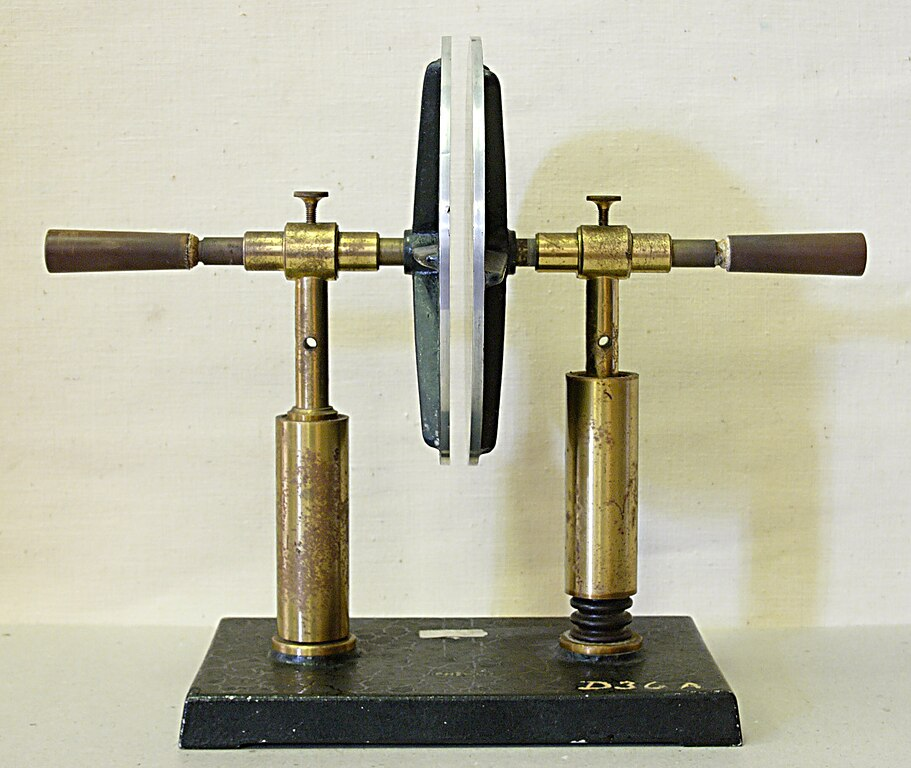
\includegraphics[height=0.25\textheight]{fig/lec03/Capacitor_example.jpg}
            
            {\small source: \href{https://commons.wikimedia.org/wiki/File:Plattenkondensator_hg.jpg}{Wikimedia Commons}, H.~Grobe, \href{https://creativecommons.org/licenses/by/3.0/deed.en}{CC~BY~3.0}}

            &

            \onslide<2->{
            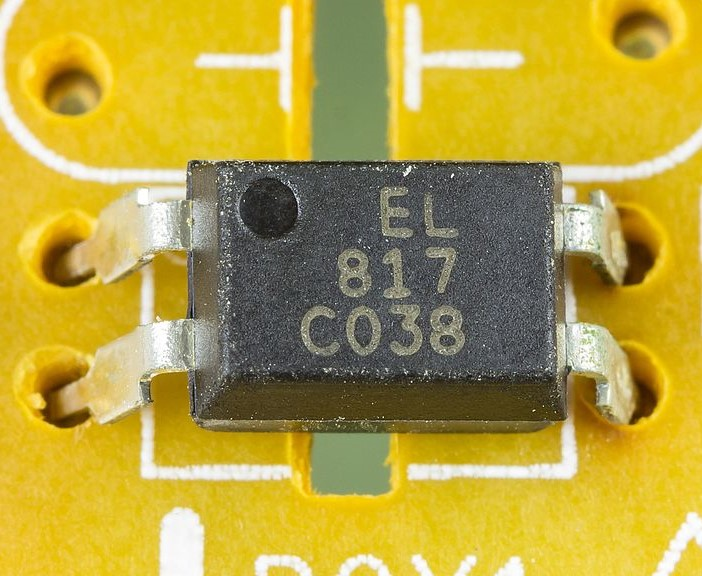
\includegraphics[height=0.25\textheight]{fig/lec03/Optocoupler_example.jpg}

            {\small source: \href{https://en.wikipedia.org/wiki/File:Philips_BDP3280-12_-_Everlight_EL817_on_power_board-1779.jpg}{Wikimedia Commons}, R.~Spekking, \href{https://creativecommons.org/licenses/by-sa/4.0/deed.en}{CC~BY-SA~4.0}}
            }

            &

            \onslide<3->{
            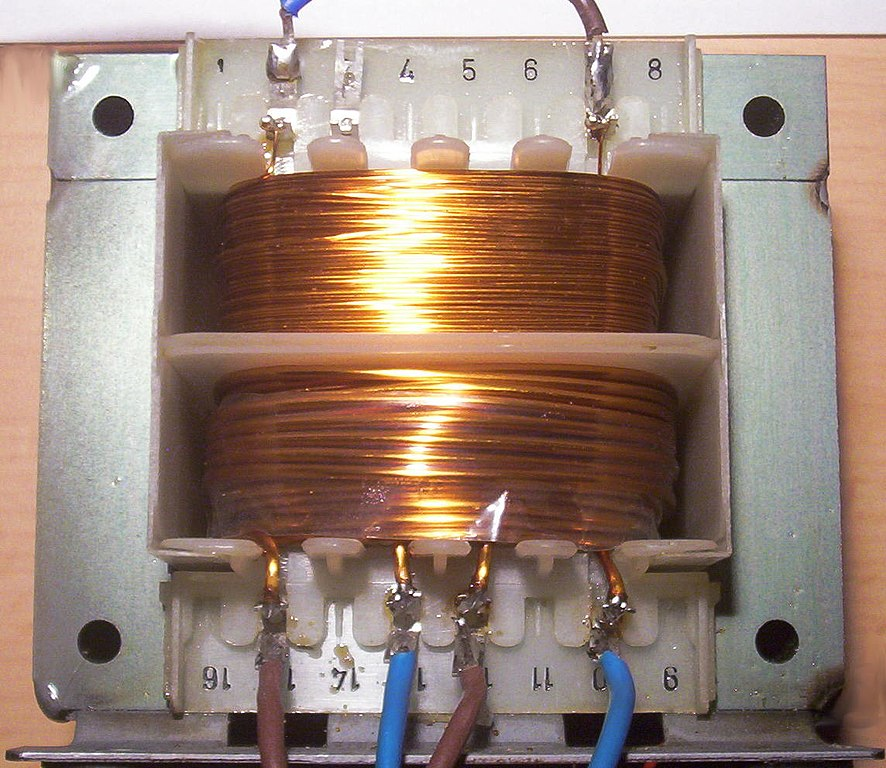
\includegraphics[height=0.25\textheight]{fig/lec03/Transformer_example.jpg}

            {\small source: \href{https://commons.wikimedia.org/wiki/File:Trafo-innenleben.jpg}{Wikimedia Commons}, S.~Riepl, public domain}
            }

		\end{tabular}
	\end{table}
\end{frame}

%%%%%%%%%%%%%%%%%%%%%%%%%%%%%%%%%%%%%%%%%%%%%%%%%%%%%%%%%%%%%
%% Galvanic isolation via transformer %%
%%%%%%%%%%%%%%%%%%%%%%%%%%%%%%%%%%%%%%%%%%%%%%%%%%%%%%%%%%%%%
\begin{frame}
    \frametitle{Galvanic isolation via transformer}
    \begin{columns}
        \begin{column}{0.4\textwidth}
            \begin{itemize}
                \item In power electronics, transformers are mostly used to provide galvanic isolation.
                \item<2-> Reason: the power density per volume and weight is typically higher than for capacitive or optical isolation.
                \item<3-> Assumptions for the following model:
                \begin{itemize}
                    \item<3-> Ideal coupling \newline(no leakage flux),
                    \item<4-> no losses,
                    \item<5-> no saturation.
                \end{itemize}
            \end{itemize}
        \end{column}
        \begin{column}{0.6\textwidth}
            \begin{figure}
                \begin{tikzpicture}[global scale/.style={scale=1.0}, rotate=-5, xslant=-0.1, thick, every
                    node/.style={transform shape, scale=0.8}, decoration={markings, mark=at position 0.5 with {\arrow{latex}}}]
                    \tikzmath{
                        real \a, \b, \dx, \dy, \lx, \ly, \dr;
                        \a = 3.0;
                        \b = 5.0;
                        \dx = 0.8;
                        \dy = 0.5;
                        \lx = 1.0;
                        \ly = 1.0;
                        \dr = 0.02;
                    } 
                    \begin{scope}[even odd rule, scale=0.9]
                    \filldraw[rounded corners=2pt, fill=gray, rotate=-0, opacity=1.0] (\dx,
                    \dy) rectangle ++(5,5) (\lx+\dx,\ly+\dy) rectangle ++(\a, \a);
                    \fill [rounded corners=2pt, fill=gray] (\b, 0) --++ (0, \dy+\dr+0.02) --++(\dx, 0) --cycle;
                    \fill [rounded corners=2pt, fill=gray] (0, \b) --++ (\dx+\dr+0.02, 0) --++(0, \dy)--cycle;
                    \filldraw[rounded corners=2pt, fill=gray!50, rotate=-0] (0,0) rectangle
                    ++(\b, \b) (\lx,\ly) rectangle ++(\a, \a);
                    \draw (\b-\dr,\dr) --++(\dx, \dy);
                    \draw (\b-\dr,\b-\dr) --++(\dx, \dy);
                    \draw (\dr,\b-\dr) --++(\dx, \dy);
                    \draw [signalalpha, thick, postaction={decorate}] (0, \ly) --++(-1.5,0);
                    \draw [rounded corners=2pt,signalalpha, thick]
                        (-0.09,\ly) -- (\lx, \ly)--++(0.89,0.5)
                        --++(-0.08, 0.05);
                    \foreach \z in {.24,.48,...,2.5}
                        {
                        \draw [rounded corners=2pt,signalalpha, thick]
                        (-0.0,\ly+\z+0.08)--(-0.09,\ly+\z) -- (\lx, \ly+\z)--++(0.89,0.5)
                        --++(-0.08, 0.05);
                    }
                    \draw [rounded corners=2pt,signalalpha, thick, postaction={decorate}] (-1.5,
                    \ly+2.8) --++(1.5,0) node[black, above, pos=0.4] {$i_1(t)$};
                    \draw[latex-] (-\lx, \ly+0.2) --++(0, 2.4) node[midway, left] {$u_1(t)$};
                    
                    \draw [rounded corners=2pt,signaldelta, thick] (\a+\lx-2*\dr,
                    \ly+2*\dr)--++(-\dr, -\dr)--++(\lx+\dx+2*\dr, 0);
                    \draw [signaldelta, postaction={decorate}] (\b+\dx-\dr+\a/2, \ly+\dr)--(\b+\dx-\dr, \ly+\dr);
                    \draw [rounded corners=2pt, signaldelta, thick, postaction={decorate}]
                    (\a+3*\lx-0.2, \ly+3.1) --++(\a/2, 0) node[black, midway, above] {$i_2(t)$};
                    \foreach \z in {.125,.25,.375,...,2.5}
                        {
                        \draw [rounded corners=2pt, signaldelta, thick] (\a+\lx,\ly+\z+0.1)--
                        (\a+\lx-0.07,\ly+\z) -- (\a+2*\lx, \ly+\z)--++(0.87,0.5)--++(-0.06,
                        0.06);
                        }
                    \draw[latex-] (2*\a+\lx, \ly+0.25) --++(0, 2.6) node[midway, left] {$u_2(t)$};
                    \end{scope}
                \end{tikzpicture}
                \caption{Simple transformer with primary and secondary winding}
                \label{fig:transformer_pseudo_3D}
            \end{figure}
        \end{column}
    \end{columns}
\end{frame}

%%%%%%%%%%%%%%%%%%%%%%%%%%%%%%%%%%%%%%%%%%%%%%%%%%%%%%%%%%%%%
%% Simplistic transformer model %%
%%%%%%%%%%%%%%%%%%%%%%%%%%%%%%%%%%%%%%%%%%%%%%%%%%%%%%%%%%%%%
\begin{frame}
    \frametitle{Simplistic transformer model}
    \begin{figure}
        \begin{subfigure}{0.4\textwidth}
            \centering
            \begin{tikzpicture}
                \draw (0,0) node[transformer core](T){$N_1:N_2$}
                (T.inner dot A1) node[circ]{}
                (T.inner dot B1) node[circ]{}
                (T.A1) to [short, -o, i<_=$i_1(t)$] ++(-1,0) coordinate (A1)
                (T.A2) to [short, -o] ++(-1,0) coordinate (A2)
                (T.B1) to [short, -o, i=$i_2(t)$] ++(1,0) coordinate (B1)
                (T.B2) to [short, -o] ++(1,0) coordinate (B2);
                \draw (A1) to [open, v=$u_1$, voltage = straight] (A2)
                (B1) to [open, v^=$u_2$, voltage = straight] (B2);
                \draw[dashed, thin] let \p1=(T.A1), \p2=(T.B2) in (\x1 + 2mm,\y1 + 10mm) rectangle (\x2 - 2mm,\y2 - 12.5mm)
                (\x1/2 + \x2/2,\y1 + 10mm) node[above] {Transformer};
            \end{tikzpicture}
           \caption{Schematic symbol representation} 
        \end{subfigure}
        \onslide<2->{%
            \begin{subfigure}{0.4\textwidth}
                \centering
                \begin{tikzpicture}
                    \draw (0,0) node[transformer core](T){$N_1:N_2$}
                    (T.inner dot A1) node[circ]{}
                    (T.inner dot B1) node[circ]{}
                    (T.A1) to [short, -*, i<_=$i'_1(t)$] ++(-1,0) coordinate (A1)
                    (T.A2) to [short, -*] ++(-1,0) coordinate (A2)
                    (A1) to [inductor, l=$L_\mathrm{m}$, i=$i_\mathrm{m}(t)$] (A2)
                    (A1) to [short, -o, i<_=$i_1(t)$] ++(-1.5,0) coordinate (A11)
                    (A2) to [short, -o] ++(-1.5,0) coordinate (A22)
                    (T.B1) to [short, -o, i=$i_2(t)$] ++(1,0) coordinate (B1)
                    (T.B2) to [short, -o] ++(1,0) coordinate (B2);
                    \draw (A11) to [open, v=$u_1$, voltage = straight] (A22)
                    (B1) to [open, v^=$u_2$, voltage = straight] (B2);
                    \draw[dashed, thin] let \p1=(A1), \p2=(T.B2) in (\x1 - 3mm,\y1 + 10mm) rectangle (\x2,\y2 - 12.5mm)
                    (\x1/2 + \x2/2 -2.5mm,\y1 + 10mm) node[above] {Transformer};
                    \draw[dashed, thin] let \p1=(T.A1), \p2=(T.B2) in (\x1 + 2mm,\y1 + 5mm) rectangle (\x2 - 2mm,\y2 - 2.5mm)
                    (\x1/2 + \x2/2,\y2 - 2.5mm) node[below, align=center] {Ideal\\ transformer};
                \end{tikzpicture}
                \caption{Equivalent circuit model} 
            \end{subfigure}
        }%
        \caption{Transformer model}
        \label{fig:transformer_model}
    \end{figure}
\end{frame}

%%%%%%%%%%%%%%%%%%%%%%%%%%%%%%%%%%%%%%%%%%%%%%%%%%%%%%%%%%%%%
%% Simplistic transformer model (cont.) %%
%%%%%%%%%%%%%%%%%%%%%%%%%%%%%%%%%%%%%%%%%%%%%%%%%%%%%%%%%%%%%
\begin{frame}
    \frametitle{Simplistic transformer model (cont.)}
    Based on \figref{fig:transformer_model} we consider the transformer as a combination of an ideal transformer with the \hl{conversion ratios}
    \begin{equation}
        \frac{u_1(t)}{u_2(t)} = \frac{N_1}{N_2} \quad \text{and} \quad \frac{i'_1(t)}{i_2(t)} = \frac{N_2}{N_1}
    \end{equation}\pause%
    and an inductor with the \hl{magnetizing inductance} $L_\mathrm{m}$:
    \begin{equation}
        u_1(t) = L_\mathrm{m} \frac{\mathrm{d}i_\mathrm{m}(t)}{\mathrm{d}t} \quad \text{and} \quad i_1(t) = i'_1(t) + i_\mathrm{m}(t).
    \end{equation}\pause %
    \begin{itemize}
        \item<3-> $L_\mathrm{m}$ models the magnetic energy stored in the transformer.
        \item<4-> Above model is a significant simplification (very first principle approach).
        \item<5-> More details on the transformer model can be found in the \href{https://github.com/IAS-Uni-Siegen/EMD_course}{Electrical Machines and Drives} course material.
    \end{itemize}
\end{frame}

%%%%%%%%%%%%%%%%%%%%%%%%%%%%%%%%%%%%%%%%%%%%%%%%%%%%%%%%%%%%%
%% Flyback converter %%
%%%%%%%%%%%%%%%%%%%%%%%%%%%%%%%%%%%%%%%%%%%%%%%%%%%%%%%%%%%%%
\subsection{Flyback converter}

%%%%%%%%%%%%%%%%%%%%%%%%%%%%%%%%%%%%%%%%%%%%%%%%%%%%%%%%%%%%%
%% Topology derivation based on the inverting buck-boost converter %%
%%%%%%%%%%%%%%%%%%%%%%%%%%%%%%%%%%%%%%%%%%%%%%%%%%%%%%%%%%%%%
\begin{frame}
    \frametitle{Topology derivation based on the inverting buck-boost converter}
    \begin{figure}
        \begin{circuitikz}[]
            \draw (0,0) to [short, *-] ++(1.0,0)
            to [diode, l=$D$, invert]  ++(1.0,0)
            to [short, -o, i=$i_2(t)$] ++(1.0,0)
            to [open, o-o, v^= $u_2(t)$, voltage = straight] ++(0,-2) coordinate (A)
            (0,0) to [short, *-] ++(-1.0,0) 
            to [Tnpn, n=npn1] ++(-1.0,0)
            to [short, -o, i_<=$i_1(t)$] ++(-1.0,0)
            to [open, o-o, v_= $u_1(t)$, voltage = straight] ++(0,-2)
            to [short, o-o] (A)
            (0,0) to [inductor, *-*] ++(0,-2);
            \draw let \p1 = (npn1.B) in node[anchor=north] at (\x1,\y1) {$T$};
            \draw [decorate,decoration={brace,amplitude=10pt,mirror,raise=0.5cm},yshift=0pt] (-3,-2.0) -- (3,-2.0) node [black,midway,yshift=-0.6cm] {};
        \end{circuitikz}
        \begin{circuitikz}[]
            \draw (0,0) to [short] ++(1.0,0)
            to [diode, l=$D$, invert]  ++(1.0,0)
            to [short, -o, i=$i_2(t)$] ++(1.0,0)
            to [open, o-o, v^= $u_2(t)$, voltage = straight] ++(0,-2) coordinate (A)
            (0,0) to [short] ++(-1.0,0) 
            to [Tnpn, n=npn1] ++(-1.0,0)
            to [short, -o, i_<=$i_1(t)$] ++(-1.0,0)
            to [open, o-o, v_= $u_1(t)$, voltage = straight] ++(0,-2)
            to [short, o-o] (A)
            (-0.5,0) to [inductor, *-*, n=l1] ++(0,-2)
            (0.5,0) to [inductor, *-*, n=l2, mirror] ++(0,-2);
            \draw let \p1 = (npn1.B) in node[anchor=north] at (\x1,\y1) {$T$};
            \path (l1.ul dot) node[circ]{}
                (l2.ul dot) node[circ]{};
            \draw (l1.midtap) node[left]{$N_1$}
            (l2.midtap) node[right]{$N_2$};
            \draw[double, double distance=3pt, thick] let \p1=(l1.core west), \p2=(l2.core east) in (\x1/2+\x2/2, \y1) -- (\x1/2+\x2/2, \y2);
        \end{circuitikz}
    \end{figure}
\end{frame}

%%%%%%%%%%%%%%%%%%%%%%%%%%%%%%%%%%%%%%%%%%%%%%%%%%%%%%%%%%%%%
%% Topology derivation based on the inverting buck-boost converter (cont.) %%
%%%%%%%%%%%%%%%%%%%%%%%%%%%%%%%%%%%%%%%%%%%%%%%%%%%%%%%%%%%%%
\begin{frame}
    \frametitle{Topology derivation based on the inverting buck-boost converter (cont.)}
    \begin{figure}
        \begin{circuitikz}[]
            \draw (0,0) to [short] ++(1.0,0)
            to [diode, l=$D$, invert]  ++(1.0,0)
            to [short, -o, i=$i_2(t)$] ++(1.0,0)
            to [open, o-o, v^= $u_2(t)$, voltage = straight] ++(0,-2) coordinate (A)
            (0,0) to [short] ++(-1.0,0) 
            to [Tnpn, n=npn1] ++(-1.0,0)
            to [short, -o, i_<=$i_1(t)$] ++(-1.0,0)
            to [open, o-o, v_= $u_1(t)$, voltage = straight] ++(0,-2)
            to [short, o-o] (A)
            (-0.5,0) to [inductor, *-*, n=l1] ++(0,-2)
            (0.5,0) to [inductor, *-*, n=l2, mirror] ++(0,-2);
            \draw let \p1 = (npn1.B) in node[anchor=north] at (\x1,\y1) {$T$};
            \path (l1.ul dot) node[circ]{}
                (l2.ul dot) node[circ]{};
            \draw (l1.midtap) node[left]{$N_1$}
            (l2.midtap) node[right]{$N_2$};
            \draw[double, double distance=3pt, thick] let \p1=(l1.core west), \p2=(l2.core east) in (\x1/2+\x2/2, \y1) -- (\x1/2+\x2/2, \y2);
            \draw [decorate,decoration={brace,amplitude=10pt,mirror,raise=0.5cm},yshift=0pt] (-3,-2.0) -- (3,-2.0) node [black,midway,yshift=-0.6cm] {};
        \end{circuitikz}
        \begin{circuitikz}[]
            \draw (0.5,0) to [short] ++(0.5,0)
            to [diode, l=$D$, invert]  ++(1.0,0)
            to [short, -o, i=$i_2(t)$] ++(1.0,0)
            to [open, o-o, v^= $u_2(t)$, voltage = straight] ++(0,-2) coordinate (A)
            (-0.5,0) to [short] ++(-0.5,0) 
            to [Tnpn, n=npn1] ++(-1.0,0)
            to [short, -o, i_<=$i_1(t)$] ++(-1.0,0)
            to [open, o-o, v_= $u_1(t)$, voltage = straight] ++(0,-2) coordinate (B)
            (-0.5,0) to [inductor, n=l1] ++(0,-2) coordinate (C)
            (0.5,0) to [inductor, n=l2, mirror] ++(0,-2) coordinate (D)
            (D) to [short, -o] (A)
            (C) to [short, -o] (B);
            \draw let \p1 = (npn1.B) in node[anchor=north] at (\x1,\y1) {$T$};
            \path (l1.ul dot) node[circ]{}
                (l2.ul dot) node[circ]{};
            \draw (l1.midtap) node[left]{$N_1$}
            (l2.midtap) node[right]{$N_2$};
            \draw[double, double distance=3pt, thick] let \p1=(l1.core west), \p2=(l2.core east) in (\x1/2+\x2/2, \y1) -- (\x1/2+\x2/2, \y2);
        \end{circuitikz}
    \end{figure}
\end{frame}

%%%%%%%%%%%%%%%%%%%%%%%%%%%%%%%%%%%%%%%%%%%%%%%%%%%%%%%%%%%%%
%% Flyback converter: topology %%
%%%%%%%%%%%%%%%%%%%%%%%%%%%%%%%%%%%%%%%%%%%%%%%%%%%%%%%%%%%%%
\begin{frame}
    \frametitle{Flyback converter: topology}
    \begin{columns}
        \begin{column}{0.5\textwidth}
            \begin{itemize}
                \item \hl{Flyback converter = non-inverting, galvanically isolated buck-boost converter}.
                \item<2-> Polarity change of primary and secondary transformer windings compensate for the inverting buck-boost characteristic.
                \item<3-> Transistor $T$ is placed below the transformer to enable a fixed emitter / source potential (beneficial for driver).
                \item<4-> Transformer's magnetizing inductance serves as the converter's energy buffer.
            \end{itemize}
        \end{column}
        %
        \begin{column}{0.5\textwidth}
            \begin{figure}
                \begin{circuitikz}[]
                    \draw (0.5,0) to [short] ++(0.5,0)
                    to [diode, l=$D$]  ++(1.0,0)
                    to [short, -o, i=$i_2(t)$] ++(1.0,0)
                    to [open, o-o, v^= $u_2(t)$, voltage = straight] ++(0,-2) coordinate (A)
                    (-0.5,0) to [short, -o, i_<=$i_1(t)$] ++(-1.5,0)
                    to [open, o-o, v_= $u_1(t)$, voltage = straight] ++(0,-3.75) coordinate (B)
                    (-0.5,0) to [inductor, n=l1] ++(0,-2) 
                    to [Tnpn, n=npn1, invert] ++(0,-1.75) coordinate (C)
                    (0.5,0) to [inductor, n=l2, mirror] ++(0,-2) coordinate (D)
                    (D) to [short, -o] (A)
                    (C) to [short, -o] (B);
                    \draw let \p1 = (npn1.B) in node[anchor=south] at (\x1,\y1) {$T$};
                    \path (l1.ul dot) node[circ]{}
                        (l2.ur dot) node[circ]{};
                    \draw (l1.midtap) node[left]{$N_1$}
                    (l2.midtap) node[right]{$N_2$};
                    \draw[double, double distance=3pt, thick] let \p1=(l1.core west), \p2=(l2.core east) in (\x1/2+\x2/2, \y1) -- (\x1/2+\x2/2, \y2);
                \end{circuitikz}
                \caption{Flyback converter topology}
                \label{fig:flyback_converter_topology}
            \end{figure}
        \end{column}
    \end{columns}
\end{frame}

%%%%%%%%%%%%%%%%%%%%%%%%%%%%%%%%%%%%%%%%%%%%%%%%%%%%%%%%%%%%%
%% Flyback converter: switching states %%
%%%%%%%%%%%%%%%%%%%%%%%%%%%%%%%%%%%%%%%%%%%%%%%%%%%%%%%%%%%%%
\begin{frame}
    \frametitle{Flyback converter: switching states in CCM}
    \begin{itemize}
        \item Switch-on time: rising primary current induces a negative voltage at the transformer's secondary winding leading to blocking diode. Energy is stored in $L_\mathrm{m}$.
        \item<2-> Switch-off time: primary current is blocked by transistor and an equivalent current is induced in the secondary winding. Energy is taken from $L_\mathrm{m}$.
    \end{itemize}
    \begin{figure}
        \begin{subfigure}{0.45\textwidth}
            \centering
            \begin{circuitikz}[]
                \draw (0.5,0) to [short] ++(0.5,0)
                to [open]  ++(1.0,0)
                to [short, -o, i={$i_2(t)=0$}] ++(1.0,0)
                to [open, o-o, v^= $u_2(t)$, voltage = straight] ++(0,-2) coordinate (A)
                (-0.5,0) to ++(-1,0) coordinate (E)
                to [short, -o, i_<=$i_1(t)$] ++(-1.0,0)
                to [open, o-o, v_= $u_1(t)$, voltage = straight] ++(0,-3) coordinate (B)
                (-0.5,0) to [inductor, n=l1] ++(0,-2) 
                to [short] ++(0,-1) coordinate (C)
                (0.5,0) to [inductor, n=l2, mirror] ++(0,-2) coordinate (D)
                (D) to [short, -o] (A)
                (C) to [short, -o] (B)
                (E) to [inductor, l_=$L_\mathrm{m}$, i=$i_\mathrm{m}(t)$, *-] ++(0,-2) 
                to [short, -*] ++(1.0,0);
                \path (l1.ul dot) node[circ]{}
                    (l2.ur dot) node[circ]{};
                \draw (l1.midtap) node[left]{$N_1$}
                (l2.midtap) node[right]{$N_2$};
                \draw[double, double distance=3pt, thick] let \p1=(l1.core west), \p2=(l2.core east) in (\x1/2+\x2/2, \y1) -- (\x1/2+\x2/2, \y2);
            \end{circuitikz}
            \caption{Switch-on time}
        \end{subfigure}
        \hspace{0.75cm}
        \onslide<2->{%
            \begin{subfigure}{0.45\textwidth}
                \centering
                \begin{circuitikz}[]
                    \draw (0.5,0) to [short] ++(0.5,0)
                    to [short, -o, i={$i_2(t)$}] ++(0.75,0)
                    to [open, o-o, v^= $u_2(t)$, voltage = straight] ++(0,-2) coordinate (A)
                    (-0.5,0) to ++(-1,0) coordinate (E)
                    to [short, -o, i_<={$i_1(t)=0$}] ++(-1.0,0)
                    to [open, o-o, v_= $u_1(t)$, voltage = straight] ++(0,-3) coordinate (B)
                    (-0.5,0) to [inductor, n=l1] ++(0,-2) 
                    to [open] ++(0,-1) coordinate (C)
                    (0.5,0) to [inductor, n=l2, mirror] ++(0,-2) coordinate (D)
                    (D) to [short, -o] (A)
                    (C) to [short, -o] (B)
                    (E) to [inductor, l_=$L_\mathrm{m}$, i=$i_\mathrm{m}(t)$, *-] ++(0,-2) 
                    to [short] ++(1.0,0);;
                    \path (l1.ul dot) node[circ]{}
                        (l2.ur dot) node[circ]{};
                    \draw (l1.midtap) node[left]{$N_1$}
                    (l2.midtap) node[right]{$N_2$};
                    \draw[double, double distance=3pt, thick] let \p1=(l1.core west), \p2=(l2.core east) in (\x1/2+\x2/2, \y1) -- (\x1/2+\x2/2, \y2);
                \end{circuitikz}
                \caption{Switch-off time}            
            \end{subfigure}
        }%
            \centering
        \caption{Switch states of the flyback converter}
        \label{fig:flyback-converter-switch-states}
    \end{figure}
\end{frame}

%%%%%%%%%%%%%%%%%%%%%%%%%%%%%%%%%%%%%%%%%%%%%%%%%%%%%%%%%%%%%
%% Flyback converter: steady-state time-domain behavior in CCM %%
%%%%%%%%%%%%%%%%%%%%%%%%%%%%%%%%%%%%%%%%%%%%%%%%%%%%%%%%%%%%%
\begin{frame}[fragile]
    \frametitle{Flyback converter: steady-state time-domain behavior in CCM}
    \begin{figure}
        \begin{tikzpicture}
            \pgfmathsetmacro{\D}{0.4} % duty cycle
            \pgfmathsetmacro{\n}{0.7} % turns ration n= N2/N1
            \pgfmathsetmacro{\gain}{\n*\D/(1-\D)} % current ripple
            \begin{groupplot}[group style={group size=1 by 3, xticklabels at = edge bottom}, height=0.34\textheight, width=0.875\textwidth, xmin=0, xmax=4, grid,clip = false, ymin = 0, ymax =1.1]

                % Top plot: voltage at the switch
                \nextgroupplot[ylabel = {$u_\mathrm{L_\mathrm{m}}(t)$}, ytick = {-1, -0.5, 0, 0.5, 1}, yticklabels = {$-U_1$, , 0, , $U_1$}, ymin = -1.1, ymax = 1.1]
                    \pgfplotsinvokeforeach{0,...,3}{
                        \edef\AddPlot{\noexpand\addplot[signalalpha, thick] coordinates {({0 + #1},-\gain) ({0 + #1},1) ({\D + #1},1) ({\D + #1},-\gain) ({1 + #1},-\gain) ({1 + #1},1)};}
                        \AddPlot
                    }
                    \node[above, inner sep = 2pt, anchor = south] at (axis cs:1.5+\D/2, -\gain) {$-U_2\frac{N_1}{N_2}$}; % label U_2
                    \draw [thick,<->]  (0,0.6) -- node[below]{$T_\mathrm{on}$}(\D, 0.6); % T_on 
                    \draw [thick,<->]  (\D,0.6) -- node[below]{$T_\mathrm{off}$}(1.0, 0.6); % T_off
                    \draw [thick,<->]  (0.0,-1.4) -- node[below]{$T_\mathrm{s}$}(1.0, -1.4); % T_s 


                % Middle plot: inductor current
                \nextgroupplot[ylabel = {$i_\mathrm{m}(t)$}, ytick = {0, 0.5, 1}, yticklabels = {0, $\overline{i}_\mathrm{m}$, }]
                    \pgfplotsinvokeforeach{0,...,3}{
                        \edef\AddPlot{\noexpand\addplot[signaldelta, thick] coordinates {({0 + #1},0.25) ({\D + #1},0.75) ({1 + #1},0.25)};}
                        \AddPlot
                    }
                    \draw[signaldelta, thick, dashed] (axis cs:0,0.5) -- (axis cs:4,0.5); % dashed line at average current
                    \draw[{Latex[length=2mm]}-, thin] (axis cs:\D+0.02,0.75) -- node[right=1mm, fill=white, inner sep = 1pt]{$\max\{i_\mathrm{m}\}$}(axis cs:\D+0.3,0.9); % indicate max current
                    \draw[-{Latex[length=2mm]}, thin] (axis cs:0.75,0.2) node[right=1mm, fill=white, inner sep = 1pt, anchor = east]{$\min\{i_\mathrm{m}\}$} -- (axis cs:1-0.02,0.25); % indicate min current
                    \draw[thin] (axis cs:2+\D/4,0.25+0.125) -- (axis cs:2+\D/4,0.75-0.125) -- (axis cs:2+\D*3/4,0.75-0.125); % indicate positive current slopde
                    \node[above, inner sep = 2pt, anchor = south, xshift = -4mm] at (axis cs:2+\D/2, 0.75-0.125) {$\nicefrac{U_1}{L_\mathrm{m}}$}; % label positive current slope
                    \draw[thin] (axis cs:2.25+3*\D/4,0.75-0.125) -- (axis cs:2.75+\D/4,0.75-0.125) -- (axis cs:2.75+\D/4,0.25+0.125); % indicate negative current slope
                    \node[above, inner sep = 2pt, anchor = south, xshift = 2mm] at (axis cs:2.5+\D/2, 0.75-0.125) {$\nicefrac{-U_2\frac{N_1}{N_2}}{L_\mathrm{m}}$}; % label negative current slope
                
                % Bottom plot: input current
                \nextgroupplot[ylabel = {$i_1(t)$}, xlabel={$t/T_\mathrm{s}$}, ytick = {0, 0.5, 1}, yticklabels = {0, ,}]
                    \pgfplotsinvokeforeach{0,...,3}{
                        \edef\AddPlot{\noexpand\addplot[signaldelta, thick] coordinates {({0 + #1},0.25) ({\D + #1},0.75) ({\D + #1},0) ({1 + #1},0) ({1 + #1},0.25)};}
                        \AddPlot
                    }
                    \draw[signaldelta, thick, dashed] (axis cs:0,0.5 * \D) -- (axis cs:4, 0.5 * \D); % dashed line at average current
                    \node[signaldelta, above, inner sep = 1pt, anchor = east, fill = white, xshift=-1mm] at (axis cs:\D, 0.5 * \D) {$\overline{i}_1$}; % label average current
                    \node[signaldelta, above, inner sep = 2pt, anchor = center, fill = white] at (axis cs:\D/2-0.05, 0.85) {$i_1(t)$}; % label input current
            \end{groupplot}

            % second y-axis for the bottom plot
					\begin{groupplot}[group style={group size=1 by 3, y descriptions at = edge right}, height=0.34\textheight, width=0.875\textwidth, xmin=0, xmax=4, grid,clip = false, xtick=\empty, axis line style=transparent, ymin = 0, ymax =1.1]
						\nextgroupplot[ytick = \empty]
							%
                        \nextgroupplot[ytick = \empty, ymin =-1.1]
                        %
						\nextgroupplot[ylabel = {$i_2(t)$}, ytick = {}, yticklabels = {}]
                            \pgfplotsinvokeforeach{0,...,3}{
                                \edef\AddPlot{\noexpand\addplot[signalalpha, thick] coordinates {({0 + #1},0) ({\D + #1},0) ({\D + #1},0.75/\n) ({1 + #1},0.25/\n) ({1 + #1},0)};}
                                \AddPlot
                            }
                            \node[signalalpha, above, inner sep = 2pt, anchor = center, fill = white] at (axis cs:0.95, 0.85) {$i_2(t)$}; % label output current
                            \draw[signalalpha, thick, dashed] (axis cs:0,0.5/\n-0.5*\D/\n) -- (axis cs:4, 0.5/\n-0.5*\D/\n); % dashed line at average current
                            \node[signalalpha, above, inner sep = 1pt, anchor = west, fill = white, xshift=1mm] at (axis cs:\D, 0.5/\n-0.5*\D/\n) {$\overline{i}_2$}; % label average current
					\end{groupplot}
        \end{tikzpicture}
    \end{figure}
\end{frame}

%%%%%%%%%%%%%%%%%%%%%%%%%%%%%%%%%%%%%%%%%%%%%%%%%%%%%%%%%%%%%
%% Flyback converter: impact of the transformer turns ratio %%
%%%%%%%%%%%%%%%%%%%%%%%%%%%%%%%%%%%%%%%%%%%%%%%%%%%%%%%%%%%%%
\begin{frame}
    \frametitle{Flyback converter: impact of the transformer turns ratio}
    \begin{columns}
        \begin{column}{0.5\textwidth}
           The transformer scales the peak input and output current according to the turns ratio $\nicefrac{N_2}{N_1}$ (with $\varepsilon$ being a small time period)
            \begin{equation*}
                i_2(t=T_\mathrm{on}+\varepsilon) = \frac{N_1}{N_2} i_1(t=T_\mathrm{on}-\varepsilon),
            \end{equation*}
            i.e., the output side may carry significantly different peak currents than the input.
            \onslide<2->{
            Also, when the transistor blocks it must withstand the voltage
            \begin{equation*}
                u_\mathrm{T}(t) = u_1 (t) + \frac{N_1}{N_2}u_2 (t), \quad t\in [T_\mathrm{on}, T_\mathrm{s}].
            \end{equation*}
            Hence, the turn ratio has a significant impact on components' stress factors.
            }%
        \end{column}
        %
        \begin{column}{0.5\textwidth}
            \begin{figure}
                \begin{tikzpicture}
                    \pgfmathsetmacro{\D}{0.6} % duty cycle
                    \pgfmathsetmacro{\n}{0.6} % turns ration n= N2/N1
                    \pgfmathsetmacro{\ioff}{0.2} % offset current / min current primary side
                    \begin{axis}[
                        xlabel={$t$},
                        ymin=0, ymax=1/\n+0.1,
                        xmin=-\D-0.1, xmax=(1-\D)+0.1,
                        width = \textwidth,
                        height = 0.7\textheight,
                        grid,
                        thick,
                        clip = true,
                        axis lines=middle,
                        ytick = {0, 1, 1/\n}, 
                        yticklabels = {0, $\max\{i_1\}$, $\frac{N_1}{N_2}\max\{i_1\}$},
                        xtick = {-\D, 0.001, 1-\D},
                        xticklabels = {$0$, $T_\mathrm{on}$, $T_\mathrm{s}$},
                        ]
                        \addplot[signaldelta] coordinates {(-\D,0) (-\D,\ioff) (0,1) (0,0) (1-\D, 0)};
                        \addplot[signalalpha] coordinates {(-\D,0)  (0,0) (0,1/\n) (1-\D, \ioff/\n) (1-\D, 0)};
                        \addplot[signalalpha, dashed] coordinates {(-1,1/\n) (-\D,\ioff/\n) (-\D,0)};
                        \addplot[signaldelta, dashed] coordinates {(1-\D, 0) (1-\D, \ioff) (1, 1)};
                        \node[signalalpha, above, inner sep = 2pt, anchor = south, fill = white] at (axis cs:\D/2, 1) {$i_2(t)$};
                        \node[signaldelta, above, inner sep = 2pt, anchor = center, fill = white] at (axis cs:-\D/2, 0.3) {$i_1(t)$};
                    \end{axis}
                \end{tikzpicture}
                \caption{Example of the ratio of the input and output current for $\nicefrac{N_2}{N_1}=0.6$}
            \end{figure}
        \end{column}
    \end{columns}
\end{frame}

%%%%%%%%%%%%%%%%%%%%%%%%%%%%%%%%%%%%%%%%%%%%%%%%%%%%%%%%%%%%%
%% Flyback converter: voltage voltage transfer ratio in CCM %%
%%%%%%%%%%%%%%%%%%%%%%%%%%%%%%%%%%%%%%%%%%%%%%%%%%%%%%%%%%%%%

\begin{frame}
    \frametitle{Flyback converter: voltage transfer ratio in CCM}
    \onslide<1->{
    In CCM, the voltage balance of the magnetizing inductor $L_\mathrm{m}$ delivers:
    \begin{equation}
        u_\mathrm{L_\mathrm{m}}(t) = \begin{cases} 
            U_1, & t\in [k T_\mathrm{s}, k T_\mathrm{s} + T_\mathrm{on}],\\ 
            -\frac{N_1}{N_2}U_2 & t\in [k T_\mathrm{s} + T_\mathrm{on}, (k+1) T_\mathrm{s}].
        \end{cases}
    \end{equation}}%
    \onslide<2->{In steady state, the average inductor voltage per period must be zero, yielding}%
    \begin{equation}
        \onslide<2->{U_1 T_\mathrm{on} = \frac{N_1}{N_2} U_2 T_\mathrm{off}  \quad}\onslide<3->{ \Leftrightarrow \quad  U_1 D T_\mathrm{s} = \frac{N_1}{N_2}U_2 (1-D) T_\mathrm{s} \quad}\onslide<4->{ \Leftrightarrow \quad \frac{U_2}{U_1} = \frac{N_2}{N_1}\frac{D}{1-D}.}
    \end{equation}
    \begin{itemize}
        \item<5-> Structurally similar result to the (inverting/synchronous) buck-boost converter.
        \item<6-> The voltage transfer ratio is additionally scaled by the turns ratio $\nicefrac{N_2}{N_1}$.
        \item<7-> The flyback's tranformer enables additional degrees of freedom to achieve a certain voltage transfer ratio via $D$ and $\nicefrac{N_2}{N_1}$.
    \end{itemize}
\end{frame}

%%%%%%%%%%%%%%%%%%%%%%%%%%%%%%%%%%%%%%%%%%%%%%%%%%%%%%%%%%%%%
%% Flyback converter: switch states %%
%%%%%%%%%%%%%%%%%%%%%%%%%%%%%%%%%%%%%%%%%%%%%%%%%%%%%%%%%%%%%

\begin{frame}
    \frametitle{Flyback converter: switch states in DCM}
    \onslide<1->{The flyback converter in DCM has three different switch states:}
    \begin{itemize}
            \item<1-> Transistor on-time:  $T_\mathrm{on}=DT_\mathrm{s}$,
            \item<2-> Transistor off-time (conducting diode): $T'_\mathrm{off}=D'T_\mathrm{s}$,
            \item<3-> Transistor off-time (no conduction):  $T''_\mathrm{off}=T_\mathrm{s}-T_\mathrm{on}-T'_\mathrm{off}$.
    \end{itemize}
    \begin{figure}
        \centering
        \onslide<1->{%	
        \begin{subfigure}{0.33\textwidth}
            \centering
            \begin{circuitikz}[scale=0.8, transform shape]
                \draw (0.5,0) to [short] ++(0.5,0)
                to [open]  ++(1.0,0)
                to [short, -o, i={$i_2=0$}] ++(0.75,0)
                to [open, o-o, v= $u_2$, voltage = straight] ++(0,-2) coordinate (A)
                (-0.5,0) to ++(-1,0) coordinate (E)
                to [short, -o, i_<=$i_1$] ++(-1.0,0)
                to [open, o-o, v^=$u_1$, voltage = straight] ++(0,-3) coordinate (B)
                (-0.5,0) to [inductor, n=l1] ++(0,-2) 
                to [short] ++(0,-1) coordinate (C)
                (0.5,0) to [inductor, n=l2, mirror] ++(0,-2) coordinate (D)
                (D) to [short, -o] (A)
                (C) to [short, -o] (B)
                (E) to [inductor, l_=$L_\mathrm{m}$, i=$i_\mathrm{m}$, *-] ++(0,-2) 
                to [short, -*] ++(1.0,0);
                \path (l1.ul dot) node[circ]{}
                    (l2.ur dot) node[circ]{};
                \draw (l1.midtap) node[left]{$N_1$}
                (l2.midtap) node[right]{$N_2$};
                \draw[double, double distance=3pt, thick] let \p1=(l1.core west), \p2=(l2.core east) in (\x1/2+\x2/2, \y1) -- (\x1/2+\x2/2, \y2);
            \end{circuitikz}
            \caption{Switch-on time $T_\mathrm{on}$}
        \end{subfigure}%
        }%
        \onslide<2->{%
        \begin{subfigure}{0.33\textwidth}
            \centering
            \hspace{-0.6cm}
            \begin{circuitikz}[scale=0.8, transform shape]
                \draw (0.5,0) to [short] ++(0.5,0)
                to [short, -o, i={$i_2$}] ++(0.75,0)
                to [open, o-o, v = $u_2$, voltage = straight] ++(0,-2) coordinate (A)
                (-0.5,0) to ++(-1,0) coordinate (E)
                to [short, -o, i_<={$i_1=0$}] ++(-1.0,0)
                to [open, o-o, v^= $u_1$, voltage = straight] ++(0,-3) coordinate (B)
                (-0.5,0) to [inductor, n=l1] ++(0,-2) 
                to [open] ++(0,-1) coordinate (C)
                (0.5,0) to [inductor, n=l2, mirror] ++(0,-2) coordinate (D)
                (D) to [short, -o] (A)
                (C) to [short, -o] (B)
                (E) to [inductor, l_=$L_\mathrm{m}$, i=$i_\mathrm{m}$, *-] ++(0,-2) 
                to [short] ++(1.0,0);;
                \path (l1.ul dot) node[circ]{}
                    (l2.ur dot) node[circ]{};
                \draw (l1.midtap) node[left]{$N_1$}
                (l2.midtap) node[right]{$N_2$};
                \draw[double, double distance=3pt, thick] let \p1=(l1.core west), \p2=(l2.core east) in (\x1/2+\x2/2, \y1) -- (\x1/2+\x2/2, \y2);
            \end{circuitikz}
            \caption{Switch-off time $T'_\mathrm{off}$}
        \end{subfigure}
        }%
        \onslide<3->{%
        \begin{subfigure}{0.33\textwidth}
            \centering
            \begin{circuitikz}[scale=0.8, transform shape]
                \draw (0.5,0) to [short] ++(0.5,0)
                to [open]  ++(1.0,0)
                to [short, -o, i={$i_2=0$}] ++(0.75,0)
                to [open, o-o, v= $u_2$, voltage = straight] ++(0,-2) coordinate (A)
                (-0.5,0) to ++(-1,0) coordinate (E)
                to [short, -o, i_<={$i_1=0$}] ++(-1.0,0)
                to [open, o-o, v^=$u_1$, voltage = straight] ++(0,-3) coordinate (B)
                (-0.5,0) to [inductor, n=l1] ++(0,-2) 
                to [open] ++(0,-1) coordinate (C)
                (0.5,0) to [inductor, n=l2, mirror] ++(0,-2) coordinate (D)
                (D) to [short, -o] (A)
                (C) to [short, -o] (B)
                (E) to [inductor, l_=$L_\mathrm{m}$, i=$i_\mathrm{m}$, *-] ++(0,-2) 
                to [short, -] ++(1.0,0);
                \path (l1.ul dot) node[circ]{}
                    (l2.ur dot) node[circ]{};
                \draw (l1.midtap) node[left]{$N_1$}
                (l2.midtap) node[right]{$N_2$};
                \draw[double, double distance=3pt, thick] let \p1=(l1.core west), \p2=(l2.core east) in (\x1/2+\x2/2, \y1) -- (\x1/2+\x2/2, \y2);
            \end{circuitikz}
            \caption{Switch-off time $T''_\mathrm{off}$}
        \end{subfigure}
        }%
    \caption{Switch states of the flyback converter including DCM} 
    \label{fig:flyback-switch-states-DCM}
    \end{figure}
\end{frame}

%%%%%%%%%%%%%%%%%%%%%%%%%%%%%%%%%%%%%%%%%%%%%%%%%%%%%%%%%%%%%
%% Flyback converter: steady-state time-domain behavior in DCM %%
%%%%%%%%%%%%%%%%%%%%%%%%%%%%%%%%%%%%%%%%%%%%%%%%%%%%%%%%%%%%%
\begin{frame}[fragile]
    \frametitle{Flyback converter: steady-state time-domain behavior in DCM}
    \begin{figure}
        \begin{tikzpicture}
            \pgfmathsetmacro{\D}{0.4} % duty cycle
            \pgfmathsetmacro{\Doff}{0.3} % relative off time (diode conducting)
            \pgfmathsetmacro{\n}{0.7} % turns ration n= N2/N1
            \pgfmathsetmacro{\gain}{\n*\D/(1-\D)} % current ripple
            \begin{groupplot}[group style={group size=1 by 3, xticklabels at = edge bottom}, height=0.34\textheight, width=0.875\textwidth, xmin=0, xmax=4, grid,clip = false, ymin = 0, ymax =1.1]

                % Top plot: voltage at the switch
                \nextgroupplot[ylabel = {$u_\mathrm{L_\mathrm{m}}(t)$}, ytick = {-1, -0.5, 0, 0.5, 1}, yticklabels = {$-U_1$, , 0, , $U_1$}, ymin = -1.1, ymax = 1.1]
                    \pgfplotsinvokeforeach{0,...,3}{
                        \edef\AddPlot{\noexpand\addplot[signalalpha, thick] coordinates {({0 + #1},0) ({0 + #1},1) ({\D + #1},1) ({\D + #1},-\gain) ({\D + \Doff + #1},-\gain) ({\D + \Doff + #1}, 0) ({1 + #1},0) ({1 + #1},1)};}
                        \AddPlot
                    }
                    \node[above, inner sep = 2pt, anchor = west] at (axis cs:0.85, -\gain) {$-U_2\frac{N_1}{N_2}$}; % label U_2
                    \draw [thick,<->]  (0,-1.4) -- node[below]{$T_\mathrm{on}$}(\D, -1.4); % T_on 
                    \draw [thick,<->]  (\D,-1.4) -- node[below]{$T'_\mathrm{off}$}(\D+\Doff, -1.4); % T'_off
                    \draw [thick,<->]  (\D+\Doff,-1.4) -- node[below]{$T''_\mathrm{off}$}(1, -1.4); % T''_off
                    \draw [thick,<->]  (1.0,-1.4) -- node[below]{$T_\mathrm{s}$}(2.0, -1.4); % T_s 


                % Middle plot: inductor current
                \nextgroupplot[ylabel = {$i_\mathrm{m}(t)$}, ytick = {0, 0.5, 1}, yticklabels = {0, , }]
                    \pgfplotsinvokeforeach{0,...,3}{
                        \edef\AddPlot{\noexpand\addplot[signaldelta, thick] coordinates {({0 + #1},0) ({\D + #1},0.75) ({\D + \Doff + #1},0) ({1 + #1},0)};}
                        \AddPlot
                    }
                    \draw[signaldelta, thick, dashed] (axis cs:0,0.75/2*\D+0.75/2*\Doff) -- (axis cs:4,0.75/2*\D+0.75/2*\Doff); % dashed line at average current
                    \draw[{Latex[length=2mm]}-, thin] (axis cs:\D+0.02,0.75) -- node[right=1mm, fill=white, inner sep = 1pt]{$\max\{i_\mathrm{m}\}$}(axis cs:\D+0.3,0.9); % indicate max current
                    \draw[thin] (axis cs:2+\D/4,0.75/4) -- (axis cs:2+\D/4,0.75/4*3) -- (axis cs:2+\D*3/4,0.75/4*3); % indicate positive current slopde
                    \node[above, inner sep = 2pt, anchor = south, xshift = -4mm] at (axis cs:2+\D/2, 0.75-0.165) {$\nicefrac{U_1}{L_\mathrm{m}}$}; % label positive current slope
                    \draw[thin] (axis cs:2+\D+\Doff/4,0.75*3/4) -- (axis cs:2+\D+\Doff*3/4,0.75*3/4) -- (axis cs:2+\D+\Doff*3/4,0.75/4); % indicate negative current slope
                    \node[above, inner sep = 2pt, anchor = south, xshift = 2mm] at (axis cs:2.5+\D/2, 0.75-0.175) {$\nicefrac{-U_2\frac{N_1}{N_2}}{L_\mathrm{m}}$}; % label negative current slope
                
                % Bottom plot: input current
                \nextgroupplot[ylabel = {$i_1(t)$}, xlabel={$t/T_\mathrm{s}$}, ytick = {0, 0.5, 1}, yticklabels = {0, ,}]
                    \pgfplotsinvokeforeach{0,...,3}{
                        \edef\AddPlot{\noexpand\addplot[signaldelta, thick] coordinates {({0 + #1},0) ({\D + #1},0.75) ({\D + #1},0) ({1 + #1},0) ({1 + #1},0)};}
                        \AddPlot
                    }
                    \draw[signaldelta, thick, dashed] (axis cs:0,0.75/2 * \D) -- (axis cs:4, 0.75/2 * \D); % dashed line at average current
                    \node[signaldelta, above, inner sep = 1pt, anchor = south, fill = white] at (axis cs:3-\Doff/2, 0.75/2 * \D) {$\overline{i}_1$}; % label average current
                    \node[signaldelta, above, inner sep = 2pt, anchor = center, fill = white] at (axis cs:\D/2-0.05, 0.8) {$i_1(t)$}; % label input current
            \end{groupplot}

            % second y-axis for the bottom plot
					\begin{groupplot}[group style={group size=1 by 3, y descriptions at = edge right}, height=0.34\textheight, width=0.875\textwidth, xmin=0, xmax=4, grid,clip = false, xtick=\empty, axis line style=transparent, ymin = 0, ymax =1.1]
						\nextgroupplot[ytick = \empty]
							%
                        \nextgroupplot[ytick = \empty, ymin =-1.1]
                        %
						\nextgroupplot[ylabel = {$i_2(t)$}, ytick = {}, yticklabels = {}]
                            \pgfplotsinvokeforeach{0,...,3}{
                                \edef\AddPlot{\noexpand\addplot[signalalpha, thick] coordinates {({0 + #1},0) ({\D + #1},0) ({\D + #1},0.75/\n) ({\D + \Doff + #1},0) ({1 + #1},0)};}
                                \AddPlot
                            }
                            \node[signalalpha, above, inner sep = 2pt, anchor = center, fill = white] at (axis cs:0.75, 0.75) {$i_2(t)$}; % label output current
                            \draw[signalalpha, thick, dashed] (axis cs:0,0.75/2*\Doff/\n) -- (axis cs:4, 0.75/2*\Doff/\n); % dashed line at average current
                            \node[signalalpha, above, inner sep = 1pt, anchor = south, fill = white] at (axis cs:2-\Doff/2, 0.75/2*\Doff/\n) {$\overline{i}_2$}; % label average current
					\end{groupplot}
        \end{tikzpicture}
    \end{figure}
\end{frame}

%%%%%%%%%%%%%%%%%%%%%%%%%%%%%%%%%%%%%%%%%%%%%%%%%%%%%%%%%%%%%
%% Flyback converter: DCM operation characteristics %%
%%%%%%%%%%%%%%%%%%%%%%%%%%%%%%%%%%%%%%%%%%%%%%%%%%%%%%%%%%%%%
\begin{frame}
    \frametitle{Flyback converter: DCM operation characteristics}
    \onslide<1->{In DCM operation 
    $$  \overline{i}_\mathrm{m} < \frac{\Delta i_\mathrm{\mathrm{m}}}{2} \quad \Rightarrow \quad U_2 \neq U_1 \frac{N_2}{N_1}\frac{D}{1-D}$$
    applies due to the non-conducting diode during  $T''_\mathrm{off}$.} \onslide<2->{To find the input-to-output voltage ratio in DCM, we again utilize the current ripple balance:}
    \begin{equation}
        \begin{alignedat}{2}
            \onslide<2->{\Delta i_\mathrm{m} &= \frac{U_1}{L_\mathrm{m}}T_\mathrm{on} = \frac{U_1}{L_\mathrm{m}}DT_\mathrm{s} \quad &&\mbox{(rising edge)},}\\
            \onslide<3->{\Delta i_\mathrm{\mathrm{m}} &= \frac{N_1}{N_2}\frac{U_2}{L_\mathrm{m}}T'_\mathrm{off} = \frac{N_1}{N_2}\frac{U_2}{L_\mathrm{m}}D'T_\mathrm{s} \quad &&\mbox{(falling edge)}.}
        \end{alignedat}
    \end{equation}
    \onslide<4->{Solving for $D'$ yields
    \begin{equation}
        D' = \frac{N_2}{N_1}\frac{U_1}{U_2}D.
    \end{equation}}
    \onslide<5->{The average load current is }
    \begin{equation}
        \onslide<5->{\overline{i}_2 = \frac{N_1}{N_2}\frac{\Delta i_\mathrm{m}}{2}\frac{T'_\mathrm{off}}{T_\mathrm{s}}} \onslide<6->{= \frac{N_1}{N_2}\frac{\Delta i_\mathrm{m,max}D}{2}D'}\onslide<7->{= \frac{N_1}{N_2}\frac{\Delta i_\mathrm{m,max}}{2}\frac{U_1}{U_2}D^2 \frac{N_2}{N_1}}\onslide<8->{= \frac{\Delta i_\mathrm{m,max}}{2}\frac{U_1}{U_2}D^2.}
            \label{eq:flyback-converter-average-output-current-DCM}
    \end{equation}
\end{frame}

%%%%%%%%%%%%%%%%%%%%%%%%%%%%%%%%%%%%%%%%%%%%%%%%%%%%%%%%%%%%%
%% Flyback converter: DCM operation characteristics (cont.)%%
%%%%%%%%%%%%%%%%%%%%%%%%%%%%%%%%%%%%%%%%%%%%%%%%%%%%%%%%%%%%%
\begin{frame}
    \frametitle{Flyback converter: DCM operation characteristics (cont.)}
    Solving \eqref{eq:flyback-converter-average-output-current-DCM} delivers the \hl{flyback converter voltage gain in DCM} as
    \begin{equation}
        \frac{U_2}{U_1} = \frac{D^2}{2} \frac{\Delta i_\mathrm{m,max}}{\overline{i}_2}.
        \label{eq:voltage-ratio-DCM-flyback}
    \end{equation}
    \pause%
    Since $\Delta i_\mathrm{m,max}$ also depends on $U_1$, the relation \eqref{eq:voltage-ratio-DCM-flyback} only holds for a given $U_1$. Hence, we can insert $\Delta i_\mathrm{m,max}=\nicefrac{T_\mathrm{s} \cdot U_1}{L}$ in \eqref{eq:flyback-converter-average-output-current-DCM} and solve for $U_2$ to receive
    \begin{equation}
        U_2= U_1^2 \frac{D^2}{2} \frac{T_\mathrm{s}}{L_\mathrm{m} \overline{i}_2}.
    \end{equation}
    \begin{itemize}
        \item<3-> Interestingly, the voltage gain in DCM seems independent of the turns ratio $\nicefrac{N_2}{N_1}$.
        \item<4-> Reason: output voltage $U_2$ depends on the (average) output current $\overline{i}_2$ which is inversely scaled by the turns ratio -- cf. cancelation of $\nicefrac{N_2}{N_1}$ in \eqref{eq:flyback-converter-average-output-current-DCM}.
        \item<5-> However, the transformer's magnetizing inductance is actually a function of the turns ratio $L_\mathrm{m}(N_1, N_2)$ (compare \href{https://github.com/IAS-Uni-Siegen/EMD_course}{Electrical Machines and Drives} course material). 
    \end{itemize}
\end{frame}

%%%%%%%%%%%%%%%%%%%%%%%%%%%%%%%%%%%%%%%%%%%%%%%%%%%%%%%%%%%%%
%% Outlook: multi-port (flyback) converter %%
%%%%%%%%%%%%%%%%%%%%%%%%%%%%%%%%%%%%%%%%%%%%%%%%%%%%%%%%%%%%%
\begin{frame}
    \frametitle{Outlook: multi-port (flyback) converter}
    \begin{figure}
        \begin{subfigure}{0.4\textwidth}
            \centering
            \begin{tikzpicture}
                \draw (-0.5,2) to[inductor, name=l1] ++(0,-2)
                (-0.5,2) to [short, -o, i<_=$i_1(t)$] ++(-1,0) coordinate (A1)
                (-0.5,0) to [short, -o] ++(-1,0) coordinate (A2)
                (A1) to [open, v=$u_1$, voltage = straight] (A2);
                \draw (0.5,2) to[inductor, name=l2, mirror] ++(0,-2)
                (0.5,2) to [short, -o, i=$i_2(t)$] ++(1,0) coordinate (B1)
                (0.5,0) to [short, -o] ++(1,0) coordinate (B2)
                (B1) to [open, v^=$u_2$, voltage = straight] (B2);
                \draw (0.5,-1) to[inductor, name=l3, mirror] ++(0,-2)
                (0.5,-1) to [short, -o, i=$i_3(t)$] ++(1,0) coordinate (C1)
                (0.5,-3) to [short, -o] ++(1,0) coordinate (C2)
                (C1) to [open, v^=$u_3$, voltage = straight] (C2);
                \draw[double, double distance=3pt, thick] let \p1=(l1.core west), \p2=(l3.core east) in (\x1/2+\x2/2, \y1) -- (\x1/2+\x2/2, \y2);
                \path (l1.ul dot) node[circ]{}
                (l2.ul dot) node[circ]{}
                (l3.ul dot) node[circ]{};
                \draw (l1.midtap) node[left]{$N_1$}
                (l2.midtap) node[right]{$N_2$}
                (l3.midtap) node[right]{$N_3$};
            \end{tikzpicture}
           \caption{Schematic symbol representation} 
        \end{subfigure}
        \begin{subfigure}{0.4\textwidth}
            \centering
            \begin{tikzpicture}
                \draw (-0.5,2) to[inductor, name=l1] ++(0,-2)
                (-0.5,2) to [short, -*, i<_=$i'_1(t)$] ++(-1,0) coordinate (A1)
                (-0.5,0) to [short, -*] ++(-1,0) coordinate (A2)
                (A1) to [inductor, l_=$L_\mathrm{m}$, i=$i_\mathrm{m}(t)$] (A2)
                (A1) to [short, -o, i<_=$i_1(t)$] ++(-1.5,0) coordinate (A11)
                (A2) to [short, -o] ++(-1.5,0) coordinate (A22)
                (A11) to [open, v=$u_1$, voltage = straight] (A22);
                \draw (0.5,2) to[inductor, name=l2, mirror] ++(0,-2)
                (0.5,2) to [short, -o, i=$i_2(t)$] ++(1,0) coordinate (B1)
                (0.5,0) to [short, -o] ++(1,0) coordinate (B2)
                (B1) to [open, v^=$u_2$, voltage = straight] (B2);
                \draw (0.5,-1) to[inductor, name=l3, mirror] ++(0,-2)
                (0.5,-1) to [short, -o, i=$i_3(t)$] ++(1,0) coordinate (C1)
                (0.5,-3) to [short, -o] ++(1,0) coordinate (C2)
                (C1) to [open, v^=$u_3$, voltage = straight] (C2);
                \draw[double, double distance=3pt, thick] let \p1=(l1.core west), \p2=(l3.core east) in (\x1/2+\x2/2, \y1) -- (\x1/2+\x2/2, \y2);
                \path (l1.ul dot) node[circ]{}
                (l2.ul dot) node[circ]{}
                (l3.ul dot) node[circ]{};
                \draw (l1.midtap) node[left]{$N_1$}
                (l2.midtap) node[right]{$N_2$}
                (l3.midtap) node[right]{$N_3$};
            \end{tikzpicture}
            \caption{Equivalent circuit model} 
        \end{subfigure}
        \caption{Multi-port (flyback) transformer: add multiple secondary windings to a common core to enable different input-to-output voltage ratios}
        \label{fig:transformer_model_multiport}
    \end{figure}
\end{frame}


%%%%%%%%%%%%%%%%%%%%%%%%%%%%%%%%%%%%%%%%%%%%%%%%%%%%%%%%%%%%%
%% Forward converter %%
%%%%%%%%%%%%%%%%%%%%%%%%%%%%%%%%%%%%%%%%%%%%%%%%%%%%%%%%%%%%%
\subsection{Forward converter}


%%%%%%%%%%%%%%%%%%%%%%%%%%%%%%%%%%%%%%%%%%%%%%%%%%%%%%%%%%%%%
%% Topology derivation based on the buck converter %%
%%%%%%%%%%%%%%%%%%%%%%%%%%%%%%%%%%%%%%%%%%%%%%%%%%%%%%%%%%%%%
\begin{frame}
    \frametitle{Topology derivation based on the buck converter}
    \begin{figure}
        \begin{circuitikz}[]
            \draw (0,0) to [short, i=$i_1(t)$] ++(0.75,0)
            to [short] ++(2.0,0) coordinate (A)
            to [inductor, l=$L$] ++(2.0,0)
            to [short, i=$i_2(t)$] ++(0.75,0)
            to [open, o-o, v^= $u_2(t)$, voltage = straight] ++(0,-2) coordinate (B)
            (0,0) to [open, o-o, v_= $u_1(t)$, voltage = straight] ++(0,-2.0) coordinate (D) 
            (A) to [diode, l=$D$, invert, *-*]  ++(0,-2) coordinate (C)
            (C) to [short, -o]  (B)
            (C) to [Tnpn, n=npn1, invert] (D);
            \draw let \p1 = (npn1.B) in node[anchor=south] at (\x1,\y1) {$T$};
            \draw [decorate,decoration={brace,amplitude=10pt,mirror,raise=0.5cm},yshift=0pt] (0,-2.0) -- (5.5,-2.0) node [black,midway,yshift=-0.6cm] {};
        \end{circuitikz}

        \begin{circuitikz}[]
            \draw (0,0) to [short, i=$i_1(t)$] ++(0.75,0)
            to [short] ++(2.0,0)
            to [inductor, n=l1] ++(0,-2) 
            to [Tnpn, n=npn1, invert] ++(-2.75,0) 
            (0,0) to [open, o-o, v_= $u_1(t)$, voltage = straight] ++(0,-2.0);
            \draw  (3.75,0) to [inductor, n=l2, mirror] ++(0,-2) 
            to [short] ++(2,0) coordinate (A)
            to [diode, l_=$D_2$, *-*, v^<= $u_\mathrm{s}$, voltage = straight] ++(0,2) coordinate (B)
            to [inductor, l=$L$] ++(2,0)
            to [short, i=$i_2(t)$] ++(0.75,0)
            to [open, o-o, v^= $u_2(t)$, voltage = straight] ++(0,-2)
            to [short] (A)
            (3.75,0) to [diode, l=$D_1$] (B);
            \draw (2,-0.25) to [open, v = $u_\mathrm{p}$, voltage = straight] ++(0,-1.5);
            \draw let \p1 = (npn1.B) in node[anchor=east] at (\x1,\y1) {$T$};
            \path (l1.ul dot) node[circ]{}
                  (l2.ul dot) node[circ]{};
            \draw (l1.midtap) node[left]{$N_1$}
            (l2.midtap) node[right]{$N_2$};
            \draw[double, double distance=3pt, thick, fill = shadecolor] let \p1=(l1.core west), \p2=(l2.core east) in (\x1/2+\x2/2, \y1) -- (\x1/2+\x2/2, \y2);
            % gray backgrounds
            \begin{scope}[on background layer]
                \node[rectangle, draw = shadecolor,	fill = shadecolor,	opacity=0.3, minimum width = 3cm, minimum height = 3.4cm] (B1) at (7.0,-1) {};
                \node[inner sep = 1pt, anchor = south, font=\small] at (B1.south) {Buck filter};
            \end{scope}
            \begin{scope}[on background layer]
                \node[rectangle, draw = shadecolor,	fill = shadecolor,	opacity=0.3, minimum width = 5.2cm, minimum height = 3.4cm] (B1) at (2.6,-1) {};
                \node[inner sep = 1pt, anchor = south, font=\small] at (B1.south) {Transformed input stage};
            \end{scope}
        \end{circuitikz}
    \end{figure}
\end{frame}

%%%%%%%%%%%%%%%%%%%%%%%%%%%%%%%%%%%%%%%%%%%%%%%%%%%%%%%%%%%%%
%% Forward converter: topology %%
%%%%%%%%%%%%%%%%%%%%%%%%%%%%%%%%%%%%%%%%%%%%%%%%%%%%%%%%%%%%%
\begin{frame}
    \frametitle{Forward converter: topology}
    \begin{columns}
        \begin{column}{0.4\textwidth}
            \begin{itemize}
                \item \hl{Forward converter = galvanically isolated buck converter.}
                \item<2-> Main energy buffer: inductor $L$.
                \item<3-> Transformer: galvanic isolation plus voltage scaling: $$u_\mathrm{s}(t)=\frac{N_2}{N_1}u_\mathrm{p}(t) $$ with $u_\mathrm{p}(t)=u_\mathrm{1}(t), t\in[0, T_\mathrm{on}]$.
                \item<4-> \hl{Different to flyback, where the transformer's purpose is to provide both  energy storage and galvanic isolation.}
            \end{itemize}
        \end{column}
        %
        \begin{column}{0.6\textwidth}
            \begin{figure}
                \begin{circuitikz}[]
                    \draw (0,0) to [short, i=$i_1(t)$] ++(1.5,0)
                    to [inductor, n=l1] ++(0,-2) 
                    to [Tnpn, n=npn1, invert] ++(0,-2)  -- (0,-4.0)
                    (0,0) to [open, o-o, v_= $u_1(t)$, voltage = straight] ++(0,-4.0);
                    \draw  (2.5,0) to [inductor, n=l2, mirror] ++(0,-2) 
                    to [short] ++(2,0) coordinate (A)
                    to [diode, l_=$D_2$, *-*, v^<= $u_\mathrm{s}$, voltage = straight] ++(0,2) coordinate (B)
                    to [inductor, l=$L$] ++(2,0)
                    to [short, i=$i_2(t)$] ++(0.75,0)
                    to [open, o-o, v^= $u_2(t)$, voltage = straight] ++(0,-2)
                    to [short] (A)
                    (2.5,0) to [diode, l=$D_1$] (B);
                    \draw (0.75,-0.25) to [open, v = $u_\mathrm{p}$, voltage = straight] ++(0,-1.5);
                    \draw let \p1 = (npn1.B) in node[anchor=east] at (\x1,\y1) {$T$};
                    \path (l1.ul dot) node[circ]{}
                          (l2.ul dot) node[circ]{};
                    \draw (l1.midtap) node[left]{$N_1$}
                    (l2.midtap) node[right]{$N_2$};
                    \draw[double, double distance=3pt, thick] let \p1=(l1.core west), \p2=(l2.core east) in (\x1/2+\x2/2, \y1) -- (\x1/2+\x2/2, \y2);
                \end{circuitikz}
                \caption{Forward converter topology}
                \label{fig:forward_converter_topology}
            \end{figure}
        \end{column}
    \end{columns}
\end{frame}

%%%%%%%%%%%%%%%%%%%%%%%%%%%%%%%%%%%%%%%%%%%%%%%%%%%%%%%%%%%%%
%% Forward converter: steady-state time-domain behavior (ideal transformer) %%
%%%%%%%%%%%%%%%%%%%%%%%%%%%%%%%%%%%%%%%%%%%%%%%%%%%%%%%%%%%%%
\begin{frame}[fragile]
    \frametitle{Forward converter: steady-state time-domain behavior (ideal transformer)}
    \begin{figure}
        \begin{tikzpicture}
            \pgfmathsetmacro{\D}{0.6} % duty cycle
            \begin{groupplot}[group style={group size=1 by 3, xticklabels at = edge bottom}, height=0.34\textheight, width=0.875\textwidth, xmin=0, xmax=4, grid,clip = false, ymin = 0, ymax =1.1]

                % Top plot: voltage at the switch
                \nextgroupplot[ylabel = {$u_\mathrm{s}(t)$}, ytick = {0, 0.5, 1}, yticklabels = {0, , $\frac{N_2}{N_1}U_1$}]
                    \pgfplotsinvokeforeach{0,...,3}{
                        \edef\AddPlot{\noexpand\addplot[signalalpha, thick] coordinates {({0 + #1},0) ({0 + #1},1) ({\D + #1},1) ({\D + #1},0) ({1 + #1},0) ({1 + #1},1)};}
                        \AddPlot
                    }
                    \draw[signalalpha, thick, dashed] (axis cs:0, \D) -- (axis cs:4, \D); % dashed line at U_2 (average)
                    \node[above, inner sep = 2pt, anchor = south] at (axis cs:1.5+\D/2, \D) {$U_2$}; % label U_2
                    \draw [thick,<->]  (0,0.5) -- node[below]{$T_\mathrm{on}$}(\D, 0.5); % T_on 
                    \draw [thick,<->]  (\D,0.5) -- node[below]{$T_\mathrm{off}$}(1.0, 0.5); % T_off
                    \draw [thick,<->]  (0.0,-0.2) -- node[below]{$T_\mathrm{s}$}(1.0, -0.2); % T_s 


                % Middle plot: inductor current
                \nextgroupplot[ylabel = {$i_\mathrm{L}(t)$}, ytick = {0, 0.5, 1}, yticklabels = {0, $\overline{i}_\mathrm{L}$, }]
                    \pgfplotsinvokeforeach{0,...,3}{
                        \edef\AddPlot{\noexpand\addplot[signaldelta, thick] coordinates {({0 + #1},0.25) ({\D + #1},0.75) ({1 + #1},0.25)};}
                        \AddPlot
                    }
                    \draw[signaldelta, thick, dashed] (axis cs:0,0.5) -- (axis cs:4,0.5); % dashed line at average current
                    \draw[{Latex[length=2mm]}-, thin] (axis cs:\D+0.02,0.75) -- node[right=1mm, fill=white, inner sep = 1pt]{$\max\{i_\mathrm{L}\}$}(axis cs:\D+0.3,0.9); % indicate max current
                    \draw[-{Latex[length=2mm]}, thin] (axis cs:0.75,0.2) node[right=1mm, fill=white, inner sep = 1pt, anchor = east]{$\min\{i_\mathrm{L}\}$} -- (axis cs:1-0.02,0.25); % indicate min current
                    \draw[thin] (axis cs:2+\D/4,0.25+0.125) -- (axis cs:2+\D/4,0.75-0.125) -- (axis cs:2+\D*3/4,0.75-0.125); % indicate positive current slopde
                    \node[above, inner sep = 2pt, anchor = south, xshift = -4mm] at (axis cs:2+\D/2, 0.75-0.125) {$\nicefrac{(\frac{N_2}{N_1}U_1-U_2)}{L}$}; % label positive current slope
                    \draw[thin] (axis cs:2.25+3*\D/4,0.75-0.125) -- (axis cs:2.75+\D/4,0.75-0.125) -- (axis cs:2.75+\D/4,0.25+0.125); % indicate negative current slope
                    \node[above, inner sep = 2pt, anchor = south, xshift = 0mm] at (axis cs:2.5+\D/2, 0.75-0.125) {$\nicefrac{-U_2}{L}$}; % label negative current slope
                
                % Bottom plot: input current
                \nextgroupplot[ylabel = {$i_1(t)$}, xlabel={$t/T_\mathrm{s}$}, ytick = {0, 0.5, 1}, yticklabels = {0, ,}]
                    \pgfplotsinvokeforeach{0,...,3}{
                        \edef\AddPlot{\noexpand\addplot[signaldelta, thick] coordinates {({0 + #1},0.25) ({\D + #1},0.75) ({\D + #1},0) ({1 + #1},0) ({1 + #1},0.25)};}
                        \AddPlot
                    }
                    \draw[signaldelta, thick, dashed] (axis cs:0,0.5 * \D) -- (axis cs:4, 0.5 * \D); % dashed line at average current
                    \node[above, inner sep = 2pt, anchor = south, fill = white] at (axis cs:1.5+\D/2, 0.5 * \D) {$\overline{i}_1$}; % label average current
            \end{groupplot}
        \end{tikzpicture}
    \end{figure}
\end{frame}

%%%%%%%%%%%%%%%%%%%%%%%%%%%%%%%%%%%%%%%%%%%%%%%%%%%%%%%%%%%%%
%% Forward converter: idealized steady-state operation %%
%%%%%%%%%%%%%%%%%%%%%%%%%%%%%%%%%%%%%%%%%%%%%%%%%%%%%%%%%%%%%
\begin{frame}
    \frametitle{Forward converter: idealized steady-state operation}
    Assumption:
    \begin{itemize}
        \item The transformer is ideal and does not exhibit a magnetizing inductance.
    \end{itemize}\pause
    Consequence:
    \begin{itemize}
        \item The transformer's secondary output voltage $u_\mathrm{s}(t)$ is a $\nicefrac{N_2}{N_1}$ scaled version of the standard buck converter's switch voltage (compare \figref{fig:step-down-converter-realization-1Q}). \pause
        \item The (idealized) forward converter characteristics are analogous to the buck converter.
    \end{itemize} \pause
    Hence, the \hl{voltage input-to-output voltage ratios for the (idealized) forward converter} are:
    \begin{equation}
        \mbox{CCM:}\quad \frac{U_2}{U_1} = \frac{N_2}{N_1}D, \qquad \mbox{DCM:}\quad U_2 = \frac{N_2^2}{N_1^2}\frac{D^2T_\mathrm{s}U_1^2}{D^2T_\mathrm{s}\frac{N_2}{N_1}U_1+2L\overline{i}_2}.
    \end{equation}
\end{frame}

%%%%%%%%%%%%%%%%%%%%%%%%%%%%%%%%%%%%%%%%%%%%%%%%%%%%%%%%%%%%%
%% Forward converter: magnetizing inductance issue %%
%%%%%%%%%%%%%%%%%%%%%%%%%%%%%%%%%%%%%%%%%%%%%%%%%%%%%%%%%%%%%
\begin{frame}
    \frametitle{Forward converter: magnetizing inductance issue}
    \begin{columns}
        \begin{column}{0.4\textwidth}
            \begin{varblock}{Magnetizing inductance}
                    With every switching cycle the primary magnetizing current $i_\mathrm{\mathrm{m}}(t)$ increases (i.e., transformer saturates and takes damage).
            \end{varblock}
            \begin{figure}
                \begin{tikzpicture}
                    \pgfmathsetmacro{\D}{0.6} % duty cycle
                    \begin{axis}[
                        xlabel={$t/T_\mathrm{s}$},
                        ymin=0, ymax=2.4,
                        xmin=0, xmax=2.25,
                        width = \textwidth,
                        height = 0.5\textheight,
                        grid,
                        thick,
                        clip = true,
                        ytick = {0, 1, 2}, 
                        yticklabels = {$0$, $1\frac{U_1}{L_\mathrm{m}}T_\mathrm{on}$, $2 \frac{U_1}{L_\mathrm{m}}T_\mathrm{on}$}
                        ]
                        \addplot[signaldelta] coordinates {(0,0) (\D,1) (1,1) (1+\D, 2) (2,2)};
                        \addplot[signaldelta, dashed] coordinates {(2,2) (2+\D,3)};
                        \node[signaldelta, above, inner sep = 2pt, anchor = south, fill=white] at (axis cs:0.6, 1.1) {$i_\mathrm{m}(t)$};
                    \end{axis}
                \end{tikzpicture}
            \end{figure}
        \end{column}
        %
        \begin{column}{0.6\textwidth}
            \begin{figure}
                \begin{circuitikz}[]
                    \draw (0,0) to [short, i=$i_1(t)$] ++(0.75,0) coordinate (A1)
                    to [short] ++(1,0)
                    to [inductor, n=l1] ++(0,-2) coordinate (A2)
                    to [Tnpn, n=npn1, invert] ++(0,-2)   -- (0,-4.0)
                    (0,0) to [open, o-o, v_= $u_1(t)$, voltage = straight] ++(0,-4.0);
                    \draw  (2.5,0) to [inductor, n=l2, mirror] ++(0,-2) 
                    to [short] ++(2,0) coordinate (A)
                    to [diode, l_=$D_2$, *-*] ++(0,2) coordinate (B)
                    to [inductor, l=$L$] ++(2,0)
                    to [short, i=$i_2(t)$] ++(0.75,0)
                    to [open, o-o, v^= $u_2(t)$, voltage = straight] ++(0,-2)
                    to [short] (A)
                    (2.5,0) to [diode, l=$D_1$] (B)
                    (A1) to [inductor, l_=$L_\mathrm{m}$, i=$i_\mathrm{m}(t)$, *-] ++(-0,-2)
                    to [short, -*] (A2);
                    \draw let \p1 = (npn1.B) in node[anchor=east] at (\x1,\y1) {$T$};
                    \path (l1.ul dot) node[circ]{}
                          (l2.ul dot) node[circ]{};
                    \draw (l1.midtap) node[left]{$N_1$}
                    (l2.midtap) node[right]{$N_2$};
                    \draw[double, double distance=3pt, thick] let \p1=(l1.core west), \p2=(l2.core east) in (\x1/2+\x2/2, \y1) -- (\x1/2+\x2/2, \y2);
                \end{circuitikz}
                \caption{Forward converter topology with primary magnetizing inductance}
                \label{fig:forward_converter_topology_magnetizing_inductance}
            \end{figure}
        \end{column}
    \end{columns}
\end{frame}

%%%%%%%%%%%%%%%%%%%%%%%%%%%%%%%%%%%%%%%%%%%%%%%%%%%%%%%%%%%%%
%% Forward converter: demagnetization via negative input voltage %%
%%%%%%%%%%%%%%%%%%%%%%%%%%%%%%%%%%%%%%%%%%%%%%%%%%%%%%%%%%%%%
\begin{frame}
    \frametitle{Forward converter: demagnetization via negative input voltage}
    \vspace{-0.3cm}
        \begin{figure}
            \begin{circuitikz}[]
                %Asym. half-bridge
                \draw (0,4) coordinate (A) to [open, o-o, v = $u_1(t)$, voltage = straight] ++(0,-6) coordinate (B)
                (A) to [short, o-, i=$i_1(t)$] ++(2,0) coordinate (E)
                to [Tnpn, n=npn1, invert] ++(0,-2) coordinate (C)
                to [short,*-] ++(2,0)  
                to [short] ++(1,0) coordinate (J)
                to [short] ++(1,0) coordinate (G)
                (C) to [short] ++(0,-2) 
                to [diode, l_=$D_1$, invert] ++(0,-2) coordinate (D)
                (E) to [short, *-] ++(2,0)
                to [diode, l_=$D_2$, invert] ++(0,-2)
                to [short] ++(0,-2) coordinate (F)
                to [Tnpn, n=npn2, invert] ++(0,-2) 
                to [short, -*] ++(-2,0)
                to [short, -o] (B)
                (F) to [short,*-] ++(1,0) coordinate (I)
                to [short] ++(1,0) coordinate (H)
                (J) to [open,v_= $u_\mathrm{p}(t)$, voltage = straight] (I);
                \draw let \p1 = (npn1.B) in node[anchor=east] at (\x1,\y1) {$T_1$};
                \draw let \p1 = (npn2.B) in node[anchor=east] at (\x1,\y1) {$T_2$};


                % Transformer + buck filter
                \draw (G) to [short] ++(1,0) coordinate (A1)
                to [inductor, n=l1] ++(0,-2) coordinate (B1)
                (A1) to [open] ++(0.75,0) to [inductor, n=l2, mirror] ++(0,-2) 
                to [short] ++(2,0) coordinate (C1)
                to [diode, l_=$D_4$, *-*, v^<= $u_\mathrm{s}(t)$, voltage = straight] ++(0,2) coordinate (D1)
                to [inductor, l=$L$] ++(2,0)
                to [short, i=$i_2(t)$] ++(0.75,0)
                to [open, o-o, v^= $u_2(t)$, voltage = straight] ++(0,-2)
                to [short] (C1)
                (A1) to [open] ++(0.75,0) to [diode, l=$D_3$] (D1)
                (G) to [inductor, l_=$L_\mathrm{m}$, i=$i_\mathrm{m}(t)$, *-*] ++(-0,-2)
                to [short] (B1);
                \path (l1.ul dot) node[circ]{}
                        (l2.ul dot) node[circ]{};
                \draw (l1.midtap) node[left]{$N_1$}
                (l2.midtap) node[right]{$N_2$};
                \draw[double, double distance=3pt, thick] let \p1=(l1.core west), \p2=(l2.core east) in (\x1/2+\x2/2, \y1) -- (\x1/2+\x2/2, \y2);
            \end{circuitikz}
            \caption{Forward converter topology with an asymmetrical half-bridge}
            \label{fig:forward_converter_topology_asymmetrical_half_bridge}
        \end{figure}
\end{frame}

%%%%%%%%%%%%%%%%%%%%%%%%%%%%%%%%%%%%%%%%%%%%%%%%%%%%%%%%%%%%%
%% Forward converter: steady-state time-domain behavior (asym. half-bridge) %%
%%%%%%%%%%%%%%%%%%%%%%%%%%%%%%%%%%%%%%%%%%%%%%%%%%%%%%%%%%%%%
\begin{frame}[fragile]
    \frametitle{Forward converter: steady-state time-domain behavior (asym. half-bridge)}
    \begin{figure}
        \begin{tikzpicture}
            \pgfmathsetmacro{\D}{0.35} % duty cycle
            \begin{groupplot}[group style={group size=1 by 3, xticklabels at = edge bottom}, height=0.34\textheight, width=0.875\textwidth, xmin=0, xmax=4, grid,clip = false, ymin = 0, ymax =1.1]

                % Top plot: input voltage a primary side
                \nextgroupplot[ylabel = {$u_\mathrm{p}(t)$}, ytick = {-1, 0, 1}, yticklabels = {$-U_1$, 0, $U_1$}, ymin = -1.1, ymax =1.1]
                    \pgfplotsinvokeforeach{0,...,3}{
                        \edef\AddPlot{\noexpand\addplot[signalalpha, thick] coordinates {({0 + #1},0) ({0 + #1},1) ({\D + #1},1) ({\D + #1},-1) ({2*\D + #1},-1) ({2*\D + #1},0) ({1 + #1},0)};}
                        \AddPlot
                    }
                    \draw [thick,<->]  (0,0) -- node[below]{$D T_\mathrm{s}$}(\D, 0);  
                    \draw [thick,<->]  (\D,0) -- node[below]{$D T_\mathrm{s}$}(2*\D, 0); 
                    \draw [thick,<->]  (0.0,-1.45) -- node[below]{$T_\mathrm{s}$}(1.0, -1.45);  


                % Middle plot: switch voltage at buck side
                \nextgroupplot[ylabel = {$u_\mathrm{s}(t)$}, ytick = {0, 0.5, 1}, yticklabels = {0, , $\frac{N_2}{N_1}U_1$}]
                    \pgfplotsinvokeforeach{0,...,3}{
                        \edef\AddPlot{\noexpand\addplot[signalalpha, thick] coordinates {({0 + #1},0) ({0 + #1},1) ({\D + #1},1) ({\D + #1},0) ({1 + #1},0) ({1 + #1},1)};}
                        \AddPlot
                    }
                    \draw[signalalpha, thick, dashed] (axis cs:0, \D) -- (axis cs:4, \D); % dashed line at U_2 (average)
                    \node[above, inner sep = 2pt, anchor = south] at (axis cs:1.5+\D/2, \D) {$U_2$}; % label U_2
                    \draw [thick,<->]  (0.0,-0.2) -- node[below]{$T_\mathrm{on}$}(\D, -0.2);  
                    \draw [thick,<->]  (\D,-0.2) -- node[below]{$T_\mathrm{off}$}(1, -0.2);  
    
                
                % Bottom plot: magnetizing current
                \nextgroupplot[ylabel = {$i_\mathrm{m}(t)$}, xlabel={$t/T_\mathrm{s}$}, ytick = {0, 0.5, 1}, yticklabels = {0, ,}]
                    \pgfplotsinvokeforeach{0,...,3}{
                        \edef\AddPlot{\noexpand\addplot[signaldelta, thick] coordinates {({0 + #1},0) ({\D + #1},0.6) ({2*\D + #1},0) ({1 + #1},0)};}
                        \AddPlot
                    }
            \end{groupplot}
        \end{tikzpicture}
    \end{figure}
\end{frame}

%%%%%%%%%%%%%%%%%%%%%%%%%%%%%%%%%%%%%%%%%%%%%%%%%%%%%%%%%%%%%
%% Forward converter with asym. half-bridge input stage %%
%%%%%%%%%%%%%%%%%%%%%%%%%%%%%%%%%%%%%%%%%%%%%%%%%%%%%%%%%%%%%
\begin{frame}
    \frametitle{Forward converter with asym. half-bridge input stage}
    To demagnetize the transformer, the input voltage $u_\mathrm{p}(t)$ is modulated as follows:
    \begin{equation}
        u_\mathrm{p}(t) = \begin{cases}
            U_1, &  t\in[kT_\mathrm{s}, kT_\mathrm{s}+D T_\mathrm{s}], \quad T_1=T_2=\mathrm{on},\\
            -U_1, & t\in[kT_\mathrm{s}+D T_\mathrm{s}, kT_\mathrm{s}+2D T_\mathrm{s}], \quad  T_1=T_2=\mathrm{off},\\
            0, &  t\in[kT_\mathrm{s}+2D T_\mathrm{s}, kT_\mathrm{s}+T_\mathrm{s}], \quad T_1=\mathrm{on},\, T_2=\mathrm{off}.
        \end{cases}  
    \end{equation}\pause
    Consequently, we have
    \begin{equation}
        \overline{u}_\mathrm{L_\mathrm{m}} = \frac{1}{T_\mathrm{s}}\int_{0}^{T_\mathrm{s}}u_\mathrm{p}(t)\mathrm{d}t = 0
    \label{eq:average_magnetizing_voltage_asym_half-bridge_forward_converter}
    \end{equation}
    and, therefore, the transformer's magnetizing current $i_\mathrm{m}(t)$ does not increase during a pulse period.\pause However, this also \hl{limits the applicable duty cycle} to 
    $$
    D\leq\frac{1}{2}
    $$
    since otherwise \eqref{eq:average_magnetizing_voltage_asym_half-bridge_forward_converter} cannot be fulfilled.
\end{frame}

%%%%%%%%%%%%%%%%%%%%%%%%%%%%%%%%%%%%%%%%%%%%%%%%%%%%%%%%%%%%%
%% Forward converter: demagnetization via negative input voltage (cont.) %%
%%%%%%%%%%%%%%%%%%%%%%%%%%%%%%%%%%%%%%%%%%%%%%%%%%%%%%%%%%%%%
\begin{frame}
    \frametitle{Forward converter: demagnetization via negative input voltage (cont.)}
    \vspace{-0.3cm}
        \begin{figure}
            \begin{circuitikz}[]
                %full-bridge
                \draw (0,4) coordinate (A) to [open, o-o, v = $u_1(t)$, voltage = straight] ++(0,-6) coordinate (B)
                (A) to [short, o-, i=$i_1(t)$] ++(2,0) coordinate (E)
                to [Tnpn, n=npn1, invert, bodydiode] ++(0,-2) coordinate (C)
                to [short,*-] ++(2,0)  
                to [short] ++(1,0) coordinate (J)
                to [short] ++(1,0) coordinate (G)
                (C) to [short] ++(0,-2) 
                to [Tnpn, n=npn2, invert, bodydiode] ++(0,-2) coordinate (D)
                (E) to [short, *-] ++(2,0)
                to [Tnpn, n=npn3, invert, bodydiode] ++(0,-2)
                to [short] ++(0,-2) coordinate (F)
                to [Tnpn, n=npn4, invert, bodydiode] ++(0,-2) 
                to [short, -*] ++(-2,0)
                to [short, -o] (B)
                (F) to [short,*-] ++(1,0) coordinate (I)
                to [short] ++(1,0) coordinate (H)
                (J) to [open,v_= $u_\mathrm{p}(t)$, voltage = straight] (I);
                \draw let \p1 = (npn1.B) in node[anchor=east] at (\x1,\y1) {$T_1$};
                \draw let \p1 = (npn2.B) in node[anchor=east] at (\x1,\y1) {$T_2$};
                \draw let \p1 = (npn3.B) in node[anchor=east] at (\x1,\y1) {$T_3$};
                \draw let \p1 = (npn4.B) in node[anchor=east] at (\x1,\y1) {$T_4$};
                

                % Transformer + buck filter
                \draw (G) to [short] ++(1,0) coordinate (A1)
                to [inductor, n=l1] ++(0,-2) coordinate (B1)
                (A1) to [open] ++(0.75,0) to [inductor, n=l2, mirror] ++(0,-2) 
                to [short] ++(2,0) coordinate (C1)
                to [diode, l_=$D_2$, *-*, v^<= $u_\mathrm{s}(t)$, voltage = straight] ++(0,2) coordinate (D1)
                to [inductor, l=$L$] ++(2,0)
                to [short, i=$i_2(t)$] ++(0.75,0)
                to [open, o-o, v^= $u_2(t)$, voltage = straight] ++(0,-2)
                to [short] (C1)
                (A1) to [open] ++(0.75,0) to [diode, l=$D_1$] (D1)
                (G) to [inductor, l_=$L_\mathrm{m}$, i=$i_\mathrm{m}(t)$, *-*] ++(-0,-2)
                to [short] (B1);
                \path (l1.ul dot) node[circ]{}
                        (l2.ul dot) node[circ]{};
                \draw (l1.midtap) node[left]{$N_1$}
                (l2.midtap) node[right]{$N_2$};
                \draw[double, double distance=3pt, thick] let \p1=(l1.core west), \p2=(l2.core east) in (\x1/2+\x2/2, \y1) -- (\x1/2+\x2/2, \y2);
            \end{circuitikz}
            \caption{Forward converter topology with a full-bridge}
            \label{fig:forward_converter_topology_asymmetrical_full_bridge}
        \end{figure}
\end{frame}


%%%%%%%%%%%%%%%%%%%%%%%%%%%%%%%%%%%%%%%%%%%%%%%%%%%%%%%%%%%%%
%% Forward converter: steady-state time-domain behavior (full-bridge) %%
%%%%%%%%%%%%%%%%%%%%%%%%%%%%%%%%%%%%%%%%%%%%%%%%%%%%%%%%%%%%%
\begin{frame}[fragile]
    \frametitle{Forward converter: steady-state time-domain behavior (full-bridge)}
    \begin{figure}
        \begin{tikzpicture}
            \pgfmathsetmacro{\D}{0.35} % duty cycle
            \begin{groupplot}[group style={group size=1 by 3, xticklabels at = edge bottom}, height=0.34\textheight, width=0.875\textwidth, xmin=0, xmax=4, grid,clip = false, ymin = 0, ymax =1.1]

                % Top plot: input voltage a primary side
                \nextgroupplot[ylabel = {$u_\mathrm{p}(t)$}, ytick = {-1, 0, 1}, yticklabels = {$-U_1$, 0, $U_1$}, ymin = -1.1, ymax =1.1]
                    \pgfplotsinvokeforeach{0,...,3}{
                        \edef\AddPlot{\noexpand\addplot[signalalpha, thick] coordinates {({0 + #1},0) ({0 + #1},1) ({\D + #1},1) ({\D + #1},0) ({1/2 + #1},0) ({1/2 + #1},-1) ({1/2+\D + #1},-1) ({1/2+\D + #1},0) ({1 + #1},0)};}
                        \AddPlot
                    }
                    \draw [thick,<->]  (0,0) -- node[below]{$D T_\mathrm{s}$}(\D, 0);  
                    \draw [thick,<->]  (1/2,0) -- node[above]{$D T_\mathrm{s}$}(1/2+\D, 0); 
                    \draw [thick,<->]  (0.0,-1.45) -- node[below]{$T_\mathrm{s}$}(1.0, -1.45);  


                % Middle plot: switch voltage at buck side
                \nextgroupplot[ylabel = {$u_\mathrm{s}(t)$}, ytick = {0, 0.5, 1}, yticklabels = {0, , $\frac{N_2}{N_1}U_1$}]
                    \pgfplotsinvokeforeach{0,...,3}{
                        \edef\AddPlot{\noexpand\addplot[signalalpha, thick] coordinates {({0 + #1},0) ({0 + #1},1) ({\D + #1},1) ({\D + #1},0) ({1 + #1},0) ({1 + #1},1)};}
                        \AddPlot
                    }
                    \draw[signalalpha, thick, dashed] (axis cs:0, \D) -- (axis cs:4, \D); % dashed line at U_2 (average)
                    \node[above, inner sep = 2pt, anchor = south] at (axis cs:1.5+\D/2, \D) {$U_2$}; % label U_2
                    \draw [thick,<->]  (0.0,-0.2) -- node[below]{$T_\mathrm{on}$}(\D, -0.2);  
                    \draw [thick,<->]  (\D,-0.2) -- node[below]{$T_\mathrm{off}$}(1, -0.2);  
    
                
                % Bottom plot: magnetizing current
                \nextgroupplot[ylabel = {$i_\mathrm{m}(t)$}, xlabel={$t/T_\mathrm{s}$}, ytick = {-0.5, 0, 0.5}, yticklabels = {, 0,}, ymin = -0.6, ymax =0.6]
                    \pgfplotsinvokeforeach{0,...,3}{
                        \edef\AddPlot{\noexpand\addplot[signaldelta, thick] coordinates {({0 + #1},-0.3) ({\D + #1},0.3) ({1/2 + #1},0.3) ({1/2+\D + #1},-0.3) ({1 + #1},-0.3)};}
                        \AddPlot
                    }
            \end{groupplot}
        \end{tikzpicture}
    \end{figure}
\end{frame}

%%%%%%%%%%%%%%%%%%%%%%%%%%%%%%%%%%%%%%%%%%%%%%%%%%%%%%%%%%%%%
%% Forward converter: hysteresis curves of the transformer %%
%%%%%%%%%%%%%%%%%%%%%%%%%%%%%%%%%%%%%%%%%%%%%%%%%%%%%%%%%%%%%
\begin{frame}
    \frametitle{Forward converter: hysteresis curves of the transformer}
    \begin{figure}
        \centering
        \begin{subfigure}{0.45\textwidth}
            \centering
            \begin{tikzpicture}
                \tikzmath{
                    real \a, \b, \c, \d, \hn, \hc, \hm, \bc, \hcc;
                    \a = 6.0;
                    \b = 1.7;
                    \c = 1.5;
                    \d = 3.0;
                    \hn = 1.7; % nominal, utilized H field value
                    \hm = 7.0; % maximal H field value
                    \hc = -\hn + 2*\c/\b; % hyteresis return H value for nominal H field
                    \bc = \a/(1 + exp(-\b*\hc+\c))-\d; % hyteresis return B value for nominal H field
                    \hcc = (-ln(\a/\d-1)+\c)/\b; % coercive H field value
                }
                \begin{axis}[very thick,
                             samples = 100,
                             xlabel = $H$,
                             ylabel = $B$,
                             xmin = -\hm,
                             xmax = \hm,
                             ymin = -4,
                             ymax = 4,
                             axis x line = middle,
                             axis y line = middle,
                             ticks = none,
                             width=\textwidth]
                    \addplot[shadecolor, dashed, domain = -\hm:\hm] {\a/(1 + exp(-\b*x+\c))-\d};
                    \addplot[shadecolor, dashed ,domain = -\hm:\hm] {\a/(1 + exp(-\b*x-\c))-\d};
                    \addplot[signaldelta, name path=A, domain=\hcc:\hn, samples = 100] {\a/(1 + exp(-\b*x+\c))-\d};
                    \addplot[signaldelta, name path=B, domain=-\hcc:-\hc, samples = 100] {\a/(1 + exp(-\b*x-\c))-\d};
                    \addplot[shadecolor, opacity=0.3] fill between[of=A and B];
                    \addplot[signaldelta] coordinates {(-\hc, -\bc) (\hn, -\bc)};
                    \addplot[signaldelta] coordinates {(-\hcc, 0) (\hcc, 0)};
                \end{axis}
            \end{tikzpicture}
            \caption{Asym. half-bridge: utilizes only the upper half of the hysteresis curve due to non-negative magnetizing currents}
        \end{subfigure}
        \hspace{0.05\textwidth}
        \begin{subfigure}{0.45\textwidth}
            \centering
            \begin{tikzpicture}
                \tikzmath{
                    real \a, \b, \c, \d, \hn, \hc, \hm, \bc;
                    \a = 6.0;
                    \b = 1.7;
                    \c = 1.5;
                    \d = 3.0;
                    \hn = 1.25; % nominal, utilized H field value
                    \hm = 7.0; % maximal H field value
                    \hc = -\hn + 2*\c/\b; % hyteresis return H value for nominal H field
                    \bc = \a/(1 + exp(-\b*\hc+\c))-\d; % hyteresis return B value for nominal H field
                }
                \begin{axis}[very thick,
                             samples = 100,
                             xlabel = $H$,
                             ylabel = $B$,
                             xmin = -\hm,
                             xmax = \hm,
                             ymin = -4,
                             ymax = 4,
                             axis x line = middle,
                             axis y line = middle,
                             ticks = none,
                             width=\textwidth]
                    \addplot[shadecolor, dashed, domain = -\hm:\hm] {\a/(1 + exp(-\b*x+\c))-\d};
                    \addplot[shadecolor, dashed ,domain = -\hm:\hm] {\a/(1 + exp(-\b*x-\c))-\d};
                    \addplot[signaldelta, name path=A, domain=\hc:\hn, samples = 100] {\a/(1 + exp(-\b*x+\c))-\d};
                    \addplot[signaldelta, name path=B, domain=-\hn:-\hc, samples = 100] {\a/(1 + exp(-\b*x-\c))-\d};
                    \addplot[shadecolor, opacity=0.3] fill between[of=A and B];
                    \addplot[signaldelta] coordinates {(-\hc, -\bc) (\hn, -\bc)};
                    \addplot[signaldelta] coordinates {(-\hn, \bc) (\hc, \bc)};
                \end{axis}
            \end{tikzpicture}
            \caption{Full-bridge: utilizes both positive and negative hysteresis curve parts due the four-quadrant input stage}
        \end{subfigure}
            \caption{Hysteresis curves of the forward converter's transformer with different input stages (qualitative and simplified representation)}
        \end{figure}
\end{frame}

%%%%%%%%%%%%%%%%%%%%%%%%%%%%%%%%%%%%%%%%%%%%%%%%%%%%%%%%%%%%%
%% Forward converter with full-bridge input stage %%
%%%%%%%%%%%%%%%%%%%%%%%%%%%%%%%%%%%%%%%%%%%%%%%%%%%%%%%%%%%%%
\begin{frame}
    \frametitle{Forward converter with full-bridge input stage}
    The average input voltage $\overline{u}_\mathrm{p}$ of the full-bridge forward converter is conceptually identical to the asym. half-bridge variant and with the constraint
    \begin{equation*}
        \overline{u}_\mathrm{L_\mathrm{m}} = \frac{1}{T_\mathrm{s}}\int_{0}^{T_\mathrm{s}}u_\mathrm{p}(t)\mathrm{d}t = 0
    \end{equation*}
    the duty cycle also remains limited to
    $$
    D\leq\frac{1}{2} .
    $$\pause
    However, the full-bridge realization comes with distinct differences compared to the asym. half-bridge:
    \begin{itemize}
        \item Utilizes magnetic core more efficiently, i.e., core can be made smaller or less winding turns are required. \pause
        \item Effective switching frequency is doubled allowing for smaller filter components. \pause
        \item Obvious disadvantage: more complex input stage (costs).
    \end{itemize}
\end{frame}

%%%%%%%%%%%%%%%%%%%%%%%%%%%%%%%%%%%%%%%%%%%%%%%%%%%%%%%%%%%%%
%% Forward converter with additional demagnetization winding %%
%%%%%%%%%%%%%%%%%%%%%%%%%%%%%%%%%%%%%%%%%%%%%%%%%%%%%%%%%%%%%
\begin{frame}[b]
    \frametitle{Forward converter with additional demagnetization winding}
    Alternative: \hl{transfer the idea of the flyback converter} and add another winding $N_3$ to the transformer with reversed polarity. When $T$ blocks, the energy stored in the transformer's magnetic field is inherited by $N_3$ and transferred back to the input. 
    \begin{figure}
        \begin{circuitikz}[]
            %primary side
            \draw (0,0) to [short, i=$i_1(t)$] ++(1.5,0) -- ++(1.0,0) 
            to [inductor, n=l1] ++(0,-2) 
            to [Tnpn, n=npn1, invert] ++(0,-2) coordinate (C) -- (0,-4.0) 
            (0,0) to [open, o-o, v_= $u_1(t)$, voltage = straight] ++(0,-4.0);
            %secondary side
            \draw  (4.25,0) to [inductor, n=l2, mirror] ++(0,-2) 
            to [short] ++(2,0) coordinate (A)
            to [diode, l_=$D_2$, *-*, v^<= $u_\mathrm{s}$, voltage = straight] ++(0,2) coordinate (B)
            to [inductor, l=$L$] ++(2,0)
            to [short, i=$i_2(t)$] ++(0.75,0)
            to [open, o-o, v^= $u_2(t)$, voltage = straight] ++(0,-2)
            to [short] (A)
            (4.25,0) to [diode, l=$D_1$] (B);
            %demag winding
            \draw  (3.5,0) to [inductor, n=l3, mirror] ++(0,-2) 
            to [short, i<=$i_3(t)$] ++(0,-2.0)
            to [short, -*] (C)
            (3.5,0) -- ++(0,1)
            to [diode, l=$D_3$] ++(-2,0)
            to [short, -*] ++(0,-1);    
            % misc / labels
            \draw (1.5,-0.25) to [open, v = $u_\mathrm{p}$, voltage = straight] ++(0,-1.5);
            \draw let \p1 = (npn1.B) in node[anchor=east] at (\x1,\y1) {$T$};
            \path (l1.ul dot) node[circ]{}
                  (l2.ul dot) node[circ]{}
                  (l3.ur dot) node[circ]{}
                  (l3.ul dot) node{$N_3$};
            \draw (l1.midtap) node[left]{$N_1$}
            (l2.midtap) node[right]{$N_2$};
            \draw[double, double distance=3pt, thick] let \p1=(l1.core west), \p2=(l3.core east) in (\x1/2+\x2/2, \y1) -- (\x1/2+\x2/2, \y2);
            \draw[double, double distance=3pt, thick, xshift=5mm] let \p1=(l3.core west), \p2=(l2.core east), \p3=(l3.midtap) in (\x3/2+\x2/2, \y1) -- (\x3/2+\x2/2, \y2);
        \end{circuitikz}
        \caption{Forward converter with demagnetization winding (aka \hl{single-ended forward converter})}
        \label{fig:forward_converter_demagnetization_winding}
    \end{figure}
\end{frame}

%%%%%%%%%%%%%%%%%%%%%%%%%%%%%%%%%%%%%%%%%%%%%%%%%%%%%%%%%%%%%
%% Forward converter: steady-state time-domain behavior (demag. winding) %%
%%%%%%%%%%%%%%%%%%%%%%%%%%%%%%%%%%%%%%%%%%%%%%%%%%%%%%%%%%%%%
\begin{frame}[fragile]
    \frametitle{Forward converter: steady-state time-domain behavior (demag. winding)}
    \begin{figure}
        \begin{tikzpicture}
            \pgfmathsetmacro{\D}{0.35} % duty cycle
            \begin{groupplot}[group style={group size=1 by 3, xticklabels at = edge bottom}, height=0.34\textheight, width=0.875\textwidth, xmin=0, xmax=4, grid,clip = false, ymin = 0, ymax =1.1]

                % Top plot: input voltage a primary side
                \nextgroupplot[ylabel = {$u_\mathrm{p}(t)$}, ytick = {-1, 0, 1}, yticklabels = {$-U_1$, 0, $U_1$}, ymin = -1.1, ymax =1.1]
                    \pgfplotsinvokeforeach{0,...,3}{
                        \edef\AddPlot{\noexpand\addplot[signalalpha, thick] coordinates {({0 + #1},0) ({0 + #1},1) ({\D + #1},1) ({\D + #1},-0.75) ({\D+\D/0.75 + #1},-0.75) ({\D+\D/0.75 + #1},0) ({1 + #1},0)};}
                        \AddPlot
                    }
                    \draw [thick,<->]  (0,0) -- node[above]{$D T_\mathrm{s}$}(\D, 0);  
                    \draw [thick,<->]  (\D,0) -- node[above]{$T_\mathrm{m}$}(\D+\D/0.75, 0); 
                    \draw [thick,<->]  (0.0,-1.45) -- node[below]{$T_\mathrm{s}$}(1.0, -1.45); 
                    \draw[{Latex[length=2mm]}-, thin] (axis cs:1+\D+\D/0.75/2.5,-0.70) -- node[right=1mm, fill=white, inner sep = 1pt, anchor=south]{$-U_1\frac{N_1}{N_3}$} (axis cs:1+\D+\D/0.75/2.5,0.4); % indicate voltage during demag time interval


                % Middle plot: switch voltage at buck side
                \nextgroupplot[ylabel = {$u_\mathrm{s}(t)$}, ytick = {0, 0.5, 1}, yticklabels = {0, , $\frac{N_2}{N_1}U_1$}]
                    \pgfplotsinvokeforeach{0,...,3}{
                        \edef\AddPlot{\noexpand\addplot[signalalpha, thick] coordinates {({0 + #1},0) ({0 + #1},1) ({\D + #1},1) ({\D + #1},0) ({1 + #1},0) ({1 + #1},1)};}
                        \AddPlot
                    }
                    \draw[signalalpha, thick, dashed] (axis cs:0, \D) -- (axis cs:4, \D); % dashed line at U_2 (average)
                    \node[above, inner sep = 2pt, anchor = south] at (axis cs:1.5+\D/2, \D) {$U_2$}; % label U_2
                    \draw [thick,<->]  (0.0,-0.2) -- node[below]{$T_\mathrm{on}$}(\D, -0.2);  
                    \draw [thick,<->]  (\D,-0.2) -- node[below]{$T_\mathrm{off}$}(1, -0.2);  
    
                
                % Bottom plot: input current
                \nextgroupplot[ylabel = {$i_1(t)$}, xlabel={$t/T_\mathrm{s}$}, ytick = {0, 0.5, 1}, yticklabels = {0, ,}, ymin = -0.25, ymax =1.1]
                    \pgfplotsinvokeforeach{0,...,3}{
                        \edef\AddPlot{\noexpand\addplot[signaldelta, thick] coordinates {({0 + #1},0.25) ({\D + #1},0.9) ({\D + #1},-0.15) ({\D+\D/0.75 + #1},0) ({1 + #1},0) ({1 + #1},0.25)};}
                        \AddPlot
                        \edef\AddPlot{\noexpand\addplot[signaldelta, thick, name path=A] coordinates {({0 + #1},0.25) ({\D + #1},0.9)};}
                        \AddPlot
                        \edef\AddPlot{\noexpand\addplot[signaldelta, dashed, name path=B] coordinates {({0 + #1},0.25) ({\D + #1},0.7)};}
                        \AddPlot
                        \edef\AddPlot{\noexpand\addplot[signaldelta, dashed, name path=C] coordinates {({\D + #1},-0.15) ({\D+\D/0.75 + #1},0)};}
                        \AddPlot
                        \path [name path=D] ({\D + #1},0) -- ({\D+\D/0.75 + #1},0);
                        \addplot[shadecolor, opacity=0.3] fill between[of=A and B];
                        \addplot[shadecolor, opacity=0.3] fill between[of=C and D];
                    }
                    \draw[{Latex[length=2mm]}-, thin] (axis cs:\D-0.05,0.7) -- node[right=1mm, fill=white, inner sep = 1pt, anchor = west]{$i_\mathrm{m}(t)$} (axis cs:\D+0.2,0.4); % indicate mag current
                    \draw[{Latex[length=2mm]}-, thin] (axis cs:1+\D+0.05,-0.1) -- node[right=1mm, fill=white, inner sep = 1pt, anchor=south west]{$-i_3(t)$} (axis cs:1+\D+0.3,0.4); % indicate i3 current
            \end{groupplot}
        \end{tikzpicture}
    \end{figure}
\end{frame}

%%%%%%%%%%%%%%%%%%%%%%%%%%%%%%%%%%%%%%%%%%%%%%%%%%%%%%%%%%%%%
%% Forward converter with additional demagnetization winding (cont.) %%
%%%%%%%%%%%%%%%%%%%%%%%%%%%%%%%%%%%%%%%%%%%%%%%%%%%%%%%%%%%%%
\begin{frame}
    \frametitle{Forward converter with additional demagnetization winding (cont.)}
    The maximum magnetizing current is
    \begin{equation}
        \max\{i_\mathrm{m}(t)\} = i_\mathrm{m}(t=(k+D)T_\mathrm{s}) = \frac{U_1}{L_\mathrm{m}}DT_\mathrm{s}
    \end{equation}
    which is reached at the end of the turn-on time $T_\mathrm{on}$.\pause After switching off the transistor, the winding $N_3$ takes over the magnetizing current leading to
    \begin{equation}
        \max\{|i_\mathrm{3}(t)|\} = |i_3(t=(k+D)T_\mathrm{s})| = \frac{N_1}{N_3}\max\{i_\mathrm{m}(t)\} = \frac{N_1}{N_3}\frac{U_1}{L_\mathrm{m}}DT_\mathrm{s}.
    \end{equation}\pause
    To ensure that $i_\mathrm{m}(t=kT_\mathrm{s})=0$ holds at the next switch-on event, the voltage balance regarding the magnetizing inductance must be zero:
    \begin{equation}
        \overline{u}_\mathrm{L_\mathrm{m}} = \frac{1}{T_\mathrm{s}}\int_{0}^{T_\mathrm{s}}u_\mathrm{p}(t)\mathrm{d}t = U_1 D T_\mathrm{s} - \frac{N_1}{N_3} U_1  T_\mathrm{m} =0 .
    \end{equation}\pause
    Here, $T_\mathrm{m}$ denotes the \hl{demagnetization time interval} which results in 
    \begin{equation}
        T_\mathrm{m} = \frac{N_3}{N_1}DT_\mathrm{s}.
        \label{eq:forward_converter_demagnetization_time_interval}
    \end{equation}
\end{frame}

%%%%%%%%%%%%%%%%%%%%%%%%%%%%%%%%%%%%%%%%%%%%%%%%%%%%%%%%%%%%%
%% Forward converter with additional demagnetization winding (cont.) %%
%%%%%%%%%%%%%%%%%%%%%%%%%%%%%%%%%%%%%%%%%%%%%%%%%%%%%%%%%%%%%
\begin{frame}
    \frametitle{Forward converter with additional demagnetization winding (cont.)}
    Since the transistor switch-on time already covers $D T_\mathrm{s}$, the demagnetization time interval $T_\mathrm{m}$ is limited to
    \begin{equation}
        T_\mathrm{m} \leq (1-D)T_\mathrm{s}.
        \label{eq:forward_converter_demagnetization_time_interval_threshold}
    \end{equation}\pause
    Combining \eqref{eq:forward_converter_demagnetization_time_interval} and \eqref{eq:forward_converter_demagnetization_time_interval_threshold} yields
    \begin{equation}
        \frac{N_3}{N_1} \leq \frac{1-D}{D} \quad \Leftrightarrow \quad D \leq \frac{N_1}{N_1+N_3}
        \label{eq:forward_converter_demagnetization_turns_ratio_threshold}
    \end{equation}
    as a \hl{threshold for the turns ratio} to enable certain switch-on times.\pause Also, it should be noted that the turns ratio directly influences the \hl{maximum blocking voltage of the transistor}:
    \begin{equation}
        \max\{u_\mathrm{T}(t)\} = U_1 + U_1 \frac{N_1}{N_3} = U_1 \left(1 + \frac{N_1}{N_3}\right). 
    \end{equation}\pause
    Hence, to allow relatively high duty cycles by a high $N_1$ to $N_3$ ratio, cf. \eqref{eq:forward_converter_demagnetization_turns_ratio_threshold}, the blocking voltage of the transistor increases.
\end{frame}

%%%%%%%%%%%%%%%%%%%%%%%%%%%%%%%%%%%%%%%%%%%%%%%%%%%%%%%%%%%%%
%% Section summary %%
%%%%%%%%%%%%%%%%%%%%%%%%%%%%%%%%%%%%%%%%%%%%%%%%%%%%%%%%%%%%%
\begin{frame}
    \frametitle{Section summary}
    This section provided a (very) limited introduction to isolated DC-DC converters with the forward and flyback converters as examples.\pause The key takeaways are:
    \begin{itemize}
        \item The forward converter is a buck-derived topology while the flyback converter is a buck-boost-derived topology.\pause
        \item A transformer is used to provide galvanic isolation between input and output.\pause
        \item Limiting the magnetiziation of the transformer is a key aspect in the operation of these converters to prevent saturation (nonlinear behavior, extra losses).
    \end{itemize}\pause
    In addition, there are many other isolated topologies that are used in practice, e.g., 
    \begin{itemize}
        \item Push-pull converter,
        \item Isolated Ćuk / SEPIC variants, 
        \item Boost-derived topologies with full-/half bridge input stages,
        \item ...
    \end{itemize}
\end{frame} % Isolated DC-DC converters
%%%%%%%%%%%%%%%%%%%%%%%%%%%%%%%%%%%%%%%%%%%%%%%%%%%%%%%%%%%%%
%% Diode-based rectifiers %%
%%%%%%%%%%%%%%%%%%%%%%%%%%%%%%%%%%%%%%%%%%%%%%%%%%%%%%%%%%%%%
\section{Diode-based rectifiers}

%%%%%%%%%%%%%%%%%%%%%%%%%%%%%%%%%%%%%%%%%%%%%%%%%%%%%%%%%%%%%
%% High-level view of the rectification task %%
%%%%%%%%%%%%%%%%%%%%%%%%%%%%%%%%%%%%%%%%%%%%%%%%%%%%%%%%%%%%%
\begin{frame}
    \frametitle{High-level view of the rectification task}
    Assuming that the input voltage is an \hl{ideal sinusoidal signal} $$u_1(t) = \hat{u}_1 \sin(\omega t)$$ with the angular frequency $\omega = 2\pi f$ and the amplitude $\hat{u}_1$, the task of a rectifier is to convert this input into a \hl{unidirectional, ideally constant, voltage} $u_2(t)\approx u_2$, as shown in Figure \ref{fig:rectification_task}. A typical application is the grid voltage rectification in power supplies.

    \begin{figure}
        \begin{tikzpicture}
            \begin{axis}[
                width=0.28\textwidth,
                height=0.425\textheight,
                axis lines=middle,
                xlabel={$\omega t$},
                ylabel={$u_1(\omega t)$},
                xlabel style={yshift=.0*\pgfkeysvalueof{/pgfplots/major tick length},
                anchor=west,
                inner xsep=0pt,
                xshift=0.5*\pgfkeysvalueof{/pgfplots/major tick length}},
                ylabel style={yshift=1.5*\pgfkeysvalueof{/pgfplots/major tick length},
                anchor=north west,
                inner ysep=0pt},
                xmin=0, xmax=2*pi,
                ymin=-1.5, ymax=1.5,
                xtick={0,3.14,6.28},
                xticklabels={$0$,$\pi$,$2\pi$},
                ytick={-1,0,1},
                yticklabels={$-\hat{u}_1$,$0$,$\hat{u}_1$},
                grid=both,
                ]
                \addplot[domain=0:2*pi, samples=100, signalblue, thick]{sin(deg(x))};
            \end{axis}
        \end{tikzpicture}
        \hspace{0.5cm}
        \begin{circuitikz}[]
            \ctikzset{blocks/scale=2, block lateral anchors pos=0.7}
            \path (0,0) node[sacdcshape](acdc){} ; 
            \draw (acdc.left up) -- ++(-1,0) coordinate (A1) 
            (acdc.left down) to [short] ++(-1,0) coordinate (A2)
            (A1) to [open, v_=$u_1$, voltage = straight, o-o] (A2)
            (acdc.right up) to [short, -o]  ++(1,0) coordinate (B1)
            (acdc.right down) to [short, -o] ++(1,0) coordinate (B2);
            \draw (B1) to [open, v^=$u_2$, voltage = straight] (B2);
        \end{circuitikz}
        \hspace{0.5cm}
        \begin{tikzpicture}[visible on=<2->]
            \begin{axis}[
                width=0.28\textwidth,
                height=0.425\textheight,
                axis lines=middle,
                xlabel={$\omega t$},
                ylabel={$u_2(\omega t)$},
                xlabel style={yshift=.0*\pgfkeysvalueof{/pgfplots/major tick length},
                anchor=west,
                inner xsep=0pt,
                xshift=0.5*\pgfkeysvalueof{/pgfplots/major tick length}},
                ylabel style={yshift=1.5*\pgfkeysvalueof{/pgfplots/major tick length},
                anchor=north west,
                inner ysep=0pt},
                xmin=0, xmax=2*pi,
                ymin=-1.5, ymax=1.5,
                xtick={0,3.14,6.28},
                xticklabels={$0$,$\pi$,$2\pi$},
                ytick={-1,0,1},
                yticklabels={$-\hat{u}_2$,$0$,$\hat{u}_2$},
                grid=both,
                ]
                \addplot[domain=0:2*pi, samples=100, signalblue, thick]{1};
            \end{axis}
        \end{tikzpicture}
        \caption{Simplified representation of a single-phase rectifier}
        \label{fig:rectification_task}
    \end{figure}
\end{frame}

%%%%%%%%%%%%%%%%%%%%%%%%%%%%%%%%%%%%%%%%%%%%%%%%%%%%%%%%%%%%%
%% Frequency analysis: Fourier series %%
%%%%%%%%%%%%%%%%%%%%%%%%%%%%%%%%%%%%%%%%%%%%%%%%%%%%%%%%%%%%%
\begin{frame}
    \frametitle{Frequency analysis: Fourier series}
    \onslide<2->{
    Often the rectification introduces non-fundamental frequency components, e.g., due to the output voltage rectification or by a load current feedback towards the input side. To analyze the \hl{frequency spectrum} of a periodic signal $x(t)$, the \hl{Fourier series} is used:
    \begin{equation}
        \begin{gathered}
            x(t) = \frac{a^{(0)}}{2}+\sum_{k=1}^{\infty} \left( a^{(k)} \cos(k\omega t) + b^{(k)} \sin(k\omega t) \right), \quad k\in \mathbb{N},\\
            a^{(k)}= \frac{1}{\pi} \int_{0}^{2\pi} u(t) \cos(k\omega t) \mathrm{d}\omega t,\,\, k\geq 0, \qquad b^{(k)} = \frac{1}{\pi} \int_{0}^{2\pi} u(t) \sin(k\omega t) \mathrm{d}\omega t,\,\, k \geq 1.
        \end{gathered}
        \label{eq:Fourier_series}
    \end{equation}
    }

    \begin{figure}
        \begin{tikzpicture}
            \begin{axis}[
                width=0.28\textwidth,
                height=0.425\textheight,
                axis lines=middle,
                xlabel={$\omega t$},
                ylabel={$u_1(\omega t)$},
                xlabel style={yshift=.0*\pgfkeysvalueof{/pgfplots/major tick length},
                anchor=west,
                inner xsep=0pt,
                xshift=0.5*\pgfkeysvalueof{/pgfplots/major tick length}},
                ylabel style={yshift=1.5*\pgfkeysvalueof{/pgfplots/major tick length},
                anchor=north west,
                inner ysep=0pt},
                xmin=0, xmax=2*pi,
                ymin=-1.5, ymax=1.5,
                xtick={0,3.14,6.28},
                xticklabels={$0$,$\pi$,$2\pi$},
                ytick={-1,0,1},
                yticklabels={$-\hat{u}_1$,$0$,$\hat{u}_1$},
                grid=both,
                ]
                \addplot[domain=0:2*pi, samples=100, signalblue, thick]{sin(deg(x))+0.125*sin(deg(3*x))+0.05*sin(deg(6*x))};
            \end{axis}
        \end{tikzpicture}
        \hspace{0.5cm}
        \begin{circuitikz}[]
            \ctikzset{blocks/scale=2, block lateral anchors pos=0.7}
            \path (0,0) node[sacdcshape](acdc){} ; 
            \draw (acdc.left up) -- ++(-1,0) coordinate (A1) 
            (acdc.left down) to [short] ++(-1,0) coordinate (A2)
            (A1) to [open, v_=$u_1$, voltage = straight, o-o] (A2)
            (acdc.right up) to [short, -o]  ++(1,0) coordinate (B1)
            (acdc.right down) to [short, -o] ++(1,0) coordinate (B2);
            \draw (B1) to [open, v^=$u_2$, voltage = straight] (B2);
        \end{circuitikz}
        \hspace{0.5cm}
        \begin{tikzpicture}
            \begin{axis}[
                width=0.28\textwidth,
                height=0.425\textheight,
                axis lines=middle,
                xlabel={$\omega t$},
                ylabel={$u_2(\omega t)$},
                xlabel style={yshift=.0*\pgfkeysvalueof{/pgfplots/major tick length},
                anchor=west,
                inner xsep=0pt,
                xshift=0.5*\pgfkeysvalueof{/pgfplots/major tick length}},
                ylabel style={yshift=1.5*\pgfkeysvalueof{/pgfplots/major tick length},
                anchor=north west,
                inner ysep=0pt},
                xmin=0, xmax=2*pi,
                ymin=-1.5, ymax=1.5,
                xtick={0,3.14,6.28},
                xticklabels={$0$,$\pi$,$2\pi$},
                ytick={-1,0,1},
                yticklabels={$-\hat{u}_2$,$0$,$\hat{u}_2$},
                grid=both,
                ]
                \addplot[domain=0:2*pi, samples=100, signalblue, thick]{1+0.075*sin(deg(3*x))+0.05*sin(deg(7*x))};
            \end{axis}
        \end{tikzpicture}
        \caption{Rectification under distorted conditions}
        \label{fig:rectification_task_distortion}
    \end{figure}
\end{frame}


%%%%%%%%%%%%%%%%%%%%%%%%%%%%%%%%%%%%%%%%%%%%%%%%%%%%%%%%%%%%%
%% Frequency analysis: Fourier series (cont.) %%
%%%%%%%%%%%%%%%%%%%%%%%%%%%%%%%%%%%%%%%%%%%%%%%%%%%%%%%%%%%%%
\begin{frame}
    \frametitle{Frequency analysis: Fourier series (cont.)}

    \begin{figure}
        \begin{tikzpicture}
            \begin{axis}[
                width=0.85\textwidth,
                height=0.7\textheight,
                xlabel={$\omega t$},
                ylabel={$u(\omega t)$},
                grid=both,
                domain=0:6*pi,
                samples=1000,
                xtick={0,pi,2*pi,3*pi,4*pi,5*pi,6*pi},
                xticklabels={$0$, $\pi$, $2\pi$, $3\pi$, $4\pi$, $5\pi$, $6\pi$},
                ytick={-1,-0.5,0,0.5,1},
                ymin=-1.5, ymax=1.5,
                axis lines=middle,
                enlargelimits=false,
                clip=false,
                xlabel style={
                    anchor=west,
                },
                ylabel style={
                    anchor=east,
                },
                xticklabel style={
                    anchor=north east,
                    yshift=0.1cm,
                },
            ]
            
                       
            % First component
            \addplot[signalred, thick, domain=0:6*pi, visible on=<2->] {4/pi * sin(deg(x))};
            \node[anchor=south, signalred, visible on=<2->] at (axis cs:3.14/2,4/3.14) {$k \leq 1$};
            
            % First 5 components
            \addplot[signalblue, thick, domain=0:6*pi, visible on=<3->] {4/pi * (sin(deg(x)) + 1/3*sin(deg(3*x)) + 1/5*sin(deg(5*x)))};
            \node[anchor=west, signalblue, fill=white, inner sep = 2pt, visible on=<3->] at (axis cs:3.14,0.5) {$k \leq 5$};
            
            % First 7 components
            \addplot[signalgreen, thick, domain=0:6*pi, visible on=<4->] {4/pi * (sin(deg(x)) + 1/3*sin(deg(3*x)) + 1/5*sin(deg(5*x)) + 1/7*sin(deg(7*x)) + 1/9*sin(deg(9*x)))};
            \node[anchor=east, signalgreen, fill=white, inner sep = 2pt, visible on=<4->] at (axis cs:3.14,-0.5) {$k \leq 7$};
            
            % First 13 components
            \addplot[signalbrown, thick, domain=0:6*pi, visible on=<5->] {4/pi * (sin(deg(x)) + 1/3*sin(deg(3*x)) + 1/5*sin(deg(5*x)) + 1/7*sin(deg(7*x)) + 1/9*sin(deg(9*x)) + 1/11*sin(deg(11*x)) + 1/13*sin(deg(13*x)))};
            \node[anchor=west, signalbrown, fill=white, inner sep = 2pt, visible on=<5->] at (axis cs:2*3.14,-0.5) {$k \leq 13$};

            % Square wave signal 
            \addplot[black, thick, domain=0:6*pi, dashed, visible on=<1->] {sign(sin(deg(x)))};
            
            \end{axis}
            \end{tikzpicture}
        
        \caption{Fourier series example: representation of a square wave signal}
        \label{fig:Fourier_series_square_wave}
    \end{figure}
\end{frame}

%%%%%%%%%%%%%%%%%%%%%%%%%%%%%%%%%%%%%%%%%%%%%%%%%%%%%%%%%%%%%
%% Half-cycle rectification / M1U circuit %%
%%%%%%%%%%%%%%%%%%%%%%%%%%%%%%%%%%%%%%%%%%%%%%%%%%%%%%%%%%%%%
\subsection{Half-cycle rectification / M1U circuit} 

%%%%%%%%%%%%%%%%%%%%%%%%%%%%%%%%%%%%%%%%%%%%%%%%%%%%%%%%%%%%%
%% M1U uncontrolled rectifier circuit %%
%%%%%%%%%%%%%%%%%%%%%%%%%%%%%%%%%%%%%%%%%%%%%%%%%%%%%%%%%%%%%
\begin{frame}
    \frametitle{M1U uncontrolled rectifier circuit}
    \onslide<2->{
    Based on \figref{fig:M1U_topology}, the output voltage $u_2(t)$ of the M1U rectifier is
    \begin{equation}
        u_2(t) = \begin{cases}
            u_1(t)=\hat{u}_1 \sin(\omega t), & 0\leq \omega t < \pi, \\
            0, & \pi \leq \omega t < 2\pi.
        \end{cases}
        \label{eq:u2_M1U}
    \end{equation}
    }

    \begin{figure}
        \begin{tikzpicture} % left plot
            \begin{axis}[
                width=0.28\textwidth,
                height=0.425\textheight,
                axis lines=middle,
                xlabel={$\omega t$},
                ylabel={$u_1(\omega t)$},
                xlabel style={yshift=.0*\pgfkeysvalueof{/pgfplots/major tick length},
                anchor=west,
                inner xsep=0pt,
                xshift=0.5*\pgfkeysvalueof{/pgfplots/major tick length}},
                ylabel style={yshift=1.5*\pgfkeysvalueof{/pgfplots/major tick length},
                anchor=north west,
                inner ysep=0pt},
                xmin=0, xmax=2*pi,
                ymin=-1.5, ymax=1.5,
                xtick={0,3.14,6.28},
                xticklabels={$0$,$\pi$,$2\pi$},
                ytick={-1,0,1},
                yticklabels={$-\hat{u}$,$0$,$\hat{u}$},
                grid=both,
                ]
                \addplot[domain=0:2*pi, samples=100, signalblue, thick]{sin(deg(x))};
            \end{axis}
        \end{tikzpicture}
        \hspace{0.5cm}
        \begin{circuitikz}[] % circuit (center plot)
            \draw (0,0) to [open, o-o, v = $u_1(t)\hspace{0.5cm}$, voltage = straight] ++(0,-2) coordinate (A)
            (0,0) to [short] ++(0.75,0)
            to [diode, l=$D$]  ++(1.5,0)
            to [short, i=$i_2(t)$] ++(0.75,0)
            to [R, v^= $u_2(t)$, voltage = straight, l_=$R$] ++(0,-2) coordinate (B)
            (A) -- (B);
        \end{circuitikz}
        \hspace{0.5cm}
        \begin{tikzpicture}[visible on=<2->] % right plot
            \begin{axis}[
                width=0.28\textwidth,
                height=0.425\textheight,
                axis lines=middle,
                xlabel={$\omega t$},
                ylabel={$u_2(\omega t)$},
                xlabel style={yshift=.0*\pgfkeysvalueof{/pgfplots/major tick length},
                anchor=west,
                inner xsep=0pt,
                xshift=0.5*\pgfkeysvalueof{/pgfplots/major tick length}},
                ylabel style={yshift=1.5*\pgfkeysvalueof{/pgfplots/major tick length},
                anchor=north west,
                inner ysep=0pt},
                xmin=0, xmax=2*pi,
                ymin=-1.5, ymax=1.5,
                xtick={0,3.14,6.28},
                xticklabels={$0$,$\pi$,$2\pi$},
                ytick={-1,0,1},
                yticklabels={$-\hat{u}$,$0$,$\hat{u}$},
                grid=both,
                ]
                \addplot[domain=0:pi, samples=100, signalblue, thick]{sin(deg(x))};
                \addplot[domain=pi:2*pi, samples=10, signalblue, thick]{0};
            \end{axis}
        \end{tikzpicture}
        \caption{M1U topology (aka \hl{single pulse rectifier}) with typical input and output voltage signals feeding a resistive load}
        \label{fig:M1U_topology}
    \end{figure}
\end{frame}

%%%%%%%%%%%%%%%%%%%%%%%%%%%%%%%%%%%%%%%%%%%%%%%%%%%%%%%%%%%%%
%% M1U uncontrolled rectifier circuit (cont.) %%
%%%%%%%%%%%%%%%%%%%%%%%%%%%%%%%%%%%%%%%%%%%%%%%%%%%%%%%%%%%%%
\begin{frame}
    \frametitle{M1U uncontrolled rectifier circuit (cont.)}
    \onslide<1->{
    From \eqref{eq:u2_M1U}, the \hl{average output} voltage of the M1U rectifier is}
    \begin{equation}
        \begin{split}
            \onslide<1->{\overline{u}_2 &= \frac{1}{T} \int_{0}^{T} u_2(t) \mathrm{d}t} \onslide<2->{ = \frac{1}{2\pi} \int_{0}^{2\pi} u_2(\omega t) \mathrm{d}\omega t } \onslide<3->{= \frac{1}{2\pi} \int_{0}^{\pi} \hat{u}_1 \sin(\omega t) \mathrm{d}\omega t}\\ 
            \onslide<4->{&= \frac{\hat{u}_1}{2\pi} \left[ - \cos(\omega t) \right]_{0}^{\pi} }\onslide<5->{ = \frac{\hat{u}_1}{2\pi} \left( 1+1 \right) }\onslide<6->{= \frac{\hat{u}_1}{\pi}  = \frac{\sqrt{2}U_1}{\pi}}
        \end{split}
        \label{eq:u2_M1U_avg}
    \end{equation}
    \onslide<6->{with $U_1$ being the RMS value of the input voltage $u_1(t)$.} \onslide<7->{The \hl{RMS value} of the output voltage $u_2(t)$ results in}
    \begin{equation}
        \begin{split}
            \onslide<7->{ U_2 &= \sqrt{\frac{1}{2\pi} \int_{0}^{\pi} \hat{u}_1^2 \sin^2(\omega t) \mathrm{d}\omega t} } \onslide<8->{= \hat{u}_1 \sqrt{\frac{1}{2\pi}\left[\frac{1}{2}\omega t - \frac{\sin(2 \omega t)}{4}\right]_0^\pi}}\\ &\onslide<9->{= \frac{\hat{u}_1}{2} = \frac{U_1}{\sqrt{2}}.}
        \end{split}
        \label{eq:u2_M1U_rms}
    \end{equation}
\end{frame}

%%%%%%%%%%%%%%%%%%%%%%%%%%%%%%%%%%%%%%%%%%%%%%%%%%%%%%%%%%%%%
%% M1U uncontrolled rectifier circuit (cont.) %%
%%%%%%%%%%%%%%%%%%%%%%%%%%%%%%%%%%%%%%%%%%%%%%%%%%%%%%%%%%%%%
\begin{frame}
    \frametitle{M1U uncontrolled rectifier circuit (cont.)}
    \onslide<1->{The \hl{Fourier coefficients} of the output voltage $u_2(t)$ from \eqref{eq:u2_M1U} are}
    \begin{equation}
        \begin{split}
            \onslide<1->{a^{(0)} &= \frac{1}{\pi} \int_{0}^{2\pi} u_2(t) \mathrm{d} \omega t} \onslide<2->{= 2 \overline{u}_2= 2 \frac{\hat{u}_1}{\pi},}\\
            \onslide<3->{a^{(k)} &= \frac{1}{\pi} \int_{0}^{2\pi} u_2(t) \cos(k\omega t) \mathrm{d}\omega t }\onslide<4->{= \frac{1}{\pi} \int_{0}^{\pi} \hat{u}_1 \sin(\omega t) \cos(k\omega t) \mathrm{d}\omega t}\\  &\onslide<5->{= \frac{\hat{u}_1}{2\pi} \int_{0}^{\pi}  \sin(\omega t(1-k)) + \sin(\omega t(1+k)) \mathrm{d}\omega t} \onslide<6->{= \ldots =  \begin{cases}\frac{\hat{u}_1}{\pi}\frac{2}{1-k^2}, & k=2,4,6,\ldots\\ 0, & \mbox{otherwise}. \end{cases} }\\
            \onslide<7->{b^{(k)} &= \frac{1}{\pi} \int_{0}^{2\pi} u_2(t) \sin(k\omega t) \mathrm{d}\omega t = \frac{1}{\pi} \int_{0}^{\pi} \hat{u}_1 \sin(\omega t) \sin(k\omega t) \mathrm{d}\omega t} \\ &\onslide<8->{=\frac{\hat{u}_1}{2\pi} \int_{0}^{\pi}  \cos(\omega t(1-k)) - \cos(\omega t(k+1)) \mathrm{d}\omega t}\onslide<9->{ = \ldots = \begin{cases} \frac{\hat{u}_1}{2}, & k =1,\\ 0, & k \geq 2. \end{cases}}
        \end{split}
        \label{eq:u2_M1U_Fourier}
    \end{equation}
    \onslide<10->{Above, $a^{(0)}$ represents a \hl{DC component}, while the $a^{(k)} \neq 0$ coefficients indicate \hl{harmonics}.}
\end{frame}


%%%%%%%%%%%%%%%%%%%%%%%%%%%%%%%%%%%%%%%%%%%%%%%%%%%%%%%%%%%%%
%% M1U uncontrolled rectifier circuit (cont.) %%
%%%%%%%%%%%%%%%%%%%%%%%%%%%%%%%%%%%%%%%%%%%%%%%%%%%%%%%%%%%%%
\begin{frame}
    \frametitle{M1U uncontrolled rectifier circuit (cont.)}
    \onslide<1->{From \eqref{eq:u2_M1U_Fourier} the Fourier series of $u_2(t)$ results in
    \begin{equation}
        u_2(t) = \hat{u}_1\left(\frac{1}{\pi} + \frac{1}{2}\sin(\omega t)+ \sum_{k=2,4,6,\ldots} \frac{2}{\pi(1-k^2)} \cos(k\omega t)\right).
    \end{equation}}
    \onslide<2->{For a resistive load, the output current has the same harmonic spectrum:}
    \begin{equation}
        \onslide<2->{i_2(t) = \frac{\hat{u}_1}{R}\left(\frac{1}{\pi} + \frac{1}{2}\sin(\omega t)+ \sum_{k=2,4,6,\ldots} \frac{2}{\pi(1-k^2)} \cos(k\omega t)\right)}.
    \end{equation}
    \onslide<3->{Resulting observations are:}
    \begin{itemize}
        \item<3-> Non-fundamental current frequency components can distort the input side.
        \item<4-> Higher frequency harmonics decrease with $\sim 1/(1-k^2)$.
    \end{itemize}
\end{frame}

%%%%%%%%%%%%%%%%%%%%%%%%%%%%%%%%%%%%%%%%%%%%%%%%%%%%%%%%%%%%%
%% Transformer input filtering  %%
%%%%%%%%%%%%%%%%%%%%%%%%%%%%%%%%%%%%%%%%%%%%%%%%%%%%%%%%%%%%%
\begin{frame}
    \frametitle{Transformer input filtering}
    To reduce the input side distortion, a transformer can be used to filter out the harmonics:
    \begin{itemize}
        \item Impedance of magnetizing inductance $L_\mathrm{m}$ is zero for DC components, i.e., the transformer blocks the DC current from the input (cf. dotted red line for $\overline{i}_2$ below).
        \item<2-> With higher frequency harmonics, the impedance of $L_\mathrm{m}$ increases, i.e., filtering out the harmonics less effectively.
    \end{itemize}
    \begin{figure}
           \begin{circuitikz}[]
            \draw (0,0) node[transformer core](T){$N_1:N_2$}
            (T.inner dot A1) node[circ]{}
            (T.inner dot B1) node[circ]{}
            (T.A1) to [short, -*, i<_=$i'_1(t)$] ++(-1,0) coordinate (A1)
            (T.A2) to [short, -*] ++(-1,0) coordinate (A2)
            (A1) to [inductor, l=$L_\mathrm{m}$, i=$i_\mathrm{m}(t)$] (A2)
            (A1) to [short, -o, i<_=$i_1(t)$] ++(-1.5,0) coordinate (A11)
            (A2) to [short, -o] ++(-1.5,0) coordinate (A22)
            (T.B1) to [short, i=$i_\mathrm{s}(t)$] ++(1,0) coordinate (B1)
            (T.B2) to [short] ++(1,0) coordinate (B2);
            \draw (A11) to [open, v=$u_1(t)\hspace{0.5cm}$, voltage = straight] (A22)
            (B1) to [open, v = $u_\mathrm{s}(t)\hspace{0.5cm}$, voltage = straight] (B2); 
            \draw (B1) to [open] (B2 -| B1) coordinate (A)
            (B1) to [short] ++(0.25,0)
            to [diode, l=$D$]  ++(1.5,0)
            to [short, i=$i_2(t)$] ++(1.0,0) coordinate (C)
            to [R, v^= $u_2(t)$, voltage = straight, l_=$R$] (A -| C) coordinate (B)
            (A) -- (B);
            \draw[signalred, dashed, thick] (A1) -- (A2) -- (B) -- (C) -- (A1);
            \node[signalred, above] at ($(B2)!0.5!(B)$) {$\overline{i}_2$};
        \end{circuitikz}
        \caption{M1U topology with input transformer and DC current path (red dotted line)}
        \label{fig:M1U_transformer_topology_DC-current}
    \end{figure}
\end{frame}

%%%%%%%%%%%%%%%%%%%%%%%%%%%%%%%%%%%%%%%%%%%%%%%%%%%%%%%%%%%%%
%% Transformer input filtering (cont.) %%
%%%%%%%%%%%%%%%%%%%%%%%%%%%%%%%%%%%%%%%%%%%%%%%%%%%%%%%%%%%%%
\begin{frame}
    \frametitle{Transformer input filtering (cont.)}
    \onslide<2->{While the transformer can help out filter unwanted harmonics, the output DC current also introduces an offset magnetization to the transformer's core. Issues related with this are:}
    \begin{itemize}
        \item<2-> \textbf{Core utilization:} To prevent core saturation, the transformer must be oversized.
        \item<3-> \textbf{Core losses:} The magnetization offset can increase the core losses.
    \end{itemize}
    \begin{figure}
            \centering
            \begin{tikzpicture}
                \tikzmath{
                    real \a, \b, \c, \d, \hn, \hc, \hm, \bc, \off;
                    \a = 6.0;
                    \b = 1.7;
                    \c = 1.5;
                    \d = 3.0;
                    \hn = 1.5; % nominal, utilized H field value
                    \hm = 7.0; % maximal H field value
                    \hc = -\hn + 2*\c/\b; % hyteresis return H value for nominal H field
                    \off = 0.4; % offset for the hysteresis curve
                    \bcp = \a/(1 + exp(-\b*\hc+\c-\b*\off))-\d; % hyteresis return B value for nominal H field
                    \bcn = \a/(1 + exp(-\b*\hc+\c+\b*\off))-\d; % hyteresis return B value for nominal H field
                }
                \begin{axis}[very thick,
                             samples = 100,
                             xlabel = $H$,
                             ylabel = $B$,
                             xmin = -\hm,
                             xmax = \hm,
                             ymin = -4,
                             ymax = 4,
                             axis x line = middle,
                             axis y line = middle,
                             ticks = none,
                             height=0.7\textheight]
                    \addplot[shadecolor, dashed, domain = -\hm:\hm] {\a/(1 + exp(-\b*x+\c))-\d};
                    \addplot[shadecolor, dashed ,domain = -\hm:\hm] {\a/(1 + exp(-\b*x-\c))-\d};
                    \addplot[signalred, name path=A, domain=\hc+\off:\hn+\off, samples = 100] {\a/(1 + exp(-\b*x+\c))-\d};
                    \addplot[signalred, name path=B, domain=-\hn+\off:-\hc+\off, samples = 100] {\a/(1 + exp(-\b*x-\c))-\d};
                    \addplot[shadecolor, opacity=0.3] fill between[of=A and B];
                    \addplot[signalred] coordinates {(-\hc+\off, -\bcn) (\hn+\off, -\bcn)};
                    \addplot[signalred] coordinates {(-\hn+\off, \bcp) (\hc+\off, \bcp)};
                    % indicate DC shift via an arrow from the origin to the middle of the shaded hysteresis curve
                    \draw[-{Latex[length=2mm]}, signalred, thick] (axis cs:0,0) -- (axis cs:\off,\bcp/2 - \bcn/2);
                    %indicate small red dots at the beginning and end of the arrow
                    \node[signalred, circle, fill, inner sep=1pt] at (axis cs:0,0) {};
                    \node[signalred, circle, fill, inner sep=1pt] at (axis cs:\off,\bcp/2 - \bcn/2) {};
                    %indicate the sift via labeling the arrow in a pin like fashion with the label being left from the arrow
                    \node[signalred, pin={[pin edge={signalred, thin, inner sep = 2mm, anchor = east}]above left:$\sim \overline{i}_2$}] at (axis cs:\off/2,\bcp/4 - \bcn/4) {};
                \end{axis}
            \end{tikzpicture}
            \caption{Shift of the hysteresis curve due to the DC magnetization}
        \end{figure}
\end{frame}

%%%%%%%%%%%%%%%%%%%%%%%%%%%%%%%%%%%%%%%%%%%%%%%%%%%%%%%%%%%%%
%% Capacitive output filtering %%
%%%%%%%%%%%%%%%%%%%%%%%%%%%%%%%%%%%%%%%%%%%%%%%%%%%%%%%%%%%%%
\begin{frame}
    \frametitle{Capacitive output filtering}
    To smooth the output voltage $u_2(t)$, a capacitor $C$ is added. \onslide<2->{The initial charging voltage is
    \begin{equation}
        u_2(t) = \begin{cases}
            u_1(t)=\hat{u}_1 \sin(\omega t) , & 0\leq \omega t < \nicefrac{\pi}{2}, \\
            \hat{u}_1, & \omega t > \nicefrac{\pi}{2}
        \end{cases}
    \end{equation}}
    \onslide<3->{with the capacitor current $i_2(t)$ being
    \begin{equation}
        i_2(t) = \begin{cases}
            C\nicefrac{\mathrm{d}u_2(t)}{\mathrm{d}t} = \hat{i}_2 \cos(\omega t)= C \omega  \hat{u}_1 \cos(\omega t) , & 0\leq \omega t < \nicefrac{\pi}{2}, \\
            0, & \omega t > \nicefrac{\pi}{2}.
        \end{cases}
    \end{equation}}
    \begin{figure}
        \begin{circuitikz}[baseline=(current bounding box.center)] 
            \draw (0,0) to [open, o-o, v = $u_1(t)\hspace{0.5cm}$, voltage = straight] ++(0,-2) coordinate (A)
            (0,0) to [short] ++(0.75,0)
            to [diode, l=$D$]  ++(1.5,0)
            to [short, i=$i_2(t)$] ++(0.75,0)
            to [C, v^= $u_2(t)$, voltage = straight, l_=$C$] ++(0,-2) coordinate (B)
            (A) -- (B);
        \end{circuitikz}
        \hspace{1cm}
        \begin{tikzpicture}[baseline=(current bounding box.center), visible on=<2->]
            \begin{axis}[
                width=0.4\textwidth,
                height=0.45\textheight,
                axis lines=middle,
                xlabel={$\omega t$},
                xlabel style={yshift=.0*\pgfkeysvalueof{/pgfplots/major tick length},
                anchor=west,
                inner xsep=0pt,
                xshift=0.5*\pgfkeysvalueof{/pgfplots/major tick length}},
                ylabel style={yshift=1.5*\pgfkeysvalueof{/pgfplots/major tick length},
                anchor=north west,
                inner ysep=0pt},
                yticklabel style={inner sep=2pt,
                fill = white},
                xmin=-0.25*pi, xmax=2*pi+0.25*pi,
                ymin=-1.5, ymax=1.5,
                xtick={0,3.14,6.28},
                xticklabels={$0$,$\pi$,$2\pi$},
                ytick={-1,0,1},
                yticklabels={$-\hat{x}$,$0$,$\hat{x}$},
                grid=both,
                ]
                \addplot[domain=-0.25*pi:0, samples=10, signalbrown, thick]{0};
                \addplot[domain=0:pi/2, samples=100, signalbrown, thick]{sin(deg(x))};
                \addplot[domain=pi/2:2*pi+0.25, samples=10, signalbrown, thick]{1};
                \addplot[domain=-0.25*pi:0, samples=10, signalred, thick]{0};
                \addplot[domain=0:pi/2, samples=100, signalred, thick]{cos(deg(x))};
                \addplot[domain=pi/2:2*+pi+0.25*pi, samples=10, signalred, thick]{0};
                \draw[signalred, thick] (axis cs:0,0) -- (axis cs:0,1);
                \addplot[domain=-0.25*pi:2*pi+0.25*pi, samples=100, signalblue, thick, dashed]{sin(deg(x))};
    
                \node[signalblue, above, yshift = 1mm] at (axis cs:3.14*3/2,-1.0) {$u_1(t)$};
                \node[signalbrown, below] at (axis cs:3.14*3/2,1.0) {$u_2(t)$};
                \node[signalred, below] at (axis cs:3.14/2,0) {$i_2(t)$};
            \end{axis}
        \end{tikzpicture}
        \caption{M1U topology with output capacitor (unloaded and idealized charging curve)}
        \label{fig:M1U_topology_capacitor}
    \end{figure}
\end{frame}

%%%%%%%%%%%%%%%%%%%%%%%%%%%%%%%%%%%%%%%%%%%%%%%%%%%%%%%%%%%%%
%% Capacitive output filtering (cont.) %%
%%%%%%%%%%%%%%%%%%%%%%%%%%%%%%%%%%%%%%%%%%%%%%%%%%%%%%%%%%%%%
\begin{frame}
    \frametitle{Capacitive output filtering (cont.)}
    If the rectified output is loaded, the capacitor voltage ripples:
    \begin{itemize}
        \item<2-> If $u_2(t) \leq u_1(t)$: diode conducts, capacitor charges (follows input voltage).
        \item<3-> If $u_2(t) > u_1(t)$: diode blocks, capacitor discharges via $I_0$. 
    \end{itemize}

    \begin{figure}
        \begin{circuitikz}[baseline=(current bounding box.center)] 
            \draw (0,0) to [open, o-o, v = $u_1(t)\hspace{0.5cm}$, voltage = straight] ++(0,-2) coordinate (A)
            (0,0) to [short, i=$i_1(t)$] ++(0.75,0)
            to [diode, l=$D$]  ++(1.5,0)
            to [short, i=${i_2(t)}$] ++(0.75,0) coordinate (C)
            to [C, v= $u_2(t)$, voltage = straight, l=$C$, *-*, i=${i_\mathrm{C}(t)}$] ++(0,-2)
            (C) to [short] ++(1.5,0)
            to [isource, l=$I_0$] ++(0,-2) coordinate (B)    
            (A) -- (B);
        \end{circuitikz}
        \hspace{0.5cm}
        \begin{tikzpicture}[baseline=(current bounding box.center), visible on =<4->]
            \tikzmath{
                    real \i0, \deltaT, \a;
                    \i0 = 0.4;
                    \deltaT = 0.15;
                    \a = -(sin(\deltaT*180) - cos(asin(\i0)))/(3/2*pi-asin(\i0)*pi/180+\deltaT*pi);
                }
            \begin{axis}[
                width=0.55\textwidth,
                height=0.6\textheight,
                axis lines=middle,
                xlabel={$\omega t$},
                xlabel style={yshift=.0*\pgfkeysvalueof{/pgfplots/major tick length},
                anchor=west,
                inner xsep=0pt,
                xshift=0.5*\pgfkeysvalueof{/pgfplots/major tick length}},
                ylabel style={yshift=1.5*\pgfkeysvalueof{/pgfplots/major tick length},
                anchor=north west,
                inner ysep=0pt},
                yticklabel style={inner sep=2pt,
                fill = white},
                xmin=0, xmax=3*pi,
                ymin=-1.5, ymax=1.5,
                xtick={0,3.14/2,3.14, 3.14*3/2,6.28, 2.5*3.14},
                xticklabels={$0$, ,$\pi$, , $2\pi$, },
                ytick={-1,0,1},
                yticklabels={$-\hat{x}$,$0$,$\hat{x}$},
                grid=both,
                ]
                
                %input current
                \addplot[domain=0:pi/2+asin(\i0)*pi/180, samples=100, signalred, thick]{cos(deg(x))+\i0};
                \addplot[domain=pi/2+asin(\i0)*pi/180:2*pi+\deltaT*pi, samples=10, signalred, thick]{0};
                \addplot[domain=2*pi+\deltaT*pi:2.5*pi+asin(\i0)*pi/180, samples=100, signalred, thick]{cos(deg(x))+\i0};
                \draw[signalred, thick] (axis cs:2*pi+\deltaT*pi,0) -- (axis cs:2*pi+\deltaT*pi,{\i0 + cos(\deltaT*180)});
                \addplot[domain=2.5*pi+asin(\i0)*pi/180:3*pi, samples=10, signalred, thick]{0};

                %Capacitor current
                \addplot[domain=0:pi/2+asin(\i0)*pi/180, samples=100, signalred, thick, dotted]{cos(deg(x))};
                \addplot[domain=pi/2+asin(\i0)*pi/180:2*pi+\deltaT*pi, samples=10, signalred, thick, dotted]{-\i0};
                \addplot[domain=2*pi+\deltaT*pi:2.5*pi+asin(\i0)*pi/180, samples=100, signalred, thick, dotted]{cos(deg(x))};
                \draw[signalred, thick, dotted] (axis cs:2*pi+\deltaT*pi,-\i0) -- (axis cs:2*pi+\deltaT*pi,{cos(\deltaT*180)});
                \addplot[domain=2.5*pi+asin(\i0)*pi/180:3*pi, samples=10, signalred, thick, dotted]{-\i0};

                %Capacitor voltage
                \addplot[domain=0:pi/2+asin(\i0)*pi/180, samples=100, signalbrown, thick]{sin(deg(x))};
                \addplot[domain=pi/2+asin(\i0)*pi/180:2*pi+\deltaT*pi, samples=10, signalbrown, thick]{cos(asin(\i0))-\a*(x-pi/2-asin(\i0)*pi/180)};
                \addplot[domain=2*pi+\deltaT*pi:2.5*pi+asin(\i0)*pi/180, samples=10, signalbrown, thick]{sin(deg(x))};
                \addplot[domain=pi/2+asin(\i0)*pi/180+2*pi:2*pi+\deltaT*pi+2*pi, samples=10, signalbrown, thick]{cos(asin(\i0))-\a*(x-pi/2-asin(\i0)*pi/180-2*pi)};

                %input voltage
                \addplot[domain=0*pi:3*pi, samples=100, signalblue, thick, dashed]{sin(deg(x))};


                %Blocking time of diode indication
                \draw[dashed] (axis cs:{pi/2+asin(\i0)*pi/180},-\i0) -- (axis cs:{pi/2+asin(\i0)*pi/180},1.5);
                \draw[<->] (axis cs:{pi/2+asin(\i0)*pi/180},1.2) -- (axis cs:{2*pi+\deltaT*pi},1.2);
                \node[fill=white, inner sep=2pt] at (axis cs:{pi/4+asin(\i0)*pi/180/2 + pi+\deltaT*pi/2},1.2) {${u_2 \geq u_1}$};

                %signal labels
                \node[signalblue, left, fill=white, inner sep=2pt, xshift=-5mm] at (axis cs:3.14*3/2,-1.0) {$u_1(t)$};
                \node[signalbrown, below, xshift=-3mm] at (axis cs:3.0*3/2,0.65) {$u_2(t)$};
                \node[signalred, left] at (axis cs:3.14/2,-\i0) {${i_\mathrm{C}(t)}$};
                \node[signalred, right, xshift=3mm, fill=white, inner sep=2pt] at (axis cs:{(2+\deltaT)*pi},1.25) {${i_1(t)}$};
            \end{axis}
        \end{tikzpicture}
        \caption{M1U topology with output capacitor and constant load current}
        \label{fig:M1U_topology_capacitor_loaded}
    \end{figure}
\end{frame}

%%%%%%%%%%%%%%%%%%%%%%%%%%%%%%%%%%%%%%%%%%%%%%%%%%%%%%%%%%%%%
%% Full-cycle rectification / M2U circuit %%
%%%%%%%%%%%%%%%%%%%%%%%%%%%%%%%%%%%%%%%%%%%%%%%%%%%%%%%%%%%%%
\subsection{Full-cycle rectification / M2U circuit} 

%%%%%%%%%%%%%%%%%%%%%%%%%%%%%%%%%%%%%%%%%%%%%%%%%%%%%%%%%%%%%
%% M2U uncontrolled rectifier circuit  %%
%%%%%%%%%%%%%%%%%%%%%%%%%%%%%%%%%%%%%%%%%%%%%%%%%%%%%%%%%%%%%
\begin{frame}
    \frametitle{M2U uncontrolled rectifier circuit}
    The previous M1U topology only rectified half of a cycle resulting in a reduced output voltage utilization and increased voltage ripple. By adding another diode and utilizing a center-tapped transformer, the circuit can be extended towards a \hl{full-cycle rectifier}.
    \begin{figure}
           \begin{circuitikz}[baseline=(current bounding box.center)]
            \draw (0,0) node[transformer core](T){$N_1:N_2$}
            (T.inner dot A1) node[circ]{}
            (T.inner dot B1) node[circ]{}
            (T.A1) to [short] ++(0,1) to [short, -o, i<_=$i_1(t)$] ++(-1,0) coordinate (A1)
            (T.A2) to [short] ++(0,-1) to [short, -o] ++(-1,0) coordinate (A2)
            (T.B1) to [short] ++(0, 1) coordinate (B1)
            (T.B2) to [short] ++(0,-1) coordinate (B2);
            \draw (A1) to [open, v=$u_1(t)\hspace{0.5cm}$, voltage = straight] (A2); 
            \draw (B1) to [diode, l=$D_1$] ++(2.5,0) coordinate (C1)
            (B2) to [diode, l=$D_2$] ++(2.5,0)
            to [crossing, -*, mirror] (C1)
            to [short, i=$i_2(t)$] ++(1.25,0) coordinate (D)
            to [R, v^= $u_2(t)$, voltage = straight, l_=$R$] (T-L2.midtap -| D)
            to [short] (T-L2.midtap);
            \draw let \p1 = (B1), \p2 = (T-L2.midtap) in (\x1 + 0.5cm, \y1) to [open, v^=$\hspace{0.5cm}{u_\mathrm{s,1}(t)}$, voltage = straight] (\x1 + 0.5cm, \y2);
            \draw let \p1 = (B2), \p2 = (T-L2.midtap) in (\x1 + 0.5cm, \y1) to [open, v=$\hspace{0.5cm}{u_\mathrm{s,2}(t)}$, voltage = straight] (\x1 + 0.5cm, \y2);
        \end{circuitikz}%
        \begin{tikzpicture}[baseline=(current bounding box.center), , visible on =<2->]
            \begin{axis}[
                width=0.375\textwidth,
                height=0.65\textheight,
                axis lines=middle,
                xlabel={$\omega t$},
                xlabel style={yshift=.0*\pgfkeysvalueof{/pgfplots/major tick length},
                anchor=west,
                inner xsep=0pt,
                xshift=0.5*\pgfkeysvalueof{/pgfplots/major tick length}},
                ylabel style={yshift=1.5*\pgfkeysvalueof{/pgfplots/major tick length},
                anchor=north west,
                inner ysep=0pt},
                yticklabel style={inner sep=2pt,
                fill = white},
                xmin=0, xmax=2.5*pi,
                ymin=-1.5, ymax=1.5,
                xtick={0,3.14,6.28},
                xticklabels={$0$,$\pi$,$2\pi$},
                ytick={-1,-2/5, 0,2/5, 1},
                yticklabels={$-\hat{u}_1$,$-\frac{\hat{u}_1}{2}\frac{N_2}{N_1}$, $0$,$\frac{\hat{u}_1}{2}\frac{N_2}{N_1}$, $\hat{u}_1$},
                grid=both,
                ]
                \addplot[domain=0:2.5*pi, samples=100, signalbrown, thick]{2/5*abs(sin(deg(x)))};
                \addplot[domain=0:2.5*pi, samples=100, signalblue, thick, dashed]{sin(deg(x))};
                \node[signalblue, above, yshift = 2mm] at (axis cs:3.14*3/2,-1.0) {$u_1(t)$};
                \node[signalbrown, above] at (axis cs:3.14*3/2,2/5) {$u_2(t)$};
            \end{axis}
        \end{tikzpicture}
        \caption{M2U topology (aka \hl{two pulse mid-point rectifier}) with center-tapped transformer}
        \label{fig:M2U_topology}
    \end{figure}
\end{frame}

%%%%%%%%%%%%%%%%%%%%%%%%%%%%%%%%%%%%%%%%%%%%%%%%%%%%%%%%%%%%%
%% M2U uncontrolled rectifier circuit (cont.) %%
%%%%%%%%%%%%%%%%%%%%%%%%%%%%%%%%%%%%%%%%%%%%%%%%%%%%%%%%%%%%%
\begin{frame}
    \frametitle{M2U uncontrolled rectifier circuit (cont.)}
    From \figref{fig:M2U_topology} we can conclude the following:
    \begin{itemize}
        \item During the positive half-cycle of $u_1(t)$: $D_1$ conducts, $D_2$ blocks, and $u_2(t) = u_\mathrm{s,1}(t)$.
        \item During the negative half-cycle of $u_1(t)$: $D_2$ conducts, $D_1$ blocks, and $u_2(t) = u_\mathrm{s,2}(t)$.
    \end{itemize}\pause
    The output voltages of the center-tapped transformer are
    \begin{equation}
        u_\mathrm{s,1}(t) = \frac{1}{2}\frac{N_2}{N_1}\hat{u}_1 \sin(\omega t) \quad \text{and} \quad u_\mathrm{s,2}(t) = -\frac{1}{2}\frac{N_2}{N_1}\hat{u}_1 \sin(\omega t).
    \end{equation}
    Here, it should be noted that both $u_\mathrm{s,1}(t)$ and $u_\mathrm{s,2}(t)$ are utilizing only half of the secondary winding turns due to the central tapping.\pause The output voltage results in
    \begin{equation}
        u_2(t) = \frac{1}{2}\frac{N_2}{N_1}\left|u_1(t)\right| = \frac{1}{2}\frac{N_2}{N_1}\hat{u}_1 \left|\sin(\omega t)\right|.
        \label{eq:u2_M2U}
    \end{equation} 
\end{frame}

%%%%%%%%%%%%%%%%%%%%%%%%%%%%%%%%%%%%%%%%%%%%%%%%%%%%%%%%%%%%%
%% M2U uncontrolled rectifier circuit (cont.) %%
%%%%%%%%%%%%%%%%%%%%%%%%%%%%%%%%%%%%%%%%%%%%%%%%%%%%%%%%%%%%%
\begin{frame}
    \frametitle{M2U uncontrolled rectifier circuit (cont.)}
    \onslide<1->{From \eqref{eq:u2_M2U}, the \hl{average output} voltage of the M2U rectifier is}
    \begin{equation}
        \begin{split}
            \onslide<1->{\overline{u}_2 &= \frac{1}{T} \int_{0}^{T} u_2(t) \mathrm{d}t}\onslide<2->{ = \frac{1}{2\pi} \int_{0}^{2\pi} \frac{1}{2}\frac{N_2}{N_1}\hat{u}_1 \left|\sin(\omega t)\right| \mathrm{d}\omega t}\onslide<3->{ =\frac{1}{\pi} \int_{0}^{\pi} \frac{1}{2}\frac{N_2}{N_1}\hat{u}_1 \sin(\omega t) \mathrm{d}\omega t}\\
            &\onslide<4->{= \frac{1}{2\pi}\frac{N_2}{N_1}\hat{u}_1 \left[ - \cos(\omega t) \right]_{0}^{\pi}} \onslide<5->{= \frac{1}{2\pi}\frac{N_2}{N_1}\hat{u}_1 \left( 1+1 \right) = \frac{1}{\pi}\frac{N_2}{N_1}\hat{u}_1.}
        \end{split}
        \label{eq:u2_M2U_avg}
    \end{equation}
    \onslide<5->{Not considering the transformer conversion via $\nicefrac{N_2}{N_1}$, this is twice as much as in the M1U case, compare \eqref{eq:u2_M1U_avg}.} \onslide<6->{The \hl{RMS value} of the output voltage $u_2(t)$ results in}
    \begin{equation}
        \begin{split}
            \onslide<6->{U_2 &= \sqrt{\frac{1}{2\pi} \frac{1}{2^2}\frac{N_2^2}{N_1^2} \hat{u}_1^2 \int_{0}^{2 \pi}  \sin^2(\omega t) \mathrm{d}\omega t}}\onslide<7->{ = \frac{1}{2}\frac{N_2}{N_1} \hat{u}_1 \sqrt{\frac{1}{\pi}  \int_{0}^{\pi}  \sin^2(\omega t) \mathrm{d}\omega t}} \\\onslide<8->{&= \frac{1}{2}\frac{N_2}{N_1} \hat{u}_1 \sqrt{\frac{1}{2\pi}\left[\frac{1}{2}\omega t - \frac{\sin(2 \omega t)}{4}\right]_0^\pi}}\onslide<9->{= \frac{N_2}{N_1} \hat{u}_1\frac{\hat{u}_1}{\sqrt{2}} = \frac{N_2}{N_1} U_1.}
        \end{split}
        \label{eq:u2_M2U_rms}
    \end{equation}
\end{frame}

%%%%%%%%%%%%%%%%%%%%%%%%%%%%%%%%%%%%%%%%%%%%%%%%%%%%%%%%%%%%%
%% M2U uncontrolled rectifier circuit (cont.) %%
%%%%%%%%%%%%%%%%%%%%%%%%%%%%%%%%%%%%%%%%%%%%%%%%%%%%%%%%%%%%%
\begin{frame}
    \frametitle{M2U uncontrolled rectifier circuit (cont.)}
    \onslide<1->{The \hl{Fourier coefficients} of the output voltage $u_2(t)$ from \eqref{eq:u2_M2U} are}
    \begin{equation}
        \begin{split}
            \onslide<1->{a^{(0)} &= \frac{1}{\pi} \int_{0}^{2\pi} u_2(t) \mathrm{d} \omega t} \onslide<2->{= 2 \overline{u}_2= \frac{2}{\pi}\frac{N_2}{N_1}\hat{u}_1,}\\
            \onslide<3->{a^{(k)} &= \frac{1}{\pi} \int_{0}^{2\pi} u_2(t) \cos(k\omega t) \mathrm{d}\omega t} \onslide<4->{= \frac{1}{2\pi}\frac{N_2}{N_1}\left( \int_{0}^{\pi} \hat{u}_1 \sin(\omega t) \cos(k\omega t) \mathrm{d}\omega t \right.\\ & \left.+ \int_{\pi}^{2\pi} (-1)\hat{u}_1 \sin(\omega t) \cos(k\omega t) \mathrm{d}\omega t\right)} \onslide<5->{= \ldots = \begin{cases}\frac{\hat{u}_1}{\pi}\frac{N_2}{N_1}\frac{2}{1-k^2}, & k=2,4,6,\ldots\\ 0, & \mbox{otherwise}. \end{cases}}\\
            \onslide<6->{b^{(k)} &= \frac{1}{\pi} \int_{0}^{2\pi} u_2(t) \sin(k\omega t) \mathrm{d}\omega t} \onslide<7->{= \frac{1}{2\pi}\frac{N_2}{N_1}\left( \int_{0}^{\pi} \hat{u}_1 \sin(\omega t) \sin(k\omega t) \mathrm{d}\omega t \right.\\ & \left.+ \int_{\pi}^{2\pi} (-1)\hat{u}_1 \sin(\omega t) \sin(k\omega t) \mathrm{d}\omega t\right)}\onslide<8->{ = \ldots = 0.}
        \end{split}
        \label{eq:u2_M2U_Fourier}
    \end{equation}
    \onslide<9->{These coefficients also indicate significant harmonics, which are in particular scaled by the transformer turns ratio.}
\end{frame}

%%%%%%%%%%%%%%%%%%%%%%%%%%%%%%%%%%%%%%%%%%%%%%%%%%%%%%%%%%%%%
%% Full-cycle rectification / B2U circuit %%
%%%%%%%%%%%%%%%%%%%%%%%%%%%%%%%%%%%%%%%%%%%%%%%%%%%%%%%%%%%%%
\subsection{Full-cycle rectification / B2U circuit} 

%%%%%%%%%%%%%%%%%%%%%%%%%%%%%%%%%%%%%%%%%%%%%%%%%%%%%%%%%%%%%
%% B2U uncontrolled rectifier circuit  %%
%%%%%%%%%%%%%%%%%%%%%%%%%%%%%%%%%%%%%%%%%%%%%%%%%%%%%%%%%%%%%
\begin{frame}
    \frametitle{B2U uncontrolled rectifier circuit}
    The B2U circuit also allows full-cycle rectification but without the need for a center-tapped transformer, that is, fully utilizes the input voltage without halving it on the output side.
    \begin{figure}
           \begin{circuitikz}[baseline=(current bounding box.center)]
            \draw (0,0) to [open, o-o, v = $u_1(t)\hspace{0.5cm}$, voltage = straight] ++(0,-2) coordinate (A)
            (0,0) to [short, i=$i_1(t)$, -*] ++(2,0)
            to [diode, l=$D_1$]  ++(0,1.5)
            to [short, -*] ++(2,0) coordinate (C)
            to [diode, l=$D_3$, invert]  ++(0,-1.5)
            to [short] ++(0, -2) coordinate (B)
            to [diode, l=$D_2$, invert, -*]  ++(0, -1.5) coordinate (D)
            to [short] ++(-2,0)
            to [diode, l=$D_4$]  ++(0, 1.5)
            to [short] ++(0, 2)
            (B) to [crossing, *-, mirror] ++(-4,0)
            to [short] (A)
            (C) to [short, i=$i_2(t)$] ++(2,0)
            to [short] ++(0,-1.5)
            to [R, v= $u_2(t)$, voltage = straight, l=$R$] ++(0,-2)
            to [short] ++(0,-1.5)
            to [short] (D);
        \end{circuitikz}%
        \hspace{0.5cm}
        \begin{tikzpicture}[baseline=(current bounding box.center)]
            \begin{axis}[
                width=0.375\textwidth,
                height=0.65\textheight,
                axis lines=middle,
                xlabel={$\omega t$},
                xlabel style={yshift=.0*\pgfkeysvalueof{/pgfplots/major tick length},
                anchor=west,
                inner xsep=0pt,
                xshift=0.5*\pgfkeysvalueof{/pgfplots/major tick length}},
                ylabel style={yshift=1.5*\pgfkeysvalueof{/pgfplots/major tick length},
                anchor=north west,
                inner ysep=0pt},
                yticklabel style={inner sep=2pt,
                fill = white},
                xmin=0, xmax=2.5*pi,
                ymin=-1.5, ymax=1.5,
                xtick={0,3.14,6.28},
                xticklabels={$0$,$\pi$,$2\pi$},
                ytick={-1,0, 1},
                yticklabels={$-\hat{u}_1$,$0$,$\hat{u}_1$},
                grid=both,
                ]
                \addplot[domain=0:2.5*pi, samples=100, signalbrown, thick]{abs(sin(deg(x)))};
                \addplot[domain=0:2.5*pi, samples=100, signalblue, thick, dashed]{sin(deg(x))};
                \node[signalblue, above, yshift = 3mm] at (axis cs:3.14*3/2,-1.0) {$u_1(t)$};
                \node[signalbrown, above, yshift = -2mm] at (axis cs:3.14*3/2,2/5) {$u_2(t)$};
            \end{axis}
        \end{tikzpicture}
        \caption{B2U topology (aka \hl{two pulse bridge rectifier}) with resistive load}
        \label{fig:B2U_topology}
    \end{figure}
\end{frame}

%%%%%%%%%%%%%%%%%%%%%%%%%%%%%%%%%%%%%%%%%%%%%%%%%%%%%%%%%%%%%
%% B2U uncontrolled rectifier circuit (cont.) %%
%%%%%%%%%%%%%%%%%%%%%%%%%%%%%%%%%%%%%%%%%%%%%%%%%%%%%%%%%%%%%
\begin{frame}
    \frametitle{B2U uncontrolled rectifier circuit (cont.)}
    \onslide<1->{For a purely resistive load as in \figref{fig:B2U_topology} the output voltage $u_2(t)$ is
    \begin{equation}
        u_2(t) = \left|u_1(t)\right| = \hat{u}_1 \left|\sin(\omega t)\right|.
        \label{eq:u2_B2U_resistive}
    \end{equation}}
    \onslide<2->{Here, following diodes are conducting:}
    \begin{itemize}
        \item<2-> Positive half-cycle: $D_1$ and $D_2$,
        \item<3-> Negative half-cycle: $D_3$ and $D_4$.
    \end{itemize}
    \onslide<4->{The average output voltage $\overline{u}_2$ is}
    \begin{equation}
        \begin{split}
            \onslide<4->{\overline{u}_2 &= \frac{1}{T} \int_{0}^{T} u_2(t) \mathrm{d}t} \onslide<5->{= \frac{1}{2\pi} \int_{0}^{2\pi} \hat{u}_1 \left|\sin(\omega t)\right| \mathrm{d}\omega t} \onslide<6->{= \ldots = \frac{2}{\pi}\hat{u}_1.}
        \end{split}
        \label{eq:u2_B2U_resistive_avg}
    \end{equation}
    \onslide<7->{The Fourier coefficients of the output voltage $u_2(t)$ are analogous to the M2U case, compare \eqref{eq:u2_M2U_Fourier} with appropriate scaling considering the lack of the center-tapped transformer.}
\end{frame}

%%%%%%%%%%%%%%%%%%%%%%%%%%%%%%%%%%%%%%%%%%%%%%%%%%%%%%%%%%%%%
%% B2U uncontrolled rectifier circuit with capacitive output filtering %%
%%%%%%%%%%%%%%%%%%%%%%%%%%%%%%%%%%%%%%%%%%%%%%%%%%%%%%%%%%%%%
\begin{frame}
    \frametitle{B2U uncontrolled rectifier circuit with capacitive output filtering}
    \begin{figure}
           \begin{circuitikz}
            \draw (0,0) to [open, o-o, v = $u_1(t)\hspace{0.5cm}$, voltage = straight] ++(0,-2) coordinate (A)
            (0,0) to [short, i=$i_1(t)$, -*] ++(2,0)
            to [diode, l=$D_1$]  ++(0,1.5)
            to [short, -*] ++(2,0) coordinate (C)
            to [diode, l=$D_3$, invert]  ++(0,-1.5)
            to [short] ++(0, -2) coordinate (B)
            to [diode, l=$D_2$, invert, -*]  ++(0, -1.5) coordinate (D)
            to [short] ++(-2,0)
            to [diode, l=$D_4$]  ++(0, 1.5)
            to [short] ++(0, 2)
            (B) to [crossing, *-, mirror] ++(-4,0)
            to [short] (A)
            (C) to [short, i=$i_2(t)$] ++(2,0) coordinate (E)
            to [short] ++(0,-1.5)
            to [C, v= $u_2(t)$, voltage = straight, l=$C$, i=${i_\mathrm{C}(t)}$] ++(0,-2)
            to [short] ++(0,-1.5) coordinate (F)
            to [short] (D)
            (E) to [short, *-] ++(2,0)
            to [short] ++(0,-1.5)
            to [isource, l=$I_0$] ++(0,-2)
            to [short] ++(0,-1.5)
            to [short, -*] (F);
        \end{circuitikz}%
        \caption{B2U topology with output capacitor and constant load}
        \label{fig:B2U_topology_capacitive_filter}
    \end{figure}
\end{frame}

%%%%%%%%%%%%%%%%%%%%%%%%%%%%%%%%%%%%%%%%%%%%%%%%%%%%%%%%%%%%%
%% B2U uncontrolled rectifier circuit with capacitive output filtering (cont.) %%
%%%%%%%%%%%%%%%%%%%%%%%%%%%%%%%%%%%%%%%%%%%%%%%%%%%%%%%%%%%%%
\begin{frame}
    \frametitle{B2U uncontrolled rectifier circuit with capacitive output filtering (cont.)}
    \begin{figure}
        \begin{tikzpicture}
            \tikzmath{
                    real \i0, \a, \b, \c, \ihat;
                    \i0 = 0.15; % normalized load current
                    \a = acos(-\i0)*pi/180; %Phase angle alpha until cap current hits -i0 and diodes block
                    \b = 0.3*pi; % Phase angle beta indicating the time until the cap voltage is hit by the input voltage and diodes start conducting again
                    \c = (sin(deg(\a)) + sin(deg(pi+\b)))/(\i0*(pi + \b - \a)); % slope of the capacitor voltage during the discharge phase
                    \ihat = -\i0/cos(deg(\a));%-\i0*(pi+\b-\a)/(sin(deg(\a))+sin(deg(\b+pi))); 
                }
            \begin{axis}[
                width=0.79\textwidth,
                height=0.85\textheight,
                axis lines=middle,
                xlabel={$\omega t$},
                xlabel style={yshift=.0*\pgfkeysvalueof{/pgfplots/major tick length},
                anchor=west,
                inner xsep=0pt,
                xshift=0.5*\pgfkeysvalueof{/pgfplots/major tick length}},
                ylabel style={yshift=1.5*\pgfkeysvalueof{/pgfplots/major tick length},
                anchor=north west,
                inner ysep=0pt},
                yticklabel style={inner sep=2pt,
                fill = white},
                xmin=0, xmax=3*pi,
                ymin=-1.5, ymax=1.5,
                xtick={0,3.14/2, \a, 3.14, pi+\b, 3.14*3/2,6.28, 2.5*3.14},
                xticklabels={$0$, ,$\omega t_1$ ,$\pi$, $\omega t_2$, , $2\pi$, },
                ytick={-1,0,1},
                yticklabels={$-\hat{x}$,$0$,$\hat{x}$},
                grid=both,
                ]

                % %input voltage
                \addplot[domain=0*pi:3*pi, samples=100, signalblue, thick, dashed]{sin(deg(x))};
                \addplot[domain=0*pi:3*pi, samples=100, signalblue, thick, dash dot]{abs(sin(deg(x)))}; %rectified input voltage
                
                % capacitor current
                \addplot[domain=0:\a, samples=100, signalred, dotted, thick]{\ihat*cos(deg(x))};
                \addplot[domain=\a:pi+\b, samples=100, signalred, dotted, thick]{-\i0};
                \draw[signalred, thick, dotted] (axis cs:pi+\b,-\i0) -- (axis cs:pi+\b,{\ihat*-cos(deg(pi+\b))});
                \addplot[domain=pi+\b:pi+\a, samples=100, signalred, dotted, thick]{\ihat*-cos(deg(x))};
                \addplot[domain=pi+\a:2*pi+\b, samples=100, signalred, dotted, thick]{-\i0};
                \draw[signalred, thick, dotted] (axis cs:2*pi+\b,-\i0) -- (axis cs:2*pi+\b,{\ihat*-cos(deg(pi+\b))});
                \addplot[domain=2*pi+\b:2*pi+\a, samples=100, signalred, dotted, thick]{\ihat*cos(deg(x))};
                \addplot[domain=2*pi+\a:3*pi+\b, samples=100, signalred, dotted, thick]{-\i0};
                
                % input current
                \addplot[domain=0:\a, samples=100, signalred, thick]{cos(deg(x))+\i0};
                \addplot[domain=\a:pi+\b, samples=100, signalred, thick]{0};
                \draw[signalred, thick] (axis cs:pi+\b,0) -- (axis cs:pi+\b,{-cos(deg(pi+\b))+\i0});
                \addplot[domain=pi+\b:pi+\a, samples=100, signalred, thick]{-cos(deg(x))+\i0};
                \addplot[domain=pi+\a:2*pi+\b, samples=100, signalred, thick]{0};
                \draw[signalred, thick] (axis cs:2*pi+\b,0) -- (axis cs:2*pi+\b,{-cos(deg(pi+\b))+\i0});
                \addplot[domain=2*pi+\b:2*pi+\a, samples=100, signalred, thick]{cos(deg(x))+\i0};
                \addplot[domain=2*pi+\a:3*pi+\b, samples=100, signalred, thick]{0};

                % %Capacitor voltage
                \addplot[domain=0:\a, samples=100, signalbrown, thick]{sin(deg(x))};
                \addplot[domain=\a:pi+\b, samples=100, signalbrown, thick]{sin(deg(\a))-\c*\i0*(x-\a)};
                \addplot[domain=pi+\b:pi+\a, samples=100, signalbrown, thick]{abs(sin(deg(x)))};
                \addplot[domain=pi+\a:2*pi+\b, samples=100, signalbrown, thick]{sin(deg(\a))-\c*\i0*(x-\a-pi)};
                \addplot[domain=2*pi+\b:2*pi+\a, samples=100, signalbrown, thick]{abs(sin(deg(x)))};
                \addplot[domain=2*pi+\a:3*pi+\b, samples=100, signalbrown, thick]{sin(deg(\a))-\c*\i0*(x-\a-2*pi)};

                %dashed horizontal lines for alpha beta angles
                \draw[dotted] (axis cs:\a,-1.5) -- (axis cs:\a,1.5);
                \draw[dotted] (axis cs:pi+\b,-1.5) -- (axis cs:pi+\b,1.5);
                \draw[->]  (0,-0.9) -- node[above]{$\alpha$}(\a, -0.9);
                \draw[<->]  (\a,-1.2) -- node[above]{$\beta$}(\b+pi, -1.2);
                
                % %signal labels
                \node[signalblue, above, fill=white, inner sep=2pt] at (axis cs:3.14*3/2,-0.9) {$u_1(t)$};
                \node[signalblue, above, fill=white, inner sep=2pt] at (axis cs:3.14*2,1.0) {$|u_1(t)|$};
                \draw[signalblue, thin] (axis cs:3.14*2-0.2,0.95) -- (axis cs:3.14*2-0.5,0.7);
                \node[signalbrown, above] at (axis cs:3.0,0.9) {$u_2(t)$};
                \node[signalred, left] at (axis cs:3.14/2,-\i0) {${i_\mathrm{C}(t)}$};
                \node[signalred, right, fill=white, inner sep=2pt] at (axis cs:0.2*pi,1.25) {${i_2(t)}$};
            \end{axis}
        \end{tikzpicture}
        \caption{Typical signal curves for B2U topology with output capacitor and constant load}
        \label{fig:B2U_topology_capacitive_filter_signals}
    \end{figure}
\end{frame}

%%%%%%%%%%%%%%%%%%%%%%%%%%%%%%%%%%%%%%%%%%%%%%%%%%%%%%%%%%%%%
%% B2U uncontrolled rectifier circuit with capacitive output filtering (cont.) %%
%%%%%%%%%%%%%%%%%%%%%%%%%%%%%%%%%%%%%%%%%%%%%%%%%%%%%%%%%%%%%
\begin{frame}
    \frametitle{B2U uncontrolled rectifier circuit with capacitive output filtering (cont.)}
    The filter capacitor current $i_\mathrm{C}(t)$ is
    \begin{equation}
        i_\mathrm{C}(t) = \begin{cases}
            -I_0, & i_2(t) = 0,\\
            C\frac{\mathrm{d}}{\mathrm{d}t}u_2(t), & i_2(t) > 0,
        \end{cases}
        \label{eq:iC_B2U_cap_filt}
    \end{equation}
    that is, if the output current $i_2(t)$ is zero, the diode bridge blocks and the capacitor discharges via the load. Contrary, if the output current is positive, the diodes conduct and the capacitor voltage is determined by the rectified input voltage.\pause The output current is given by
    \begin{equation}
        i_2(t) = i_\mathrm{C}(t) + I_0.
        \label{eq:i2_B2U_cap_filt}
    \end{equation} \pause
    Inserting \eqref{eq:iC_B2U_cap_filt} in \eqref{eq:i2_B2U_cap_filt} delivers the output current during the conduction phase:
    \begin{equation}
        i_2(t) = C\omega \hat{u}_1 \cos(\omega t) + I_0, \quad 0 \leq \omega t < \omega t_1.
        \label{eq:i2_B2U_cap_filt_conduct}
    \end{equation}
\end{frame}

%%%%%%%%%%%%%%%%%%%%%%%%%%%%%%%%%%%%%%%%%%%%%%%%%%%%%%%%%%%%%
%% B2U uncontrolled rectifier circuit with capacitive output filtering (cont.) %%
%%%%%%%%%%%%%%%%%%%%%%%%%%%%%%%%%%%%%%%%%%%%%%%%%%%%%%%%%%%%%
\begin{frame}
    \frametitle{B2U uncontrolled rectifier circuit with capacitive output filtering (cont.)}
    \onslide<1->{The \hl{conduction phase} lasts until $\omega t_1 = \alpha$ which can be determined from \eqref{eq:i2_B2U_cap_filt_conduct}:
    \begin{equation}
            \alpha = \arccos\left(-\frac{I_0}{C\omega \hat{u}_1}\right).
        \label{eq:omega_t1_B2U_cap_filt}
    \end{equation}}
    \onslide<2->{For $\alpha < \omega t < \omega t_2$ the capacitor discharges via the load:}
    \begin{equation}
        \begin{split}
            \onslide<2->{u_2(t) &= u_2(\omega t_1) + \int_{t_1}^t -\frac{I_0}{C} \mathrm{d} \tau} \onslide<3->{= u_2(\alpha) + \int_{\alpha}^{\omega t} -\frac{I_0}{\omega C} \mathrm{d} \omega \tau}\\
                   &\onslide<4->{=  u_2(\alpha) - \frac{I_0}{\omega C} (\omega t - \alpha), \quad \omega t_1 \leq \omega t < \omega t_2.}
        \end{split}
    \end{equation}
    \onslide<5->{The \hl{blocking phase} lasts until $\omega t_2 = \alpha + \beta$, that is, the rectified input voltage is equal to the capacitor voltage (note: not solvable for $\omega t_2$ in closed-form, requires numerical methods):}
    \begin{equation}
        \begin{split}
            \onslide<5->{u_2(\omega t_2) = u_2(\alpha) - \frac{I_0}{\omega C} (\omega t_2 - \alpha) }\onslide<6->{\stackrel{!}{=} \hat{u}_1 |\sin(\omega t_2)| = |u_1(\omega t_2)|.}
        \end{split}
        \label{eq:u2_B2U_cap_filt_block}
    \end{equation}
\end{frame}


%%%%%%%%%%%%%%%%%%%%%%%%%%%%%%%%%%%%%%%%%%%%%%%%%%%%%%%%%%%%%
%% B2U rectifier with capacitive output filtering and grid impedance %%
%%%%%%%%%%%%%%%%%%%%%%%%%%%%%%%%%%%%%%%%%%%%%%%%%%%%%%%%%%%%%
\begin{frame}
    \frametitle{B2U rectifier with capacitive output filtering and grid impedance}
    \begin{figure}
           \begin{circuitikz}
            \draw (0,0) to [open, o-o, v = $u_1(t)\hspace{0.5cm}$, voltage = straight] ++(0,-2) coordinate (A)
            (0,0) to [L, i>^=$i_1(t)$, -*, l=$L$, v=$u_\mathrm{L}(t)$, voltage = straight] ++(3,0)
            to [diode, l=$D_1$]  ++(0,1.5)
            to [short, -*] ++(2,0) coordinate (C)
            to [diode, l=$D_3$, invert]  ++(0,-1.5)
            to [short] ++(0, -2) coordinate (B)
            to [diode, l=$D_2$, invert, -*]  ++(0, -1.5) coordinate (D)
            to [short] ++(-2,0)
            to [diode, l=$D_4$]  ++(0, 1.5)
            to [short] ++(0, 2)
            (B) to [crossing, *-, mirror] ++(-4,0)
            to [short] (A)
            (C) to [short, i=$i_2(t)$] ++(2,0) coordinate (E)
            to [short] ++(0,-1.5)
            to [C, v= $u_2(t)$, voltage = straight, l=$C$, i=${i_\mathrm{C}(t)}$] ++(0,-2)
            to [short] ++(0,-1.5) coordinate (F)
            to [short] (D)
            (E) to [short, *-] ++(2,0)
            to [short] ++(0,-1.5)
            to [isource, l=$I_0$] ++(0,-2)
            to [short] ++(0,-1.5)
            to [short, -*] (F);
        \end{circuitikz}%
        \caption{B2U topology considering an output capacitor, constant load, and grid impedance}
        \label{fig:B2U_topology_capacitive_filter_grid}
    \end{figure}
\end{frame}

%%%%%%%%%%%%%%%%%%%%%%%%%%%%%%%%%%%%%%%%%%%%%%%%%%%%%%%%%%%%%
%% B2U rectifier with capacitive output filtering and grid impedance (cont.) %%
%%%%%%%%%%%%%%%%%%%%%%%%%%%%%%%%%%%%%%%%%%%%%%%%%%%%%%%%%%%%%
\begin{frame}
    \frametitle{B2U rectifier with capacitive output filtering and grid impedance (cont.)}
    \onslide<1->{For the modified scenario form \eqref{fig:B2U_topology_capacitive_filter_grid} we assume an infinite capacitance capacitor, i.e.,
    $$ u_2(t)\approx U_2$$
    to keep the analysis simple.} \onslide<2->{Like before, the diode bridge conduction is determined by the output current $i_2(t)$:}
    \begin{itemize}
        \item<2-> $i_2(t)>0$: diode bridge conducts, $u_\mathrm{L}(t) = |u_1(t)|-U_2$,
        \item<3-> $i_2(t)=0$: diode bridge blocks, $u_\mathrm{L}(t) = \max\{0, |u_1(t)|-U_2\}$.
    \end{itemize}
    \onslide<4->{Hence, the B2U rectifier behavior is driven by the grid impedance current and the dynamics introduced by $L$.}\onslide<5->{Similar to the previous analysis on DC-DC converters, the \hl{discontinuous conduction mode (DCM)} and the \hl{boundary conduction mode (BCM)} will be differentiated in the following.}
\end{frame}

%%%%%%%%%%%%%%%%%%%%%%%%%%%%%%%%%%%%%%%%%%%%%%%%%%%%%%%%%%%%%
%% B2U rectifier with capacitive output filtering and grid impedance (cont.) %%
%%%%%%%%%%%%%%%%%%%%%%%%%%%%%%%%%%%%%%%%%%%%%%%%%%%%%%%%%%%%%
\begin{frame}
    \frametitle{B2U rectifier with capacitive output filtering and grid impedance (cont.)}
    \begin{figure}
        \begin{tikzpicture}
            \tikzmath{
                    real \a, \b, \i0, \gain;
                    \b = 0.6*pi; % Phase angle beta indicating the time length of diode conduction
                    \a = rad(atan((1-cos(deg(\b)))/(\b - sin(deg(\b))))); % Phase angle alpha indicating the start time of conducting diodes
                    \gain = sin(deg(\a)); % gain of average output voltage to input voltage amplitude
                    \i0 = 0.5*((1-cos(deg(\b)))/\gain - \gain*\b^2/2); % normalized load current
                }
            \begin{axis}[
                width=0.79\textwidth,
                height=0.85\textheight,
                axis lines=middle,
                xlabel={$\omega t$},
                xlabel style={yshift=.0*\pgfkeysvalueof{/pgfplots/major tick length},
                anchor=west,
                inner xsep=0pt,
                xshift=0.5*\pgfkeysvalueof{/pgfplots/major tick length}},
                ylabel style={yshift=1.5*\pgfkeysvalueof{/pgfplots/major tick length},
                anchor=north west,
                inner ysep=0pt},
                yticklabel style={inner sep=2pt,
                fill = white},
                xmin=0, xmax=2*pi,
                ymin=-1.5, ymax=1.5,
                xtick={0, \a, 3.14/2, pi-\a, \b+\a, 3.14, 3.14*3/2,6.28},
                xticklabels={$0$, $\omega t_1$, $\frac{\pi}{2}$,$\omega t_2$, $\omega t_3$, $\pi$, $\frac{3}{2}\pi$, $2\pi$},
                ytick={-1,0,1},
                yticklabels={$-\hat{x}$,$0$,$\hat{x}$},
                grid=both,
                ]

                % %input voltage
                \addplot[domain=0*pi:2*pi, samples=100, signalblue, thick, dashed, name path = A]{sin(deg(x))};
                \addplot[domain=0*pi:2*pi, samples=100, signalblue, thick, dash dot]{abs(sin(deg(x)))}; %rectified input voltage
                
                % output current (with double height for better visibility)
                \addplot[domain=0:\a, samples=10, signalred, thick]{0};
                \addplot[domain=\a:\a+\b, samples=100, signalred, thick]{pi*(cos(deg(\a))-cos(deg(x))-\gain*(x-\a))};
                \addplot[domain=\a+\b:pi+\a, samples=10, signalred, thick]{0};
                \addplot[domain=\a+pi:\a+\b+pi, samples=100, signalred, thick]{pi*(cos(deg(\a))-cos(deg(x-pi))-\gain*(x-\a-pi))};
                \addplot[domain=\a+\b+pi:2*pi, samples=10, signalred, thick]{0};
        
                % dashed vertical lines for averages
                \draw[dashed, name path = B] (axis cs:0,\gain) -- (axis cs:2*pi,\gain);
                \draw[dashed, signalred] (axis cs:0,\i0*2) -- (axis cs:2*pi,\i0*2);

                %dashed horizontal lines for alpha beta angles
                \draw[dotted] (axis cs:\a,-1.5) -- (axis cs:\a,1.5);
                \draw[dotted] (axis cs:\a+\b,-1.5) -- (axis cs:\a+\b,1.5);
                \draw[dotted] (axis cs:pi-\a,-1.5) -- (axis cs:pi-\a,1.5);
                \draw[->]  (0,-0.7) -- node[above]{$\alpha$}(\a, -0.7);
                \draw[<->]  (\a,-0.9) -- node[above]{$\beta$}(\a+\b, -0.9);

                % signal labels
                \node[signalblue, below, fill=white, inner sep=2pt] at (axis cs:3.14*3/2,-1.0) {$u_1(t)$};
                \node[signalblue, above, fill=white, inner sep=2pt] at (axis cs:3.14*3/2,1.0) {$|u_1(t)|$};
                \node[signalred, left] at (axis cs:pi/2+0.1,0.4) {$i_2(t)$};
                \node[signalred, above, yshift = 2mm] at (axis cs:pi*1.3,\i0) {$\overline{i}_2$};
                \node[above] at (axis cs:pi,\gain) {$U_2$};

                % fill area for depicting voltage balance
                \addplot [shadecolor, opacity=0.3] fill between [of=A and B, soft clip={domain=\a:\b+\a}]; 
            \end{axis}
        \end{tikzpicture}
        \caption{Typical signal curves for B2U topology feeding a constant load from the grid and an infinite output capacitance in DCM}
        \label{fig:B2U_topology_capacitive_filter_grid_signals_DCM}
    \end{figure}
\end{frame}

%%%%%%%%%%%%%%%%%%%%%%%%%%%%%%%%%%%%%%%%%%%%%%%%%%%%%%%%%%%%%
%% B2U rectifier with capacitive output filtering and grid impedance (cont.) %%
%%%%%%%%%%%%%%%%%%%%%%%%%%%%%%%%%%%%%%%%%%%%%%%%%%%%%%%%%%%%%
\begin{frame}
    \frametitle{B2U rectifier with capacitive output filtering and grid impedance (cont.)}
    \onslide<1->{In \hl{steady-state DCM} the output current is zero for
   \begin{equation}
        i_2(\omega t) = 0, \quad 0 \leq \omega t < \omega t_1.
   \end{equation}
   Until then the diode bridge is in blocking mode and disconnects the input from the output.}\onslide<2->{ At $\omega t_1 = \alpha$ the diodes start conducting since the input voltage exceeds the output voltage:}
   \begin{equation}
    \onslide<2->{u_1(\omega t_1 = \alpha) = \hat{u}_1 \sin(\alpha)} \onslide<3->{\stackrel{!}{=} U_2 \quad \Leftrightarrow \quad \alpha = \arcsin\left(\frac{U_2}{\hat{u}_1}\right).}
   \end{equation}
   \onslide<4->{At this point, the output current is rising due to the positive inductor voltage:}
   \begin{equation}
    \begin{split}
        \onslide<4->{i_2(\omega t) &= \frac{1}{L} \int_{t_1}^t u_1(t)-U_2 \mathrm{d}t}\onslide<5->{= \frac{1}{\omega L} \int_{\omega t_1}^{\omega t} u_1(\omega t)-U_2 \mathrm{d}\omega t} \onslide<6->{= \frac{1}{\omega L} \int_{\omega t_1}^{\omega t} \hat{u}_1 \sin(\omega t)-U_2 \mathrm{d}\omega t }\\
               & \onslide<7->{= \frac{\hat{u}_1}{\omega L} \left(\cos(\alpha)-\cos(\omega t)-\frac{U_2}{\hat{u}_1}(\omega t - \alpha)\right), \quad \omega t_1 \leq \omega t < \omega t_2.} 
    \end{split}
    \label{eq:i2_B2U_cap_filt_grid_conduct_DCM}
   \end{equation}
\end{frame}

%%%%%%%%%%%%%%%%%%%%%%%%%%%%%%%%%%%%%%%%%%%%%%%%%%%%%%%%%%%%%
%% B2U rectifier with capacitive output filtering and grid impedance (cont.) %%
%%%%%%%%%%%%%%%%%%%%%%%%%%%%%%%%%%%%%%%%%%%%%%%%%%%%%%%%%%%%%
\begin{frame}
    \frametitle{B2U rectifier with capacitive output filtering and grid impedance (cont.)}
    \onslide<1->{At $\omega t_2 = \alpha + \beta$ the current reaches zero again and the diode bridge blocks again:}
   \begin{equation}
    \begin{split}
        \onslide<1->{i_2(\omega t_2) &= \frac{\hat{u}_1}{\omega L} \left(\cos(\alpha)-\cos(\omega t_2)-\frac{U_2}{\hat{u}_1}(\omega t_2 - \alpha)\right) \stackrel{!}{=} 0}\\
        \onslide<2->{&\Leftrightarrow \cos(\alpha)-\cos(\alpha+\beta)-\beta\sin(\alpha) = 0.}
    \end{split}
   \end{equation}
   \onslide<3->{For a given $\alpha$, this equation is not solvable in closed-form w.r.t. $\beta$ and requires numerical methods.} \onslide<4->{However, if $\beta$ is known, $\alpha$ can be determined leading to
    \begin{equation}
         \alpha = \arctan\left(\frac{1-\cos(\beta)}{\beta-\sin(\beta)}\right).
    \end{equation}}
    \onslide<5->{The average output current in DCM is}
    \begin{equation}
        \onslide<5->{\overline{i}_2 = \frac{1}{T} \int_{0}^{T} i_2(t) \mathrm{d}t} \onslide<6->{= \frac{1}{\pi} \int_{\alpha}^{\alpha+\beta} i_2(\omega t) \mathrm{d}\omega t}\onslide<7->{ = \ldots = \frac{\hat{u}_1}{\pi \omega L} \left(\frac{\hat{u}_1}{U_2}(1-\cos(\beta))-\frac{U_2}{\hat{u}_1}\frac{\beta^2}{2}\right).}
    \end{equation}
\end{frame}
%%%%%%%%%%%%%%%%%%%%%%%%%%%%%%%%%%%%%%%%%%%%%%%%%%%%%%%%%%%%%
%% B2U rectifier with capacitive output filtering and grid impedance (cont.) %%
%%%%%%%%%%%%%%%%%%%%%%%%%%%%%%%%%%%%%%%%%%%%%%%%%%%%%%%%%%%%%
\begin{frame}
    \frametitle{B2U rectifier with capacitive output filtering and grid impedance (cont.)}
    \onslide<1->{For a better representation in the following, the average current is normalized:}
    \begin{equation}
        \onslide<1->{\overline{i}'_2 = \frac{\overline{i}_2}{\frac{2}{\pi}\frac{\hat{u}_1}{\omega L}}} \onslide<2->{= \frac{1}{2} \left(\frac{\hat{u}_1}{U_2}(1-\cos(\beta))-\frac{U_2}{\hat{u}_1}\frac{\beta^2}{2}\right).}
        \label{eq:i2_avg_norm_B2U_cap_filt_grid_DCM}
    \end{equation}
    \onslide<1->{Here, the denominator $\nicefrac{2}{\pi}\cdot\nicefrac{\hat{u}_1}{\omega L}$ is the absolute average value of the inductor current in case of a grid short circuit.\\[1em]}

    \onslide<3->{Based on the correlations found, the operating characteristics in DCM of the rectifier can be visualized, which has been implemented in \figref{fig:B2U_load_curve} (left part):}
    \begin{itemize}
        \item<3-> In DCM, $\beta \in [0, \pi[$ holds, i.e., the diode bridge is conducting for $0\ldots100 \,\%$ per half cycle.
        \item<4-> At $\beta = \pi$ the diode bridge is conducting for the full half cycle.
        \item<5-> In order to achieve a commutation of the current between the diode pairs D1/D4 and D2/D3, the current gets zero (for a short time) so that the rectifier operates in BCM. 
    \end{itemize}
\end{frame}

%%%%%%%%%%%%%%%%%%%%%%%%%%%%%%%%%%%%%%%%%%%%%%%%%%%%%%%%%%%%%
%% B2U rectifier with capacitive output filtering and grid impedance (cont.) %%
%%%%%%%%%%%%%%%%%%%%%%%%%%%%%%%%%%%%%%%%%%%%%%%%%%%%%%%%%%%%%
\begin{frame}
    \frametitle{B2U rectifier with capacitive output filtering and grid impedance (cont.)}
    \begin{figure}
        \begin{tikzpicture}
            \tikzmath{
                    real \a, \i0, \gain, \w2;
                    \a = 0.25*pi; % Phase angle alpha' indicating the start time of conducting diodes
                    \gain = 2/pi*cos(deg(\a)); % gain of average output voltage to input voltage amplitude
                    \i0 = sin(deg(\a)); % normalized load current
                    \w2 = pi-rad(asin(\gain));
                }
            \begin{axis}[
                width=0.79\textwidth,
                height=0.85\textheight,
                axis lines=middle,
                xlabel={$\omega t$},
                xlabel style={yshift=.0*\pgfkeysvalueof{/pgfplots/major tick length},
                anchor=west,
                inner xsep=0pt,
                xshift=0.5*\pgfkeysvalueof{/pgfplots/major tick length}},
                ylabel style={yshift=1.5*\pgfkeysvalueof{/pgfplots/major tick length},
                anchor=north west,
                inner ysep=0pt},
                yticklabel style={inner sep=2pt,
                fill = white},
                xmin=0, xmax=2*pi,
                ymin=-1.5, ymax=1.5,
                xtick={0, \a, 3.14/2, \w2, 3.14, 3.14*3/2, 6.28},
                xticklabels={$0$, $\omega t_1$, $\frac{\pi}{2}$, $\omega t_2$, $\pi$, $\frac{3}{2}\pi$, $2\pi$},
                ytick={-1,0,1},
                yticklabels={$-\hat{x}$,$0$,$\hat{x}$},
                grid=both,
                ]

                % %input voltage
                \addplot[domain=0*pi:2*pi, samples=100, signalblue, thick, dashed, name path = A]{sin(deg(x))};
                \addplot[domain=0*pi:2*pi, samples=100, signalblue, thick, dash dot]{abs(sin(deg(x)))}; %rectified input voltage
                
                % output current
                \addplot[domain=0:\a, samples=100, signalred, thick]{1/4*(cos(deg(\a))*(pi/2+\a)-(x+pi)*cos(deg(\a))-pi/2*cos(deg(x+pi)))};
                \addplot[domain=\a:\a+pi, samples=100, signalred, thick]{1/4*(cos(deg(\a))*(pi/2+\a)-x*cos(deg(\a))-pi/2*cos(deg(x)))};
                \addplot[domain=\a+pi:\a+2*pi, samples=100, signalred, thick]{1/4*(cos(deg(\a))*(pi/2+\a)-(x-pi)*cos(deg(\a))-pi/2*cos(deg(x-pi)))};
     
        
                % dashed vertical lines for averages
                \draw[dashed, name path = B] (axis cs:0,\gain) -- (axis cs:2*pi,\gain);
                \draw[dashed, signalred] (axis cs:0,1/4*\i0) -- (axis cs:2*pi,1/4*\i0);

                %dashed horizontal lines for alpha beta angles
                \draw[dotted] (axis cs:\a,-1.5) -- (axis cs:\a,1.5);
                \draw[dotted] (axis cs:pi+\a,-1.5) -- (axis cs:pi+\a,1.5);
                \draw[->]  (0,-0.7) -- node[above]{$\alpha'$}(\a, -0.7);
                \draw[<->]  (\a,-0.9) -- node[above]{$\alpha'+\pi$}(\a+pi, -0.9);

                % signal labels
                \node[signalblue, below, fill=white, inner sep=2pt] at (axis cs:3.14*3/2,-1.0) {$u_1(t)$};
                \node[signalblue, above, fill=white, inner sep=2pt] at (axis cs:3.14*3/2,1.0) {$|u_1(t)|$};
                \node[signalred, left] at (axis cs:pi/2+0.22,0.31) {$i_2(t)$};
                \node[signalred, above, yshift=-1mm] at (axis cs:pi*1.3,\i0/4) {$\overline{i}_2$};
                \node[above] at (axis cs:pi,\gain) {$U_2$};

                % fill area for depicting voltage balance
                \addplot [shadecolor, opacity=0.3] fill between [of=A and B, soft clip={domain=\a:pi+\a}]; 
            \end{axis}
        \end{tikzpicture}
        \caption{Typical signal curves for B2U topology feeding a constant load from the grid and an infinite output capacitance in BCM}
        \label{fig:B2U_topology_capacitive_filter_grid_signals_BCM}
    \end{figure}
\end{frame}

%%%%%%%%%%%%%%%%%%%%%%%%%%%%%%%%%%%%%%%%%%%%%%%%%%%%%%%%%%%%%
%% B2U rectifier with capacitive output filtering and grid impedance (cont.) %%
%%%%%%%%%%%%%%%%%%%%%%%%%%%%%%%%%%%%%%%%%%%%%%%%%%%%%%%%%%%%%
\begin{frame}
    \frametitle{B2U rectifier with capacitive output filtering and grid impedance (cont.)}
    \onslide<1->{In \hl{steady-state BCM}, the output current is analogous to the DCM as from \eqref{eq:i2_B2U_cap_filt_grid_conduct_DCM} leading to
    \begin{equation}
            i_2(\omega t) = \frac{\hat{u}_1}{\omega L} \left(\cos(\alpha')-\cos(\omega t)-\frac{U_2}{\hat{u}_1}(\omega t - \alpha')\right), \quad \alpha' \leq \omega t < \alpha' + \pi 
       \end{equation}
    with $\alpha'$ being the phase angle at which the diodes start conducting in BCM -- cf. \figref{fig:B2U_topology_capacitive_filter_grid_signals_BCM}.} \onslide<2->{After a half cycle, the current reaches zero for a short moment enabling the diode bridge to commutate the current between the diode pairs:}
    \begin{equation}
        \onslide<2->{i_2(\omega t = \alpha'+\pi) = 0}\onslide<3->{ \quad \Leftrightarrow \quad \cos(\alpha')-\cos(\alpha'+\pi)-\frac{U_2}{\hat{u}_1}\pi = 0} 
    \end{equation}
    \onslide<4->{from which 
    \begin{equation}
        \frac{U_2}{\hat{u}_1} = \frac{2}{\pi} \cos(\alpha')
        \label{eq:U2_u1_relation_B2U_cap_filt_grid_BCM}
    \end{equation}
    follows after some intermediate calculation steps.} 
\end{frame}

%%%%%%%%%%%%%%%%%%%%%%%%%%%%%%%%%%%%%%%%%%%%%%%%%%%%%%%%%%%%%
%% B2U rectifier with capacitive output filtering and grid impedance (cont.) %%
%%%%%%%%%%%%%%%%%%%%%%%%%%%%%%%%%%%%%%%%%%%%%%%%%%%%%%%%%%%%%
\begin{frame}
    \frametitle{B2U rectifier with capacitive output filtering and grid impedance (cont.)}
    \onslide<1->{The average output current in BCM follows as}
    \begin{equation}
        \begin{split}
            \onslide<1->{\overline{i}_2 &= \frac{1}{T} \int_{0}^{T} i_2(t) \mathrm{d}t}\onslide<2->{ = \frac{1}{\pi} \int_{\alpha'}^{\alpha'+\pi} i_2(\omega t) \mathrm{d}\omega t} \onslide<3->{= \ldots \\ &= \frac{2}{\pi} \frac{\hat{u}_1}{ \omega L} \sin(\alpha').}
        \end{split}
    \end{equation}
    \onslide<4->{Applying the same normalization as \eqref{eq:i2_avg_norm_B2U_cap_filt_grid_DCM} leads to
    \begin{equation}
        \overline{i}'_2 = \frac{\overline{i}_2}{\frac{2}{\pi}\frac{\hat{u}_1}{\omega L}} = \sin(\alpha').
        \label{eq:i2_avg_norm_B2U_cap_filt_grid_BCM}
    \end{equation}}
    \onslide<5->{Combining \eqref{eq:U2_u1_relation_B2U_cap_filt_grid_BCM} and \eqref{eq:i2_avg_norm_B2U_cap_filt_grid_BCM} reveals
    \begin{equation}
        \frac{U_2}{\hat{u}_1} = \frac{2}{\pi}\cos(\arcsin(\overline{i}'_2)).
    \end{equation}
    The resulting load curve for the BCM is also depicted in \figref{fig:B2U_load_curve} (right part).}
\end{frame}

%%%%%%%%%%%%%%%%%%%%%%%%%%%%%%%%%%%%%%%%%%%%%%%%%%%%%%%%%%%%%
%% B2U rectifier with capacitive output filtering and grid impedance (cont.) %%
%%%%%%%%%%%%%%%%%%%%%%%%%%%%%%%%%%%%%%%%%%%%%%%%%%%%%%%%%%%%%
\begin{frame}
    \frametitle{B2U rectifier with capacitive output filtering and grid impedance (cont.)}
    \begin{figure}
        \begin{tikzpicture}
            \pgfplotsset{table/search path={fig/lec04}}
            \begin{axis}[
                     width=0.65\textwidth,
                     height=0.85\textheight,
                     axis lines=middle,
                     xlabel={$\overline{i}'_2$},
                     xmin=0, xmax=1,
                     ymin=0, ymax=1.05,
                     grid=both,
                     xlabel style={anchor = west},
                     ]
                    \addplot[signalblue, thick] table[x=I_out, y=gain, col sep=comma] {Load_curve_B2U_rectifier.csv}; 
                    \addplot[signalred, thick] table[x=I_out, y=alpha, col sep=comma] {Load_curve_B2U_rectifier.csv}; 
                    \addplot[signalbrown, thick] table[x=I_out, y=beta, col sep=comma] {Load_curve_B2U_rectifier.csv}; 
                    \draw[dashed] (axis cs:0.535,0) -- (axis cs:0.535,1);
                    \node[signalred, above, fill=white, inner sep=2pt] at (axis cs:0.3,0.24) {$\frac{\alpha}{\pi}$};
                    \node[signalred, above, fill=white, inner sep=2pt] at (axis cs:0.65,0.24) {$\frac{\alpha'}{\pi}$};
                    \node[signalbrown, above, fill=white, inner sep=2pt] at (axis cs:0.3,0.87) {$\frac{\beta}{\pi}$};
                    \node[signalblue, above, fill=white, inner sep=2pt] at (axis cs:0.44,0.6) {$\frac{U_2}{\hat{u}_1}$};
                    \draw[thin] (axis cs:0.54,0.6) -- (axis cs:0.75,0.7);
                    \node[left, fill=white, inner sep=2pt, anchor=west] at (axis cs:0.75,0.7) {BCM limit};
            \end{axis}                
          \end{tikzpicture}
        \caption{Load curve of the B2U rectifier with capacitive output filtering and grid impedance}
        \label{fig:B2U_load_curve}
    \end{figure}
\end{frame}

%%%%%%%%%%%%%%%%%%%%%%%%%%%%%%%%%%%%%%%%%%%%%%%%%%%%%%%%%%%%%
%% B2U rectifier with capacitive output filtering and grid impedance (cont.) %%
%%%%%%%%%%%%%%%%%%%%%%%%%%%%%%%%%%%%%%%%%%%%%%%%%%%%%%%%%%%%%
\begin{frame}
    \frametitle{B2U rectifier with capacitive output filtering and grid impedance (cont.)}
    Assuming DCM, the \hl{input current} of the B2U rectifier is
    \begin{equation}
        i_1(t) = \begin{cases}
            i_2(t), & 0 \leq \omega t < pi,\\
            -i_2(t), & \pi \leq \omega t < 2\pi.
        \end{cases}
    \end{equation}
    The minus sign during the second half-cycle results from the conducting diodes D3/D4 reversing the current direction in the inductor -- cf. \figref{fig:B2U_topology_capacitive_filter_grid}. The input current can be decomposed into a \hl{fundamental and harmonic components}:
    \begin{equation}
        i_1(t) = \underbrace{a_1 \cos(\omega t) + b_1 \sin(\omega t)\vphantom{\sum_{k=2}^{\infty}}}_{=i_1^{(1)}(t)} + \underbrace{\sum_{k=2}^{\infty} \left( a^{(k)} \cos(k\omega t) + b^{(k)} \sin(k\omega t) \right)}_{i_1^{(\mathrm{h})}(t)}, \quad k\in \mathbb{N}.
        \label{eq:input_current_decomposition_B2U}
    \end{equation}
    As will be discussed in the following, the harmonic components $i_1^{(\mathrm{h})}(t)$ are considered distortions negatively impacting the grid quality.
\end{frame}


%%%%%%%%%%%%%%%%%%%%%%%%%%%%%%%%%%%%%%%%%%%%%%%%%%%%%%%%%%%%%
%% B2U rectifier with capacitive output filtering and grid impedance (cont.) %%
%%%%%%%%%%%%%%%%%%%%%%%%%%%%%%%%%%%%%%%%%%%%%%%%%%%%%%%%%%%%%
\begin{frame}
    \frametitle{B2U rectifier with capacitive output filtering and grid impedance (cont.)}
    \begin{figure}
        \begin{tikzpicture}
            \pgfplotsset{table/search path={fig/lec04}}
            \pgfmathsetmacro\a{0.25}
            \begin{axis}[
                     width=0.65\textwidth,
                     height=0.85\textheight,
                     axis lines=middle,
                     xlabel={$\omega t$},
                     xmin=0, xmax=2*pi,
                     %ymin=-0.55, ymax=0.55,
                     grid=both,
                     xlabel style={anchor = west},
                     xtick={0, 3.14/2, 3.14, 3.14*3/2, 6.28},
                    xticklabels={$0$, $\frac{\pi}{2}$, $\pi$, $\frac{3}{2}\pi$, $2\pi$},
                    ytick={\pgfkeysvalueof{/pgfplots/ymin},-\a,0,\a,\pgfkeysvalueof{/pgfplots/ymax}},
                    yticklabels={$-\hat{i}$,$-\hat{u}$, $0$,$\hat{u}$, $\hat{i}$},
                     ]
                    \addplot[signalred, thick] table[x=wt, y=i_1, col sep=comma] {Grid_current_B2U_decomposition.csv}; 
                    \addplot[signalred, thick, dashed] table[x=wt, y=i_1_fundamental, col sep=comma] {Grid_current_B2U_decomposition.csv}; 
                    \addplot[signalred, thick, dash dot] table[x=wt, y=i_1_harmonic, col sep=comma] {Grid_current_B2U_decomposition.csv}; 
                    \addplot[domain=0*pi:2*pi, samples=100, signalblue, thick]{\a*sin(deg(x))};
                    \node[signalred, above, fill=white, inner sep=2pt] at (axis cs:pi-0.06,0.29) {$i_1(t)$};
                    \node[signalred, right, fill=white, inner sep=2pt] at (axis cs:pi,0.20) {$i_1^{(1)}(t)$};
                    \node[signalred, above, fill=white, inner sep=2pt] at (axis cs:pi*3/2,0.10) {$i_1^{(\mathrm{h})}(t)$};
                    \node[signalblue, left, fill=white, inner sep=2pt] at (axis cs:pi/3,0.25) {$u_1(t)$};
            \end{axis}                
          \end{tikzpicture}
        \caption{Input current decomposition of the B2U rectifier with $i^{(1)}_1(t)$ being the fundamental and $i^{(\mathrm{h})}_1(t)$ harmonic components}
        \label{fig:B2U_input_current_decomposition}
    \end{figure}
\end{frame}

%%%%%%%%%%%%%%%%%%%%%%%%%%%%%%%%%%%%%%%%%%%%%%%%%%%%%%%%%%%%%
%% Recap: active, reactive and apparent power in sinusoidal steady-state %%
%%%%%%%%%%%%%%%%%%%%%%%%%%%%%%%%%%%%%%%%%%%%%%%%%%%%%%%%%%%%%
\begin{frame}
    \frametitle{Recap: active, reactive, and apparent power in sinusoidal steady-state}
    The complex power is defined as
    \begin{equation}
        \underline{S} = \underline{U} \cdot \underline{I}^* = P + \mathrm{j}Q = S e^{ \mathrm{j} \varphi},
        \label{eq:complex_power}
    \end{equation}
    with the active power $P$, the reactive power $Q$, and the apparent power $S$ as well as $\underline{U}$ and $\underline{I}$ being the complex voltage and current phasors. From \eqref{eq:complex_power} directly follows:
    \begin{equation}
        S = |\underline{S}| = \sqrt{P^2 + Q^2}.
    \end{equation}
    The \hl{power factor} $\lambda$ is defined as
    \begin{equation}
        \lambda =\cos(\varphi) = \frac{P}{S}.
    \end{equation}
    Typically, one tries to operate power converters with a unity power factor $|\cos(\varphi)|\approx 1$ to avoid reactive power transfer (i.e., additional reactive currents leading to more losses in the grid).
\end{frame}

%%%%%%%%%%%%%%%%%%%%%%%%%%%%%%%%%%%%%%%%%%%%%%%%%%%%%%%%%%%%%
%% Active power transfer considering harmonics %%
%%%%%%%%%%%%%%%%%%%%%%%%%%%%%%%%%%%%%%%%%%%%%%%%%%%%%%%%%%%%%
\begin{frame}
    \frametitle{Active power transfer considering harmonics}
    The active power can be alternatively expressed as the average of the instantaneous power:
    \begin{equation}
        P = \frac{1}{T} \int_{0}^{T} p(t) \mathrm{d}t = \frac{1}{2\pi} \int_{0}^{2\pi} u(\omega t) i(\omega t) \mathrm{d}\omega t.
    \end{equation}
    To generalize the analysis for arbitrary voltage and current harmonics, we consider both  Fourier decompositions
    \begin{equation}
            u(\omega t) = \overline{u} + \sum_{k=1}^{\infty} \hat{u}^{(k)}\cos(k\omega t -\varphi_u^{(k)}),\quad 
            i(\omega t) = \overline{i} + \sum_{k=1}^{\infty} \hat{i}^{(k)}\cos(k\omega t -\varphi_i^{(k)})
    \end{equation}
    with $\overline{u}$ and $\overline{i}$ being the DC components, $\hat{u}^{(k)}$ and $\hat{i}^{(k)}$ the amplitudes of the $k$-th harmonic and $\varphi_u^{(k)}$ and $\varphi_i^{(k)}$ the phase angles of the voltage and current harmonics. This amplitude-phase representation is analogous to \eqref{eq:Fourier_series} with the relations:
    \begin{equation}
            \hat{x}^{(k)} = \sqrt{(a^{(k)})^2 + (b^{(k)})^2}, \quad \varphi_x^{(k)} = -\arccos\left(\frac{a^{(k)}}{\hat{x}^{(k)}}\right) \cdot \mathrm{sign}\left(b^{(k)}\right).
    \end{equation}
\end{frame}

%%%%%%%%%%%%%%%%%%%%%%%%%%%%%%%%%%%%%%%%%%%%%%%%%%%%%%%%%%%%%
%% Active power transfer considering harmonics (cont.) %%
%%%%%%%%%%%%%%%%%%%%%%%%%%%%%%%%%%%%%%%%%%%%%%%%%%%%%%%%%%%%%
\begin{frame}
    \frametitle{Active power transfer considering harmonics (cont.)}
Substituting the Fourier series of \(u_1(\omega t)\) and \(i_1(\omega t)\) into the instantaneous power expression delivers:
\begin{align*}
    p(t) &= u(\omega t) i(\omega t) \\
    &= \left( \overline{u} + \sum_{k=1}^\infty \hat{u}^{(k)} \cos(k\omega t - \varphi_u^{(k)}) \right)
    \left( \overline{i} + \sum_{m=1}^\infty \hat{i}^{(m)} \cos(m\omega t - \varphi_i^{(m)}) \right).
\end{align*}

Expanding this product yields:
\begin{align*}
    p(t) &= \overline{u} \overline{i} 
    + \overline{u} \sum_{m=1}^\infty \hat{i}^{(m)} \cos(m\omega t - \varphi_i^{(m)}) 
    + \overline{i} \sum_{k=1}^\infty \hat{u}^{(k)} \cos(k\omega t - \varphi_u^{(k)}) \\
    &+ \sum_{k=1}^\infty \sum_{m=1}^\infty \hat{u}^{(k)} \hat{i}^{(m)} 
    \cos(k\omega t - \varphi_u^{(k)}) \cos(m\omega t - \varphi_i^{(m)}).
\end{align*}

\end{frame}

%%%%%%%%%%%%%%%%%%%%%%%%%%%%%%%%%%%%%%%%%%%%%%%%%%%%%%%%%%%%%
%% Active power transfer considering harmonics (cont.) %%
%%%%%%%%%%%%%%%%%%%%%%%%%%%%%%%%%%%%%%%%%%%%%%%%%%%%%%%%%%%%%
\begin{frame}
\frametitle{Active power transfer considering harmonics (cont.)}

Using the trigonometric identities the last term becomes:
\begin{align*}
    &\sum_{k=1}^\infty \sum_{m=1}^\infty \hat{u}^{(k)} \hat{i}^{(m)} \cos(k\omega t - \varphi_u^{(k)}) \cos(m\omega t - \varphi_i^{(m)}) \\
    = &\sum_{k=1}^\infty \sum_{m=1}^\infty \hat{u}^{(k)} \hat{i}^{(m)} \frac{1}{2} \left[ \cos((k-m)\omega t + \varphi_i^{(k)} - \varphi_u^{(m)}) + \cos((k+m)\omega t - \varphi_u^{(k)} - \varphi_i^{(m)}) \right].
\end{align*}
Hence, we receive integral terms of the form
$$
\int_0^{2\pi} \cos(n\omega t + \varphi) \mathrm{d}t = \begin{cases} 2\pi, & n = 0, \\ 0 & n \neq 0 \end{cases}
$$
with $n=k-m\in\mathbb{Z}$ or $n=k+m\in\mathbb{Z}$, respectively. Due to the periodicity and symmetry of the cosine function, the integral over a full period is zero for $n\neq 0$.\\[1em]
\textbf{Conclusion:} Cross-frequency terms (\(k \neq m\)) cancel due to their oscillatory nature, leaving only contributions from voltage and current harmonics of the same order (\(k = m\)).
\end{frame}

%%%%%%%%%%%%%%%%%%%%%%%%%%%%%%%%%%%%%%%%%%%%%%%%%%%%%%%%%%%%%
%% Active power transfer considering harmonics (cont.) %%
%%%%%%%%%%%%%%%%%%%%%%%%%%%%%%%%%%%%%%%%%%%%%%%%%%%%%%%%%%%%%
\begin{frame}
    \frametitle{Active power transfer considering harmonics (cont.)}
    Summarizing the previous considerations, the active power can be expressed as:
    \begin{equation}
        P = \frac{1}{T} \int_0^T p(t) \, \mathrm{d}t = \sum_{k=1}^\infty \frac{\hat{u}^{(k)} \hat{i}^{(k)}}{2} \cos(\varphi_i^{(k)} - \varphi_u^{(k)}).
    \end{equation}
   Inserting the B2U ideal input voltage assumption $u(t)=u_1(t)=\hat{u}_1\sin(\omega t)$, this boils down to:
    \begin{equation}
        P = \frac{\hat{u}_1 \hat{i}_1^{(1)}}{2} \cos(\varphi_i^{(1)} - \varphi_u^{(1)}) = U_1 I_1^{(1)} \cos(\varphi_i^{(1)} - \varphi_u^{(1)})
    \end{equation}
    with $U_1$ and $I_1^{(1)}$ being the RMS values of the fundamental voltage and current component and $\varphi_i^{(1)}$ the phase angle between the fundamental voltage and current component. The power factor results in
    \begin{equation}
        \lambda = \frac{P}{S} = \frac{U_1 I_1^{(1)}}{U_1 I_1}\cos(\varphi_i^{(1)} - \varphi_u^{(1)}) = \frac{I_1^{(1)}}{I_1}\cos(\varphi_i^{(1)} - \varphi_u^{(1)}).
        \label{eq:power_factor_B2U}
    \end{equation}
    i.e., the harmonics increase the apparent power $S$ but do not contribute to the active power $P$. Consequently, the B2U's power factor is typically limited to $70\,\%$ or lower.    
\end{frame}

%%%%%%%%%%%%%%%%%%%%%%%%%%%%%%%%%%%%%%%%%%%%%%%%%%%%%%%%%%%%%
%% Total harmonic distortion (THD) %%
%%%%%%%%%%%%%%%%%%%%%%%%%%%%%%%%%%%%%%%%%%%%%%%%%%%%%%%%%%%%%
\begin{frame}
    \frametitle{Total harmonic distortion (THD)}
    Another important measure for the quality of the input current is the \hl{total harmonic distortion (THD)}:  
    \begin{equation}
        \mathrm{THD}(i_1) = \frac{\sqrt{\sum_{k=2}^{\infty} \left(I_1^{(k)}\right)^2}}{I_1^{(1)}} = \frac{I_1^{(\mathrm{h})}}{I_1^{(1)}}.
        \label{eq:THD}
    \end{equation}
    The THD quantifies the ratio of the RMS value of the harmonic components to the RMS value of the fundamental component. Rewriting the decomposition \eqref{eq:input_current_decomposition_B2U} in the RMS form
    \begin{equation}
        I_1^2 = \left(I_1^{(1)}\right)^2 + \left(I_1^{(\mathrm{h})}\right)^2,
    \end{equation}
    and inserting \eqref{eq:THD} in the power factor expression \eqref{eq:power_factor_B2U} leads to
    \begin{equation}
        \lambda = \frac{1}{\sqrt{1+\mathrm{THD}^2(i_1)}} \cos(\varphi_i^{(1)} - \varphi_u^{(1)}).
    \end{equation}
    Hence, the larger the THD, the more the power factor deviates from unity.
\end{frame}

%%%%%%%%%%%%%%%%%%%%%%%%%%%%%%%%%%%%%%%%%%%%%%%%%%%%%%%%%%%%%
%% B2U rectifier: THD and power factor %%
%%%%%%%%%%%%%%%%%%%%%%%%%%%%%%%%%%%%%%%%%%%%%%%%%%%%%%%%%%%%%
\begin{frame}
    \frametitle{B2U rectifier: THD and power factor}
    \begin{figure}
        \begin{tikzpicture}
            \pgfplotsset{table/search path={fig/lec04}}
            \begin{axis}[
                     width=0.65\textwidth,
                     height=0.85\textheight,
                     axis lines=middle,
                     xlabel={$\overline{i}'_2$},
                     xmin=0, xmax=1,
                     ymin=0, ymax=1.05,
                     grid=both,
                     xlabel style={anchor = west},
                     ]
                    \addplot[signalblue, thick] table[x=I_out, y=i_1_THD, col sep=comma] {Grid_impacts_B2U_rectifier.csv}; 
                    \addplot[signalred, thick] table[x=I_out, y=lamba, col sep=comma] {Grid_impacts_B2U_rectifier.csv}; 
                    \draw[dashed] (axis cs:0.535,0) -- (axis cs:0.535,1);
                    \node[signalred, above, fill=white, inner sep=2pt] at (axis cs:0.3,0.75) {$\lambda$};
                    \node[signalblue, above, fill=white, inner sep=2pt] at (axis cs:0.3,0.35) {$\mathrm{THD}$};
                    \draw[thin] (axis cs:0.54,0.72) -- (axis cs:0.75,0.85);
                    \node[left, fill=white, inner sep=2pt, anchor=west] at (axis cs:0.75,0.85) {BCM limit};
            \end{axis}                
          \end{tikzpicture}
        \caption{THD and power factor of the B2U rectifier with capacitive output filtering and grid impedance}
        \label{fig:B2U_THD_power_factor}
    \end{figure}
\end{frame}

%%%%%%%%%%%%%%%%%%%%%%%%%%%%%%%%%%%%%%%%%%%%%%%%%%%%%%%%%%%%%
%% B2U rectifier impact on the grid voltage %%
%%%%%%%%%%%%%%%%%%%%%%%%%%%%%%%%%%%%%%%%%%%%%%%%%%%%%%%%%%%%%
\begin{frame}
    \frametitle{B2U rectifier impact on the grid voltage}
    \begin{figure}
           \begin{circuitikz}[scale = 0.8, transform shape]
            \draw (0,0) to [open, o-o, v = $u_1(t)\hspace{0.5cm}$, voltage = straight] ++(0,-2) coordinate (A)
            (0,0) to [L, i>^=$i_1(t)$, -*, l=$L$] ++(3,0) coordinate (G)  node[label={above:$\mathrm{PCC}$}] {}
            to [L, l=$L_\mathrm{A}$, i^>=$i_{1\mathrm{A}}(t)$] ++(3,0)
            to [short] ++(0.5,0) coordinate (K)
            to [short, -*] ++(0.5,0) coordinate (H)
            to [diode, l=$D_1$] ++(0,1.5)
            to [short, -*] ++(2,0) coordinate (C)
            to [diode, l=$D_3$, invert]  ++(0,-1.5)
            to [short] ++(0, -2) coordinate (B)
            to [diode, l=$D_2$, invert, -*]  ++(0, -1.5) coordinate (D)
            to [short] ++(-2,0)
            to [diode, l=$D_4$]  ++(0, 1.5)
            to [short] ++(0, 2)
            (B) to [crossing, *-, mirror] ++(-4,0)
            to [short] (A)
            (C) to [short, i=$i_2(t)$] ++(2,0) coordinate (E)
            to [short] ++(0,-1.5)
            to [C, v= $u_2(t)$, voltage = straight, l=$C$, i=${i_\mathrm{C}(t)}$] ++(0,-2)
            to [short] ++(0,-1.5) coordinate (F)
            to [short] (D)
            (E) to [short, *-] ++(2,0)
            to [short] ++(0,-1.5)
            to [isource, l=$I_0$] ++(0,-2)
            to [short] ++(0,-1.5)
            to [short, -*] (F)
            (G) to [crossing] ++(0,-4)
            to [short] ++(0,-1.0) coordinate (J)
            to [L, l=$L_\mathrm{B}$, i^>=$i_{1\mathrm{B}}(t)$] ++(3,0)
            to [short] ++(0.5,0) coordinate (I)
            to ++ (0.5,0) node[fourport, anchor = port4, name=load]{Load B} 
            (A) to [short] (load.port1 -| A)
            to [short] (load.port1)
            (I) to [open, v = $u_{1\mathrm{B}}(t)\hspace{0.5cm}$, voltage = straight] ++(0,-0.9)
            (J) to [open, v = $u_{1\mathrm{PCC}}(t)\hspace{1cm}$, voltage = straight] ++(0,-0.9)
            (K) to [open, v = $u_{1\mathrm{A}}(t)\hspace{0.5cm}$, voltage = straight] ++(0,-2);
        \end{circuitikz}%
        \caption{B2U rectifier and a second load connected to the grid}
        \label{fig:B2U_grid_with_second_load}
    \end{figure}
\end{frame}

%%%%%%%%%%%%%%%%%%%%%%%%%%%%%%%%%%%%%%%%%%%%%%%%%%%%%%%%%%%%%
%% B2U rectifier impact on the grid voltage (cont.) %%
%%%%%%%%%%%%%%%%%%%%%%%%%%%%%%%%%%%%%%%%%%%%%%%%%%%%%%%%%%%%%
\begin{frame}
    \frametitle{B2U rectifier impact on the grid voltage (cont.)}
    In \figref{fig:B2U_grid_with_second_load} the B2U rectifier and a second load are connected to the grid $u_1(t)$ with
    \begin{itemize}
        \item $L$ being the grid inductance (at the point of common coupling -- PCC),
        \item $L_\mathrm{A}$ being the inductance of the cable connecting the B2U rectifier to the PCC,
        \item $L_\mathrm{B}$ being the inductance of the cable connecting the second load to the PCC.
    \end{itemize}
    Assuming $i_{1\mathrm{B}}(t)=0$ for the sake of simplicity, the inductive voltage divider rule yields
    \begin{equation}
        \frac{u_1(t)-u_{1\mathrm{PCC}}(t)}{u_1(t)-u_{1\mathrm{A}}(t)} = \frac{L}{L+L_\mathrm{A}} 
    \end{equation}
    and, therefore, the voltage at the second load's PCC $u_{1\mathrm{PCC}}(t)$ is
    \begin{equation}
        u_{1\mathrm{PCC}}(t) = u_1(t) - \frac{L}{L+L_\mathrm{A}}(u_1(t)-u_{1\mathrm{A}}(t)).
    \end{equation}
\end{frame}

%%%%%%%%%%%%%%%%%%%%%%%%%%%%%%%%%%%%%%%%%%%%%%%%%%%%%%%%%%%%%
%% B2U rectifier impact on the grid voltage (cont.) %%
%%%%%%%%%%%%%%%%%%%%%%%%%%%%%%%%%%%%%%%%%%%%%%%%%%%%%%%%%%%%%
\begin{frame}
    \frametitle{B2U rectifier impact on the grid voltage (cont.)}
    Assuming again a constant output voltage $u_2(t)=U_2$ (due to an infinite filter capacitance), the B2U's input voltage is
    \begin{equation}
        u_{1\mathrm{A}}(t) = \begin{cases} u_{1\mathrm{A}}(t), &i_{1\mathrm{A}}(t)=0\\ \mathrm{sign}(i_2(t))\cdot U_2, &i_{1\mathrm{A}}(t) \neq 0.
        \end{cases}
    \end{equation}
    Hence, the voltage at the second load's PCC is
    \begin{equation}
        u_{1\mathrm{PCC}}(t) = \begin{cases} u_1(t), & i_{1\mathrm{A}}(t)=0\\  u_1(t)\left(1-\frac{L}{L+L_\mathrm{A}}\right) + \frac{L}{L+L_\mathrm{A}}\mathrm{sign}(i_2(t))\cdot U_2, & i_{1\mathrm{A}}(t) \neq 0. \end{cases}
    \end{equation}
    As on can see on the next slide, the B2U rectifier operation leads to a distorted grid voltage $u_{1\mathrm{PCC}}(t)$ which might impair the operation of the second load. Increasing the input inductance $L_\mathrm{A}$ by an explicit filter inductor can mitigate this issue, however, at the expense of volume, weight and cost as well as voltage drop associated with the input filter inductor.
\end{frame}

%%%%%%%%%%%%%%%%%%%%%%%%%%%%%%%%%%%%%%%%%%%%%%%%%%%%%%%%%%%%%
%% B2U rectifier impact on the grid voltage (cont.) %%
%%%%%%%%%%%%%%%%%%%%%%%%%%%%%%%%%%%%%%%%%%%%%%%%%%%%%%%%%%%%%
\begin{frame}
    \frametitle{B2U rectifier impact on the grid voltage (cont.)}
    \begin{figure}
        \begin{tikzpicture}
            \tikzmath{
                    real \a, \b, \i0, \gain, \ind;
                    \b = 0.6*pi; % Phase angle beta indicating the time length of diode conduction
                    \a = rad(atan((1-cos(deg(\b)))/(\b - sin(deg(\b))))); % Phase angle alpha indicating the start time of conducting diodes
                    \gain = sin(deg(\a)); % gain of average output voltage to input voltage amplitude
                    \i0 = 0.5*((1-cos(deg(\b)))/\gain - \gain*\b^2/2); % normalized load current
                    \ind = 0.6; % inductance ratio L/(L+L_A)
                }
            \begin{axis}[
                width=0.79\textwidth,
                height=0.85\textheight,
                axis lines=middle,
                xlabel={$\omega t$},
                xlabel style={yshift=.0*\pgfkeysvalueof{/pgfplots/major tick length},
                anchor=west,
                inner xsep=0pt,
                xshift=0.5*\pgfkeysvalueof{/pgfplots/major tick length}},
                ylabel style={yshift=1.5*\pgfkeysvalueof{/pgfplots/major tick length},
                anchor=north west,
                inner ysep=0pt},
                yticklabel style={inner sep=2pt,
                fill = white},
                xmin=0, xmax=2*pi,
                ymin=-1.5, ymax=1.5,
                xtick={0, \a, 3.14/2, pi-\a, \b+\a, 3.14, 3.14*3/2,6.28},
                xticklabels={$0$, $\omega t_1$, $\frac{\pi}{2}$,$\omega t_2$, $\omega t_3$, $\pi$, $\frac{3}{2}\pi$, $2\pi$},
                ytick={-1,0,1},
                yticklabels={$-\hat{x}$,$0$,$\hat{x}$},
                grid=both,
                ]

                % %input voltage
                \addplot[domain=0*pi:2*pi, samples=100, signalblue, thick]{sin(deg(x))};

                % u_1N voltage
                \draw[signalgreen, thick] (axis cs:\a,0) -- (axis cs:\a,\gain);
                \addplot[domain=\a:\a+\b, samples=10, signalgreen, thick]{\gain};
                \draw[signalgreen, thick] (axis cs:\a+\b,0) -- (axis cs:\a+\b,\gain);
                \draw[signalgreen, thick] (axis cs:\a+pi,0) -- (axis cs:\a+pi,-\gain);
                \addplot[domain=\a+pi:\a+\b+pi, samples=10, signalgreen, thick]{-\gain};
                \draw[signalgreen, thick] (axis cs:\a+\b+pi,0) -- (axis cs:\a+\b+pi,-\gain);
                
                % input current (with double height for better visibility)
                \addplot[domain=0:\a, samples=10, signalred, thick]{0};
                \addplot[domain=\a:\a+\b, samples=100, signalred, thick]{pi*(cos(deg(\a))-cos(deg(x))-\gain*(x-\a))};
                \addplot[domain=\a+\b:pi+\a, samples=10, signalred, thick]{0};
                \addplot[domain=\a+pi:\a+\b+pi, samples=100, signalred, thick]{-pi*(cos(deg(\a))-cos(deg(x-pi))-\gain*(x-\a-pi))};
                \addplot[domain=\a+\b+pi:2*pi, samples=10, signalred, thick]{0};
        
                % dashed vertical lines for averages
                \draw[dashed] (axis cs:0,\gain) -- (axis cs:2*pi,\gain);


                %dashed horizontal lines for alpha beta angles
                \draw[dotted] (axis cs:\a,-1.5) -- (axis cs:\a,1.5);
                \draw[dotted] (axis cs:\a+\b,-1.5) -- (axis cs:\a+\b,1.5);
                \draw[dotted] (axis cs:pi-\a,-1.5) -- (axis cs:pi-\a,1.5);
                \draw[->]  (0,-0.7) -- node[above]{$\alpha$}(\a, -0.7);
                \draw[<->]  (\a,-0.9) -- node[above]{$\beta$}(\a+\b, -0.9);

                % u_1K voltage
                \addplot[domain=0:\a, samples=25, signalbrown, thick, dashed]{sin(deg(x))};
                \addplot[domain=\a:\a+\b, samples=25, signalbrown, thick, dashed]{sin(deg(x))*(1- \ind)+\ind*\gain};
                \draw[signalbrown, thick, dashed] (axis cs:\a+\b,{sin(deg(\a+\b))*(1- \ind)+\ind*\gain}) -- (axis cs:\a+\b,{sin(deg(\a+\b))});
                \addplot[domain=\a+\b:\a+pi, samples=25, signalbrown, thick, dashed]{sin(deg(x))};
                \addplot[domain=\a+pi:\a+\b+pi, samples=25, signalbrown, thick, dashed]{sin(deg(x))*(1- \ind)-\ind*\gain};
                \draw[signalbrown, thick, dashed] (axis cs:\a+\b+pi,{sin(deg(\a+\b+pi))*(1- \ind)-\ind*\gain}) -- (axis cs:\a+\b+pi,{sin(deg(\a+\b+pi))});
                \addplot[domain=\a+\b+pi:2*pi, samples=25, signalbrown, thick, dashed]{sin(deg(x))};

                % signal labels
                \node[signalblue, below, fill=white, inner sep=2pt] at (axis cs:3.14*3/2,-1.0) {$u_1(t)$};
                \node[signalred, left] at (axis cs:pi/2+0.05,0.35) {$i_1(t)$};
                \node[above, fill=white, inner sep=2pt] at (axis cs:pi*3/2,\gain) {$U_2$};
                \draw[thin, signalbrown] (axis cs:\a+\b+0.1,0.5) -- (axis cs:{\a+\b+pi/6},0.6);
                \node[signalbrown, left, fill=white, inner sep=2pt, anchor=west] at (axis cs:{\a+\b+pi/6},0.6) {$u_{1\mathrm{PCC}}(t)$};
                \draw[thin, signalgreen] (axis cs:\a+pi-0.1,-0.3) -- (axis cs:pi+0.4,-0.65);
                \node[signalgreen, left, fill=white, inner sep=2pt, anchor=west] at (axis cs:pi,-0.8) {$u_{1\mathrm{a}}(t)$};

            \end{axis}
        \end{tikzpicture}
        \caption{Relevant signals of the scenario from \eqref{fig:B2U_grid_with_second_load} with B2U in DCM}
        \label{fig:B2U_grid_with_second_load_time_domain}
    \end{figure}
\end{frame}

%%%%%%%%%%%%%%%%%%%%%%%%%%%%%%%%%%%%%%%%%%%%%%%%%%%%%%%%%%%%%
%% B2U rectifier impact on the neutral line in three-phase grid %%
%%%%%%%%%%%%%%%%%%%%%%%%%%%%%%%%%%%%%%%%%%%%%%%%%%%%%%%%%%%%%
\begin{frame}[c]
    \frametitle{B2U rectifier impact on the neutral line in three-phase grid}
    \begin{figure}
            \begin{circuitikz}
                % Voltage sources and neutral connection
                \draw (0,0) to[sinusoidal voltage source, v^<=$u_{1\mathrm{a}}$, i=$i_{1\mathrm{a}}(t)$, *-] ++(2, 2) coordinate (A);
                \draw (0,0) to[sinusoidal voltage source, v^<=$u_{1\mathrm{b}}$, i=$i_{1\mathrm{b}}(t)$, *-] ++(-2, 2)
                to [short] ++(0,2) coordinate (B);
                \draw (0,0) to[sinusoidal voltage source, v^<=$u_{1\mathrm{c}}$, i=$i_{1\mathrm{c}}(t)$, *-] ++(0,-2) coordinate (C);
                \draw (0,0) to [short, *-*, i^<=$i_{\mathrm{N}}(t)$] ++(2,0) node[ground, label={above:$\mathrm{N}$}] {}
                to [short] ++(6,0) coordinate (D)
                (A) to [short] (A -| D)
                (C) to [short] (C -| D)
                (B) to [short] (B -| D);
            
                % % Rectifier blocks
                \node[draw, fill=shadecolor, minimum width=1.2cm, minimum height=0.8cm] (R1) at (3.5,1) {B2U};
                \node[draw, fill=shadecolor, minimum width=1.2cm, minimum height=0.8cm] (R2) at (4.5,-1) {B2U};
                \node[draw, fill=shadecolor, minimum width=1.2cm, minimum height=0.8cm] (R3) at (5.5,3) {B2U};
                
                % Connections to the rectifiers
                \draw (R1.south) to [short, -*] (R1.south |- D)
                (R1.north) to [short, -*] (R1.north |- A)
                (R2.south) to [short, -*] (R2.south |- C)
                (R2.north) to [short, -*] (R2.north |- D)
                (R3.south) to [crossing] ++(0,-1.2) to [short, -*] (R3.south |- D) 
                (R3.north) to [short, -*] (R3.north |- B);            
            \end{circuitikz}
        \caption{Three-phase grid with single-phase rectifiers connected to neutral}
        \label{fig:three_phase_grid_single_phase_rectifiers}
    \end{figure}
\end{frame}


%%%%%%%%%%%%%%%%%%%%%%%%%%%%%%%%%%%%%%%%%%%%%%%%%%%%%%%%%%%%%
%% B2U rectifier impact on the neutral line in three-phase grid (cont.) %%
%%%%%%%%%%%%%%%%%%%%%%%%%%%%%%%%%%%%%%%%%%%%%%%%%%%%%%%%%%%%%
\begin{frame}
    \frametitle{B2U rectifier impact on the neutral line in three-phase grid (cont.)}
    \begin{figure}
        \begin{tikzpicture}
            \tikzmath{
                    real \a, \b, \i0, \gain, \ind, \iamp;
                    \b = 0.3*pi; % Phase angle beta indicating the time length of diode conduction
                    \a = rad(atan((1-cos(deg(\b)))/(\b - sin(deg(\b))))); % Phase angle alpha indicating the start time of conducting diodes
                    \gain = sin(deg(\a)); % gain of average output voltage to input voltage amplitude
                    \iamp = 10; % current amplitude for visualization purposes
                }
            \begin{axis}[
                width=0.79\textwidth,
                height=0.85\textheight,
                axis lines=middle,
                xlabel={$\omega t$},
                xlabel style={yshift=.0*\pgfkeysvalueof{/pgfplots/major tick length},
                anchor=west,
                inner xsep=0pt,
                xshift=0.5*\pgfkeysvalueof{/pgfplots/major tick length}},
                ylabel style={yshift=1.5*\pgfkeysvalueof{/pgfplots/major tick length},
                anchor=north west,
                inner ysep=0pt},
                yticklabel style={inner sep=2pt,
                fill = white},
                xmin=0, xmax=2*pi,
                ymin=-1.5, ymax=1.5,
                xtick={0, 3.14/2, 3.14, 3.14*3/2,6.28},
                xticklabels={$0$, $\frac{\pi}{2}$, $\pi$, $\frac{3}{2}\pi$, $2\pi$},
                ytick={-1,0,1},
                yticklabels={,$0$,},
                grid=both,
                ]

                % input voltages
                \addplot[domain=0*pi:2*pi, samples=100, signalblue, thick]{sin(deg(x))};
                \addplot[domain=0*pi:2*pi, samples=100, signalblue, thick, dashed]{sin(deg(x-pi/3*2))};
                \addplot[domain=0*pi:2*pi, samples=100, signalblue, thick, dotted]{sin(deg(x+pi/3*2))};

                % input current i1a(t)
                \addplot[domain=0:\a, samples=10, signalred, thick]{0};
                \addplot[domain=\a:\a+\b, samples=100, signalred, thick]{\iamp*pi*(cos(deg(\a))-cos(deg(x))-\gain*(x-\a))};
                \addplot[domain=\a+\b:pi+\a, samples=10, signalred, thick]{0};
                \addplot[domain=\a+pi:\a+\b+pi, samples=100, signalred, thick]{\iamp*-pi*(cos(deg(\a))-cos(deg(x-pi))-\gain*(x-\a-pi))};
                \addplot[domain=\a+\b+pi:2*pi, samples=10, signalred, thick]{0};

                % input current i1b(t)
                \addplot[domain=\a+2/3*pi:\a+\b+2/3*pi, samples=100, signalred, thick, dashed]{\iamp*pi*(cos(deg(\a))-cos(deg(x-2/3*pi))-\gain*(x-\a-2/3*pi))};
                \addplot[domain={mod(\a+5/3*pi, 2*pi)}:{mod(\a+\b+5/3*pi, 2*pi)}, samples=100, signalred, thick, dashed]{-\iamp*pi*(cos(deg(\a))-cos(deg(x+\a-mod(\a+5/3*pi, 2*pi)))-\gain*(x-mod(\a+5/3*pi, 2*pi)))};

                % input current i1c(t)
                \addplot[domain=\a+pi/3:\a+\b+pi/3, samples=100, signalred, dotted, thick]{\iamp*-pi*(cos(deg(\a))-cos(deg(x-pi/3))-\gain*(x-\a-pi/3))};
                \addplot[domain=\a+4/3*pi:\a+\b+4/3*pi, samples=100, signalred, dotted, thick]{\iamp*pi*(cos(deg(\a))-cos(deg(x-4/3*pi))-\gain*(x-\a-4/3*pi))};
                \addplot[domain=\a-2/3*pi:\a+\b-2/3*pi, samples=100, signalred, dotted, thick]{\iamp*pi*(cos(deg(\a))-cos(deg(x+2/3*pi))-\gain*(x-\a+2/3*pi))};
        
                % dashed vertical lines for averages
                \draw[dashed] (axis cs:0,\gain) -- (axis cs:2*pi,\gain);

                % signal labels
                \node[signalblue, above, fill=white, inner sep=2pt] at (axis cs:3.14/2,1.0) {$u_{1\mathrm{a}}(t)$};
                \node[signalblue, above, fill=white, inner sep=2pt] at (axis cs:3.14/6*7,1.0) {$u_{1\mathrm{b}}(t)$};
                \node[signalblue, above, fill=white, inner sep=2pt] at (axis cs:3.14/6*11,1.0) {$u_{1\mathrm{c}}(t)$};
                \node[signalred, left] at (axis cs:pi/2+0.05,0.35) {$i_{1\mathrm{a}}(t)$};
                \node[signalred, left] at (axis cs:pi/6*7+0.05,0.35) {$i_{1\mathrm{b}}(t)$};
                \node[signalred, left] at (axis cs:pi/6*11+0.05,0.35) {$i_{1\mathrm{c}}(t)$};
                \node[above, fill=white, inner sep=2pt] at (axis cs:pi*3/2,\gain) {$U_2$};
            \end{axis}
        \end{tikzpicture}
        \caption{Relevant signals of the scenario from \eqref{fig:three_phase_grid_single_phase_rectifiers} assuming identical operation conditions for all single-phase rectifiers}
        \label{fig:B2U_three_phase_time_domain}
    \end{figure}
\end{frame}

%%%%%%%%%%%%%%%%%%%%%%%%%%%%%%%%%%%%%%%%%%%%%%%%%%%%%%%%%%%%%
%% B2U rectifier impact on the neutral line in three-phase grid (cont.) %%
%%%%%%%%%%%%%%%%%%%%%%%%%%%%%%%%%%%%%%%%%%%%%%%%%%%%%%%%%%%%%
\begin{frame}
    \frametitle{B2U rectifier impact on the neutral line in three-phase grid (cont.)}
    The neutral conductor current is the sum of the phase currents:
    \begin{equation}
        i_{\mathrm{N}}(t) = i_{1\mathrm{a}}(t) + i_{1\mathrm{b}}(t) + i_{1\mathrm{c}}(t).
    \end{equation}
    In the example from \figref{fig:B2U_three_phase_time_domain} the neutral conductor current corresponds to the enveloping curve over the phase currents shown in the figure:
    \begin{itemize}
        \item The B2U rectifier represents a nonlinear load such that the three-phase currents do not cancel each other out.
        \item The neutral conductor current leads to power losses in the neutral conductor and can cause overheating.
    \end{itemize}
    \vspace{-0.5cm}
    \begin{varblock}{Need for grid-friendly rectification}
        The shown analysis of the B2U rectifier highlights its negative impact on the grid, especially if multiple B2U rectifiers are connected to the same grid. Therefore, grid-friendly rectification alternatives are essential to ensure the stable operation of the grid and the connected loads.
    \end{varblock}
\end{frame} % Diode-based rectifiers
%%%%%%%%%%%%%%%%%%%%%%%%%%%%%%%%%%%%%%%%%%%%%%%%%%%%%%%%%%%%%
%% Thyristor-based converters %%
%%%%%%%%%%%%%%%%%%%%%%%%%%%%%%%%%%%%%%%%%%%%%%%%%%%%%%%%%%%%%
\section{Thyristor-based converters}

%%%%%%%%%%%%%%%%%%%%%%%%%%%%%%%%%%%%%%%%%%%%%%%%%%%%%%%%%%%%%
%% Thyristor: an externally switchable power electronic component %%
%%%%%%%%%%%%%%%%%%%%%%%%%%%%%%%%%%%%%%%%%%%%%%%%%%%%%%%%%%%%%
\begin{frame}[c]
    \frametitle{Thyristor: an externally switchable power electronic component}
    \begin{columns}
        \begin{column}{0.66\textwidth}
            \begin{itemize}
                \item Can block voltage in both directions (when off)
                \begin{itemize}
                    \item Different to diode (only blocks reverse voltage)
                \end{itemize}
                \item Can conduct current in only one direction (when on)
                \begin{itemize}
                    \item Identical to diode
                \end{itemize}
                \item Turn-on: via gate signal
                \item Turn off: via current drop below holding current \\(i.e., depends on load characteristics and input voltage)
            \end{itemize}
            \vspace{-0.7cm}
            \begin{varblock}{Application area}
                While transistors are used for high-frequency converters due to their favorable turn-on/off characteristics and have replaced thyristors in many cases, the latter are still used in low switching frequency applications (mostly energy grid) due to their favorable high voltage / current ratings. 
            \end{varblock}
        \end{column}
        \begin{column}{0.33\textwidth}
                \centering
        
                \begin{circuitikz}
                    \draw (0,0) to [thyristor, v=$u$, i=$i$, voltage = straight, name = T] (2,0);
                    \node at (T.gate) [above]{\footnotesize\hl{Gate}};
                    \node at (0,0) [left]{\footnotesize\hl{Anode}};
                    \node at (2,0) [right]{\footnotesize\hl{Cathode}};
                \end{circuitikz}\\[2em]

                \begin{figure}
                    \begin{tikzpicture} 
                        \hphantom{$s$}
                        \begin{axis}[
                            xmin=-1, xmax=1,
                            ymin=-1, ymax=1,
                            width=0.8\textwidth,
                            height=0.5\textheight,
                            axis lines=middle,
                            clip = false,
                            thick,
                            xlabel = {$u$},
                            ylabel = {$i$},
                            xticklabels=\empty,
                            xlabel style={anchor = west},
                            ylabel style={anchor = north east},
                            yticklabels=\empty,
                            anchor = center
                            ]
                            \addplot[signalred, very thick] coordinates {(-1,0) (1,0)};
                            \addplot[signalgreen, very thick] coordinates {(0,0) (0,1)};
                            \draw [pin] (axis cs:-0.05,0.5) -- +(-10pt,-5pt) node[left, align=center, font=\footnotesize ] {active\\ gate};
                            \draw [pin] (axis cs:0.05,0.5) -- +(10pt,-5pt) node[right, align=center, font=\footnotesize ] {no turn\\off};
                            \draw [pin] (axis cs:0.25,-0.05) -- +(12pt,-10pt) node[below, align=center, font=\footnotesize ] {disabled\\ gate};
                        \end{axis}
                    \end{tikzpicture}
                    \caption{Idealized thyristor characteristics and circuit symbol}
                    \label{fig:thyristor}
                \end{figure}
        \end{column}
    \end{columns}
\end{frame}

%%%%%%%%%%%%%%%%%%%%%%%%%%%%%%%%%%%%%%%%%%%%%%%%%%%%%%%%%%%%%
%% Thyristor examples %%
%%%%%%%%%%%%%%%%%%%%%%%%%%%%%%%%%%%%%%%%%%%%%%%%%%%%%%%%%%%%%
\begin{frame}[b]
    \frametitle{Thyristor examples}
    \begin{figure}
        \begin{subfigure}{0.45\textwidth}
            \centering
			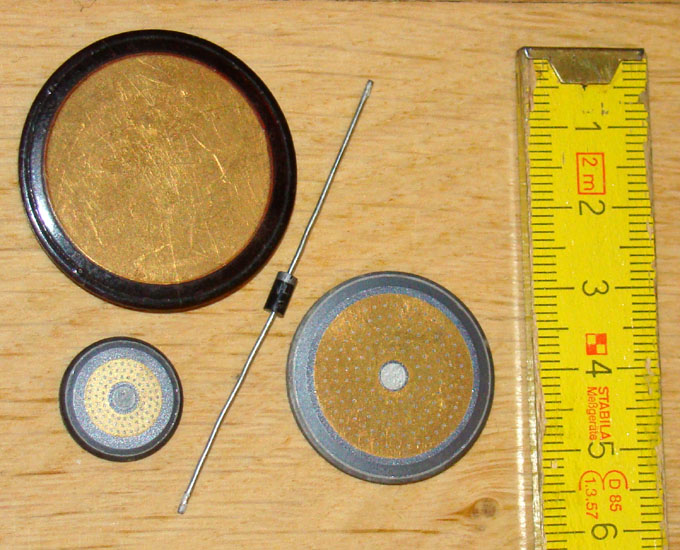
\includegraphics[height=0.45\textheight]{fig/lec05/Thyristor_example_01.jpg}
			\caption{top left: \SI{1000}{\volt}/\SI{200}{\ampere}; bottom left: \SI{1500}{\volt}/\SI{20}{\ampere}; right: \SI{1500}{\volt}/\SI{120}{\ampere}; 1N4007 diode for comparison (source: \href{https://de.wikipedia.org/wiki/Datei:SCR_power_rectifiers.jpg}{Wikimedia Commons}, \href{https://creativecommons.org/publicdomain/zero/1.0/}{CC0~1.0})}
        \end{subfigure}
        \hspace{1cm}
        \begin{subfigure}{0.45\textwidth}
            \centering
            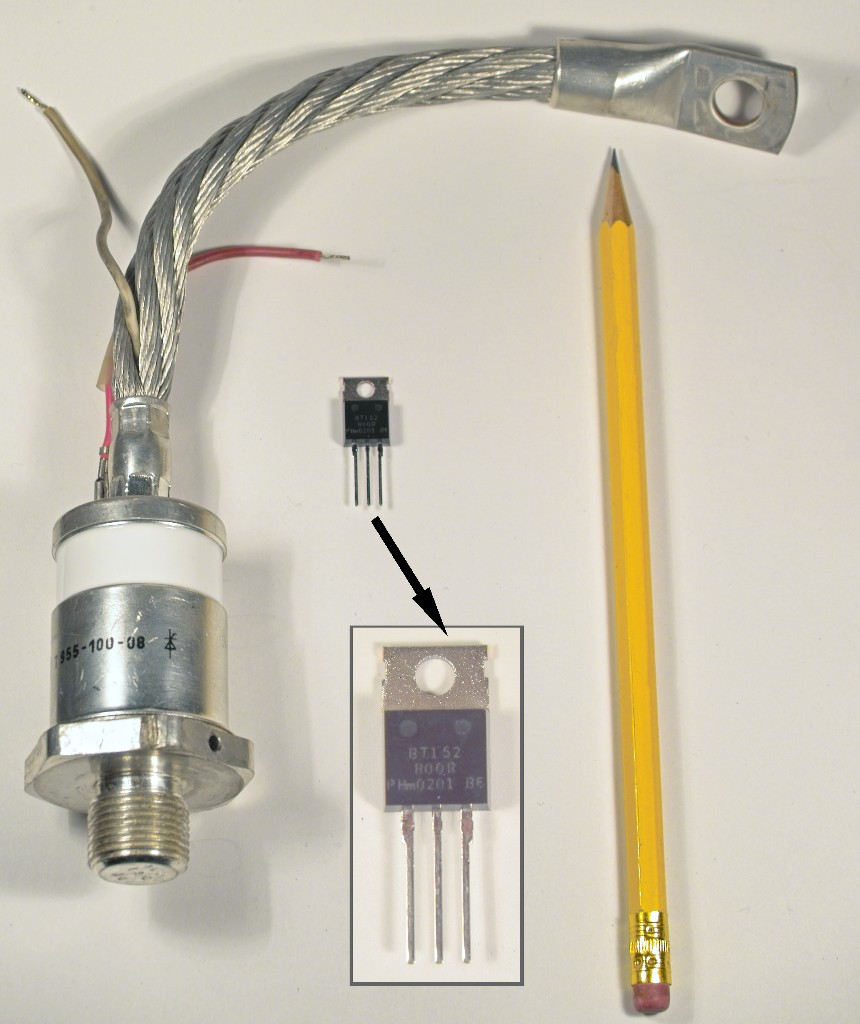
\includegraphics[height=0.45\textheight]{fig/lec05/Thyristor_example_02.jpg}
			\caption{left: \SI{800}{\volt}/\SI{100}{\ampere}; right: \SI{800}{\volt}/\SI{13}{\ampere} (source: \href{https://de.wikipedia.org/wiki/Datei:Thyristors_thyristoren.jpg}{Wikimedia Commons}, Julo, \href{https://creativecommons.org/licenses/by-sa/3.0/deed.de}{CC0~BY-SA~3.0})}
            \vspace{2em}
        \end{subfigure}
        \caption{Thyristor examples with different voltage and current ratings}
        \label{fig:thyristor_examples}
    \end{figure}
\end{frame}

%%%%%%%%%%%%%%%%%%%%%%%%%%%%%%%%%%%%%%%%%%%%%%%%%%%%%%%%%%%%%
%% M1 rectifier comparison %%
%%%%%%%%%%%%%%%%%%%%%%%%%%%%%%%%%%%%%%%%%%%%%%%%%%%%%%%%%%%%%
\begin{frame}
    \frametitle{M1 rectifier comparison}
    \begin{columns}
        \begin{column}{0.5\textwidth}
            \centering
            \begin{circuitikz}[] % M1U diode circuit
                \draw (0,0) to [open, o-o, v = $u_1(t)\hspace{0.5cm}$, voltage = straight] ++(0,-1.5) coordinate (A)
                (0,0) to [short] ++(0.75,0)
                to [diode, l=$D$, v= $u_\mathrm{D}(t)$, voltage = straight]  ++(1.5,0)
                to [short, i=$i_2(t)$] ++(0.75,0)
                to [R, v^= $u_2(t)$, voltage = straight, l_=$R$] ++(0,-1.5) coordinate (B)
                (A) -- (B);
            \end{circuitikz}\\[1em]    
            \begin{tikzpicture}[] % M1U output voltage
                \begin{groupplot}[group style={group size=1 by 2, xticklabels at = edge bottom, vertical sep=1em}, 
                    width=0.85\textwidth,
                    height=0.31\textheight,
                    axis x line=bottom,
	                axis y line=left,
                    xmin=0, xmax=4*pi,
                    ymin=-0.01, ymax=1.15,
                    xtick={0,pi,2*pi, 3*pi, 4*pi},
                    xticklabels={$0$,$\pi$,$2\pi$,$3\pi$,$4\pi$},
                    ytick={-1,0,1},
                    yticklabels={$-\hat{u}_1$,$0$,$\hat{u}_1$},
                    grid=both,
                    ]
                \nextgroupplot[ylabel = {$u_2(\omega t)$}]
                    \addplot[domain=0:pi, samples=50, signalblue, thick, name path = A]{sin(deg(x))};
                    \addplot[domain=pi:2*pi, samples=10, signalblue, thick, name path = B]{0};
                    \addplot[domain=2*pi:3*pi, samples=50, signalblue, thick, name path = C]{sin(deg(x))};
                    \addplot[domain=3*pi:4*pi, samples=10, signalblue, thick, name path = D]{0};
                    \addplot[domain=0:4*pi, samples=10, signalblue, thick,dashed, name path = avg]{1/pi};
                    \node at (axis cs:3*pi/2,1/pi) [anchor=south] {$\overline{u}_2$};
                    \addplot[shadecolor, opacity=0.3] fill between[of=A and avg, soft clip={domain=0:pi}];
                    \addplot[shadecolor, opacity=0.3] fill between[of=B and avg, soft clip={domain=pi:2*pi}];
                    \addplot[shadecolor, opacity=0.3] fill between[of=C and avg, soft clip={domain=2*pi:3*pi}];
                    \addplot[shadecolor, opacity=0.3] fill between[of=D and avg, soft clip={domain=3*pi:4*pi}];

                \nextgroupplot[ylabel = {$u_\mathrm{D}(\omega t)$}, ymin=-1.15, ymax=1.15, height=0.4\textheight, xlabel = {$\omega t$}]
                    \addplot[domain=0:4*pi, samples=50, signalblue, dashed]{sin(deg(x))};
                    \addplot[domain=0:pi, samples=10, signalblue, thick]{0};
                    \addplot[domain=pi:2*pi, samples=50, signalblue, thick]{sin(deg(x))};
                    \addplot[domain=2*pi:3*pi, samples=10, signalblue, thick]{0};
                    \addplot[domain=3*pi:4*pi, samples=50, signalblue, thick]{sin(deg(x))};
                    \node at (axis cs:pi*3/4,1/pi) [anchor=south west] {${u}_1(\omega t)$};
                \end{groupplot}
            \end{tikzpicture}    
        \end{column}
        \begin{column}{0.5\textwidth}
            \centering
            \begin{circuitikz}[] % M1C thyristor circuit
                \draw (0,0) to [open, o-o, v = $u_1(t)\hspace{0.5cm}$, voltage = straight] ++(0,-1.5) coordinate (A)
                (0,0) to [short] ++(0.75,0)
                to [thyristor, voltage = straight, v= $u_\mathrm{T}(t)$, name = T]  ++(1.5,0)
                to [short, i=$i_2(t)$] ++(0.75,0)
                to [R, v^= $u_2(t)$, voltage = straight, l_=$R$] ++(0,-1.5) coordinate (B)
                (A) -- (B);
                \node at (T.gate) [above, xshift=-5mm, yshift=-2mm]{$T$};
            \end{circuitikz}\\[1em]    
            \begin{tikzpicture}[] % M1C output voltage
                \def\a{0.4*pi}
                \begin{groupplot}[group style={group size=1 by 2, xticklabels at = edge bottom, vertical sep=1em}, 
                    width=0.85\textwidth,
                    height=0.31\textheight,
                    axis x line=bottom,
	                axis y line=left,
                    xmin=0, xmax=4*pi,
                    ymin=-0.01, ymax=1.15,
                    xtick={0,pi,2*pi, 3*pi, 4*pi},
                    xticklabels={$0$,$\pi$,$2\pi$,$3\pi$,$4\pi$},
                    ytick={-1,0,1},
                    yticklabels={$-\hat{u}_1$,$0$,$\hat{u}_1$},
                    grid=both,
                    ]
                \nextgroupplot[ylabel = {$u_2(\omega t)$}]
                    \addplot[domain=0:2*pi, samples=150, signalblue, thick, name path = A]{max(sin(deg(x))*max(sign(x-\a),0),0)};
                    \addplot[domain=2*pi:4*pi, samples=150, signalblue, thick, name path = B]{max(sin(deg(x))*max(sign(x-\a-2*pi),0),0)};
                    \addplot[domain=0:4*pi, samples=10, signalblue, thick,dashed, name path = avg]{1/(2*pi)*(1+cos(deg(\a)))};
                    \node at (axis cs:3*pi/2,{1/(2*pi)*(1+cos(deg(\a)))}) [anchor=south] {$\overline{u}_2$};
                    \draw[->] (axis cs:0,0.5) -- node[above]{$\alpha$} (axis cs:\a,0.5) ;
                    \draw[->] (axis cs:2*pi,0.5) -- node[above]{$\alpha$} (axis cs:2*pi+\a,0.5) ;
                    \draw[dashed, thick] (axis cs:2*pi,0) -- (axis cs:2*pi,1);
                    \addplot[shadecolor, opacity=0.3] fill between[of=A and avg, soft clip={domain=0:2*pi}];
                    \addplot[shadecolor, opacity=0.3] fill between[of=B and avg, soft clip={domain=2*pi:4*pi}];


                \nextgroupplot[ylabel = {$u_\mathrm{T}(\omega t)$}, ymin=-1.15, ymax=1.15, height=0.4\textheight, xlabel = {$\omega t$}]
                    \addplot[domain=0:4*pi, samples=50, signalblue, dashed]{sin(deg(x))};
                    \addplot[domain=0:2*pi, samples=150, signalblue, thick]{max(sin(deg(x))*max(-sign(x-\a),0),0) + sin(deg(x))*max(sign(x-pi),0)};
                    \addplot[domain=2*pi:4*pi, samples=150, signalblue, thick]{max(sin(deg(x))*max(-sign(x-\a-2*pi),0),0) + sin(deg(x))*max(sign(x-3*pi),0)};
                    \node at (axis cs:pi*3/4,1/pi) [anchor=south west] {${u}_1(\omega t)$};
                \end{groupplot}
            \end{tikzpicture}          
        \end{column}
    \end{columns}
\end{frame}

%%%%%%%%%%%%%%%%%%%%%%%%%%%%%%%%%%%%%%%%%%%%%%%%%%%%%%%%%%%%%
%% Half-cycle rectification / M1C circuit %%
%%%%%%%%%%%%%%%%%%%%%%%%%%%%%%%%%%%%%%%%%%%%%%%%%%%%%%%%%%%%%
\subsection{M1C circuit} 

%%%%%%%%%%%%%%%%%%%%%%%%%%%%%%%%%%%%%%%%%%%%%%%%%%%%%%%%%%%%%
%% M1C rectifier %%
%%%%%%%%%%%%%%%%%%%%%%%%%%%%%%%%%%%%%%%%%%%%%%%%%%%%%%%%%%%%%
\begin{frame}
    \frametitle{M1C rectifier}
    The \hl{average output voltage} of the M1C circuit, i.e., the M1 rectifier with a thyristor, for a resistive load is given by
    \begin{equation}
        \overline{u}_2 = \frac{1}{2\pi} \int_{\alpha}^{\pi} \hat{u}_1 \sin(\omega t) \mathrm{d} \omega t = \frac{\hat{u}_1}{2\pi} \left[ -\cos(\omega t) \right]_{\alpha}^{\pi} = \frac{\hat{u}_1}{2\pi} \left( 1 + \cos(\alpha) \right). 
    \end{equation}
    Here, $\alpha$ denotes the phase angle at which the thyristor is triggered (aka \hl{firing angle}). In the M1C case, the feasible range for $\alpha$ is $[0,\nicefrac{\pi}{2}]$ applies as the thyristor requires a positive forward voltage to start conducting, that is, if $u_\mathrm{T}<0$ a firing impulse would not change its conduction state. The \hl{RMS value} of the output voltage is given by
    The \hl{RMS value} of the output voltage is given by
    \begin{equation}
        U_2 = \sqrt{\frac{1}{2\pi} \int_{\alpha}^{\pi} \hat{u}_1^2 \sin^2(\omega t) \mathrm{d} \omega t} =   \ldots = \frac{\hat{u}_1}{2} \sqrt{\frac{\pi - \alpha + \sin(\alpha)\cos(\alpha)}{\pi}}.
    \end{equation}
    In contrast to the M1U rectifier from \eqref{eq:u2_M1U_avg}, the \hl{M1C rectifier allows for controlling the output voltage} by adjusting the firing angle $\alpha$.
\end{frame}

%%%%%%%%%%%%%%%%%%%%%%%%%%%%%%%%%%%%%%%%%%%%%%%%%%%%%%%%%%%%%
%% M1C rectifier: Fourier series %%
%%%%%%%%%%%%%%%%%%%%%%%%%%%%%%%%%%%%%%%%%%%%%%%%%%%%%%%%%%%%%
\begin{frame}
    \frametitle{M1C rectifier: Fourier series}
    \onslide<1->{The \hl{Fourier coefficients} of the output voltage $u_2(t)$ for the M1C converter are}
    \begin{equation}
        \begin{split}
            \onslide<1->{a^{(0)} &= \frac{1}{\pi} \int_0^{2\pi} u_2(t) \mathrm{d} \omega t = \frac{1}{\pi} \int_{\alpha}^{\pi} \hat{u}_1 \sin(\omega t) \mathrm{d}\omega t} \onslide<2->{= 2 \overline{u}_2= \frac{\hat{u}_1}{\pi}(1+\cos(\alpha)),}\\
            \onslide<3->{a^{(k)} &= \frac{1}{\pi} \int_{0}^{2\pi} u_2(t) \cos(k\omega t) \mathrm{d}\omega t  = \frac{1}{\pi} \int_{\alpha}^{\pi} \hat{u}_1 \sin(\omega t) \cos(k\omega t) \mathrm{d}\omega t}=\ldots \\ & \onslide<4->{=  \begin{cases}\frac{\hat{u}_1}{\pi}\frac{2}{1-k^2}, & k=1\\ \frac{1}{2\pi} \left( \frac{\cos(\alpha(k-1)) + \cos(k\pi)}{k-1} - \frac{\cos(\alpha(k+1)) + \cos(k\pi)}{k+1} \right), & k \geq 2. \end{cases} }\\
            \onslide<7->{b^{(k)} &= \frac{1}{\pi} \int_{0}^{2\pi} u_2(t) \sin(k\omega t) \mathrm{d}\omega t = \frac{1}{\pi} \int_{\alpha}^{\pi} \hat{u}_1 \sin(\omega t) \sin(k\omega t) \mathrm{d}\omega t}=\ldots \\ &\onslide<8->{= \begin{cases} \frac{-\alpha + \pi + \cos(\alpha)\sin(\alpha)}{2\pi}, & k =1,\\ \frac{1}{2\pi} \left( \frac{\sin(\alpha(k-1)) + \sin(k\pi)}{k-1} - \frac{\sin(\alpha(k+1)) + \sin(k\pi)}{k+1} \right), & k \geq 2. \end{cases}}
        \end{split}
        \label{eq:u2_M1C_Fourier}
    \end{equation}
    \onslide<10->{In contrast to the M1U rectifier, one can observe additional harmonic components due to additional distortion of the output voltage caused by the thyristor switching.}
\end{frame}

%%%%%%%%%%%%%%%%%%%%%%%%%%%%%%%%%%%%%%%%%%%%%%%%%%%%%%%%%%%%%
%% M2C controllable rectifier circuit  %%
%%%%%%%%%%%%%%%%%%%%%%%%%%%%%%%%%%%%%%%%%%%%%%%%%%%%%%%%%%%%%
\begin{frame}[c]
    \frametitle{M2C converter}
    \begin{figure}
           \begin{circuitikz}[baseline=(current bounding box.center)]
            \draw (0,0) node[transformer core](T){$N_1:N_2$}
            (T.inner dot A1) node[circ]{}
            (T.inner dot B1) node[circ]{}
            (T.A1) to [short] ++(0,1) to [short, -o, i<_=$i_1(t)$] ++(-1,0) coordinate (A1)
            (T.A2) to [short] ++(0,-1) to [short, -o] ++(-1,0) coordinate (A2)
            (T.B1) to [short] ++(0, 1) coordinate (B1)
            (T.B2) to [short] ++(0,-1) coordinate (B2);
            \draw (A1) to [open, v=$u_1(t)\hspace{0.5cm}$, voltage = straight] (A2); 
            \draw (B1) to [thyristor, name=T1] ++(2.0,0) coordinate (C1)
            (B2) to [thyristor, name=T2] ++(2.0,0)
            to [crossing, -*, mirror] (C1)
            to [short, i=$i_2(t)$] ++(1.0,0) coordinate (D)
            to [R, v^= $u_2(t)$, voltage = straight, l_=$R$] (T-L2.midtap -| D)
            to [short] (T-L2.midtap);
            \draw let \p1 = (B1), \p2 = (T-L2.midtap) in (\x1 + 0.5cm, \y1) to [open, v^=$\hspace{0.5cm}{u_\mathrm{s,1}(t)}$, voltage = straight] (\x1 + 0.5cm, \y2);
            \draw let \p1 = (B2), \p2 = (T-L2.midtap) in (\x1 + 0.5cm, \y1) to [open, v=$\hspace{0.5cm}{u_\mathrm{s,2}(t)}$, voltage = straight] (\x1 + 0.5cm, \y2);
            \node at (T1.gate) [above, xshift=-5mm, yshift=-2mm]{$T_1$};
            \node at (T2.gate) [below, xshift=-5mm, yshift=-7mm]{$T_2$};
        \end{circuitikz}%
        \hspace{0.25cm}
        \begin{tikzpicture}[baseline=(current bounding box.center)] % M1C output voltage
            \def\a{0.4*pi}
            \begin{groupplot}[group style={group size=1 by 2, xticklabels at = edge bottom, vertical sep=1em}, 
                width=0.38\textwidth,
                height=0.4\textheight,
                axis x line=bottom,
                axis y line=left,
                xmin=0, xmax=4*pi,
                ymin=-1.15, ymax=1.15,
                xtick={0,pi,2*pi, 3*pi, 4*pi},
                xticklabels={$0$,$\pi$,$2\pi$,$3\pi$,$4\pi$},
                ytick={-1,0,1},
                yticklabels={$-\hat{u}_\mathrm{s}$,$0$,$\hat{u}_\mathrm{s}$},
                grid=both,
                clip=false
                ]
            \nextgroupplot[ylabel = {$u_2(\omega t)$}]
                \addplot[domain=0:pi, samples=50, signalblue, thick, name path = A]{(x < \a) * 0 + (x > \a) * sin(deg(x))};
                \addplot[domain=pi:2*pi, samples=50, signalblue, thick, name path = B]{(x - pi < \a) * 0 + (x - pi > \a) * -sin(deg(x))};
                \addplot[domain=2*pi:3*pi, samples=50, signalblue, thick, name path = C]{(x - 2*pi < \a) * 0 + (x - 2*pi > \a) * sin(deg(x))};
                \addplot[domain=3*pi:4*pi, samples=50, signalblue, thick, name path = D]{(x - 3*pi < \a) * 0 + (x - 3*pi > \a) * -sin(deg(x))};
                \addplot[domain=0:4*pi, samples=10, signalblue, thick,dashed, name path = avg]{1/(pi)*(1+cos(deg(\a)))};
                \node at (axis cs:3*pi/2+0.4,{1/(pi)*(1+cos(deg(\a)))}) [anchor=north] {$\overline{u}_2$};
                \draw[->] (axis cs:0,1) -- node[above]{$\alpha$} (axis cs:\a,1) ;
                \draw[->] (axis cs:2*pi,1) -- node[above]{$\alpha$} (axis cs:2*pi+\a,1) ;
                \draw[dashed, thick] (axis cs:2*pi,0) -- (axis cs:2*pi,1);
                \addplot[domain=0:4*pi, samples=50, signalgreen, dashed]{sin(deg(x))};
                \addplot[domain=0:4*pi, samples=50, signalbrown, dashed]{-sin(deg(x))};
                \node at (axis cs:pi*2.5,-0.75) [anchor=south, signalbrown] {$u_{s,2}$};
                \node at (axis cs:pi*3.5,-0.75) [anchor=south, signalgreen] {$u_{s,1}$};
                \addplot[shadecolor, opacity=0.3] fill between[of=A and avg, soft clip={domain=0:pi}];
                \addplot[shadecolor, opacity=0.3] fill between[of=B and avg, soft clip={domain=pi:2*pi}];
                \addplot[shadecolor, opacity=0.3] fill between[of=C and avg, soft clip={domain=2*pi:3*pi}];
                \addplot[shadecolor, opacity=0.3] fill between[of=D and avg, soft clip={domain=3*pi:4*pi}];


            \nextgroupplot[ylabel = {$u_\mathrm{T}(\omega t)$}, xlabel = {$\omega t$}, ymin=-2.15, ytick={-2, -1,0,1}, yticklabels={$-2\hat{u}_\mathrm{s}$, $-\hat{u}_\mathrm{s}$,$0$,$\hat{u}_\mathrm{s}$}, height=0.5\textheight]
                \node at (axis cs:\a,0.5) [signalgreen, right, inner sep=1pt] {${u}_{T_1}$};
                \node at (axis cs:\a+pi,0.5) [signalbrown, right, inner sep=1pt] {${u}_{T_2}$};
                \addplot[domain=0:pi, samples=50, signalgreen, thick]{(x < \a) * sin(deg(x)) + (x > \a) * 0};
                \addplot[domain=0:pi, samples=50, signalbrown, thick]{-sin(deg(x)) + (x > \a) * -sin(deg(x))};
                \addplot[domain=pi:2*pi, samples=50, signalbrown, thick]{(x -pi < \a) * -sin(deg(x)) + (x-pi > \a) * 0};
                \addplot[domain=pi:2*pi, samples=50, signalgreen, thick]{sin(deg(x)) + (x -pi > \a) * sin(deg(x))};
                \addplot[domain=2*pi:3*pi, samples=50, signalgreen, thick]{(x -2*pi < \a) * sin(deg(x)) + (x  -2*pi > \a) * 0};
                \addplot[domain=2*pi:3*pi, samples=50, signalbrown, thick]{-sin(deg(x)) + (x  -2*pi > \a) * -sin(deg(x))};
                \addplot[domain=3*pi:4*pi, samples=50, signalbrown, thick]{(x - 3*pi < \a) * -sin(deg(x)) + (x - 3*pi > \a) * 0};
                \addplot[domain=3*pi:4*pi, samples=50, signalgreen, thick]{sin(deg(x)) + (x - 3*pi > \a) * sin(deg(x))};
            \end{groupplot}
        \end{tikzpicture}   
        \caption{M2C topology (aka \hl{two-pulse mid-point converter}) with center-tapped transformer and a resistive load}
        \label{fig:M2C_topology}
    \end{figure}
\end{frame}

%%%%%%%%%%%%%%%%%%%%%%%%%%%%%%%%%%%%%%%%%%%%%%%%%%%%%%%%%%%%%
%% M2C circuit %%
%%%%%%%%%%%%%%%%%%%%%%%%%%%%%%%%%%%%%%%%%%%%%%%%%%%%%%%%%%%%%
\subsection{M2C circuit} 

%%%%%%%%%%%%%%%%%%%%%%%%%%%%%%%%%%%%%%%%%%%%%%%%%%%%%%%%%%%%%
%% M2C converter: resistive load  %%
%%%%%%%%%%%%%%%%%%%%%%%%%%%%%%%%%%%%%%%%%%%%%%%%%%%%%%%%%%%%%
\begin{frame}
    \frametitle{M2C converter: resistive load}
    The \hl{average output voltage} of the M2C converter for a resistive load is given by
    \begin{equation}
        \overline{u}_2 = \frac{1}{\pi} \int_{\alpha}^{\pi} \hat{u}_\mathrm{s} \sin(\omega t) \mathrm{d} \omega t = \frac{\hat{u}_\mathrm{s}}{\pi} \left[ -\cos(\omega t) \right]_{\alpha}^{\pi} = \frac{\hat{u}_\mathrm{s}}{\pi} \left( 1 + \cos(\alpha) \right).
    \end{equation}
    The \hl{RMS value} of the output voltage results in
    \begin{equation}
        U_2 = \sqrt{\frac{1}{\pi} \int_{\alpha}^{\pi} \hat{u}_\mathrm{s}^2 \sin^2(\omega t) \mathrm{d} \omega t} =   \ldots = \frac{\hat{u}_\mathrm{s}}{\sqrt{2}} \sqrt{\frac{\pi - \alpha + \sin(\alpha)\cos(\alpha)}{\pi}}.
    \end{equation}
    The primary to secondary voltage ratio of the center-tapped transformer yields
    \begin{equation*}
        \frac{\hat{u}_\mathrm{s}}{\hat{u}_1} = \frac{1}{2}\frac{N_2}{N_1}.
    \end{equation*}
    It should be noted that in the case of a resistive load, the M2C's output voltage is always positive for the M2C's feasible firing angle range $\alpha \in [0,\pi]$.
\end{frame}

%%%%%%%%%%%%%%%%%%%%%%%%%%%%%%%%%%%%%%%%%%%%%%%%%%%%%%%%%%%%%
%% M2C converter with an output filter  %%
%%%%%%%%%%%%%%%%%%%%%%%%%%%%%%%%%%%%%%%%%%%%%%%%%%%%%%%%%%%%%
\begin{frame}[c]
    \frametitle{M2C converter with an output filter}
    \begin{figure}
           \begin{circuitikz}[baseline=(current bounding box.center)]
            \draw (0,0) node[transformer core](T){$N_1:N_2$}
            (T.inner dot A1) node[circ]{}
            (T.inner dot B1) node[circ]{}
            (T.A1) to [short] ++(0,1) to [short, -o, i<_=$i_1(t)$] ++(-1,0) coordinate (A1)
            (T.A2) to [short] ++(0,-1) to [short, -o] ++(-1,0) coordinate (A2)
            (T.B1) to [short] ++(0, 1) coordinate (B1)
            (T.B2) to [short] ++(0,-1) coordinate (B2);
            \draw (A1) to [open, v=$u_1(t)\hspace{0.5cm}$, voltage = straight] (A2); 
            \draw (B1) to [thyristor, name=T1] ++(2.0,0) coordinate (C1)
            (B2) to [thyristor, name=T2] ++(2.0,0)
            to [crossing, -*, mirror] (C1)
            to [short] ++(0.5,0) coordinate (us)
            to [L, l=$L$] ++(2,0) 
            to [short] ++(0.5,0) coordinate (D)
            to [short, i=$i_2(t)$] ++(1.5,0)
            to [open, v^= $\hspace{0.5cm}u_2(t)$, voltage = straight, o-o] (T-L2.midtap -| \tikztostart)
            to [short] (\tikztostart -| D)
            (D) to [C, voltage = straight, l=$C$, *-*] (T-L2.midtap -| D)
            to [short] (T-L2.midtap);
            \draw (us) to [open, v^=$\hspace{0.5cm}u_\mathrm{s}(t)$, voltage = straight] (T-L2.midtap -| us);
            \draw let \p1 = (B1), \p2 = (T-L2.midtap) in (\x1 + 0.5cm, \y1) to [open, v^=$\hspace{0.5cm}{u_\mathrm{s,1}(t)}$, voltage = straight] (\x1 + 0.5cm, \y2);
            \draw let \p1 = (B2), \p2 = (T-L2.midtap) in (\x1 + 0.5cm, \y1) to [open, v=$\hspace{0.5cm}{u_\mathrm{s,2}(t)}$, voltage = straight] (\x1 + 0.5cm, \y2);
            \node at (T1.gate) [above, xshift=-5mm, yshift=-2mm]{$T_1$};
            \node at (T2.gate) [below, xshift=-5mm, yshift=-7mm]{$T_2$};
        \end{circuitikz}%
        \caption{M2C converter with an output filter assuming $u_2(t)=U_2=\mbox{const.}$}
        \label{fig:M2C_output_filter}
    \end{figure}
\end{frame}

%%%%%%%%%%%%%%%%%%%%%%%%%%%%%%%%%%%%%%%%%%%%%%%%%%%%%%%%%%%%%
%% M2C converter with an output filter  %%
%%%%%%%%%%%%%%%%%%%%%%%%%%%%%%%%%%%%%%%%%%%%%%%%%%%%%%%%%%%%%
\begin{frame}[c]
    \frametitle{M2C converter with an output filter (cont.)}
    \begin{figure}
        \begin{tikzpicture} % M1C output voltage
            \tikzmath{
                    real \a, \iLavg1, \iLavg1, \Lw, \u1, \uc1, \iLs1, \iLs2, \b, \adcm;
                    \a = 0.3*pi; %firing angle
                    \Lw = 2; %angular frequency times inductance
                    \u1 = 1; %Input voltage amplitude
                    \uc1 = 2*\u1/pi*cos(deg(\a)); %output voltage for CCM
                    \iLs1 = 0.6; %current initial value for CCM
                    \iLs2 = -1/\Lw*(-\uc1*\a + \u1*(cos(deg(\a))-1)); %current initial value for BCM
                    \iLavg1 = \iLs1 + 1/(\Lw*pi)*(-\uc1*(pi^2/2) + \u1*(2*sin(deg(\a)) - \a + (2*cos(deg(\a))-1)*(pi-\a))); %current average value for CCM
                    \iLavg2 = \iLs2 + 1/(\Lw*pi)*(-\uc1*(pi^2/2) + \u1*(2*sin(deg(\a)) - \a + (2*cos(deg(\a))-1)*(pi-\a))); %current average value for BCM
                    \b = 0.8*pi; %conduction interval for DCM
                    \adcm = 0.4*pi; %firing angle for DCM (\b + \adcm must be greater than pi for corret visualization)
                    \ucdcm = -1/\b*(\u1*(cos(deg(\adcm+\b))-cos(deg(\adcm)))); %output voltage for DCM
                    \iLavg3 = 1/(\Lw*pi)*(-\u1*(sin(deg(\adcm+\b))-sin(deg(\adcm))-cos(deg(\adcm))*\b) - \ucdcm*(\b^2/2)); %current average value for DCM
                }
            \begin{groupplot}[group style={group size=3 by 2, xticklabels at = edge bottom, vertical sep=1em, yticklabels at = edge left, horizontal sep = 1em}, 
                width=0.38\textwidth,
                height=0.34\textheight,
                axis x line=bottom,
                axis y line=left,
                xmin=0, xmax=2*pi,
                ymin=-1.15, ymax=1.15,
                xtick={0, pi/2, pi, 3*pi/2, 2*pi},
                xticklabels={$0$,$\frac{1}{2}\pi$, $\pi$,$\frac{3}{2}\pi$, $2\pi$},
                ytick={-1, -1/2, 0,1/2, 1},
                yticklabels={$-\hat{u}_\mathrm{s}$, ,$0$, ,$\hat{u}_\mathrm{s}$},
                grid=both,
                clip=false
                ]
            \nextgroupplot[ylabel = {$u_\mathrm{s}(\omega t)$}, title=CCM, height=0.475\textheight] % voltage CCM
                \addplot[domain=0:pi, samples=50, signalblue, thick, name path = A1]{(x < \a) * -sin(deg(x)) + (x > \a) * sin(deg(x))};
                \addplot[domain=pi:2*pi, samples=50, signalblue, thick, name path = B1]{(x - pi < \a) * sin(deg(x)) + (x - pi > \a) * -sin(deg(x))};
                \addplot[domain=0:2*pi, samples=10, signalblue, thick,dashed, name path = avg1]{2/(pi)*(cos(deg(\a)))};
                \node at (axis cs:3*pi/2+0.4,{2/(pi)*(cos(deg(\a)))}) [anchor=north] {$\overline{u}_2$};
                \draw[->] (axis cs:0,1) -- node[above]{$\alpha$} (axis cs:\a,1) ;
                \draw[->] (axis cs:pi,1) -- node[above]{$\alpha$} (axis cs:pi+\a,1) ;
                \draw[dashed, thick] (axis cs:pi,0) -- (axis cs:pi,1);
                \addplot[domain=0:2*pi, samples=50, signalgreen, dashed]{sin(deg(x))};
                \addplot[domain=0:2*pi, samples=50, signalbrown, dashed]{-sin(deg(x))};
                \node at (axis cs:pi*3/4,-0.75) [signalbrown, fill=white,inner sep=1pt] {$u_{s,2}$};
                \node at (axis cs:pi*7/4,-0.75) [signalgreen, fill=white,inner sep=1pt] {$u_{s,1}$};
                \addplot[shadecolor, opacity=0.3] fill between[of=A1 and avg1, soft clip={domain=0:pi}];
                \addplot[shadecolor, opacity=0.3] fill between[of=B1 and avg1, soft clip={domain=pi:2*pi}];

            \nextgroupplot[title=BCM, height=0.475\textheight] % voltage BCM
                \addplot[domain=0:pi, samples=50, signalblue, thick, name path = A2]{(x < \a) * -sin(deg(x)) + (x > \a) * sin(deg(x))};
                \addplot[domain=pi:2*pi, samples=50, signalblue, thick, name path = B2]{(x - pi < \a) * sin(deg(x)) + (x - pi > \a) * -sin(deg(x))};
                \addplot[domain=0:2*pi, samples=10, signalblue, thick,dashed, name path = avg2]{2/(pi)*(cos(deg(\a)))};
                \node at (axis cs:3*pi/2+0.4,{2/(pi)*(cos(deg(\a)))}) [anchor=north] {$\overline{u}_2$};
                \draw[->] (axis cs:0,1) -- node[above]{$\alpha$} (axis cs:\a,1) ;
                \draw[->] (axis cs:pi,1) -- node[above]{$\alpha$} (axis cs:pi+\a,1) ;
                \draw[dashed, thick] (axis cs:pi,0) -- (axis cs:pi,1);
                \addplot[domain=0:2*pi, samples=50, signalgreen, dashed]{sin(deg(x))};
                \addplot[domain=0:2*pi, samples=50, signalbrown, dashed]{-sin(deg(x))};
                \node at (axis cs:pi*3/4,-0.75) [signalbrown, fill=white,inner sep=1pt] {$u_{s,2}$};
                \node at (axis cs:pi*7/4,-0.75) [signalgreen, fill=white,inner sep=1pt] {$u_{s,1}$};
                \addplot[shadecolor, opacity=0.3] fill between[of=A2 and avg2, soft clip={domain=0:pi}];
                \addplot[shadecolor, opacity=0.3] fill between[of=B2 and avg2, soft clip={domain=pi:2*pi}];

            \nextgroupplot[title=DCM, height=0.475\textheight] % voltage DCM
                \addplot[domain=0:2*pi, samples=200, signalblue, thick, name path = A3]{(x < \adcm +\b - pi) * sin(deg(x+pi)) + (x > \adcm + \b -pi) * (x < \adcm) * \ucdcm + (x > \adcm)* (x < \adcm + \b) * sin(deg(x)) + (x > \adcm + \b) * (x < \adcm + pi) * \ucdcm + (x > \adcm + pi) * sin(deg(x-pi))};
                \addplot[domain=0:2*pi, samples=10, signalblue, thick,dashed, name path = avg3]{\ucdcm};
                \node at (axis cs:3*pi/2+0.4,\ucdcm) [anchor=north] {$\overline{u}_2$};
                \addplot[domain=0:2*pi, samples=50, signalgreen, dashed]{sin(deg(x))};
                \addplot[domain=0:2*pi, samples=50, signalbrown, dashed]{-sin(deg(x))};
                \node at (axis cs:pi*3/4,-0.75) [signalbrown, fill=white,inner sep=1pt] {$u_{s,2}$};
                \node at (axis cs:pi*7/4,-0.75) [signalgreen, fill=white,inner sep=1pt] {$u_{s,1}$};
                \draw[->] (axis cs:0,1) -- node[above]{$\alpha$} (axis cs:\adcm,1) ;
                \draw[->] (axis cs:pi,1) -- node[above]{$\alpha$} (axis cs:pi+\adcm,1) ;
                \draw[dashed, thick] (axis cs:pi,0) -- (axis cs:pi,1);
                \addplot[shadecolor, opacity=0.3] fill between[of=A3 and avg3, soft clip={domain=0:2*pi}];
                


            \nextgroupplot[ylabel = {$i_\mathrm{L}(\omega t)$}, xlabel = {$\omega t$}, ymin=-0.01, ytick={0, 1/2, 1}, yticklabels={$0$, } ] %current CCM
                \addplot[domain=0:\a, samples=50, signalred, thick, name path = Ai1]{1/\Lw*(-\uc1*x + \u1*(cos(deg(x))-1))+\iLs1};
                \addplot[domain=\a:pi, samples=50, signalred, thick, name path = Bi1]{1/\Lw*(-\uc1*\a + \u1*(cos(deg(\a))-1))+\iLs1 + 1/\Lw*(\u1*(-cos(deg(x))+cos(deg(\a))) - \uc1*(x-\a))};
                \addplot[domain=pi:pi+\a, samples=50, signalred, thick, name path = Ci1]{1/\Lw*(-\uc1*(x-pi) + \u1*(cos(deg(x - pi))-1))+\iLs1};
                \addplot[domain=pi+\a:2*pi, samples=50, signalred, thick, name path = Di1]{1/\Lw*(-\uc1*\a + \u1*(cos(deg(\a))-1))+\iLs1 + 1/\Lw*(\u1*(-cos(deg(x-pi))+cos(deg(\a))) - \uc1*(x-\a-pi))};
                \addplot[domain=0:2*pi, samples=10, signalred, thick,dashed, name path = avgi1]{\iLavg1};
                \draw[<->] (axis cs:\a,0.75) -- node[above, fill = white]{$\beta=\pi$} (axis cs:\a+pi,0.75) ;
                \addplot[shadecolor, opacity=0.3] fill between[of=Ai1 and avgi1, soft clip={domain=0:\a}];
                \addplot[shadecolor, opacity=0.3] fill between[of=Bi1 and avgi1, soft clip={domain=\a:pi}];
                \addplot[shadecolor, opacity=0.3] fill between[of=Ci1 and avgi1, soft clip={domain=pi:pi+\a}];
                \addplot[shadecolor, opacity=0.3] fill between[of=Di1 and avgi1, soft clip={domain=pi+\a:2*pi}];

            \nextgroupplot[xlabel = {$\omega t$}, ymin=-0.01, ytick={0, 1/2, 1}, yticklabels={ } ] %current BCM
                \addplot[domain=0:\a, samples=50, signalred, thick, name path = Ai2]{1/\Lw*(-\uc1*x + \u1*(cos(deg(x))-1))+\iLs2};
                \addplot[domain=\a:pi, samples=50, signalred, thick, name path = Bi2]{1/\Lw*(-\uc1*\a + \u1*(cos(deg(\a))-1))+\iLs2 + 1/\Lw*(\u1*(-cos(deg(x))+cos(deg(\a))) - \uc1*(x-\a))};
                \addplot[domain=pi:pi+\a, samples=50, signalred, thick, name path = Ci2]{1/\Lw*(-\uc1*(x-pi) + \u1*(cos(deg(x - pi))-1))+\iLs2};
                \addplot[domain=pi+\a:2*pi, samples=50, signalred, thick, name path = Di2]{1/\Lw*(-\uc1*\a + \u1*(cos(deg(\a))-1))+\iLs2 + 1/\Lw*(\u1*(-cos(deg(x-pi))+cos(deg(\a))) - \uc1*(x-\a-pi))};
                \addplot[domain=0:2*pi, samples=10, signalred, thick,dashed, name path = avgi2]{\iLavg2};
                \draw[<->] (axis cs:\a,0.6) -- node[above, fill = white]{$\beta=\pi$} (axis cs:\a+pi,0.6) ;
                \addplot[shadecolor, opacity=0.3] fill between[of=Ai2 and avgi2, soft clip={domain=0:\a}];
                \addplot[shadecolor, opacity=0.3] fill between[of=Bi2 and avgi2, soft clip={domain=\a:pi}];
                \addplot[shadecolor, opacity=0.3] fill between[of=Ci2 and avgi2, soft clip={domain=pi:pi+\a}];
                \addplot[shadecolor, opacity=0.3] fill between[of=Di2 and avgi2, soft clip={domain=pi+\a:2*pi}];

            \nextgroupplot[xlabel = {$\omega t$}, ymin=-0.01, ytick={0, 1/2, 1}, yticklabels={} ] %current DCM
                \addplot[domain=\adcm:\adcm+\b, samples=50, signalred, thick, name path = Ai3]{1/\Lw*(-\ucdcm*(x-\adcm) - \u1*(cos(deg(x))-cos(deg(\adcm))))};
                \addplot[domain=0:\adcm+\b-pi, samples=50, signalred, thick, name path = Bi3]{1/\Lw*(-\ucdcm*(x-\adcm+pi) - \u1*(cos(deg(x+pi))-cos(deg(\adcm))))};
                \addplot[domain=\adcm+pi:2*pi, samples=50, signalred, thick, name path = Ci3]{1/\Lw*(-\ucdcm*(x-\adcm-pi) - \u1*(cos(deg(x-pi))-cos(deg(\adcm))))};
                \addplot[domain=\adcm+\b:\adcm+pi, samples=50, signalred, thick, name path = Di3]{0};
                \addplot[domain=\adcm+\b-pi:\adcm, samples=50, signalred, thick, name path = Ei3]{0};
                \addplot[domain=0:2*pi, samples=10, signalred, thick,dashed, name path = avgi3]{\iLavg3};
                \draw[<->] (axis cs:\adcm,0.5) -- node[above, fill = white]{$\beta<\pi$} (axis cs:\adcm+\b,0.5) ;
                \addplot[shadecolor, opacity=0.3] fill between[of=Ai3 and avgi3, soft clip={domain=\adcm:\adcm+\b}];
                \addplot[shadecolor, opacity=0.3] fill between[of=Bi3 and avgi3, soft clip={domain=0:\adcm+\b-pi}];
                \addplot[shadecolor, opacity=0.3] fill between[of=Ci3 and avgi3, soft clip={domain=\adcm+pi:2*pi}];
                \addplot[shadecolor, opacity=0.3] fill between[of=Di3 and avgi3, soft clip={domain=\adcm+\b:\adcm+pi}];
                \addplot[shadecolor, opacity=0.3] fill between[of=Ei3 and avgi3, soft clip={domain=\adcm+\b-pi:\adcm}];

            \end{groupplot}
        \end{tikzpicture}   
        \caption{M2C topology with an output filter and different average load currents}
        \label{fig:M2C_different_loads}
    \end{figure}
\end{frame}

%%%%%%%%%%%%%%%%%%%%%%%%%%%%%%%%%%%%%%%%%%%%%%%%%%%%%%%%%%%%%
%% M2C converter with an output filter  %%
%%%%%%%%%%%%%%%%%%%%%%%%%%%%%%%%%%%%%%%%%%%%%%%%%%%%%%%%%%%%%
\begin{frame}[c]
    \frametitle{M2C converter with an output filter (cont.)}
    Due to the output filter, the secondary voltage $u_\mathrm{s}(t)$ can become negative since the current flow is maintained by the inductor and, therefore, a thyristor is remaining in the conducting state (until the other thyristor is triggered). The \hl{average output voltage in CCM (and BCM)} is given by
    \begin{equation}
        \begin{split}
            \overline{u}_2 &= \frac{1}{\pi} \int_{\alpha}^{\alpha+\pi} \hat{u}_\mathrm{s} \sin(\omega t) \mathrm{d} \omega t = \frac{\hat{u}_\mathrm{s}}{\pi} \left[ -\cos(\omega t) \right]_{\alpha}^{\alpha+\pi} = \frac{\hat{u}_\mathrm{s}}{\pi} \left(-\cos(\alpha+\pi) +\cos(\alpha)\right)\\
             &= \hat{u}_\mathrm{s}\frac{2}{\pi} \cos(\alpha).
        \end{split}
        \label{eq:u2_avg_M2C_CCM}
    \end{equation}
    In DCM the \hl{conduction interval} $\beta$ is less than $\pi$ and the \hl{average output voltage} is given by
    \begin{equation}
        \begin{split}
        \overline{u}_2 &= \frac{1}{\pi} \int_{\alpha}^{\alpha+\beta} \hat{u}_\mathrm{s} \sin(\omega t) \mathrm{d} \omega t = \frac{\hat{u}_\mathrm{s}}{\pi} \left[ -\cos(\omega t) \right]_{\alpha}^{\alpha+\beta} = \frac{\hat{u}_\mathrm{s}}{\pi} \left(\cos(\alpha)-\cos(\alpha+\beta)\right)\\
                       &= \hat{u}_\mathrm{s}\frac{2}{\pi}\sin\left(\frac{\beta}{2}\right)\sin\left(\alpha + \frac{\beta}{2}\right).
    \end{split}
    \end{equation}
\end{frame}

%%%%%%%%%%%%%%%%%%%%%%%%%%%%%%%%%%%%%%%%%%%%%%%%%%%%%%%%%%%%%
%% M2C converter with an active load  %%
%%%%%%%%%%%%%%%%%%%%%%%%%%%%%%%%%%%%%%%%%%%%%%%%%%%%%%%%%%%%%
\begin{frame}[c]
    \frametitle{M2C converter with an active load}
    Analyzing \eqref{eq:u2_avg_M2C_CCM} for the feasible firing angle range $\alpha \in [0,\pi]$ reveals
    \begin{equation}
        \overline{u}_2 \begin{cases}
            \geq 0, & \alpha \in [0,\pi/2],\\
            < 0, & \alpha \in (\pi/2,\pi],
        \end{cases}
    \end{equation}
    that is, the \hl{output voltage can become negative} for $\alpha > \pi/2$ in CCM and BCM (analogous observation can be also made for DCM). Assuming an average output current $\overline{i}_{2} > 0$, which can be only positive due to the thyristor unipolar current capability, the \hl{average output power} is in the range of (for CCM and BCM) 
    \begin{equation}
        \overline{p}_2 \begin{cases}
            \geq 0, & \alpha \in [0,\pi/2],\\
            < 0, & \alpha \in (\pi/2,\pi].
        \end{cases}
    \end{equation}
    Hence, the M2C can transfer energy from the load to the source which requires an active load (e.g., battery or generator) to maintain this reversed energy flow. Consequently, the M2C can be used as a \hl{bidirectional energy transfer system} operating both as a \hl{rectifier} and an \hl{inverter}.
\end{frame}

%%%%%%%%%%%%%%%%%%%%%%%%%%%%%%%%%%%%%%%%%%%%%%%%%%%%%%%%%%%%%
%% M2C converter with an active load (cont.) %%
%%%%%%%%%%%%%%%%%%%%%%%%%%%%%%%%%%%%%%%%%%%%%%%%%%%%%%%%%%%%%
\begin{frame}[c]
    \frametitle{M2C converter with an active load (cont.)}
    \begin{figure}
        \begin{tikzpicture} % M1C output voltage
            \tikzmath{
                    real \a, \iLavg1, \iLavg1, \Lw, \u1, \uc1, \iLs1, \iLs2, \b, \adcm;
                    \a = 0.8*pi; %firing angle
                    \Lw = 2; %angular frequency times inductance
                    \u1 = 1; %Input voltage amplitude
                    \uc1 = 2*\u1/pi*cos(deg(\a)); %output voltage for CCM
                    \iLs1 = 0.6; %current initial value for CCM
                    \iLs2 = -1/\Lw*(-\uc1*\a + \u1*(cos(deg(\a))-1)); %current initial value for BCM
                    \iLavg1 = \iLs1 + 1/(\Lw*pi)*(-\uc1*(pi^2/2) + \u1*(2*sin(deg(\a)) - \a + (2*cos(deg(\a))-1)*(pi-\a))); %current average value for CCM
                    \iLavg2 = \iLs2 + 1/(\Lw*pi)*(-\uc1*(pi^2/2) + \u1*(2*sin(deg(\a)) - \a + (2*cos(deg(\a))-1)*(pi-\a))); %current average value for BCM
                    \b = 0.8*pi; %conduction interval for DCM
                    \adcm = 0.8*pi; %firing angle for DCM (\b + \adcm must be greater than pi for corret visualization)
                    \ucdcm = -1/\b*(\u1*(cos(deg(\adcm+\b))-cos(deg(\adcm)))); %output voltage for DCM
                    \iLavg3 = 1/(\Lw*pi)*(-\u1*(sin(deg(\adcm+\b))-sin(deg(\adcm))-cos(deg(\adcm))*\b) - \ucdcm*(\b^2/2)); %current average value for DCM
                }
            \begin{groupplot}[group style={group size=3 by 2, xticklabels at = edge bottom, vertical sep=1em, yticklabels at = edge left, horizontal sep = 1em}, 
                width=0.38\textwidth,
                height=0.34\textheight,
                axis x line=bottom,
                axis y line=left,
                xmin=0, xmax=2*pi,
                ymin=-1.15, ymax=1.15,
                xtick={0, pi/2, pi, 3*pi/2, 2*pi},
                xticklabels={$0$,$\frac{1}{2}\pi$, $\pi$,$\frac{3}{2}\pi$, $2\pi$},
                ytick={-1, -1/2, 0,1/2, 1},
                yticklabels={$-\hat{u}_\mathrm{s}$, ,$0$, ,$\hat{u}_\mathrm{s}$},
                grid=both,
                clip=false
                ]
            \nextgroupplot[ylabel = {$u_\mathrm{s}(\omega t)$}, title=CCM, height=0.475\textheight] % voltage CCM
                \addplot[domain=0:pi, samples=50, signalblue, thick, name path = A1]{(x < \a) * -sin(deg(x)) + (x > \a) * sin(deg(x))};
                \addplot[domain=pi:2*pi, samples=50, signalblue, thick, name path = B1]{(x - pi < \a) * sin(deg(x)) + (x - pi > \a) * -sin(deg(x))};
                \addplot[domain=0:2*pi, samples=10, signalblue, thick,dashed, name path = avg1]{2/(pi)*(cos(deg(\a)))};
                \node at (axis cs:pi,\uc1) [anchor=north, fill = white, inner sep = 2pt] {$\overline{u}_2$};
                \draw[->] (axis cs:0,0) -- node[above]{$\alpha$} (axis cs:\a,0);
                \draw[->] (axis cs:pi,0) -- node[above]{$\alpha$} (axis cs:pi+\a,0);
                \addplot[domain=0:2*pi, samples=50, signalgreen, dashed]{sin(deg(x))};
                \addplot[domain=0:2*pi, samples=50, signalbrown, dashed]{-sin(deg(x))};
                \node at (axis cs:pi*1/4,0.75) [signalbrown, fill=white,inner sep=1pt] {$u_{s,2}$};
                \node at (axis cs:pi*5/4,0.75) [signalgreen, fill=white,inner sep=1pt] {$u_{s,1}$};
                \addplot[shadecolor, opacity=0.3] fill between[of=A1 and avg1, soft clip={domain=0:pi}];
                \addplot[shadecolor, opacity=0.3] fill between[of=B1 and avg1, soft clip={domain=pi:2*pi}];

            \nextgroupplot[title=BCM, height=0.475\textheight] % voltage BCM
                \addplot[domain=0:pi, samples=50, signalblue, thick, name path = A2]{(x < \a) * -sin(deg(x)) + (x > \a) * sin(deg(x))};
                \addplot[domain=pi:2*pi, samples=50, signalblue, thick, name path = B2]{(x - pi < \a) * sin(deg(x)) + (x - pi > \a) * -sin(deg(x))};
                \addplot[domain=0:2*pi, samples=10, signalblue, thick,dashed, name path = avg2]{2/(pi)*(cos(deg(\a)))};
                \node at (axis cs:pi,\uc1) [anchor=north, fill = white, inner sep = 2pt] {$\overline{u}_2$};
                \draw[->] (axis cs:0,0) -- node[above]{$\alpha$} (axis cs:\a,0);
                \draw[->] (axis cs:pi,0) -- node[above]{$\alpha$} (axis cs:pi+\a,0);
                \addplot[domain=0:2*pi, samples=50, signalgreen, dashed]{sin(deg(x))};
                \addplot[domain=0:2*pi, samples=50, signalbrown, dashed]{-sin(deg(x))};
                \node at (axis cs:pi*1/4,0.75) [signalbrown, fill=white,inner sep=1pt] {$u_{s,2}$};
                \node at (axis cs:pi*5/4,0.75) [signalgreen, fill=white,inner sep=1pt] {$u_{s,1}$};
                \addplot[shadecolor, opacity=0.3] fill between[of=A2 and avg2, soft clip={domain=0:pi}];
                \addplot[shadecolor, opacity=0.3] fill between[of=B2 and avg2, soft clip={domain=pi:2*pi}];

            \nextgroupplot[title=DCM, height=0.475\textheight] % voltage DCM
                \addplot[domain=0:2*pi, samples=200, signalblue, thick, name path = A3]{(x < \adcm +\b - pi) * sin(deg(x+pi)) + (x > \adcm + \b -pi) * (x < \adcm) * \ucdcm + (x > \adcm)* (x < \adcm + \b) * sin(deg(x)) + (x > \adcm + \b) * (x < \adcm + pi) * \ucdcm + (x > \adcm + pi) * sin(deg(x-pi))};
                \addplot[domain=0:2*pi, samples=10, signalblue, thick,dashed, name path = avg3]{\ucdcm};
                \node at (axis cs:pi,\ucdcm) [anchor=north, fill = white, inner sep = 2pt] {$\overline{u}_2$};
                \addplot[domain=0:2*pi, samples=50, signalgreen, dashed]{sin(deg(x))};
                \addplot[domain=0:2*pi, samples=50, signalbrown, dashed]{-sin(deg(x))};
                \node at (axis cs:pi*1/4,0.75) [signalbrown, fill=white,inner sep=1pt] {$u_{s,2}$};
                \node at (axis cs:pi*5/4,0.75) [signalgreen, fill=white,inner sep=1pt] {$u_{s,1}$};
                \draw[->] (axis cs:0,0) -- node[above]{$\alpha$} (axis cs:\a,0);
                \draw[->] (axis cs:pi,0) -- node[above]{$\alpha$} (axis cs:pi+\a,0);
                \addplot[shadecolor, opacity=0.3] fill between[of=A3 and avg3, soft clip={domain=0:2*pi}];
                
                


            \nextgroupplot[ylabel = {$i_\mathrm{L}(\omega t)$}, xlabel = {$\omega t$}, ymin=-0.01, ytick={0, 1/2, 1}, yticklabels={$0$, } ] %current CCM
                \addplot[domain=0:\a, samples=50, signalred, thick, name path = Ai1]{1/\Lw*(-\uc1*x + \u1*(cos(deg(x))-1))+\iLs1};
                \addplot[domain=\a:pi, samples=50, signalred, thick, name path = Bi1]{1/\Lw*(-\uc1*\a + \u1*(cos(deg(\a))-1))+\iLs1 + 1/\Lw*(\u1*(-cos(deg(x))+cos(deg(\a))) - \uc1*(x-\a))};
                \addplot[domain=pi:pi+\a, samples=50, signalred, thick, name path = Ci1]{1/\Lw*(-\uc1*(x-pi) + \u1*(cos(deg(x - pi))-1))+\iLs1};
                \addplot[domain=pi+\a:2*pi, samples=50, signalred, thick, name path = Di1]{1/\Lw*(-\uc1*\a + \u1*(cos(deg(\a))-1))+\iLs1 + 1/\Lw*(\u1*(-cos(deg(x-pi))+cos(deg(\a))) - \uc1*(x-\a-pi))};
                \addplot[domain=0:2*pi, samples=10, signalred, thick,dashed, name path = avgi1]{\iLavg1};
                \draw[<->] (axis cs:\a,0.75) -- node[above, fill = white]{$\beta=\pi$} (axis cs:\a+pi,0.75) ;
                \addplot[shadecolor, opacity=0.3] fill between[of=Ai1 and avgi1, soft clip={domain=0:\a}];
                \addplot[shadecolor, opacity=0.3] fill between[of=Bi1 and avgi1, soft clip={domain=\a:pi}];
                \addplot[shadecolor, opacity=0.3] fill between[of=Ci1 and avgi1, soft clip={domain=pi:pi+\a}];
                \addplot[shadecolor, opacity=0.3] fill between[of=Di1 and avgi1, soft clip={domain=pi+\a:2*pi}];

            \nextgroupplot[xlabel = {$\omega t$}, ymin=-0.01, ytick={0, 1/2, 1}, yticklabels={} ] %current BCM
                \addplot[domain=0:\a, samples=50, signalred, thick, name path = Ai2]{1/\Lw*(-\uc1*x + \u1*(cos(deg(x))-1))+\iLs2};
                \addplot[domain=\a:pi, samples=50, signalred, thick, name path = Bi2]{1/\Lw*(-\uc1*\a + \u1*(cos(deg(\a))-1))+\iLs2 + 1/\Lw*(\u1*(-cos(deg(x))+cos(deg(\a))) - \uc1*(x-\a))};
                \addplot[domain=pi:pi+\a, samples=50, signalred, thick, name path = Ci2]{1/\Lw*(-\uc1*(x-pi) + \u1*(cos(deg(x - pi))-1))+\iLs2};
                \addplot[domain=pi+\a:2*pi, samples=50, signalred, thick, name path = Di2]{1/\Lw*(-\uc1*\a + \u1*(cos(deg(\a))-1))+\iLs2 + 1/\Lw*(\u1*(-cos(deg(x-pi))+cos(deg(\a))) - \uc1*(x-\a-pi))};
                \addplot[domain=0:2*pi, samples=10, signalred, thick,dashed, name path = avgi2]{\iLavg2};
                \draw[<->] (axis cs:\a,0.6) -- node[above, fill = white]{$\beta=\pi$} (axis cs:\a+pi,0.6) ;
                \addplot[shadecolor, opacity=0.3] fill between[of=Ai2 and avgi2, soft clip={domain=0:\a}];
                \addplot[shadecolor, opacity=0.3] fill between[of=Bi2 and avgi2, soft clip={domain=\a:pi}];
                \addplot[shadecolor, opacity=0.3] fill between[of=Ci2 and avgi2, soft clip={domain=pi:pi+\a}];
                \addplot[shadecolor, opacity=0.3] fill between[of=Di2 and avgi2, soft clip={domain=pi+\a:2*pi}];

            \nextgroupplot[xlabel = {$\omega t$}, ymin=-0.01, ytick={0, 1/2, 1}, yticklabels={} ] %current DCM
                \addplot[domain=\adcm:\adcm+\b, samples=50, signalred, thick, name path = Ai3]{1/\Lw*(-\ucdcm*(x-\adcm) - \u1*(cos(deg(x))-cos(deg(\adcm))))};
                \addplot[domain=0:\adcm+\b-pi, samples=50, signalred, thick, name path = Bi3]{1/\Lw*(-\ucdcm*(x-\adcm+pi) - \u1*(cos(deg(x+pi))-cos(deg(\adcm))))};
                \addplot[domain=\adcm+pi:2*pi, samples=50, signalred, thick, name path = Ci3]{1/\Lw*(-\ucdcm*(x-\adcm-pi) - \u1*(cos(deg(x-pi))-cos(deg(\adcm))))};
                \addplot[domain=\adcm+\b:\adcm+pi, samples=50, signalred, thick, name path = Di3]{0};
                \addplot[domain=\adcm+\b-pi:\adcm, samples=50, signalred, thick, name path = Ei3]{0};
                \addplot[domain=0:2*pi, samples=10, signalred, thick,dashed, name path = avgi3]{\iLavg3};
                \draw[<->] (axis cs:\adcm,0.5) -- node[above, fill = white]{$\beta<\pi$} (axis cs:\adcm+\b,0.5) ;
                \addplot[shadecolor, opacity=0.3] fill between[of=Ai3 and avgi3, soft clip={domain=\adcm:\adcm+\b}];
                \addplot[shadecolor, opacity=0.3] fill between[of=Bi3 and avgi3, soft clip={domain=0:\adcm+\b-pi}];
                \addplot[shadecolor, opacity=0.3] fill between[of=Ci3 and avgi3, soft clip={domain=\adcm+pi:2*pi}];
                \addplot[shadecolor, opacity=0.3] fill between[of=Di3 and avgi3, soft clip={domain=\adcm+\b:\adcm+pi}];
                \addplot[shadecolor, opacity=0.3] fill between[of=Ei3 and avgi3, soft clip={domain=\adcm+\b-pi:\adcm}];

            \end{groupplot}
        \end{tikzpicture}   
        \caption{M2C topology with a negative output voltage delivering energy to the source side}
        \label{fig:M2C_different_loads_generator}
    \end{figure}
\end{frame}

%%%%%%%%%%%%%%%%%%%%%%%%%%%%%%%%%%%%%%%%%%%%%%%%%%%%%%%%%%%%%
%% M2C output voltage overview %%
%%%%%%%%%%%%%%%%%%%%%%%%%%%%%%%%%%%%%%%%%%%%%%%%%%%%%%%%%%%%%
\begin{frame}[c]
    \frametitle{M2C output voltage overview}
    \begin{figure}
        \begin{tikzpicture} 
            \begin{axis}[
                width=0.55\textwidth,
                height=0.8\textheight,
                axis x line=bottom,
                axis y line=left,
                xmin=0, xmax=pi,
                ymin=-1.0005, ymax=1.05,
                xtick={0, pi/4, pi/2, 3*pi/4, pi},
                xticklabels={$0$,$\frac{1}{4}\pi$, $\frac{1}{2}\pi$, $\frac{3}{4}\pi$, $\pi$},
                ytick={-1, -3/4, -1/2, -1/4, 0, 1/4, 1/2, 3/4, 1},
                grid=both,
                xlabel = {$\alpha$},
                ylabel = {$\frac{\overline{u}_2}{\frac{2}{\pi}\hat{u}_\mathrm{s}}$},
                ylabel style = {rotate=-90}
            ]
                \node at (axis cs:pi*0.65,{sin(deg(pi/2))*sin(deg(pi*0.65+pi/2))}) [anchor=east, font=\tiny, fill=white, inner sep=1pt, xshift=-1pt, yshift=-1pt] {$\beta = \pi$};
                \foreach \b [count=\n] in {0,pi/5,pi/5*2,pi/5*3,pi/5*4, pi} 
                    \addplot[domain=0:pi, samples=50, thick]{sin(deg(\b/2))*sin(deg(x+\b/2))};
                \addplot[domain=0:pi, samples=50, thick, name path = u0]{sin(deg(0/2))*sin(deg(x+0/2))};
                \addplot[domain=0:pi, samples=50, thick, name path = upi]{sin(deg(pi/2))*sin(deg(x+pi/2))};
                \addplot[domain=0:pi, samples=50, thick, signalred, name path = uR]{(1+cos(deg(x)))/2};
                \addplot[shadecolor, opacity=0.3] fill between[of=uR and u0];
                \addplot[shadecolor, opacity=0.3] fill between[of=upi and u0, soft clip={domain=pi/2:pi}];
                \node at (axis cs:pi*1/4,0) [anchor=south, font=\tiny, fill=shadecolor!30, inner sep=1pt, yshift=1pt] {$\beta = 0$}; 
                \node at (axis cs:pi*1/4,{sin(deg(pi/10))*sin(deg(pi*1/4+pi/10))}) [font=\tiny, fill=shadecolor!30, inner sep=1pt] {$\beta = \frac{1}{5}\pi$};
                \node at (axis cs:pi*1/6,{sin(deg(pi/5))*sin(deg(pi*1/6+pi/5))}) [font=\tiny, fill=shadecolor!30, inner sep=1pt] {$\beta = \frac{2}{5}\pi$};
                \node at (axis cs:pi*1/10,{sin(deg(pi/10*3))*sin(deg(pi*1/10+pi/10*3))}) [font=\tiny, fill=shadecolor!30, inner sep=1pt] {$\beta = \frac{3}{5}\pi$};
                \draw[-, thin] (axis cs:pi/20,{sin(deg(pi/10*4))*sin(deg(pi*1/20+pi/10*4))}) -- (axis cs:pi/3-0.15,0.9) node[anchor = west, font=\tiny, fill=white, inner sep=1pt] {$\beta = \frac{4}{5}\pi$};
                \draw[signalred, thin] (axis cs:pi/2,0.5) -- (axis cs:pi/1.7,0.6) node[signalred, anchor = west, font=\small, fill=white, inner sep=1pt] {Ohmic load};
                \draw[thin] (axis cs:pi/2.7,0.5) -- (axis cs:pi/1.7,0.9) node[anchor = west, font=\small, fill=white, inner sep=1pt, align = center] {Filtered load \\($u_2= \mbox{const.}$)};
                \draw[decorate,decoration={brace,amplitude=3pt,raise=2pt},yshift=0pt] (axis cs:pi/2,-0.95) -- (axis cs:pi/2,-0.05);
                \node at (axis cs:pi*1/2-0.1,-0.5) [font=\small, fill=white, inner sep=1pt, anchor = east, align = left] {$\overline{p}_2 < 0$\\(active load)};
            \end{axis}
        \end{tikzpicture}   
        \caption{M2C output voltage overview}
        \label{fig:M2C_output_voltage_overview}
    \end{figure}
\end{frame}

%%%%%%%%%%%%%%%%%%%%%%%%%%%%%%%%%%%%%%%%%%%%%%%%%%%%%%%%%%%%%
%% Commutation %%
%%%%%%%%%%%%%%%%%%%%%%%%%%%%%%%%%%%%%%%%%%%%%%%%%%%%%%%%%%%%%
\subsection{Commutation} 

%%%%%%%%%%%%%%%%%%%%%%%%%%%%%%%%%%%%%%%%%%%%%%%%%%%%%%%%%%%%%
%% Commutation %%
%%%%%%%%%%%%%%%%%%%%%%%%%%%%%%%%%%%%%%%%%%%%%%%%%%%%%%%%%%%%%
\begin{frame}[c]
    \frametitle{Commutation}
    \begin{columns}
        \begin{column}{0.45\textwidth}
           \centering
                Idealized, instantaneous commutation 
                \begin{circuitikz}
                    \draw (0,0) to [short, -*] ++(1,0) coordinate (A)
                    to [short] ++(0,1)
                    to [short] ++(0.5,0)
                    to [vsource, v^<=$u_{s,1}(t)$] ++(1,0)
                    to [short] ++(1.5,0)
                    to [thyristor, l=$T_1$] ++(0.75,0)
                    to [short, i=$i_{T_1}(t)$] ++(1.25,0)
                    to [short, -*] ++(0,-1) coordinate (B)
                    to [short, i=$i_2$] ++(1,0)
                    (A) to [short] ++(0,-1)
                    to [short] ++(0.5,0)
                    to [vsource, v_<=$u_{s,2}(t)$] ++(1,0)
                    to [short] ++(1.5,0)
                    to [thyristor, l_=$T_2$] ++(0.75,0)
                    to [short, i_=$i_{T_2}(t)$] ++(1.25,0)
                    to [short] (B);
                \end{circuitikz}
                \begin{tikzpicture}
                    \tikzmath{
                        real \a;
                        \a = pi/8;
                    }
                    \begin{axis}[
                        width=0.9\textwidth,
                        height=0.35\textheight,
                        axis x line=bottom,
                        axis y line=left,
                        xmin=0, xmax=pi/4,
                        ymin=-0.01, ymax=1.1,
                        xtick={0, pi/16, pi/8, 3*pi/16, pi/4},
                        xticklabels={$0$,$\frac{1}{16}\pi$, $\frac{1}{8}\pi$, $\frac{3}{16}\pi$, $\frac{1}{4}\pi$},
                        ytick={0, 1},
                        yticklabels={$0$, $i_2$},
                        xlabel={$ \omega t$},
                        ylabel={$i(t)$},
                        xlabel style = {at={(axis description cs:1,0)},anchor=west},
                        grid=both
                    ]
                        \addplot[domain=0:pi/4, samples=75, signalorange, thick]{(x < \a) * 1 + (x > \a) * 0};
                        \addplot[domain=0:pi/4, samples=75, signalred, thick]{(x < \a) * 0 + (x > \a) * 1};
                        \node at (axis cs:pi/8,0.25) [anchor=west, signalorange] {$i_{T_2}(t)$};
                        \node at (axis cs:pi/8,0.75) [anchor=west, signalred] {$i_{T_1}(t)$};
                        \draw[->] (axis cs:0,0.5) -- node[above]{$\alpha$} (axis cs:\a,0.5);
                    \end{axis}              
                \end{tikzpicture}
        \end{column}
        \begin{column}{0.45\textwidth}
            \centering
                Actual commutation (with overlap)
                \begin{circuitikz}
                    \draw (0,0) to [short, -*] ++(1,0) coordinate (A)
                    to [short] ++(0,1)
                    to [short] ++(0.5,0)
                    to [vsource, v^<=$u_{s,1}(t)$] ++(1,0)
                    to [L, l=$L_\mathrm{c}$] ++(1.5,0)
                    to [thyristor, l=$T_1$] ++(0.75,0)
                    to [short, i=$i_{T_1}(t)$] ++(1.25,0)
                    to [short, -*] ++(0,-1) coordinate (B)
                    to [short, i=$i_2$] ++(1,0)
                    (A) to [short] ++(0,-1)
                    to [short] ++(0.5,0)
                    to [vsource, v_<=$u_{s,2}(t)$] ++(1,0)
                    to [L, l_=$L_\mathrm{c}$] ++(1.5,0)
                    to [thyristor, l_=$T_2$] ++(0.75,0)
                    to [short, i_=$i_{T_2}(t)$] ++(1.25,0)
                    to [short] (B);
                \end{circuitikz}
                \begin{tikzpicture}
                    \tikzmath{
                        real \a, \ic, \i2, \k;
                        \a = pi/13;
                        \ic = 10;
                        \i2 = 1;
                        \k = rad(acos(cos(deg(\a)) - \i2/\ic))-\a; %overlap angle
                    }
                    \begin{axis}[
                        width=0.9\textwidth,
                        height=0.35\textheight,
                        axis x line=bottom,
                        axis y line=left,
                        xmin=0, xmax=pi/4,
                        ymin=-0.01, ymax=1.1,
                        xtick={0, pi/16, pi/8, 3*pi/16, pi/4},
                        xticklabels={$0$,$\frac{1}{16}\pi$, $\frac{1}{8}\pi$, $\frac{3}{16}\pi$, $\frac{1}{4}\pi$},
                        ytick={0, 1},
                        yticklabels={$0$, $i_2$},
                        xlabel={$ \omega t$},
                        ylabel={$i(t)$},
                        xlabel style = {at={(axis description cs:1,0)},anchor=west},
                        grid=both
                    ]
                        \addplot[domain=0:pi/4, samples=75, signalorange, thick]{(x < \a) * \i2 + (x > \a) * (x < \a + \k)* (\i2 - \ic*(cos(deg(\a))-cos(deg(x)))) + (x > \a + \k)*0};
                        \addplot[domain=0:pi/4, samples=75, signalred, thick]{(x < \a) * 0 + (x > \a) * (x < \a + \k)* (\ic*(cos(deg(\a))-cos(deg(x)))) + (x > \a + \k)*1};
                        \node at (axis cs:pi/16*3.5,0.01) [anchor=south, signalorange] {$i_{T_2}(t)$};
                        \node at (axis cs:pi/16*3.5,0.99) [anchor=north, signalred] {$i_{T_1}(t)$};
                        \draw[->] (axis cs:0,0.5) -- node[above]{$\alpha$} (axis cs:\a,0.5);
                        \draw[dashed, thin] (axis cs:\a,0) -- (axis cs:\a,1);
                    \end{axis}              
                \end{tikzpicture}
        \end{column}
    \end{columns}
\end{frame}

%%%%%%%%%%%%%%%%%%%%%%%%%%%%%%%%%%%%%%%%%%%%%%%%%%%%%%%%%%%%%
%% Commutation (cont.) %%
%%%%%%%%%%%%%%%%%%%%%%%%%%%%%%%%%%%%%%%%%%%%%%%%%%%%%%%%%%%%%
\begin{frame}[c]
    \frametitle{Commutation (cont.)}
    So far we have considered an idealized, instantaneous commutation of the thyristors. In practice, the commutation process is not instantaneous and the \hl{thyristors overlap} for a certain period due to the \hl{commutation inductance} $L_\mathrm{c}$, which can originate from:
    \begin{itemize}
        \item Stray inductance of the feeding transformer,
        \item Parasitic inductance of the thyristor package,
        \item Parasitic inductance of the circuit layout. 
    \end{itemize}
    Kirchhoff's voltage law for the commutation loop yields
    \begin{equation}
        u_{\mathrm{c}}(t) = u_{\mathrm{s},1}(t) - u_{\mathrm{s},2}(t) = 2L_\mathrm{c}\frac{\mathrm{d}}{\mathrm{d}t}i_{T_2}(t) = -2L_\mathrm{c}\frac{\mathrm{d}}{\mathrm{d}t}i_{T_1}(t)
        \label{eq:commutation_voltage_M2C}
    \end{equation}
    with the commutation voltage $u_{\mathrm{c}}(t)$ and the thyristor currents $i_{T_1}(t)$ and $i_{T_2}(t)$. 
\end{frame}

%%%%%%%%%%%%%%%%%%%%%%%%%%%%%%%%%%%%%%%%%%%%%%%%%%%%%%%%%%%%%
%% Commutation (cont.) %%
%%%%%%%%%%%%%%%%%%%%%%%%%%%%%%%%%%%%%%%%%%%%%%%%%%%%%%%%%%%%%
\begin{frame}[c]
    \frametitle{Commutation (cont.)}
    From \eqref{eq:commutation_voltage_M2C} the thyristor currents can be expressed as
    \begin{equation*}
        \begin{split}
            i_{T_1}(t) &= i_{T_1}(k\pi+\alpha) - \frac{1}{2L_\mathrm{c}\omega}\int_{k\pi+\alpha}^{\omega t} u_{\mathrm{c}}(\tau) \mathrm{d}\tau = i_{T_1}(k\pi+\alpha) + \frac{u_\mathrm{s}}{L_\mathrm{c}\omega}\left(\cos(k\pi+ \alpha)-\cos(\omega t)\right),\\
            i_{T_2}(t) &= i_{T_2}(k\pi+\alpha) + \frac{1}{2L_\mathrm{c}\omega}\int_{k\pi+\alpha}^{\omega t} u_{\mathrm{c}}(\tau) \mathrm{d}\tau = i_{T_2}(k\pi+\alpha) - \frac{u_\mathrm{s}}{L_\mathrm{c}\omega}\left(\cos(k\pi+ \alpha)-\cos(\omega t)\right).
        \end{split}
    \end{equation*} 
    Here, $i_{T_1}(k\pi+\alpha)$ and $i_{T_2}(k\pi+\alpha)$ are the thyristor currents at the beginning of the commutation process during the $k$-th half cycle. One can distinguish two cases:
    \begin{equation*}
        \begin{alignedat}{3}
        i_{T_1}(k\pi+\alpha) &= 0, \quad i_{T_2}(k\pi+\alpha) &=i_2, \quad &\mbox{commutation from $T_1$ to $T_2$},\\
        i_{T_1}(k\pi+\alpha) &= i_2, \quad i_{T_2}(k\pi+\alpha) &= 0, \quad &\mbox{commutation from $T_2$ to $T_1$}.
        \end{alignedat}
    \end{equation*}
    The commutation process ends when the thyristor currents reach $i_2$ and zero, respectively.
\end{frame}

%%%%%%%%%%%%%%%%%%%%%%%%%%%%%%%%%%%%%%%%%%%%%%%%%%%%%%%%%%%%%
%% Commutation: overlap angle and feasible firing angle range %%
%%%%%%%%%%%%%%%%%%%%%%%%%%%%%%%%%%%%%%%%%%%%%%%%%%%%%%%%%%%%%
\begin{frame}[c]
    \frametitle{Commutation: overlap angle and feasible firing angle range}
    To determine the \hl{commutation overlap angle} $\kappa$, we consider $k=0$ and the commutation from $T_2$ to $T_1$, that is, $i_{T_1}(\alpha) = 0$. The commutation ends when $i_{T_1}(\alpha+\kappa) = i_2$, which yields
    \begin{equation}
        i_{T_1}(\alpha+\kappa) = i_2 \stackrel{!}{=} \frac{u_\mathrm{s}}{L_\mathrm{c}\omega}\left(\cos(\alpha)-\cos(\alpha+\kappa)\right).
    \end{equation}
    The overlap angle $\kappa$ can be determined as
    \begin{equation}
        \kappa = \arccos\left(\cos(\alpha) - \frac{i_2L_\mathrm{c}\omega}{u_\mathrm{s}}\right) - \alpha.
        \label{eq:overlap_angle_M2C}
    \end{equation}
    To ensure a successful commutation $\alpha+\kappa < \pi$ must hold: Otherwise the commutation voltage changes its sign and the commutation fails. Hence, the \hl{achievable firing angle} is limited
    \begin{equation}
        \alpha + \kappa  < \pi \quad \Leftrightarrow \quad \arccos\left(\cos(\alpha) - \frac{i_2L_\mathrm{c}\omega}{u_\mathrm{s}}\right) < \pi 
    \end{equation}
    leading to 
    \begin{equation}
        \alpha < \arccos\left( \frac{i_2L_\mathrm{c}\omega}{u_\mathrm{s}} - 1\right).
    \end{equation}
\end{frame}

%%%%%%%%%%%%%%%%%%%%%%%%%%%%%%%%%%%%%%%%%%%%%%%%%%%%%%%%%%%%%
%% Commutation: successful and unsuccessful examples %%
%%%%%%%%%%%%%%%%%%%%%%%%%%%%%%%%%%%%%%%%%%%%%%%%%%%%%%%%%%%%%
\begin{frame}[c]
    \frametitle{Commutation: successful and unsuccessful examples}
    \begin{figure}
        \begin{tikzpicture}
            \tikzmath{
                real \a1,\a2,\a3,\a4, \i2, \ic,\k1, \k2, \k3, \k4, \da;
                \a1 = pi*0.1; % first firing angle
                \a2 = pi*0.225*2; % secoond firing angle
                \a3 = pi*0.225*3; % third firing angle
                \a4 = pi*0.225*4; % fourht firing angle
                \i2 = 1; % load current
                \ic = 6; % commutation current
                \k1 = rad(acos(cos(deg(\a1)) - \i2/\ic)) - \a1; % overlap angle for first commutation
                \k2 = rad(acos(cos(deg(\a2)) - \i2/\ic )) - \a2; % overlap angle for second commutation
                \k3 = rad(acos(cos(deg(\a3)) - \i2/\ic )) - \a3; % overlap angle for third commutation
                \k4 = pi - \a4; % overlap angle for unsuccessful commutation
                \da = 0.12; % angle offset for plotting
            }
            \begin{groupplot}[group style={group size=1 by 2, vertical sep=1em, xticklabels at = edge bottom}, 
                width=0.85\textwidth,
                height=0.375\textheight,
                axis x line=bottom,
                axis y line=left,
                xmin=0, xmax=5*pi/4,
                xtick={0, pi/4, pi/2, 3*pi/4, pi, 5*pi/4},
                xticklabels={$0$,$\frac{1}{4}\pi$, $\frac{1}{2}\pi$, $\frac{3}{4}\pi$, $\pi$, $\frac{5}{4}\pi$},
                grid=both,
                clip = false
                ]
                % Voltages
                \nextgroupplot[ylabel = {$u(t)$}, ymin=-1.15, ymax=1.15, height=0.5\textheight, ytick={-1, -1/2, 0,1/2, 1}, yticklabels={$-\hat{u}_\mathrm{s}$, ,$0$, ,$\hat{u}_\mathrm{s}$}]
                    % Phase voltages
                    \addplot[domain=0:5*pi/4, samples=50, signalgreen, dashed]{sin(deg(x))};
                    \addplot[domain=0:5*pi/4, samples=50, signalbrown, dashed]{-sin(deg(x))};
                    \node at (axis cs:pi*1.2,{-sin(deg(pi*1.2))}) [signalbrown, fill=white,inner sep=1pt] {$u_{s,2}$};
                    \node at (axis cs:pi*1.2,{sin(deg(pi*1.2))}) [signalgreen, fill=white,inner sep=1pt] {$u_{s,1}$};
                    \node at (axis cs:\a2,-0.5) [signalblue, fill=white,inner sep=2pt, anchor = east] {$u_2(t)$};
                    % 1st commutation
                    \addplot[domain=\a1-\da:\a1+\k1+\da, samples=50, signalblue, thick]{(x < \a1) * -sin(deg(x)) + (x > \a1+\k1)  * sin(deg(x))};
                    % 2nd commutation
                    \addplot[domain=\a2-\da:\a2+\k2+\da, samples=50, signalblue, thick]{(x < \a2) * -sin(deg(x)) + (x > \a2+\k2)  * sin(deg(x))};
                    % 3rd commutation
                    \addplot[domain=\a3-\da:\a3+\k3+\da, samples=50, signalblue, thick]{(x < \a3) * -sin(deg(x)) + (x > \a3+\k3)  * sin(deg(x))};
                    % 4th commutation
                    \addplot[domain=\a4-\da:pi+\k4+\da, samples=50, signalblue, thick]{(x < \a4) * -sin(deg(x)) + (x > pi+\k4)  * -sin(deg(x))};
                    % Coordinates for vertical lines
                    \coordinate (a1) at (axis cs:\a1,1);
                    \coordinate (b1) at (axis cs:\a1+\k1,1);
                    \coordinate (c1) at (axis cs:\a2,1);
                    \coordinate (d1) at (axis cs:\a2+\k2,1);
                    \coordinate (e1) at (axis cs:\a3,1);
                    \coordinate (f1) at (axis cs:\a3+\k3,1);
                % Currents
                \nextgroupplot[ylabel = {$i(t)$}, xlabel = {$\omega t$}, ymin=-0.01, ymax=1.1, ytick={0, 0.5, 1},  yticklabels={$0$, $i_2/2$, $i_2$},]
                    % 1st commutation
                    \addplot[domain=\a1-\da:\a1+\k1+\da, samples=50, signalorange, thick]{(x < \a1) * \i2 + (x > \a1) * (x < \a1 + \k1)* (\i2 - \ic*(cos(deg(\a1))-cos(deg(x)))) + (x > \a1 + \k1)*0};
                    \addplot[domain=\a1-\da:\a1+\k1+\da, samples=50, signalred, thick]{(x < \a1) * 0 + (x > \a1) * (x < \a1 + \k1)* (\ic*(cos(deg(\a1))-cos(deg(x)))) + (x > \a1 + \k1)*1};
                    % 2nd commutation
                    \addplot[domain=\a2-\da:\a2+\k2+\da, samples=50, signalorange, thick]{(x < \a2) * \i2 + (x > \a2) * (x < \a2 + \k2)* (\i2 - \ic*(cos(deg(\a2))-cos(deg(x)))) + (x > \a2 + \k2)*0};
                    \addplot[domain=\a2-\da:\a2+\k2+\da, samples=50, signalred, thick]{(x < \a2) * 0 + (x > \a2) * (x < \a2 + \k2)* (\ic*(cos(deg(\a2))-cos(deg(x)))) + (x > \a2 + \k2)*1};
                    % 3rd commutation
                    \addplot[domain=\a3-\da:\a3+\k3+\da, samples=50, signalorange, thick]{(x < \a3) * \i2 + (x > \a3) * (x < \a3 + \k3)* (\i2 - \ic*(cos(deg(\a3))-cos(deg(x)))) + (x > \a3 + \k3)*0};
                    \addplot[domain=\a3-\da:\a3+\k3+\da, samples=50, signalred, thick]{(x < \a3) * 0 + (x > \a3) * (x < \a3 + \k3)* (\ic*(cos(deg(\a3))-cos(deg(x)))) + (x > \a3 + \k3)*1};
                    % 4th commutation
                    \addplot[domain=\a4-\da:pi+\k4+\da, samples=50, signalorange, thick]{(x < \a4) * \i2 + (x > \a4) * (x < pi + \k4)* (\i2 - \ic*(cos(deg(\a4))-cos(deg(x)))) + (x > pi + \k4)*\i2};
                    \addplot[domain=\a4-\da:pi+\k4+\da, samples=50, signalred, thick]{(x < \a4) * 0 + (x > \a4) * (x < pi + \k4)* (\ic*(cos(deg(\a4))-cos(deg(x)))) + (x > pi + \k4)*0};
                    \node at (axis cs:pi,0.5) [fill = white, inner sep = 1pt] {Failed commutation};
                    \node at (axis cs:pi*1.125,0.85) [anchor=west, signalorange] {$i_{T_2}(t)$};
                    \node at (axis cs:pi*1.125,0.15) [anchor=west, signalred] {$i_{T_1}(t)$};
                    % Coordinates for vertical lines
                    \coordinate (a2) at (axis cs:\a1,0);
                    \coordinate (b2) at (axis cs:\a1+\k1,0);
                    \coordinate (c2) at (axis cs:\a2,0);
                    \coordinate (d2) at (axis cs:\a2+\k2,0);
                    \coordinate (e2) at (axis cs:\a3,0);
                    \coordinate (f2) at (axis cs:\a3+\k3,0);
                    % kappa indications
                    \draw[<->, thin] (\a1,1.1) -- node[above, inner sep = 1pt, yshift = 3pt ]{$\kappa$} (\a1+\k1,1.1); 
                    \draw[<->, thin] (\a2,1.1) -- node[above, inner sep = 1pt, yshift = 3pt ]{$\kappa$} (\a2+\k2,1.1);
                    \draw[<->, thin] (\a3,1.1) -- node[above, inner sep = 1pt, yshift = 3pt]{$\kappa$} (\a3+\k3,1.1);
            \end{groupplot}
            % Vertical lines
            \draw[dashed, thin] (a1) -- (a2);
            \draw[dashed, thin] (b1) -- (b2);
            \draw[dashed, thin] (c1) -- (c2);
            \draw[dashed, thin] (d1) -- (d2);
            \draw[dashed, thin] (e1) -- (e2);
            \draw[dashed, thin] (f1) -- (f2);
        \end{tikzpicture}
        \caption{Commutation process for different firing angles $\alpha$}
        \label{fig:commutation_process}
    \end{figure}
\end{frame}

%%%%%%%%%%%%%%%%%%%%%%%%%%%%%%%%%%%%%%%%%%%%%%%%%%%%%%%%%%%%%
%% Commutation: output voltage deviation %%
%%%%%%%%%%%%%%%%%%%%%%%%%%%%%%%%%%%%%%%%%%%%%%%%%%%%%%%%%%%%%
\begin{frame}[c]
    \frametitle{Commutation: output voltage deviation}
    As seen in \figref{fig:commutation_process}, the output voltage of the thyristor stage is zero during the commutation process as the transformer's secondary side is temporarily short-circuited during the overlap period (since both thyristors are conducting):
    \begin{equation}
        u_\mathrm{s}(\omega t) = 0, \qquad \omega t \in [k\pi+\alpha, k\pi+\alpha + \kappa].
    \end{equation}
    The output voltage lost in the process corresponds to
    \begin{equation}
        \Delta u = \frac{1}{\pi}\int_{\alpha}^{\alpha + \kappa} u_\mathrm{s}\sin(\omega t) \mathrm{d}(\omega t) = \frac{u_\mathrm{s}}{\pi}\left[-\cos(\omega t)\right]_{\alpha}^{\alpha + \kappa} = \frac{u_\mathrm{s}}{\pi}\left[\cos(\alpha) - \cos(\alpha + \kappa)\right].
    \end{equation}
    Inserting \eqref{eq:overlap_angle_M2C} for $\kappa$ yields
    \begin{equation}
        \begin{split}
            \Delta u &= \frac{u_\mathrm{s}}{\pi}\left[\cos(\alpha) - \cos\left(\alpha + \arccos\left(\cos(\alpha) - \frac{i_2L_\mathrm{c}\omega}{u_\mathrm{s}}\right) - \alpha\right)\right]\\
                     &=\frac{i_2L_\mathrm{c}\omega}{\pi}.
        \end{split}
    \end{equation}
    Hence, the average output voltage is deviating by $\Delta u$ due to the commutation process.
\end{frame}

%%%%%%%%%%%%%%%%%%%%%%%%%%%%%%%%%%%%%%%%%%%%%%%%%%%%%%%%%%%%%
%% Complex power analysis %%
%%%%%%%%%%%%%%%%%%%%%%%%%%%%%%%%%%%%%%%%%%%%%%%%%%%%%%%%%%%%%
\subsection{Complex power analysis} 

%%%%%%%%%%%%%%%%%%%%%%%%%%%%%%%%%%%%%%%%%%%%%%%%%%%%%%%%%%%%%
%% M2C: complex power analysis %%
%%%%%%%%%%%%%%%%%%%%%%%%%%%%%%%%%%%%%%%%%%%%%%%%%%%%%%%%%%%%%
\begin{frame}[c]
    \frametitle{M2C: complex power analysis}
    \begin{figure}
        \begin{circuitikz}[baseline=(current bounding box.center)]
         \draw (0,0) node[transformer core](T){$N_1:N_2$}
         (T.inner dot A1) node[circ]{}
         (T.inner dot B1) node[circ]{}
         (T.A1) to [short] ++(0,1) to [short, -o, i<_=$i_1(t)$] ++(-1,0) coordinate (A1)
         (T.A2) to [short] ++(0,-1) to [short, -o] ++(-1,0) coordinate (A2)
         (T.B1) to [short] ++(0, 1) coordinate (B1)
         (T.B2) to [short] ++(0,-1) coordinate (B2);
         \draw (A1) to [open, v=$u_1(t)\hspace{0.5cm}$, voltage = straight] (A2); 
         \draw (B1) to [thyristor, name=T1] ++(2.0,0) coordinate (C1)
         (B2) to [thyristor, name=T2] ++(2.0,0)
         to [crossing, -*, mirror] (C1)
         to [short, i=$i_2(t)$] ++(0.75,0) coordinate (D)
         to [isource, v^>=$u_2(t)$, voltage = straight] (T-L2.midtap -| D)
         to [short] (T-L2.midtap);
         \draw let \p1 = (B1), \p2 = (T-L2.midtap) in (\x1 + 0.5cm, \y1) to [open, v^=$\hspace{0.5cm}{u_\mathrm{s,1}(t)}$, voltage = straight] (\x1 + 0.5cm, \y2);
         \draw let \p1 = (B2), \p2 = (T-L2.midtap) in (\x1 + 0.5cm, \y1) to [open, v=$\hspace{0.5cm}{u_\mathrm{s,2}(t)}$, voltage = straight] (\x1 + 0.5cm, \y2);
         \node at (T1.gate) [above, xshift=-5mm, yshift=-2mm]{$T_1$};
         \node at (T2.gate) [below, xshift=-5mm, yshift=-7mm]{$T_2$};
     \end{circuitikz}%
     \hspace{0.1cm}
     \begin{tikzpicture}[baseline=(current bounding box.center)] % M1C output voltage
         \def\a{0.7*pi}
         \def\ia{pi/4} % current amplitude square signal (assuming fundamental ampl. = 1)
         \begin{groupplot}[group style={group size=1 by 2, xticklabels at = edge bottom, vertical sep=1em}, 
             width=0.38\textwidth,
             height=0.4\textheight,
             axis x line=bottom,
             axis y line=left,
             xmin=0, xmax=2*pi,
             ymin=-1.15, ymax=1.15,
             xtick={0,pi/2,pi, 3/2*pi, 2*pi},
             xticklabels={$0$,$\frac{1}{2}\pi$, $\pi$,$\frac{3}{2}\pi$, $2\pi$},
             ytick={-1,0,1},
             yticklabels={$-\hat{u}_\mathrm{1}$,$0$,$\hat{u}_\mathrm{1}$},
             grid=both,
             clip=false
             ]
         \nextgroupplot[ylabel = {$u_1(\omega t)$}]
             \addplot[domain=0:2*pi, samples=50, signalblue, thick]{sin(deg(x))};
             \coordinate (a1) at (axis cs:\a,1.15);
             \draw[->] (0,-0.75) -- node[above, inner sep = 1pt, yshift = 2pt, fill = white, font=\small]{$\alpha=\varphi^{(1)}$} (\a,-0.75); 


         \nextgroupplot[ylabel = {$i_1(\omega t)$}, xlabel = {$\omega t$}, yticklabels={$-\hat{i}^{(1)}_1$,$0$,$\hat{i}^{(1)}_\mathrm{1}$}]
            \addplot[domain=0:2*pi, samples=50, signalred, thick, dashed]{sin(deg(x-\a))};
            \addplot[domain=0:2*pi, samples=150, signalred, thick]{(x  < \a) * -\ia + (x > \a) * (x < \a + pi) * \ia +  (x > \a + pi) * -\ia};
            \coordinate (a2) at (axis cs:\a,-1.15);
            \draw[thin] (axis cs:pi/1.8,-0.3) -- (axis cs:pi/4,0.25) node[anchor = south, font=\small, fill=white, inner sep=1pt] {$i^{(1)}_1$};

         \end{groupplot}
         \draw[dashed, thin] (a1) -- (a2);
     \end{tikzpicture}   
     \caption{Input voltage and current of the M2C converter with idealized filtered, constant output current (represented by a current source) and an idealized transformer}
     \label{fig:M2C_inputs}
 \end{figure}
\end{frame}

%%%%%%%%%%%%%%%%%%%%%%%%%%%%%%%%%%%%%%%%%%%%%%%%%%%%%%%%%%%%%
%% M2C: complex power analysis (cont.) %%
%%%%%%%%%%%%%%%%%%%%%%%%%%%%%%%%%%%%%%%%%%%%%%%%%%%%%%%%%%%%%
\begin{frame}[c]
    \frametitle{M2C: complex power analysis (cont.)}
    Based on the setup form \figref{fig:M2C_inputs} one can observe that the phase angle $\varphi^{(1)}$ between the input voltage $u_1(t)$ and the fundamental input current $i^{(1)}_1(t)$ is given by the firing angle $\alpha$:
    $$
    \varphi^{(1)} = \alpha.
    $$
    Considering the center-tapped transformer, the \hl{input current fundamental amplitude} is
    \begin{equation}
        i^{(1)}_1 = \frac{4}{\pi} \frac{1}{2}\frac{N_2}{N_1} I_2 = \frac{2}{\pi} \frac{N_2}{N_1} I_2.
    \end{equation}
    where $I_2$ is constant output current and $\nicefrac{4}{\pi}$ represents the first Fourier coefficient of the square-shaped input current $i_1(t)$. The latter is formed by the thyristors applying the positive and negative output current to the transformer's secondary side. The RMS value of the fundamental component $I^{(1)}_1$ and the RMS value of the input current $I_1$ are
    \begin{equation}
        I^{(1)}_1 = \frac{\sqrt{2}}{\pi} \frac{N_2}{N_1} I_2, \qquad I_1 = \frac{1}{2}\frac{N_2}{N_1} I_2.
    \end{equation}
    The latter can be found by considering that the RMS value of a symmetrical block-shaped signal is its amplitude.
\end{frame}

%%%%%%%%%%%%%%%%%%%%%%%%%%%%%%%%%%%%%%%%%%%%%%%%%%%%%%%%%%%%%
%% M2C: complex power analysis (cont.) %%
%%%%%%%%%%%%%%%%%%%%%%%%%%%%%%%%%%%%%%%%%%%%%%%%%%%%%%%%%%%%%
\begin{frame}[c]
    \frametitle{M2C: complex power analysis (cont.)}
    Assuming an ideal sinusoidal input voltage, the \hl{active power} is only transferred based on its fundamental component
    \begin{equation}
        P_1 = P_1^{(1)} = I_1^{(1)}U_1\cos(\varphi^{(1)})  
        \label{eq:active_power_M2C_fundamental}
    \end{equation}
    with $U_1$ being the RMS value of the input voltage -- compare \eqref{eq:active_power_B2U_fundamental}. Assuming idealized, lossless components the active input power must be equal to the average output power
    \begin{equation}
        P_1 = \overline{p}_2 = I_2 \overline{u}_2 = I_2 \hat{u}_\mathrm{s} \frac{2}{\pi} \cos(\alpha) = I_2 \hat{u}_\mathrm{s0} \cos(\alpha)
        \label{eq:active_power_M2C_output}
    \end{equation} 
    with $\hat{u}_\mathrm{s0} = \hat{u}_\mathrm{s} \nicefrac{2}{\pi}$ being the \hl{maximum reachable output voltage} (for $\alpha=0$).  From \eqref{eq:active_power_M2C_fundamental} the \hl{fundamental reactive power} can be determined as
    \begin{equation}
        Q_1^{(1)} = I_1^{(1)}U_1\sin(\varphi^{(1)}) = I_2 \hat{u}_\mathrm{s0} \sin(\alpha).
    \end{equation}
    since the \hl{fundamental apparent power} is given by
    \begin{equation}
        S_1^{(1)} = I_1^{(1)}U_1 = I_2 \hat{u}_\mathrm{s0} = \mbox{const}.
    \end{equation}
\end{frame}

%%%%%%%%%%%%%%%%%%%%%%%%%%%%%%%%%%%%%%%%%%%%%%%%%%%%%%%%%%%%%
%% M2C: reactive power diagram %%
%%%%%%%%%%%%%%%%%%%%%%%%%%%%%%%%%%%%%%%%%%%%%%%%%%%%%%%%%%%%%
\begin{frame}[c]
    \frametitle{M2C: reactive power diagram}
    Rewriting the fundamental apparent power in terms of the active and reactive power yields:
    \begin{equation}
        \left(S_1^{(1)}\right)^2 = P_1^2 + \left(Q_1^{(1)}\right)^2 = I_2^2 \hat{u}^2_\mathrm{s0}  \quad \Leftrightarrow \left(\frac{Q_1^{(1)}}{I_2 \hat{u}_\mathrm{s0}}\right)^2 + \left(\frac{P_1^2}{I_2 \hat{u}_\mathrm{s0}}\vphantom{\frac{Q_1^{(1)}}{I_2 \hat{u}_\mathrm{s0}}}\right)^2 = 1.
    \end{equation}
    Inserting $P_1 = I_2 \hat{u}_\mathrm{s0} \cos(\alpha)$ from \eqref{eq:active_power_M2C_output} finally yields the following circular equation
    \begin{equation}
        \left(\frac{Q_1^{(1)}}{I_2 \hat{u}_\mathrm{s0}}\right)^2 + \left(\cos(\alpha)\vphantom{\frac{Q_1^{(1)}}{I_2 \hat{u}_\mathrm{s0}}}\right)^2 = 1 \quad \Leftrightarrow \quad \left(\frac{Q_1^{(1)}}{S_1^{(1)}}\right)^2 + \left(\frac{\overline{u}_2}{\hat{u}_\mathrm{s0}}\vphantom{\frac{Q_1^{(1)}}{S_1^{(1)}}}\right)^2 = 1 
    \end{equation}
    which can be visualized as a \hl{reactive power diagram} of the M2C converter -- compare \figref{fig:M2C_reactive_power_demand}.
\end{frame}

%%%%%%%%%%%%%%%%%%%%%%%%%%%%%%%%%%%%%%%%%%%%%%%%%%%%%%%%%%%%%
%% M2C: reactive power diagram (cont.) %%
%%%%%%%%%%%%%%%%%%%%%%%%%%%%%%%%%%%%%%%%%%%%%%%%%%%%%%%%%%%%%
\begin{frame}[c]
    \frametitle{M2C: reactive power diagram (cont.)}
    \begin{figure}
        \begin{tikzpicture}
            \tikzmath{
                real \ac, \i2, \ic;
                \i2 = 1; % load current
                \ic = 9; % commutation current
                \ac = 180 - acos(\i2/\ic -1); % firing angle margin for commutation
            }
            \begin{axis}[
                width=0.7\textwidth,
                height=0.9\textheight,
                axis x line=middle,
                axis y line=middle,
                xmin=-1.1, xmax=1.1,
                ymin=0, ymax=1.1,
                xtick={-1, -0.75, -0.5, -0.25, 0, 0.25, 0.5, 0.75, 1},
                ytick={0, 0.25, 0.5, 0.75, 1},
                yticklabels={$0$, $0.25$, $0.5$, $0.75$, },
                xlabel={$\frac{\overline{u}_2}{\hat{u}_\mathrm{s0}}=\cos(\alpha)$},
                ylabel={$\frac{Q_1^{(1)}}{S_1^{(1)}}$},
                xlabel style={anchor=west},
                ylabel style={anchor=south},
                grid=both,
                axis equal image,
                clip = false,
            ]
                \addplot[domain=0:180, samples=100, smooth, thick, name path = A] ({cos(x)}, {sin(x)});
                \draw[dashed] (axis cs:0,0) -- (axis cs:{1.1*cos(\ac)},{1.1*sin(\ac)});
                \draw[dashed] (axis cs:0,0) -- (axis cs:{-1.1*cos(\ac)},{1.1*sin(\ac)});
                \fill[fill opacity=0.3,fill=shadecolor] (axis cs:0,0) -- (axis cs:{cos(\ac)}, {sin(\ac)}) arc (\ac:{180-\ac}:1) -- cycle;
                \draw [<->] (axis cs:0.6,0) arc [radius=0.6,start angle=0,end angle=\ac];
                \draw [<->] (axis cs:-0.6,0) arc [radius=0.6,start angle=180,end angle=180-\ac];
                \draw (axis cs:0.6,0.125) node[anchor=west]{$\kappa$};
                \draw (axis cs:-0.6,0.125) node[anchor=east]{$\kappa$};
                \draw[thin] (axis cs:0.6,0.6) -- (axis cs:1.15,0.75) node[anchor = west, align=left, font=\small] {Achievable operation\\range};
                \draw[thin] (axis cs:-0.88,0.125) -- (axis cs:-1.15,0.25) node[anchor = east, align=right, font=\small] {Commutation\\ margin};
                \draw[thin] (axis cs:0.88,0.125) -- (axis cs:1.15,0.25) node[anchor = west, align=right, font=\small] {Overlap voltage loss};
                \draw[->, dashed, thick] (axis cs:{cos(65)},{sin(65)}) -- (axis cs:{cos(65)},0);
                \draw[->, dashed, thick] (axis cs:{cos(65)},{sin(65)}) -- (axis cs:0,{sin(65)});
                \draw[thick] (axis cs:0,0) -- (axis cs:{cos(65)},{sin(65)});
                \draw [<->] (axis cs:0.25,0) arc [radius=0.25,start angle=0,end angle=65];
                \node at (axis cs:0.21,0.21) {$\alpha$};
                \node[anchor = east, xshift=-1.5pt] at (axis cs:0,1.05) {$1$};
            \end{axis}
        \end{tikzpicture}
        \caption{Fundamental reactive power demand at some constant output current}
        \label{fig:M2C_reactive_power_demand}
    \end{figure}
\end{frame}

%%%%%%%%%%%%%%%%%%%%%%%%%%%%%%%%%%%%%%%%%%%%%%%%%%%%%%%%%%%%%
%% M2C: complex power analysis incl. harmonics %%
%%%%%%%%%%%%%%%%%%%%%%%%%%%%%%%%%%%%%%%%%%%%%%%%%%%%%%%%%%%%%
\begin{frame}[c]
    \frametitle{M2C: complex power analysis incl. harmonics}
    Extending the previous analysis of the complex power fundamental components to the total complex power, one can determine the \hl{total apparent power} as
    \begin{equation}
        S_1 = I_1 U_1 = \frac{1}{2}\frac{N_2}{N_1} I_2 U_1 = \frac{\pi}{2\sqrt{2}}S_1^{(1)}\approx 1.11 \cdot S_1^{(1)}. 
    \end{equation}
    Interestingly, the apparent power is independent of the firing angle $\alpha$. The \hl{total reactive power} is given by
    \begin{equation}
        Q_1 = \sqrt{S_1^2 - P_1^2} = S_1^{(1)}\sqrt{\frac{\pi^2}{8} - \cos^2(\alpha)}=\frac{\sqrt{2}}{\pi} \frac{N_2}{N_1} I_2U_1\sqrt{\frac{\pi^2}{8} - \cos^2(\alpha)}.
    \end{equation}
    Alternatively, one could also determine the harmonic reactive power
    \begin{equation}
        Q_{1}^{(\mathrm{h})} = \sqrt{\left(S_1\vphantom{S_1^{(1)}}\right)^2 - \left(S_1^{(1)}\right)^2} = S_1^{(1)}\sqrt{\frac{\pi^2-8}{8}}=\frac{\sqrt{2}}{\pi} \frac{N_2}{N_1} I_2U_1\sqrt{\frac{\pi^2-8}{8}}.
    \end{equation}
    first and then determine the total reactive power as
    \begin{equation*}
        Q_1 = \sqrt{\left(Q_1^{(1)}\right)^2 + \left(Q_{1}^{(\mathrm{h})}\right)^2 } = S_1^{(1)}\sqrt{\sin^2(\alpha)+\frac{\pi^2-8}{8}}=\frac{\sqrt{2}}{\pi} \frac{N_2}{N_1} I_2U_1\sqrt{\sin^2(\alpha)+\frac{\pi^2-8}{8}}.
    \end{equation*}
\end{frame}

%%%%%%%%%%%%%%%%%%%%%%%%%%%%%%%%%%%%%%%%%%%%%%%%%%%%%%%%%%%%%
%% Higher-pulse number converters %%
%%%%%%%%%%%%%%%%%%%%%%%%%%%%%%%%%%%%%%%%%%%%%%%%%%%%%%%%%%%%%
\subsection{Higher-pulse number converters} 

%%%%%%%%%%%%%%%%%%%%%%%%%%%%%%%%%%%%%%%%%%%%%%%%%%%%%%%%%%%%%
%% M3C converter %%
%%%%%%%%%%%%%%%%%%%%%%%%%%%%%%%%%%%%%%%%%%%%%%%%%%%%%%%%%%%%%
\begin{frame}
    \frametitle{M3C converter}
    The previous diode-based rectifiers with higher-pulse numbers can be directly transferred to their controlled counterparts using thyristors, such as the 3-pulse converter shown in \figref{fig:M3C_topology_filter}.  
    \begin{figure}
          \begin{circuitikz}
            \def\vd{1cm} % vertical distance inductors
            \def\htraf{0.75cm} % horizontal distance transformer coils
            \draw (0,0) to [short, o-] ++(0.5,0) coordinate (L1astart) to [short] ++(0.5,0) to [L] ++(2,0) coordinate (L1aend)
            (0,-1*\vd) to [short, o-] ++(1,0) coordinate (L1bstart) to [L] ++(2,0) coordinate (L1bend)
            (0,-2*\vd) to [short, o-] ++(1,0) coordinate (L1cstart) to [L] ++(2,0) coordinate (L1cend) -- ++(0,-0.5*\vd) to (\tikztostart -| L1astart) 
            to [crossing] ++(0, 1*\vd) to [crossing] ++(0, 1*\vd) to [short, -*] (L1astart)
            (L1aend) -- ++(0,-0.5*\vd) to (\tikztostart -| L1bstart) to [short, -*] (L1bstart)
            (L1bend) -- ++(0,-0.5*\vd) to (\tikztostart -| L1cstart) to [short, -*] (L1cstart);
            \draw let \p1=(L1aend) in (\x1 + \htraf, \y1) coordinate (L2astart) to [L, v^<=$u_{1\mathrm{a}}(t)$, voltage = straight] ++(2,0) to [short, i=$i_{1\mathrm{a}}(t)$] ++(0.5,0) coordinate (L2aend);
            \draw let \p1=(L1bend) in (\x1 + \htraf, \y1) coordinate (L2bstart) to [L, v^<=$u_{1\mathrm{b}}(t)$, voltage = straight] ++(2,0) to [short, i=$i_{1\mathrm{b}}(t)$] ++(0.5,0) coordinate (L2bend);
            \draw let \p1=(L1cend) in (\x1 + \htraf, \y1) coordinate (L2cstart) to [L, v^<=$u_{1\mathrm{c}}(t)$, voltage = straight] ++(2,0) to [short, i=$i_{1\mathrm{c}}(t)$] ++(0.5,0)  coordinate (L2cend);
            \draw (L2astart) to [short, -*] (L2bstart) to [short, -*] (L2cstart) -- ++(0, -1*\vd) -- ++(5,0) coordinate (Rend);
            \draw[double, double distance=3pt, thick] let \p1=(L1aend), \p2=(L2cstart) in (\x1/2+\x2/2, \y1) -- (\x1/2+\x2/2, \y2);
            \draw (L2aend) to [thyristor] ++(1.25,0) coordinate (D1end);
            \draw (L2bend) to [thyristor] ++(1.25,0) coordinate (D2end);
            \draw (L2cend) to [thyristor] ++(1.25,0) coordinate (D3end) to [short, -*] (D2end) to [short, -*] (D1end);
            \draw (D1end) to [short] ++(0.5,0) coordinate (u2) to [short, i=$i_2(t)$] ++(0.75,0) to [L, l=$L$] ++(2,0) coordinate (Ctop) to [short, i = $i_\mathrm{R}(t)$] ++(1.5,0) to [R, l=$R$] (Rend -| \tikztostart) to (Rend); 
            \draw (u2) to [open, v^>=$\hspace{0.5cm}u_2(t)$, voltage = straight] (Rend -| \tikztostart);
            \draw (Ctop) to [C, l=$C$, i = $i_\mathrm{C}(t)$, v = $u_\mathrm{C}(t)$, voltage = straight, *-*]  (Rend -| Ctop);
        \end{circuitikz}%
        \caption{M3C topology with an input three-phase transformer, a resistive load and output filter}
        \label{fig:M3C_topology_filter}
    \end{figure}
\end{frame}

%%%%%%%%%%%%%%%%%%%%%%%%%%%%%%%%%%%%%%%%%%%%%%%%%%%%%%%%%%%%%
%% M3C converter (cont.) %%
%%%%%%%%%%%%%%%%%%%%%%%%%%%%%%%%%%%%%%%%%%%%%%%%%%%%%%%%%%%%%
\begin{frame}
    \frametitle{M3C converter (cont.)}
    \begin{columns}
        \begin{column}{0.5\textwidth}
            The M3C converter's firing angle $\alpha$ starts at the crossing of two adjacent input voltages, that is, where the voltage over the next thyristor becomes positive. For CCM and neglecting commutation and other parasitic effects, the M3C's average output voltage is
            \begin{equation}
                \begin{split}
                    \overline{u}_2 &= \frac{3}{2\pi} \int_{\frac{1}{6}\pi+\alpha}^{\frac{5}{6}\pi+\alpha} \hat{u}_1 \sin(\omega t) \mathrm{d}\omega t\\
                                    &= \frac{3}{2\pi} \hat{u}_1 \left[-\cos(\omega t)\right]_{\frac{1}{6}\pi+\alpha}^{\frac{5}{6}\pi+\alpha}=\ldots\\
                                    &= \frac{3\sqrt{3}}{2\pi}\hat{u}_1\cos(\alpha).
                \end{split}
            \end{equation}
        \end{column}
        \begin{column}{0.5\textwidth}
            \begin{figure}
                \begin{tikzpicture}
                    \tikzmath{
                            real \uavg, \omegat1, \u1, \a;
                            \u1 = 1;
                            \a = 0.25*pi;
                            \uavg = \u1*3*sqrt(3)/(2*pi)*cos(deg(\a));
                        }
        
                    \begin{axis}[height=0.5\textheight, width=0.95\textwidth, xmin=0, xmax=2*pi, grid,clip = false, ymin = -1.1, ymax =1.1, xtick = {0, pi/3, pi/6*4, pi, 8/6*pi, 10/6*pi,  2*pi}, xticklabels = {}, ytick = {-1, 0, 1}, yticklabels = {, 0, }, ylabel = {$u(t)$}, yticklabels = { $-\hat{u}_1$, $0$, $\hat{u}_1$}, xticklabels = {0, $\frac{1}{3}\pi$, $\frac{2}{3}\pi$, $\vphantom{\frac{1}{1}}\pi$, $\frac{4}{3}\pi$, $\frac{5}{3}\pi$,$\vphantom{\frac{1}{1}}2\pi$},xlabel = {$\omega t$}]
        
                        \draw[thin, signallavender] (axis cs:pi/6+\a+0.2,\uavg) -- node[signallavender, fill=white, inner sep=2pt, anchor = north, xshift=1mm] {$\overline{u}_2$} (axis cs:pi/6+\a+0.4,\uavg/3);
                        \draw[thin, signallavender] (axis cs:pi/3,0) -- node[signallavender, fill=white, inner sep=1pt, anchor = north east, xshift=2mm] {$u_2(t)$} (axis cs:pi/5,-0.4);
                        \addplot[domain=0*pi:2*pi, samples=100, signalblue, thick, name path=A]{sin(deg(x))};
                        \addplot[domain=0*pi:2*pi, samples=100, signalgreen, thick, name path=B]{sin(deg(x-pi/3*2))};
                        \addplot[domain=0*pi:2*pi, samples=100, signalbrown, thick, name path=C]{sin(deg(x+pi/3*2))};
                        \addplot[domain=0*pi:2*pi, samples=100, signallavender, thick, dashed, name path=avg]{\uavg};
                        \addplot[domain=0:2*pi, samples=150, signallavender, thick]{(x < \a + pi/6) * sin(deg(x+pi/3*2)) + (x > \a + pi/6)*(x < \a + pi*5/6)*sin(deg(x)) + (x > \a + pi*5/6)*(x < \a + pi*9/6)*sin(deg(x-pi/3*2)) + (x > \a + pi*9/6)*sin(deg(x+pi/3*2))};
                        \draw[->] (axis cs:pi/6,1.2) -- node[above]{$\alpha$} (axis cs:{pi/6+\a},1.2);
                        \draw[thin, dashed] (axis cs:pi/6,1.5) -- (axis cs:pi/6,0);
                        \draw[thin, dashed] (axis cs:pi/6+pi/3*2,1.5) -- (axis cs:pi/6+pi/3*2,0);
                        \draw[thin, dashed] (axis cs:pi/6+pi/3*4,1.5) -- (axis cs:pi/6+pi/3*4,0);
                        \draw[->] (axis cs:pi/6+2*pi/3,1.2) -- node[above]{$\alpha$} (axis cs:{pi/6+\a+2*pi/3},1.2);
                        \draw[->] (axis cs:pi/6+4*pi/3,1.2) -- node[above]{$\alpha$} (axis cs:{pi/6+\a+4*pi/3},1.2);
                        \addplot[shadecolor, opacity=0.3] fill between[of=A and avg, soft clip={domain=pi/6+\a:5*pi/6+\a}];
                        \addplot[shadecolor, opacity=0.3] fill between[of=B and avg, soft clip={domain=5*pi/6+\a:3*pi/2+\a}];
                        \addplot[shadecolor, opacity=0.3] fill between[of=C and avg, soft clip={domain=3*pi/2+\a:2*pi+\a}];
                        \addplot[shadecolor, opacity=0.3] fill between[of=C and avg, soft clip={domain=0:pi/6+\a}];
                    \end{axis}
                \end{tikzpicture}
                \caption{Examplary firing angle for the M3C converter}
                \label{fig:firing_angle_M3C}
            \end{figure}
        \end{column}
    \end{columns}
\end{frame}

%%%%%%%%%%%%%%%%%%%%%%%%%%%%%%%%%%%%%%%%%%%%%%%%%%%%%%%%%%%%%
%% B6C converter %%
%%%%%%%%%%%%%%%%%%%%%%%%%%%%%%%%%%%%%%%%%%%%%%%%%%%%%%%%%%%%%
\begin{frame}
    \frametitle{B6C converter}
    \begin{figure}
        \begin{circuitikz}
            \def\vd{1.5cm} % vertical distance AC sources
            \def\hd{1.5cm} % horizontal distance diode bridge
            \def\h1d{6.0cm} % horizontal position first diode string
            % Voltage sources and neutral connection
            \draw (0,0) to [sinusoidal voltage source, v^<=$u_{1\mathrm{a}}$] ++(1.5, 0) to [L] ++(1.75, 0) to [short, i=$i_{1\mathrm{a}}(t)$]++(0.75,0) -- ++(0.25,0) coordinate (A);
            \draw (0,-1*\vd) to [sinusoidal voltage source, v^<=$u_{1\mathrm{b}}$] ++(1.5, 0) to [L] ++(1.75, 0) to [short, i=$i_{1\mathrm{b}}(t)$]++(0.75,0) -- ++(0.25,0) coordinate (B);
            \draw (0,-2*\vd) to [sinusoidal voltage source, v^<=$u_{1\mathrm{c}}$] ++(1.5,0) to [L] ++(1.75, 0) to [short, i=$i_{1\mathrm{c}}(t)$]++(0.75,0) -- ++(0.25,0) coordinate (C);
            \draw (0,0) to [short, -*] ++(0,-1.5) to [short] ++(0,-1.5); 
            
            %thyristor bridge
            \draw (\h1d,0) to [thyristor, name=D1] ++(0,1.25) coordinate (D1top);
            \draw (\h1d,-4.25) coordinate (D2bot) to [thyristor, name=D2] ++(0,1.25) to [short] (\h1d, 0);
            \draw (\h1d, 0) to [short, *-] (A);
            \draw (\h1d+\hd,0) to [thyristor, name=D3] ++(0,1.25) coordinate (D3top);
            \draw (\h1d+\hd,-4.25) coordinate (D4bot) to [thyristor, name=D4] ++(0,1.25) to [short] (\h1d+\hd, 0);
            \draw (\h1d+2*\hd,0) to [thyristor, name=D5] ++(0,1.25) coordinate (D5top);
            \draw (\h1d+2*\hd,-4.25) coordinate (D6bot) to [thyristor, name=D6] ++(0,1.25) to [short] (\h1d+2*\hd, 0);
            \draw (B -| D3) to [crossing, *-, mirror] ++(-2*\hd,0) -- (B);
            \draw (C -| D5) to [short, *-] ++(-\hd/2,0) to [crossing, mirror] ++(-\hd,0) to [crossing, mirror] ++(-\hd,0) -- (C);
            \draw (D1top) to [short, -*] (D3top) to [short, -*] (D5top) to [short, i=$i_2(t)$] ++(2,0) to [R, l=$R$, name = R] (D6bot -| \tikztostart) to (D6bot);
            \draw (D2bot) to [short, -*] (D4bot) to [short, -*] (D6bot);
            \draw ($(D5top)!.3!(D5top -| R)$) to [open, v^>=$\hspace{0.5cm}u_2(t)$, voltage = straight] ($(D6bot)!.3!(D6bot -| R)$);
            \draw (A) to [open, v^>=$\hspace{0.75cm}u_{1\mathrm{ab}}(t)$, voltage = straight] (B);
            \draw (B) to [open, v^>=$\hspace{0.75cm}u_{1\mathrm{bc}}(t)$, voltage = straight] (C);
            \draw (-0.5,-2*\vd) to [open, v^>=$u_{1\mathrm{ca}}(t)\hspace{0.75cm}$, voltage = straight] (-0.5,0);
        \end{circuitikz}
    \caption{B6C topology with line chokes and a resistive load}
    \label{fig:B6C_topology}
\end{figure}
\end{frame}

%%%%%%%%%%%%%%%%%%%%%%%%%%%%%%%%%%%%%%%%%%%%%%%%%%%%%%%%%%%%%
%% Output voltage of a thyristor bridge converter with $p$ pulses %%
%%%%%%%%%%%%%%%%%%%%%%%%%%%%%%%%%%%%%%%%%%%%%%%%%%%%%%%%%%%%%
\begin{frame}
    \frametitle{Output voltage of a thyristor bridge converter with $p$ pulses}
    \begin{columns}
        \begin{column}{0.5\textwidth}
            The average output voltage (under idealized CCM operation) of a thyristor bridge converter with $p$ pulses is given by
            \begin{align}
                    \overline{u}_2 &= \frac{p}{2\pi} \int_{\alpha-\frac{\pi}{p}}^{\alpha+\frac{\pi}{p}}\hat{u} \cos(\omega t) \mathrm{d}\omega t\notag\\
                                   &=\hat{u}\frac{p}{2\pi}\left[\sin\left(\alpha+\frac{\pi}{p}\right)- \sin\left(\alpha-\frac{\pi}{p}\right)\right]\notag\\
                                   &= \hat{u}\frac{p}{\pi}\sin\left(\frac{\pi}{p}\right)\cos(\alpha\vphantom{\frac{\pi}{p}}). 
            \end{align}
            Here, the maximum achievable voltage
            \begin{equation}
                \max_{\alpha} \overline{u}_2 = \hat{u}\frac{p}{\pi}\sin\left(\nicefrac{\pi}{p}\right)
            \end{equation}
            increases with the number of pulses $p$.
        \end{column}
        \begin{column}{0.5\textwidth}
            \begin{figure}
                \begin{tikzpicture}
                    \tikzmath{
                            real \uavg, \omegat1, \u1, \a;
                            \u1 = 1;
                            \a = 0.4*pi;
                            \uavg = \u1*6/pi*sin(deg(pi/6))*cos(deg(\a));
                        }
        
                    \begin{axis}[height=0.5\textheight, width=0.95\textwidth, xmin=0, xmax=2*pi, grid,clip = false, ymin = -1.1, ymax =1.1, xtick = {0, pi/3, pi/6*4, pi, 8/6*pi, 10/6*pi,  2*pi}, xticklabels = {}, ytick = {-1, 0, 1}, yticklabels = {, 0, }, ylabel = {$u(t)$}, yticklabels = { $-\hat{u}$, $0$, $\hat{u}$}, xticklabels = {0, $\frac{2\pi}{p}$, $\frac{4\pi}{p}$, $\frac{6\pi}{p}$, $\frac{8\pi}{p}$, $\frac{10\pi}{p}$,$\frac{12\pi}{p}$},xlabel = {$\omega t$}]
        
                        \draw[thin, signallavender] (axis cs:pi/3,\uavg) -- node[signallavender, fill=white, inner sep=2pt, anchor = north] {$\overline{u}_2$} (axis cs:pi/3,-\uavg/6);
                        \draw[thin, signallavender] (axis cs:pi*0.965,0.66) -- node[signallavender, fill=white, inner sep=1pt, anchor = south west, yshift=2mm] {$u_2(t)$} (axis cs:pi*1.2,1.4);
                        \addplot[domain=0*pi:2*pi, samples=100, signalblue, thick, name path=A]{cos(deg(x))};
                        \addplot[domain=0*pi:2*pi, samples=100, signalgreen, thick, name path=B]{cos(deg(x-pi/3*2))};
                        \addplot[domain=0*pi:2*pi, samples=100, signalbrown, thick, name path=C]{cos(deg(x+pi/3*2))};
                        \addplot[domain=0*pi:2*pi, samples=100, signalblue, thick, dashed, name path=D]{-cos(deg(x))};
                        \addplot[domain=0*pi:2*pi, samples=100, signalgreen, thick, dashed, name path=E]{-cos(deg(x-pi/3*2))};
                        \addplot[domain=0*pi:2*pi, samples=100, signalbrown, thick,dashed,  name path=F]{-cos(deg(x+pi/3*2))};
                        \addplot[domain=0*pi:2*pi, samples=100, signallavender, thick, dashed, name path=avg]{\uavg};
                        \addplot[domain=0:2*pi, samples=200, signallavender, thick]{(x <  -pi/6+\a) * -cos(deg(x-pi/3*2)) + (x > \a -pi/6)*(x < \a + pi/6)*cos(deg(x)) + (x > \a+ pi/6)*(x < \a + 3*pi/6)*-cos(deg(x+pi/3*2)) + (x > \a + 3*pi/6)*(x < \a + 5*pi/6)*cos(deg(x-pi/3*2))+ (x > \a + 5*pi/6)*(x < \a + 7*pi/6)*-cos(deg(x))+ (x > \a + 7*pi/6)*(x < \a + 9*pi/6)*cos(deg(x+pi/3*2))+ (x > \a + 9*pi/6)*(x < \a + 11*pi/6)*-cos(deg(x-pi/3*2))+ (x > \a + 11*pi/6)*(x < \a + 13*pi/6)*cos(deg(x))};
                        \draw[->] (axis cs:pi/6,1.2) -- node[above]{$\alpha$} (axis cs:{pi/6+\a},1.2);
                        \draw[thin, dashed] (axis cs:pi/6,1.5) -- (axis cs:pi/6,0);
                        \draw[thin, dashed] (axis cs:pi/6+\a,1.5) -- (axis cs:pi/6+\a,{-cos(deg(pi/6+\a+pi/3*2))});
                        \draw[thin, dashed] (axis cs:pi/6*3+\a,1.5) -- (axis cs:pi/6*3+\a,{-cos(deg(pi/6+\a+pi/3*2))});
                        \draw[<->] (axis cs:pi/6+\a,1.2) -- node[above]{$\nicefrac{2\pi}{p}$} (axis cs:pi/6*3+\a,1.2);
                        \addplot[shadecolor, opacity=0.3] fill between[of=E and avg, soft clip={domain=0:-pi/6+\a}];
                        \addplot[shadecolor, opacity=0.3] fill between[of=A and avg, soft clip={domain=-pi/6+\a:pi/6+\a}];
                        \addplot[shadecolor, opacity=0.3] fill between[of=F and avg, soft clip={domain=pi/6+\a:pi/6*3+\a}];
                        \addplot[shadecolor, opacity=0.3] fill between[of=B and avg, soft clip={domain=pi/6*3+\a:pi/6*5+\a}];
                        \addplot[shadecolor, opacity=0.3] fill between[of=D and avg, soft clip={domain=pi/6*5+\a:pi/6*7+\a}];
                        \addplot[shadecolor, opacity=0.3] fill between[of=C and avg, soft clip={domain=pi/6*7+\a:pi/6*9+\a}];
                        \addplot[shadecolor, opacity=0.3] fill between[of=E and avg, soft clip={domain=pi/6*9+\a:pi/6*11+\a}];
                    \end{axis}
                \end{tikzpicture}
                \caption{Generalized firing angle representation for a thyristor bridge converter with $p$ pulses and $\hat{u}$ being the line-to-line voltage amplitude} 
                \label{fig:firing_angle_thyristor_bridge_gen}
            \end{figure}
        \end{column}
    \end{columns}
\end{frame}

%%%%%%%%%%%%%%%%%%%%%%%%%%%%%%%%%%%%%%%%%%%%%%%%%%%%%%%%%%%%%
%% Section summary %%
%%%%%%%%%%%%%%%%%%%%%%%%%%%%%%%%%%%%%%%%%%%%%%%%%%%%%%%%%%%%%
\begin{frame}
    \frametitle{Section summary}
    This section provided an introduction to thyristor-based converters. The key takeaways are:
    \begin{itemize}
        \item In contrast to diode-based rectifiers:
        \begin{itemize}
            \item Can be controlled by varying the firing angle $\alpha$ (within its feasible range).
            \item Can transfer power in both directions (rectifier and inverter operation).
        \end{itemize}
        \item Likewise diode-based rectifiers:
        \begin{itemize}
            \item Introduce harmonics in the output voltage and input current (i.e., require filters).
            \item Typically do not operate at unity power factor (require reactive power).
            \item Are line-commutated, as the external grid voltage is required to achieve the commutation.
        \end{itemize}
    \end{itemize}
   Previous analyses based on diodes or thyristor-based converters were dealt with in varying detail level, but as they can be transferred analogously they are not explicitly shown due to time constraints. In addition, there are further interesting thyristor-based applications such as
    \begin{itemize}
        \item four quadrant thyristor converters (e.g., \href{https://en.wikipedia.org/wiki/Cycloconverter}{cycloconverters}) covering both voltage and current polarities,
        \item specialized stacked topologies for \href{https://en.wikipedia.org/wiki/High-voltage_direct_current}{high-voltage DC transmission}.
    \end{itemize}
\end{frame} % Thyristor-based AC/DC converters
%%%%%%%%%%%%%%%%%%%%%%%%%%%%%%%%%%%%%%%%%%%%%%%%%%%%%%%%%%%%%
%% Transistor-based AC/DC converters %%
%%%%%%%%%%%%%%%%%%%%%%%%%%%%%%%%%%%%%%%%%%%%%%%%%%%%%%%%%%%%%
\section{Transistor-based AC/DC converters}

%%%%%%%%%%%%%%%%%%%%%%%%%%%%%%%%%%%%%%%%%%%%%%%%%%%%%%%%%%%%%
%% Extending AC/DC converter to four quadrant operation %%
%%%%%%%%%%%%%%%%%%%%%%%%%%%%%%%%%%%%%%%%%%%%%%%%%%%%%%%%%%%%%
\begin{frame}
	\frametitle{Extending AC/DC converters to four quadrant operation}
	\begin{columns}
		\begin{column}{0.5\textwidth}
			
			\hl{Up to now}:
            \begin{itemize}
                \item Diode-based converters
                \begin{itemize}
                    \item Rectification only
                    \item Single quadrant operation
                \end{itemize}
                \item Thyristor-based converters
                \begin{itemize}
                    \item Rectification and inversion
                    \item Two quadrant operation
                \end{itemize}
            \end{itemize}
            \vspace{1em}
            \hl{Extension in this section:}
            \begin{itemize}
                \item Transistor-based converters
                \begin{itemize}
                    \item Rectification and inversion
                    \item Four quadrant operation
                \end{itemize}
            \end{itemize}
		\end{column}
		\begin{column}{0.5\textwidth}
			\begin{figure}
				\centering
				\begin{tikzpicture}
                    \begin{scope}[]
                        \fill[signalgreen, opacity=0.3] (0,0) -- (2,0) -- (2,2) -- (0,2) -- cycle;
                        \fill[signalgreen, opacity=0.3] (0,0) -- (2,0) -- (2,-2) -- (0,-2) -- cycle;
                    \end{scope}
                    \begin{scope}[]
                        \fill[shadecolor, opacity=0.3] (0,0) -- (-2,0) -- (-2,2) -- (0,2) -- cycle;
                        \fill[shadecolor, opacity=0.3] (0,0) -- (-2,0) -- (-2,-2) -- (0,-2) -- cycle;
                    \end{scope}
                    \draw[<->] (-2,0) -- (2,0) node[anchor=west] {$i$};
                    \draw[<->] (0,-2) -- (0,2) node[anchor=south] {$u$};
                    \node[anchor=center, align = center] at (1.0,1.0) {$\mathrm{I}$\\$P \geq 0$};
                    \node[anchor=center, align = center] at (-1.0,1.0) {$\mathrm{II}$\\$P \leq 0$};
                    \node[anchor=center, align = center] at (-1.0,-1.0) {$\mathrm{III}$\\$P \geq 0$};
                    \node[anchor=center, align = center] at (1.0,-1.0) {$\mathrm{IV}$\\$P \leq 0$};
                    \draw[thin] (1.75,0.75) to (2.4,0.25) node[anchor=north west] {Thyristors};
                    \draw[thin] (1.75,-0.75) to (2.4,-0.25) node[anchor=south west] {};
                    \draw[thin] (1.75,1.75) to (2.4,2.25) node[anchor=west] {Diodes};
					\node[anchor = center, xshift = 1mm] at (0, 3.5) {
						\begin{circuitikz}
							\node[twoportsplitshape, scale = 1.5](tp){};
							\draw (tp.left up) to [short, -o, i_<= $i_1$] ++(-0.75,0) coordinate(tpin1)
							(tp.left down) to [short, -o] ++(-0.75,0) coordinate(tpin2);
							\draw[->] ([xshift=-0.9cm]tp.left up) to node[anchor = east]{$u_1$} ([xshift=-0.9cm]tp.left down);
							\draw (tp.right up) to [short, -o, i= $i_2$] ++(0.75,0) coordinate(tpout1)
							(tp.right down) to [short, -o] ++(+0.75,0) coordinate(tpout2);
							\draw[->] ([xshift=1cm]tp.right up) to node[anchor = west]{$u_2$} ([xshift=1cm]tp.right down);
						\end{circuitikz}	
					} ;
				\end{tikzpicture}
			\end{figure}
		\end{column}
	\end{columns}
\end{frame}

%%%%%%%%%%%%%%%%%%%%%%%%%%%%%%%%%%%%%%%%%%%%%%%%%%%%%%%%%%%%%
%% Single-phase bridge converter %%
%%%%%%%%%%%%%%%%%%%%%%%%%%%%%%%%%%%%%%%%%%%%%%%%%%%%%%%%%%%%%
\subsection{Single-phase AC/DC bridge converter} 

%%%%%%%%%%%%%%%%%%%%%%%%%%%%%%%%%%%%%%%%%%%%%%%%%%%%%%%%%%%%%
%% Idealized switch representation %%
%%%%%%%%%%%%%%%%%%%%%%%%%%%%%%%%%%%%%%%%%%%%%%%%%%%%%%%%%%%%%
\begin{frame}
    \frametitle{Idealized switch representation of a single-phase AC/DC bridge converter}
    \begin{columns}
        \begin{column}{0.4\textwidth}
            Define \hl{switching function}:
            \begin{equation}
                s_i(t)=\begin{cases}
                    +1 & \text{upper position,}\\
                    -1 & \text{lower position.}
                \end{cases}
            \end{equation}
            Output voltage considering a voltage source at the input:
            \begin{equation}
                u_2(t)=\underbrace{\frac{1}{2}\left(s_1(t)-s_2(t)\right)}_{s(t)}u_1(t).
            \end{equation}
            Input current assuming a current source at the output:
            \begin{equation}
                i_1(t)=s(t)i_2(t).
            \end{equation}
        \end{column}
        \begin{column}{0.6\textwidth}
            \begin{figure}
                \begin{circuitikz}
                    \draw (0,0) node[cute spdt up arrow, xscale=-1] (Sw1) {};
                    \draw (2,-1.5) node[cute spdt down arrow, xscale=-1] (Sw2) {};
                    \draw (Sw2.in) to [short, -o] ++(1,0) coordinate (out2);
                    \draw (Sw1.in) to [short] ++(1.75,0) to [short, -o, i=$i_2(t)$] (Sw1.in -| out2) coordinate (out1);
                    \draw (out1) to [open, v^=$\hspace{0.5cm}u_2(t)$, voltage = straight] (out2);
                    \draw (Sw1-out 1.n) to [short, -*] ++(0,0.5) coordinate (int1);
                    \draw (Sw2-out 2.s) to [short] ++(0,-0.5) coordinate (int2);
                    \draw (int2) to [short] (int2 -| Sw1-out 2.s) coordinate (int3) to [short, *-] (Sw1-out 2.s);
                    \draw node[crossingshape, name=x1, rotate=-90] at (out1 -| Sw2-out 1.n) {};
                    \draw (x1.west) to [short] (int1 -| x1.west) to [short] (int1);
                    \draw (x1.east) to [short] (Sw2-out 1.n);
                    \draw (int1) to [short] ++(-1,0) to [short, i_<=$i_1(t)$, -o] ++(-1,0) coordinate (in1);
                    \draw (int3) to [short, -o] ++(-2,0) coordinate (in2);
                    \draw (in1) to [open, v=$u_1(t)\hspace{0.5cm}$, voltage = straight] (in2);
                    \draw node[anchor = east, xshift=-0.3cm] at (Sw1) {$s_1(t)$};
                    \draw node[anchor = east, xshift=-0.3cm] at (Sw2) {$s_2(t)$};
                \end{circuitikz}
                \caption{Idealized switch representation of a single-phase AC/DC bridge converter}
                \label{fig:idealized_switch_single_phase_bridge_converter}
            \end{figure}
        \end{column}
    \end{columns}
\end{frame}

%%%%%%%%%%%%%%%%%%%%%%%%%%%%%%%%%%%%%%%%%%%%%%%%%%%%%%%%%%%%%
%% Circuit realization %%
%%%%%%%%%%%%%%%%%%%%%%%%%%%%%%%%%%%%%%%%%%%%%%%%%%%%%%%%%%%%%
\begin{frame}
    \frametitle{Circuit realization}
    \begin{columns}
        \begin{column}{0.45\textwidth}
            \begin{itemize}
                \item Remember: complementary switching of $\{T_1, T_2\}$ and $\{T_3, T_4\}$ to prevent a DC-link short-circuit. 
                \item Possible (allowed) switching states:
            \end{itemize} 
            \vspace{-0.25cm}     
            \begin{center}
                \begin{tabular}{c c c c c c c}
                    \toprule
                    $T_1$ & $T_2$ &$T_3$ & $T_4$ & $s_1$ & $s_2$ & $s$\\
                    \midrule
                    on & off & off & on & $+1$ & $-1$ & $+1$\\
                    off & on & on & off & $-1$ & $+1$ & $-1$\\
                    on & off & on & off & $+1$ & $+1$ & $0$\\
                    off & on & off & on & $-1$ & $-1$ & $0$\\
                    \bottomrule
                \end{tabular}
            \end{center}  
        \end{column}
        \hfill
        \begin{column}{0.55\textwidth}
            \begin{figure}
                \begin{circuitikz}[]
                    \draw (0,4) coordinate (A) to [open, o-o, v = $u_1(t)\hspace{0.5cm}$, voltage = straight] ++(0,-5) coordinate (B)
                    (A) to [short, o-, i=$i_1(t)$] ++(2,0) coordinate (E)
                    to [Tnpn, n=npn1, invert, bodydiode] ++(0,-2) coordinate (C)
                    to [short, *-] ++(1,0) to [crossing] ++(2,0)   
                    to [short, i=$i_2(t)$, -o] ++(1,0) coordinate (G)
                    (C) to [short] ++(0,-1) 
                    to [Tnpn, n=npn2, invert, bodydiode] ++(0,-2) coordinate (D)
                    (E) to [short, *-] ++(2,0)
                    to [Tnpn, n=npn3, invert, bodydiode] ++(0,-2)
                    to [short] ++(0,-1) coordinate (F)
                    to [Tnpn, n=npn4, invert, bodydiode] ++(0,-2) 
                    to [short, -*] ++(-2,0)
                    to [short, -o] (B)
                    (F) to [short,*-o] ++(2,0) coordinate (H)
                    (G) to [open, o-o, v = $\hspace{1.9cm}u_2(t)$, voltage = straight] (H);
                    \draw let \p1 = (npn1.B) in node[anchor=east] at (\x1,\y1) {$T_1$};
                    \draw let \p1 = (npn2.B) in node[anchor=east] at (\x1,\y1) {$T_2$};
                    \draw let \p1 = (npn3.B) in node[anchor=east] at (\x1,\y1) {$T_3$};
                    \draw let \p1 = (npn4.B) in node[anchor=east] at (\x1,\y1) {$T_4$};
                \end{circuitikz}
                \caption{Full-bridge single phase AC/DC converter (identical to the one used in the DC/DC section in \figref{fig:DCDC-4Q-switch})}
                \label{fig:ACDC-4Q-switch}
            \end{figure}
        \end{column}
    \end{columns}
\end{frame}

%%%%%%%%%%%%%%%%%%%%%%%%%%%%%%%%%%%%%%%%%%%%%%%%%%%%%%%%%%%%%
%% Pulse width modulation (PWM) options %%
%%%%%%%%%%%%%%%%%%%%%%%%%%%%%%%%%%%%%%%%%%%%%%%%%%%%%%%%%%%%%
\begin{frame}
    \frametitle{Pulse width modulation (PWM) options}
    \begin{columns}
        \begin{column}{0.5\textwidth}
            \begin{figure}
                \begin{circuitikz}
                    \def\cwidth{1.5}
                    \def\cheight{1}
                    \draw[->] (0,0) to node[above]{$d(t)$} ++(1.5,0) node[adder, anchor = west, name=add1]{};
                    \draw node[ctrlblock, anchor = west, minimum width = \cwidth cm, minimum height = \cheight cm](carrier) at (0,-2.25) {}; 
                    \path (carrier.south west) coordinate (blockBottomLeft);
                    
                    % Triangular signal pattern within block
                    \begin{scope}
                        % Define the number of signal steps
                        \def\signalsteps{6}
                        
                        % Compute step width and height of the triangular pattern
                        \pgfmathsetmacro{\stepwidth}{\cwidth/\signalsteps}
                        \pgfmathsetmacro{\signalheight}{\cheight/(1.3)}

                        % Start drawing the triangular signal
                        \draw[signalblue, thick] 
                    ($(blockBottomLeft) + (0.025, 0.1*\cheight)$) % Starting point with a margin
                    \foreach \x in {1,...,\signalsteps} {
                        -- ($
                            (blockBottomLeft) + 
                            (\x*\stepwidth - 0*\stepwidth, {0.1*\cheight + mod(\x, 2)*\signalheight})
                        $)
                    };
                    \end{scope}
                    \draw[->] (carrier.east) -- (carrier.east -| add1.south) -- node[left]{$c(t)$} (add1.south) node[anchor = north west] {$-$};
                    \draw[->] (add1.east) -- ++(0.5,0) node[ctrlblock, anchor = west, minimum width = \cwidth cm, minimum height = \cheight cm](comp){};
                    
                    % Comperator block 
                    \begin{axis}[at={(comp)}, scale only axis, width = 0.8*\cwidth cm, height = 0.8*\cheight cm, anchor = center, xtick=\empty, ytick={0,1}, axis lines=middle, ymax=1.25, ymin = -1.25, font = \footnotesize, extra y ticks={-1}, extra y tick style = {yticklabel shift = -0.75cm}]
                        \addplot[thick, signalblue] coordinates {(-1,-1) (0,-1) (0,1) (1,1)};
                    \end{axis}
                    \draw[-] (comp.east) -- ++(0.5,0) coordinate (out1);
                    \draw[->] ($(comp.east)!0.5!(out1)$) to [short, *-] ++(0,-2.25) to ++(0.5,0) node[ctrlblock, anchor = west, minimum width = \cheight cm, minimum height = \cheight cm](comp2){-1};
                    \draw[->] (comp2.east) to ++(0.5, 0) node[anchor = west]{$s_2(t)$} coordinate (out2);
                    \draw[->] (out1) to (out1 -| out2) node[anchor = west]{$s_1(t)$};
                \end{circuitikz}
                \caption{PWM with \hl{complementary} switching}
                \label{fig:PWM_complementary}
                \end{figure}
        \end{column}
        \begin{column}{0.5\textwidth}
            \begin{figure}
                \begin{circuitikz}
                    \def\cwidth{1.5}
                    \def\cheight{1}
                    \draw[->] (0,0) to node[above]{$d(t)$} ++(1.5,0) node[adder, anchor = west, name=add1]{};
                    \draw node[ctrlblock, anchor = west, minimum width = \cwidth cm, minimum height = \cheight cm](carrier) at (0,-2.25) {}; 
                    \path (carrier.south west) coordinate (blockBottomLeft);
                    
                    % Triangular signal pattern within block
                    \begin{scope}
                        % Define the number of signal steps
                        \def\signalsteps{6}
                        
                        % Compute step width and height of the triangular pattern
                        \pgfmathsetmacro{\stepwidth}{\cwidth/\signalsteps}
                        \pgfmathsetmacro{\signalheight}{\cheight/(1.3)}

                        % Start drawing the triangular signal
                        \draw[signalblue, thick] 
                    ($(blockBottomLeft) + (0.025, 0.1*\cheight)$) % Starting point with a margin
                    \foreach \x in {1,...,\signalsteps} {
                        -- ($
                            (blockBottomLeft) + 
                            (\x*\stepwidth - 0*\stepwidth, {0.1*\cheight + mod(\x, 2)*\signalheight})
                        $)
                    };
                    \end{scope}
                    \draw[->] (carrier.east) -- (carrier.east -| add1.south) coordinate (c1) -- (add1.south) node[anchor = north west] {$-$};
                    \draw[->] (add1.east) -- ++(2,0) node[ctrlblock, anchor = west, minimum width = \cwidth cm, minimum height = \cheight cm](comp1){};

                    \draw node[ctrlblock, below=0.2cm of comp1, minimum width = \cwidth cm, minimum height = \cheight cm](comp2){};
                    \draw[<-] (comp2.west) -- ++(-1,0) node[adder, anchor = east, name=add2]{};
                    \draw node[crossingshape, name=x1] at (add1.south |- add2.west) {};
                    \draw[-] ($(0,0)!0.5!(add1.west)$) to [short,*-] (\tikztostart |-  x1.west) to [short] (x1.west);
                    \draw[->] (x1.east) to [short] (add2.west) node[anchor = north east] {$-$};
                    \draw[->] (c1) to [short, *-, l=$c(t)$] (c1 -| add2.south) to [short] (add2.south) node[anchor = north west] {$-$};
                    
                    % Comperator block #1
                    \begin{axis}[at={(comp1)}, scale only axis, width = 0.8*\cwidth cm, height = 0.8*\cheight cm, anchor = center, xtick=\empty, ytick={0,1}, axis lines=middle, ymax=1.25, ymin = -1.25, font = \footnotesize, extra y ticks={-1}, extra y tick style = {yticklabel shift = -0.75cm}]
                        \addplot[thick, signalblue] coordinates {(-1,-1) (0,-1) (0,1) (1,1)};
                    \end{axis}
                     % Comperator block #2
                     \begin{axis}[at={(comp2)}, scale only axis, width = 0.8*\cwidth cm, height = 0.8*\cheight cm, anchor = center, xtick=\empty, ytick={0,1}, axis lines=middle, ymax=1.25, ymin = -1.25, font = \footnotesize, extra y ticks={-1}, extra y tick style = {yticklabel shift = -0.75cm}]
                        \addplot[thick, signalblue] coordinates {(-1,-1) (0,-1) (0,1) (1,1)};
                    \end{axis}
                    \draw[->] (comp1.east) -- ++(0.5,0) node[anchor = west]{$s_1(t)$};
                    \draw[->] (comp2.east) -- ++(0.5,0) node[anchor = west]{$s_2(t)$};
                \end{circuitikz}
                \caption{PWM with \hl{interleaved} switching}
                \label{fig:PWM_interleaved}
                \end{figure}
        \end{column}
    \end{columns}
\end{frame}

%%%%%%%%%%%%%%%%%%%%%%%%%%%%%%%%%%%%%%%%%%%%%%%%%%%%%%%%%%%%%
%% PWM example with complementary switching %%
%%%%%%%%%%%%%%%%%%%%%%%%%%%%%%%%%%%%%%%%%%%%%%%%%%%%%%%%%%%%%
\begin{frame}
    \frametitle{PWM example with complementary switching} 
    \begin{figure}
        \begin{tikzpicture}
            \pgfplotsset{table/search path={fig/lec06}}
            \begin{groupplot}[group style={group size=1 by 5, xticklabels at = edge bottom, vertical sep=0.25cm}, height=0.31\textheight, width=0.875\textwidth, xmin=0, xmax=2*pi, grid,clip = false, ymin = -1.1, ymax =1.1, xtick = {0, pi/2, pi, 3/2*pi, 2*pi}, xticklabels = {0,$\nicefrac{1}{2}\pi$,$\pi$, $\nicefrac{3}{2}\pi$, $2\pi$}, ytick = {-1, 0, 1}, yticklabels = {$-1$, $0$, $1$}]

                 % Top plot: duty cycle reference and carrier signal
                \nextgroupplot[ylabel = {$d(t)/c(t)$}, legend pos=north east, legend columns=2]
                \addplot[signalred, thick] table[x=wt, y=d, col sep=comma] {PWM_single_phase_comp_example.csv}; 
                \addplot[signalblue, thick] table[x=wt, y=c, col sep=comma] {PWM_single_phase_comp_example.csv}; 
                \legend{$d(t)$, $c(t)$}

                % top middle plot: individual switching signals
                \nextgroupplot[ylabel = {$s_1(t)$}] 
                \addplot[signalgreen, thick] table[x=wt, y=s1, col sep=comma] {PWM_single_phase_comp_example.csv}; 

                % top middle plot: individual switching signals
                \nextgroupplot[ylabel = {$s_2(t)$}] 
                \addplot[signallavender, thick] table[x=wt, y=s2, col sep=comma] {PWM_single_phase_comp_example.csv}; 

                % bottom middle plot: combined switching signal
                \nextgroupplot[ylabel = {$s(t)$}] 
                \addplot[signalblue, thick] table[x=wt, y=s, col sep=comma] {PWM_single_phase_comp_example.csv}; 

                % bottom plot: approximation error 
                \nextgroupplot[ylabel = {$e(t)$}, xlabel={$\omega t$}, ymax = 0.175, ymin = -0.175, ytick = {-0.15, 0, 0.15}, yticklabels = {$-0.15$, $0$, $0.15$}] 
                \addplot[signalblue, thick] table[x=wt, y=e, col sep=comma] {PWM_single_phase_comp_example.csv}; 
            \end{groupplot}
        \end{tikzpicture}
    \end{figure}
\end{frame}

%%%%%%%%%%%%%%%%%%%%%%%%%%%%%%%%%%%%%%%%%%%%%%%%%%%%%%%%%%%%%
%% PWM example with interleaved switching %%
%%%%%%%%%%%%%%%%%%%%%%%%%%%%%%%%%%%%%%%%%%%%%%%%%%%%%%%%%%%%%
\begin{frame}
    \frametitle{PWM example with interleaved switching} 
    \begin{figure}
        \begin{tikzpicture}
            \pgfplotsset{table/search path={fig/lec06}}
            \begin{groupplot}[group style={group size=1 by 5, xticklabels at = edge bottom, vertical sep=0.25cm}, height=0.31\textheight, width=0.875\textwidth, xmin=0, xmax=2*pi, grid,clip = false, ymin = -1.1, ymax =1.1, xtick = {0, pi/2, pi, 3/2*pi, 2*pi}, xticklabels = {0,$\nicefrac{1}{2}\pi$,$\pi$, $\nicefrac{3}{2}\pi$, $2\pi$}, ytick = {-1, 0, 1}, yticklabels = {$-1$, $0$, $1$}]

                 % Top plot: duty cycle reference and carrier signal
                \nextgroupplot[ylabel = {$d(t)/c(t)$}, legend pos=north east, legend columns=2]
                \addplot[signalred, thick] table[x=wt, y=d, col sep=comma] {PWM_single_phase_int_example.csv}; 
                \addplot[signalblue, thick] table[x=wt, y=c, col sep=comma] {PWM_single_phase_int_example.csv}; 
                \addplot[signalred, thick, dashed] table[x=wt, y expr=-\thisrow{d}, col sep=comma] {PWM_single_phase_int_example.csv};
                \legend{$d(t)$, $c(t)$}

                % top middle plot: individual switching signals
                \nextgroupplot[ylabel = {$s_1(t)$}] 
                \addplot[signalgreen, thick] table[x=wt, y=s1, col sep=comma] {PWM_single_phase_int_example.csv}; 

                % top middle plot: individual switching signals
                \nextgroupplot[ylabel = {$s_2(t)$}] 
                \addplot[signallavender, thick] table[x=wt, y=s2, col sep=comma] {PWM_single_phase_int_example.csv}; 

                % bottom middle plot: combined switching signal
                \nextgroupplot[ylabel = {$s(t)$}] 
                \addplot[signalblue, thick] table[x=wt, y=s, col sep=comma] {PWM_single_phase_int_example.csv}; 

                % bottom plot: approximation error 
                \nextgroupplot[ylabel = {$e(t)$}, xlabel={$\omega t$}, ymax = 0.175, ymin = -0.175, ytick = {-0.15, 0, 0.15}, yticklabels = {$-0.15$, $0$, $0.15$}] 
                \addplot[signalblue, thick] table[x=wt, y=e, col sep=comma] {PWM_single_phase_int_example.csv}; 
            \end{groupplot}
        \end{tikzpicture}
    \end{figure}
\end{frame}

%%%%%%%%%%%%%%%%%%%%%%%%%%%%%%%%%%%%%%%%%%%%%%%%%%%%%%%%%%%%%
%% PWM approximation error analysis %%
%%%%%%%%%%%%%%%%%%%%%%%%%%%%%%%%%%%%%%%%%%%%%%%%%%%%%%%%%%%%%
\begin{frame}
    \frametitle{PWM approximation error analysis} 
    \begin{columns}
        \begin{column}{0.5\textwidth}
            \begin{figure}
                \begin{tikzpicture}[baseline=(current bounding box.center)] % complemntary switching
                    \tikzmath{
                                real \d, \t1;
                                \d = 0.6;
                                \t1 = 0.5*(0.5+\d/2);
                            }
                     \begin{groupplot}[group style={group size=1 by 4, xticklabels at = edge bottom, vertical sep=1em}, 
                         width=0.9\textwidth,
                         height=0.27\textheight,
                         axis x line=middle,
                         axis y line=left,
                         xmin=-0.1, xmax=1.1,
                         ymin=-1.10, ymax=1.10,
                         xtick={0, 1/2, 1},
                         xticklabels={$0$,$\frac{T_\mathrm{s}}{2}$,$T_\mathrm{s}$},
                         ytick={-1,0,1},
                         yticklabels={$-1$,$0$,$1$},
                         grid=both,
                         clip=false,
                         xlabel={$t$},
                         xlabel style={anchor=west}
                         ]
                     \nextgroupplot[ylabel = {$d(t)/c(t)$}, height=0.36\textheight]
                         \addplot[signalblue, thick] coordinates {(-0.1,-0.6) (0,-1) (0.5,1) (1,-1)(1.1,-0.6)};
                         \addplot[domain = -0.1:1.1, samples = 10, signalred, thick] {\d};   
                         \node[anchor=west] at (axis cs:1.1,\d) {$d$};
                         \draw[<->] (axis cs:\t1,-1) -- node[above, fill=white, inner sep=1pt,yshift=2pt]{\footnotesize$\frac{T_\mathrm{s}(2-d)}{2}$} (axis cs:1-\t1,-1);
                         \draw[<->] (axis cs:0,1) -- node[above, fill=white, inner sep=1pt,yshift=2pt]{\footnotesize$\frac{T_\mathrm{s}(1+d)}{4}$} (axis cs:\t1,1);
                         \draw[<->] (axis cs:1-\t1,1) -- node[above, fill=white, inner sep=1pt,yshift=2pt]{\footnotesize$\frac{T_\mathrm{s}(1+d)}{4}$} (axis cs:1,1);
                         \coordinate (a1) at (axis cs:\t1,1);
                         \coordinate (b1) at (axis cs:1-\t1,1);
                        
                        \nextgroupplot[ylabel = {$s_1(t)$}];
                            \addplot[signalgreen, thick] coordinates {(-0.1,1) (\t1,1) (\t1,-1) (1-\t1,-1) (1-\t1,1) (1.1,1)};
            
                        \nextgroupplot[ylabel = {$s_2(t)$}];
                        \addplot[signallavender, thick] coordinates {(-0.1,-1) (\t1,-1) (\t1,1) (1-\t1,1) (1-\t1,-1) (1.1,-1)};
            
                        \nextgroupplot[ylabel = {$u_2(t)$}, , height=0.36\textheight, xticklabel style={below, yshift=-0.75cm}];
                            \addplot[domain = -0.1:1.1, samples = 10, signalblue, thick, dashed, name path = A] {\d}; 
                            \node[anchor=west] at (axis cs:1.1,\d) {$\overline{u}_2$};
                            \addplot[signalblue, thick, name path = B] coordinates {(-0.1,1) (\t1,1) (\t1,-1) (1-\t1,-1) (1-\t1,1) (1.1,1)};
                            \coordinate (a2) at (axis cs:\t1,0);
                            \coordinate (b2) at (axis cs:1-\t1,0);
                            \draw[thin] (axis cs:0.55,-0.4) -- (axis cs:0.7,-0.6) node[right, anchor=west]{\footnotesize$e(t)$};
                            \tikzfillbetween[of=A and B, soft clip={domain=0:1}]{shadecolor, opacity=0.3};
                     \end{groupplot}
                     \begin{scope}[on background layer]
                        \draw [dashed] (a1) -- (a2);
                        \draw [dashed] (b1) -- (b2);
                    \end{scope}
             \end{tikzpicture}
             \vspace{-0.25cm}
             \caption{Pulse pattern for complementary PWM}
            \end{figure}
        \end{column}
        \begin{column}{0.5\textwidth}
            \begin{figure}
                \begin{tikzpicture}[baseline=(current bounding box.center)] % interleaved switching
                    \tikzmath{
                                real \d, \t1;
                                \d = 0.6;
                                \t1 = 0.5*(0.5+\d/2);
                                \t2 = (1-\d)/4;
                            }
                     \begin{groupplot}[group style={group size=1 by 4, xticklabels at = edge bottom, vertical sep=1em}, 
                         width=0.9\textwidth,
                         height=0.27\textheight,
                         axis x line=middle,
                         axis y line=left,
                         xmin=-0.1, xmax=1.1,
                         ymin=-1.10, ymax=1.10,
                         xtick={0, 1/2, 1},
                         xticklabels={$0$,$\frac{T_\mathrm{s}}{2}$,$T_\mathrm{s}$},
                         ytick={-1,0,1},
                         yticklabels={$-1$,$0$,$1$},
                         grid=both,
                         clip=false,
                         xlabel={$t$},
                         xlabel style={anchor=west}
                         ]
                     \nextgroupplot[ylabel = {$d(t)/c(t)$}, height=0.36\textheight]
                         \addplot[signalblue, thick] coordinates {(-0.1,-0.6) (0,-1) (0.5,1) (1,-1)(1.1,-0.6)};
                         \addplot[domain = -0.1:1.1, samples = 10, signalred, thick] {\d};   
                         \addplot[domain = -0.1:1.1, samples = 10, signalred, thick, dashed] {-\d};   
                         \node[anchor=west] at (axis cs:1.1,\d) {$d$};
                         \node[anchor=west] at (axis cs:1.1,-\d) {$-d$};
                         \draw[<->] (axis cs:\t1,-1) -- node[above, fill=white, inner sep=1pt,yshift=2pt]{\footnotesize$\frac{T_\mathrm{s}(2-d)}{2}$} (axis cs:1-\t1,-1);
                         \draw[<->] (axis cs:0,1) -- node[above, fill=white, inner sep=1pt,yshift=2pt]{\footnotesize$\frac{T_\mathrm{s}(1+d)}{4}$} (axis cs:\t1,1);
                         \draw[<->] (axis cs:1-\t1,1) -- node[above, fill=white, inner sep=1pt,yshift=2pt]{\footnotesize$\frac{T_\mathrm{s}(1+d)}{4}$} (axis cs:1,1);
                         \coordinate (a1) at (axis cs:\t1,1);
                         \coordinate (b1) at (axis cs:1-\t1,1);
                        
                        \nextgroupplot[ylabel = {$s_1(t)$}];
                            \addplot[signalgreen, thick] coordinates {(-0.1,1) (\t1,1) (\t1,-1) (1-\t1,-1) (1-\t1,1) (1.1,1)};
            
                        \nextgroupplot[ylabel = {$s_2(t)$}];
                        \addplot[signallavender, thick] coordinates {(-0.1,1) (\t2,1) (\t2,-1) (1-\t2,-1) (1-\t2,1) (1.1,1)};
            
                        \nextgroupplot[ylabel = {$u_2(t)$}, , height=0.36\textheight, xticklabel style={below, yshift=-0.75cm}];
                            \addplot[domain = -0.1:1.1, samples = 10, signalblue, thick, dashed, name path = A] {\d}; 
                            \node[anchor=west] at (axis cs:1.1,\d) {$\overline{u}_2$};
                            \addplot[signalblue, thick, name path = B] coordinates {(-0.1,0) (\t2,0) (\t2,1) (\t1,1) (\t1,0) (1-\t1,0) (1-\t1,1) (1-\t2,1) (1-\t2,0) (1.1,0)};
                            \coordinate (a2) at (axis cs:\t1,0);
                            \coordinate (b2) at (axis cs:1-\t1,0);
                            \tikzfillbetween[of=A and B, soft clip={domain=0:1}]{shadecolor, opacity=0.3};
                            \draw[thin] (axis cs:0.55,0.25) -- (axis cs:0.7,-0.6) node[right, anchor=west]{\footnotesize$e(t)$};
                     \end{groupplot}
                     \begin{scope}[on background layer]
                        \draw [dashed] (a1) -- (a2);
                        \draw [dashed] (b1) -- (b2);
                    \end{scope}
             \end{tikzpicture}
             \vspace{-0.25cm}
             \caption{Pulse pattern for interleaved PWM}
            \end{figure}
        \end{column}
    \end{columns}  
\end{frame}

%%%%%%%%%%%%%%%%%%%%%%%%%%%%%%%%%%%%%%%%%%%%%%%%%%%%%%%%%%%%%
%% PWM approximation error analysis (cont.)%%
%%%%%%%%%%%%%%%%%%%%%%%%%%%%%%%%%%%%%%%%%%%%%%%%%%%%%%%%%%%%%
\begin{frame}
    \frametitle{PWM approximation error analysis (cont.)} 
    To evaluate the error between the reference duty cycle $d(t)$ and the switched output voltage $u_2(t)$, we introduce the following normalized integral difference:
    \begin{equation}
        e(t) = \frac{1}{T_\mathrm{s}}\int_{0}^{t}\left(d(\tau)-s(\tau)\right)\mathrm{d}\tau.
    \end{equation}
    This error can be interpreted as the resulting current ripple assuming a pure inductive load $L$ and constant input voltage $u_1(t)=U_1$:
    \begin{equation}
        \Delta i_2(t) = \frac{T_\mathrm{s}U_1}{2 L } e(t).
    \end{equation}
\end{frame} % Transistor-based AC/DC converters

%\include{tex/temp} % Temporary section

\section{Appendix} % Appendix
\section{English-German dictionary}

%%%%%%%%%%%%%%%%%%%%%%%%%%%%%%%%%%%%%%%%%%%%%%%%%%%%%%%%%%%%%
%% English-German dictionary (via glossaries-extra package) %%
%%%%%%%%%%%%%%%%%%%%%%%%%%%%%%%%%%%%%%%%%%%%%%%%%%%%%%%%%%%%%

\newglossaryentry{load}{
    name={load},
    description={Last / Belastung}
}

\newglossaryentry{copper}{
    name={copper},
    description={Kupfer}
}

\newglossaryentry{nameplate}{
    name={nameplate},
    description={Typenschild}
}

\newglossaryentry{fan}{
    name={fan},
    description={Lüfter}
}

\newglossaryentry{terminal}{
    name={terminal},
    description={Anschlussfeld}
}

\newglossaryentry{energy}{
    name={energy},
    description={Energie}
}

\newglossaryentry{power}{
    name={power},
    description={Leistung}
}

\newglossaryentry{work}{
    name={work},
    description={Arbeit}
}

\newglossaryentry{voltage}{
    name={voltage},
    description={Spannung}
}

\newglossaryentry{current}{
    name={current},
    description={Strom}
}

\newglossaryentry{resistance}{
    name={resistance},
    description={Widerstand [Größe]}
}

\newglossaryentry{derivative}{
    name={derivative},
    description={Ableitung}
}

\newglossaryentry{average}{
    name={average},
    description={Mittelwert}
}


\newglossaryentry{inductance}{
    name={inductance},
    description={Induktivität [Größe]}
}

\newglossaryentry{capacitance}{
    name={capacitance},
    description={Kapazität [Größe]}
}

\newglossaryentry{resistor}{
    name={resistor},
    description={Widerstand [Bauelement]}
}

\newglossaryentry{inductor}{
    name={inductor},
    description={Spule [Bauelement]}
}

\newglossaryentry{capacitor}{
    name={capacitor},
    description={Kondensator [Bauelement]}
}

\newglossaryentry{efficiency}{
    name={efficiency},
    description={Wirkungsgrad}
}

\newglossaryentry{transformer}{
    name={transformer},
    description={Transformator}
}

\newglossaryentry{inverter}{
    name={inverter},
    description={Wechselrichter}
}

\newglossaryentry{rectifier}{
    name={rectifier},
    description={Gleichrichter}
}

\newglossaryentry{losses}{
    name={losses},
    description={Verluste}
}

\newglossaryentry{steady_state}{
    name={steady state},
    description={Stationärer Zustand}
}

\newglossaryentry{transient}{
    name={transient},
    description={Transienter Zustand}
}

\newglossaryentry{differential_equation}{
    name={differential equation},
    description={Differentialgleichung}
}

\newglossaryentry{frequency}{
    name={frequency},
    description={Frequenz}
}

\newglossaryentry{power_electronics}{
    name={power electronics},
    description={Leistungselektronik}
}

\newglossaryentry{angle}{
    name={angle},
    description={Winkel}
}

\newglossaryentry{power_factor}{
    name={power factor},
    description={Leistungsfaktor}
}

\newglossaryentry{heat}{
    name={heat},
    description={Wärme}
}

\newglossaryentry{circuit}{
    name={circuit},
    description={Schaltkreis}
}

\newglossaryentry{unit}{
    name={unit},
    description={Maßeinheit}
}

\newglossaryentry{converter}{
    name={converter},
    description={Umrichter}
}

\newglossaryentry{ripple}{
    name={ripple},
    description={Schwankung}
}

\newglossaryentry{semiconductor}{
    name={semiconductor},
    description={Halbleiter}
}

\newglossaryentry{switch}{
    name={switch},
    description={Schalter}
}

\newglossaryentry{duty_cycle}{
    name={duty cycle},
    description={Tastgrad}
}

\newglossaryentry{RMS}{
    name={root mean square (RMS)},
    description={Effektivwert}
}

\newglossaryentry{dcm}{
    name={discontinuous conduction mode (DCM)},
    description={Lückbetrieb}
}

\newglossaryentry{ccm}{
    name={continuous conduction mode (CCM)},
    description={Nicht-lückender Betrieb}
}

\newglossaryentry{bcm}{
    name={boundary conduction mode (BCM)},
    description={Lückgrenzbetrieb}
}

\newglossaryentry{buck_converter}{
    name={step-down / buck converter},
    description={Tiefsetzsteller}
}

\newglossaryentry{boost_converter}{
    name={step-up / boost converter},
    description={Hochsetzsteller}
}

\newglossaryentry{soft_switching}{
    name={soft switching},
    description={Weiches Schalten (lastlos)}
}

\newglossaryentry{zero_current_switching}{
    name={zero current switching},
    description={Nullstromschalten}
}

\newglossaryentry{zero_voltage_switching}{
    name={zero voltage switching},
    description={Nullspannungsschalten}
}

\newglossaryentry{hard_switching}{
    name={hard switching},
    description={Hartes Schalten (unter Last)}
}


\newglossaryentry{flyback_converter}{
    name={flyback converter},
    description={Sperrwandler}
}

\newglossaryentry{forward_converter}{
    name={forward converter},
    description={Durchflusswandler}
}



%%%%%%%%%%%%%%%%%%%%%%%%%%%%%%%%%%%%%%%%%%%%%%%%%%%%%%%%%%%%%
%% Build glossary %%
%%%%%%%%%%%%%%%%%%%%%%%%%%%%%%%%%%%%%%%%%%%%%%%%%%%%%%%%%%%%%

\begin{frame}[allowframebreaks]{English-German dictionary}
    \glsaddallunused
    \small
    \printglossary[style = listdotted, nogroupskip, title = ]
\end{frame}
 % English-German dictionary (subsection)
\section{Nomenclature}
\title{Nomenclature} 

\begin{frame}[plain]
    \titlepage
\end{frame}

%%%%%%%%%%%%%%%%%%%%%%%%%%%%%%%%%%%%%%%%%%%%%%%%%%%%%%%%%%%%%
%% Mathematical nomenclature (via glossaries-extra package) %%
%%%%%%%%%%%%%%%%%%%%%%%%%%%%%%%%%%%%%%%%%%%%%%%%%%%%%%%%%%%%%

\newglossaryentry{scalar_signal}{
    type=nomen,
    name={$x(t)$},
    description={time-dependent, scalar quantity},
    sort = 010
}

\newglossaryentry{vectorial_signal}{
    type=nomen,
    name={$\bm{x}(t)$},
    description={time-dependent, vectorial quantity},
    sort = 020
}

\newglossaryentry{const_signal}{
    type=nomen,
    name={$X$},
    description={constant, scalar quantity},
    sort = 021
}

\newglossaryentry{matrix}{
    type=nomen,
    name={$\bm{X}$},
    description={matrix},
    sort = 022
}

\newglossaryentry{average_signal}{
    type=nomen,
    name={$\overline{x}$},
    description={average},
    sort = 030
}

\newglossaryentry{derivative_signal}{
    type=nomen,
    name={$\frac{\mathrm{d}}{\mathrm{d}t}{x(t)}$},
    description={derivative (first derivative w.r.t. time)},
    sort = 040
}


%%%%%%%%%%%%%%%%%%%%%%%%%%%%%%%%%%%%%%%%%%%%%%%%%%%%%%%%%%%%%
%% Build nomenclature %%
%%%%%%%%%%%%%%%%%%%%%%%%%%%%%%%%%%%%%%%%%%%%%%%%%%%%%%%%%%%%%

\begin{frame}[allowframebreaks]{Nomenclature}
    \glsaddallunused
    \small
    \setlength{\glslistdottedwidth}{.25\linewidth} % Set the width of the dotted lines in the glossary
    \printglossary[style = listdotted, nogroupskip, title = , type = nomen]
\end{frame} % Nomenclature (subsection)
\end{document}